% Options for packages loaded elsewhere
\PassOptionsToPackage{unicode}{hyperref}
\PassOptionsToPackage{hyphens}{url}
%
\documentclass[
]{article}
\usepackage{lmodern}
\usepackage{amssymb,amsmath}
\usepackage{ifxetex,ifluatex}
\ifnum 0\ifxetex 1\fi\ifluatex 1\fi=0 % if pdftex
  \usepackage[T1]{fontenc}
  \usepackage[utf8]{inputenc}
  \usepackage{textcomp} % provide euro and other symbols
\else % if luatex or xetex
  \usepackage{unicode-math}
  \defaultfontfeatures{Scale=MatchLowercase}
  \defaultfontfeatures[\rmfamily]{Ligatures=TeX,Scale=1}
\fi
% Use upquote if available, for straight quotes in verbatim environments
\IfFileExists{upquote.sty}{\usepackage{upquote}}{}
\IfFileExists{microtype.sty}{% use microtype if available
  \usepackage[]{microtype}
  \UseMicrotypeSet[protrusion]{basicmath} % disable protrusion for tt fonts
}{}
\makeatletter
\@ifundefined{KOMAClassName}{% if non-KOMA class
  \IfFileExists{parskip.sty}{%
    \usepackage{parskip}
  }{% else
    \setlength{\parindent}{0pt}
    \setlength{\parskip}{6pt plus 2pt minus 1pt}}
}{% if KOMA class
  \KOMAoptions{parskip=half}}
\makeatother
\usepackage{xcolor}
\IfFileExists{xurl.sty}{\usepackage{xurl}}{} % add URL line breaks if available
\IfFileExists{bookmark.sty}{\usepackage{bookmark}}{\usepackage{hyperref}}
\hypersetup{
  pdftitle={R Notebook midterm: 419 Survey of Multivariate Methods},
  hidelinks,
  pdfcreator={LaTeX via pandoc}}
\urlstyle{same} % disable monospaced font for URLs
\usepackage[margin=1in]{geometry}
\usepackage{color}
\usepackage{fancyvrb}
\newcommand{\VerbBar}{|}
\newcommand{\VERB}{\Verb[commandchars=\\\{\}]}
\DefineVerbatimEnvironment{Highlighting}{Verbatim}{commandchars=\\\{\}}
% Add ',fontsize=\small' for more characters per line
\usepackage{framed}
\definecolor{shadecolor}{RGB}{248,248,248}
\newenvironment{Shaded}{\begin{snugshade}}{\end{snugshade}}
\newcommand{\AlertTok}[1]{\textcolor[rgb]{0.94,0.16,0.16}{#1}}
\newcommand{\AnnotationTok}[1]{\textcolor[rgb]{0.56,0.35,0.01}{\textbf{\textit{#1}}}}
\newcommand{\AttributeTok}[1]{\textcolor[rgb]{0.77,0.63,0.00}{#1}}
\newcommand{\BaseNTok}[1]{\textcolor[rgb]{0.00,0.00,0.81}{#1}}
\newcommand{\BuiltInTok}[1]{#1}
\newcommand{\CharTok}[1]{\textcolor[rgb]{0.31,0.60,0.02}{#1}}
\newcommand{\CommentTok}[1]{\textcolor[rgb]{0.56,0.35,0.01}{\textit{#1}}}
\newcommand{\CommentVarTok}[1]{\textcolor[rgb]{0.56,0.35,0.01}{\textbf{\textit{#1}}}}
\newcommand{\ConstantTok}[1]{\textcolor[rgb]{0.00,0.00,0.00}{#1}}
\newcommand{\ControlFlowTok}[1]{\textcolor[rgb]{0.13,0.29,0.53}{\textbf{#1}}}
\newcommand{\DataTypeTok}[1]{\textcolor[rgb]{0.13,0.29,0.53}{#1}}
\newcommand{\DecValTok}[1]{\textcolor[rgb]{0.00,0.00,0.81}{#1}}
\newcommand{\DocumentationTok}[1]{\textcolor[rgb]{0.56,0.35,0.01}{\textbf{\textit{#1}}}}
\newcommand{\ErrorTok}[1]{\textcolor[rgb]{0.64,0.00,0.00}{\textbf{#1}}}
\newcommand{\ExtensionTok}[1]{#1}
\newcommand{\FloatTok}[1]{\textcolor[rgb]{0.00,0.00,0.81}{#1}}
\newcommand{\FunctionTok}[1]{\textcolor[rgb]{0.00,0.00,0.00}{#1}}
\newcommand{\ImportTok}[1]{#1}
\newcommand{\InformationTok}[1]{\textcolor[rgb]{0.56,0.35,0.01}{\textbf{\textit{#1}}}}
\newcommand{\KeywordTok}[1]{\textcolor[rgb]{0.13,0.29,0.53}{\textbf{#1}}}
\newcommand{\NormalTok}[1]{#1}
\newcommand{\OperatorTok}[1]{\textcolor[rgb]{0.81,0.36,0.00}{\textbf{#1}}}
\newcommand{\OtherTok}[1]{\textcolor[rgb]{0.56,0.35,0.01}{#1}}
\newcommand{\PreprocessorTok}[1]{\textcolor[rgb]{0.56,0.35,0.01}{\textit{#1}}}
\newcommand{\RegionMarkerTok}[1]{#1}
\newcommand{\SpecialCharTok}[1]{\textcolor[rgb]{0.00,0.00,0.00}{#1}}
\newcommand{\SpecialStringTok}[1]{\textcolor[rgb]{0.31,0.60,0.02}{#1}}
\newcommand{\StringTok}[1]{\textcolor[rgb]{0.31,0.60,0.02}{#1}}
\newcommand{\VariableTok}[1]{\textcolor[rgb]{0.00,0.00,0.00}{#1}}
\newcommand{\VerbatimStringTok}[1]{\textcolor[rgb]{0.31,0.60,0.02}{#1}}
\newcommand{\WarningTok}[1]{\textcolor[rgb]{0.56,0.35,0.01}{\textbf{\textit{#1}}}}
\usepackage{longtable,booktabs}
% Correct order of tables after \paragraph or \subparagraph
\usepackage{etoolbox}
\makeatletter
\patchcmd\longtable{\par}{\if@noskipsec\mbox{}\fi\par}{}{}
\makeatother
% Allow footnotes in longtable head/foot
\IfFileExists{footnotehyper.sty}{\usepackage{footnotehyper}}{\usepackage{footnote}}
\makesavenoteenv{longtable}
\usepackage{graphicx}
\makeatletter
\def\maxwidth{\ifdim\Gin@nat@width>\linewidth\linewidth\else\Gin@nat@width\fi}
\def\maxheight{\ifdim\Gin@nat@height>\textheight\textheight\else\Gin@nat@height\fi}
\makeatother
% Scale images if necessary, so that they will not overflow the page
% margins by default, and it is still possible to overwrite the defaults
% using explicit options in \includegraphics[width, height, ...]{}
\setkeys{Gin}{width=\maxwidth,height=\maxheight,keepaspectratio}
% Set default figure placement to htbp
\makeatletter
\def\fps@figure{htbp}
\makeatother
\setlength{\emergencystretch}{3em} % prevent overfull lines
\providecommand{\tightlist}{%
  \setlength{\itemsep}{0pt}\setlength{\parskip}{0pt}}
\setcounter{secnumdepth}{-\maxdimen} % remove section numbering

\title{R Notebook midterm: 419 Survey of Multivariate Methods}
\author{}
\date{\vspace{-2.5em}}

\begin{document}
\maketitle

{
\setcounter{tocdepth}{6}
\tableofcontents
}
\hypertarget{top-of-the-world}{%
\section{Top of the world}\label{top-of-the-world}}

\url{https://brand.wsu.edu/visual/colors/}

\hypertarget{testing-procedure}{%
\subsection{TESTING PROCEDURE}\label{testing-procedure}}

This midterm exam (Rnotebook-midterm) is worth 150 points. For each
question, review how much the item is worth in terms of points and plan
your time wisely.

I would deem it ``unwise'' to spend hours on a question that is only
worth 5 points.

\hypertarget{staticexisting-resources-are-allowed}{%
\subsubsection{Static/Existing Resources Are
Allowed}\label{staticexisting-resources-are-allowed}}

This is an open-book examination. You can use your course notebooks
(digital and old-school). You can use Internet resources (stackoverflow,
Wikipedia, and Youtube).

\hypertarget{dynamicliving-resources-are-_-not_-allowed}{%
\subsubsection{\texorpdfstring{Dynamic/Living Resources Are \_
\textbf{NOT}\_
Allowed}{Dynamic/Living Resources Are \_ NOT\_ Allowed}}\label{dynamicliving-resources-are-_-not_-allowed}}

\textbf{You cannot use a living resource on the exam.} That would
include a classmate, student, sibling, parent, a tutor, online forums
(where you ask the question after the exam period has begun).

If you have questions that need clarifying, please \textbf{email the
instructor} and he will try to answer them by email or ZOOM. He will be
checking his email often during the week of the exam, to make himself
available to you.

\hypertarget{levels-of-mastery}{%
\subsubsection{Levels of Mastery}\label{levels-of-mastery}}

\begin{itemize}
\tightlist
\item
  Do You \textbf{Remember}?
\item
  Do You \textbf{Understand}?
\item
  Can You \textbf{Apply} what you remember/understand to another similar
  problem?
\item
  Can You \textbf{Analyze} and \textbf{Synthesize} Data?
\item
  Can You \textbf{Evaluate} your analyses?
\item
  Can You \textbf{Create} meaningful visualizations and summaries?
\end{itemize}

\hypertarget{rubric-of-mastery}{%
\subsubsection{Rubric of Mastery}\label{rubric-of-mastery}}

For every 10 points, this is the general breakdown.

\begin{longtable}[]{@{}lcr@{}}
\toprule
Emerging & Developing & Mastering\tabularnewline
\midrule
\endhead
0-4 & 5-7 & 8 - 10\tabularnewline
\bottomrule
\end{longtable}

\hypertarget{exploratory-data-analysis-eda}{%
\section{EXPLORATORY DATA ANALYSIS
(EDA)}\label{exploratory-data-analysis-eda}}

Exploratory data analysis (EDA) is the process of analyzing data to
summarize its main characteristics.

Confirmatory data analysis (CDA) is the process of applying specific
statistical methods to analyze the data. The goal is also to summarize
its main characteristics. We commonly refer to CDA as ``statistical
hypothesis testing''. CDA generally makes assumptions about how the data
is distributed. Or wants to apply a specific model to the data.

So the two approaches have the same objective: summarize the main
characteristics of the data. How they achieve that objective is very
different.

\hypertarget{introduction}{%
\subsection{Introduction}\label{introduction}}

\hypertarget{john-tukey}{%
\subsubsection{John Tukey}\label{john-tukey}}

John Tukey is the father of ``Exploratory Data Analysis'' (EDA)
\url{https://en.wikipedia.org/wiki/John_Tukey}. My favorite statistics
book is his 1977 book (not surprising) entitled ``Exploratory Data
Analysis.''

\hypertarget{exploratory-vs-confirmatory}{%
\subsubsection{Exploratory vs
Confirmatory}\label{exploratory-vs-confirmatory}}

From Wikipedia (Accessed October 2020): Tukey ``also contributed to
statistical practice and articulated the important distinction between
exploratory data analysis and confirmatory data analysis,
\textbf{believing that much statistical methodology placed too great an
emphasis on the latter}.''

I belong to the ``Tukey'' camp. I believe too much emphasis is place on
``formal statistical methods and tests''. I believe more emphasis should
be placed on the underlying nature of the data. These underlying
principles are how the statistical methods developed.

As a data analyst, I believe that first and foremost, we should let the
data speak. That is why the first half of the semester started in this
form. The second half (confirmatory data analysis) will rely on what is
labeled by many as ``formal statistical methods''.

\hypertarget{tukey-and-bell-labs}{%
\subsubsection{Tukey and ``Bell Labs''}\label{tukey-and-bell-labs}}

In 1965, Tukey divided his time between working at Princeton University
and working at Bell Labs (a research think tank).

\hypertarget{robust-statistics-as-nonparametric}{%
\paragraph{Robust Statistics as
Nonparametric}\label{robust-statistics-as-nonparametric}}

Tukey proposed that five summary data are essential to understanding
numerical data: \texttt{min}, \texttt{max}, \texttt{median} (technically
\texttt{Q2}), and \texttt{Q1} and \texttt{Q3} (the quartiles). In
\texttt{R}, the function \texttt{summary} has only added \texttt{mean}
to Tukey's proposal from years ago.

\hypertarget{box-and-whisker-plot}{%
\paragraph{Box and Whisker Plot}\label{box-and-whisker-plot}}

In 1975, Tukey invented the ``box and whisker'' plot that identifies the
median, inter-quartile range (IQR), and outliers of data. The
visualization displays the data without making any assumptions about its
statistical distribution. The boxplot is a working demonstration of EDA.
\textbf{Let the data speak!}

\hypertarget{john-chambers-and-s-and-r}{%
\subsubsection{\texorpdfstring{John Chambers and \texttt{S} and
\texttt{R}}{John Chambers and S and R}}\label{john-chambers-and-s-and-r}}

At the same time ast John Tukey, three other men were also working at
Bell Labs (John Chambers, Rick Becker, and Allan Wilks) on a statistical
programming language \texttt{S} that emphasized EDA. This ``statistical
computing'' language was programming mostly in \texttt{Fortran} with
some \texttt{C} programming. Chambers published his first ``statistical
computing'' text in 1977, titled ``Computational methods for data
analysis''
\url{https://archive.org/details/computationalmet0000cham/page/n11/mode/2up}

Between 1988 and 1991, Chambers updated the engine of \texttt{S} to make
it more robust. That same engine still powers much of \texttt{R} today.
That is, much of the base code of \texttt{S} was written by Chambers
himself. \texttt{R} today still uses much of that \texttt{S} codebase
under the hood.

\texttt{R} was an open-source offshoot (a ``fork'') of \texttt{S} which
occurred in the mid 1990s. Today, Chambers is still active in the
\texttt{S}-now\texttt{R} community. My favorite book of his is titled
(2008): ``Software for data analysis programming with R''. My
second-favorite book of his is titled (1998): ``Programming with data: a
guide to the S language''. In 2016, he authored another book that I
still need to read ``Extending R.''

Modern \texttt{R} is written in \texttt{Fortran}, \texttt{C}, and
\texttt{C++}.

Since its foundation is primarily \texttt{C}, we can use standard
``make'' and ``make-install'' tools to compile R or its packages from
the source code. That is why we needed \texttt{Rtools} on Windows. The
MacOS is now linux based, so no additional tools are required.

\hypertarget{summary}{%
\subsection{Summary}\label{summary}}

EDA as exploration is an iterative process.

\hypertarget{analogy-learning-a-foreign-language}{%
\subsubsection{Analogy: learning a foreign
language}\label{analogy-learning-a-foreign-language}}

I like to use the analogy of learning a foreign language using the
``immersion'' approach. For example, I studied Spanish in high school,
learned vocabulary and grammar, and really could not speak the language
well.

I did learn to speak the language well by being dropped into a foreign
country for nearly two years. Some key ingredients to learn a language
in an ``immersive'' environment are listed below:

\begin{itemize}
\item
  surround yourself with others speaking the language to be learned
  {[}e.g., I did not spend a lot of time with other Americans speaking
  English{]}.
\item
  be present when engaged in the language. Listen intently and try to
  understand as much as you can, not worrying about what you don't fully
  understand.
\item
  reflect after language engagement. Try to synthesize what ``gaps'' you
  have and then develop study habits to fill in those gaps.
\item
  practice what you have learned.
\end{itemize}

To some degree, my success was likely accelerated because I had
precursory training. Regardless, ``immersive'' practices benefit
learning new languages.

\hypertarget{proficiency-in-data-analytics}{%
\subsubsection{Proficiency in Data
Analytics}\label{proficiency-in-data-analytics}}

{[}As part of your journey, I have asked you to keep a
``paper-and-pencil'' notebook to write down words/phrases/ideas. For
example, in this section, there may be words/terms/phrases/ideas you
don't fully understand.{]}

Proficiency requires an iteration of these key features described above.
But first, you have to understand what language you are trying to speak.
Is it \texttt{R}? Is it Statistics? Mathematics? What exactly is the
language?

In my opinion, the language is the ``language of data''.

\hypertarget{the-language-of-data}{%
\subsubsection{The ``language of data''}\label{the-language-of-data}}

How do you think mathematics developed? It likely started with simple
data, based on real-world experience: two hands, five fingers on each
hand gives me the number ten. Counting in a base-10 system likely
resulted. An entire domain of mathematics called ``number theory''
devotes its studies to these integer values.

How do you think statistics developed? People went out and started
measuring things. One person would literally walk down the street in the
late 1800s and ask if he could measure a person's proportions. Another
person would study crop yields at different locations and tried to
ascertain if they were different.

The foundation of mathematics and statistics is data. So I believe, we
should let the data speak.

\hypertarget{let-the-data-speak}{%
\subsubsection{Let the data speak}\label{let-the-data-speak}}

So I am definitely an EDA-guy. Some people are, some people are not. I
personally am a strong believer that we should \textbf{let the data
speak}, learn how to describe the data without imposing any restrictions
on it, and always think about the data first and foremost.

I also believe that we should use logic, intuition, and insight before
we develop any formal ``confirmatory'' hypothesis testing. I have
intentionally architected this course to emphasis EDA.

\hypertarget{quality-data-provenance}{%
\subsubsection{Quality data provenance}\label{quality-data-provenance}}

I am also very ademant about \textbf{data provenance} as I believe the
``outputs'' of any analysis (whether exploratory or confirmatory) is as
only as good as the data quality. I call this \texttt{data\ intimacy}.
You should care just as much about the process to get quality data as
you do to analyze said data.

The term \textbf{GIGO} (garbage-in, garbage-out) in my estimation
represents what happens when care for quality data is treated lightly.

\hypertarget{iterative-exploration}{%
\subsubsection{Iterative Exploration}\label{iterative-exploration}}

This full EDA approach is a multi-lens approach. View the data from as
many different perspectives as possible before arriving at a conclusion.
Base your conclusion on a synthesis of what you analyzed from those
different perspectives.

\begin{itemize}
\tightlist
\item
  We do initial EDA (using mathematical foundations),
\item
  then we may do confirmatory analyses (traditional statistical
  methods), and
\item
  then we synthesize our findings and do a higher-ordered EDA using the
  original analysis and the confirmatory analysis to make final
  decisions using sound logic and intuition.
\item
  this process will enlighten our understand and possibly help us
  formulate new suppositions and think about what additional data would
  inform the topic.
\end{itemize}

\hypertarget{points-your-eda-opinion}{%
\subsection{(10 points) YOUR ``EDA''
OPINION}\label{points-your-eda-opinion}}

{[} I have expressed my opinion about the study of data and the
importance of EDA in that study. What is your opinion on this topic?

This is worth 10 points, a minimal answer should be at least 3
paragraphs. Agreeing/Disagreeing with my opinion is not how you will be
evaluated. How well you express YOUR opinion is what is important.{]}

\hypertarget{simulating-data}{%
\subsection{SIMULATING DATA}\label{simulating-data}}

\hypertarget{points-basic-simulation}{%
\subsubsection{(10 points) Basic
Simulation}\label{points-basic-simulation}}

\begin{itemize}
\tightlist
\item
  Pick a \texttt{set.seed} choice so the code is replicable. Verify that
  every time you run the commands, the data is not changing with the
  seed ``you chose''.
\item
  Use the functions \texttt{rnorm}, \texttt{runif} to simulate data.\\
\item
  Simulate \texttt{n=9999;} data for each.\\
\item
  Call \texttt{x.rnorm} the data for the first and \texttt{x.runif} the
  data for the second.\\
\item
  Plot a histogram \texttt{graphics::hist} and report the summary
  statistics `\texttt{base::summary} of each.
\item
  Then, plot them using \texttt{plot(x.rnorm,\ x.runif);}.\\
\item
  Finally, \texttt{plot(x.rnorm,\ sample(x.rnorm)\ );} and compare it to
  \texttt{plot(x.runif,\ sample(x.runif)\ );}.
\end{itemize}

\hypertarget{code-of-simulation}{%
\paragraph{Code of simulation}\label{code-of-simulation}}

\begin{Shaded}
\begin{Highlighting}[]
\CommentTok{\#\# your code goes here ...}
\end{Highlighting}
\end{Shaded}

\hypertarget{describe-rnorm-runif}{%
\paragraph{\texorpdfstring{\textbf{Describe \texttt{rnorm},
\texttt{runif}}}{Describe rnorm, runif}}\label{describe-rnorm-runif}}

\begin{itemize}
\tightlist
\item
  Describe what each function \texttt{rnorm} and \texttt{runif} does.
  How are they similar? How are they different?\\
\item
  What does the \texttt{sample} function do?
\item
  How was \texttt{plot(x.rnorm,\ x.runif);} different from
  \texttt{plot(x.rnorm,\ (\ x.rnorm.sample\ =\ sample(x.rnorm)\ )\ );}
  and
  \texttt{plot(x.runif,\ (\ x.runif.sample\ =\ sample(x.runif)\ )\ );}?
  How would you describe the shape of each of these plots?
\end{itemize}

\hypertarget{points-easter-egg-simulation}{%
\subsubsection{(5 points) ``Easter-Egg''
Simulation}\label{points-easter-egg-simulation}}

\begin{itemize}
\tightlist
\item
  There was an ``Easter Egg'' that related to setting the seed
  \texttt{set.seed} using \texttt{rbinom}. If you search in the
  BlackBoard discussion forum for \texttt{easter} you will see the
  discussion about August 25-27.
\item
  In the ``Easter Egg'', the goal was to find a scenario using a
  specific \texttt{set.seed} that would simulate flipping a coin 100
  times and getting one result (heads/tails) exactly 52 times.
\item
  In this problem, the search criteria has changed. Simulate flipping a
  coin 1000 times and getting one result (heads/tails) exactly 555
  times.
\item
  You need to report 5 values for \texttt{set.seed} that achieves this
  objective. You can report more.\\
\item
  You should explicitly have the code print \texttt{length(x)} where
  \texttt{x} is a vector of the values that meet the objective.
\end{itemize}

\begin{Shaded}
\begin{Highlighting}[]
\CommentTok{\#\# your code goes here ...}
\end{Highlighting}
\end{Shaded}

\hypertarget{rolling-the-dice}{%
\subsubsection{Rolling the Dice}\label{rolling-the-dice}}

\begin{itemize}
\tightlist
\item
  You have 3 dice.
\item
  Each dice has the numbers \texttt{1:10} \ldots{} they are ten-sided
  die (``decader'' die).
\item
  Write the necessary \texttt{for-loops} to capture all possible
  outcomes of rolling the three dice at the same time.
\item
  A dataframe \texttt{myrolls} should have three columns:
  \texttt{dice.1}, \texttt{dice.2}, \texttt{dice.3} plus a fourth column
  \texttt{roll.total} which is the sum
  \texttt{dice.1\ +\ dice.2\ +\ dice.3} of one iteration of the nested
  \texttt{for\ loop}.
\item
  Report the dimensions \texttt{dim} of \texttt{myrolls}.
\item
  Create a table \texttt{outcomes.table} that summarizes the counts of
  the \texttt{myrolls\$roll.total}
\item
  Transform the table to a dataframe \texttt{outcomes.df}. Name the
  columns: c(``roll.total'', ``count'');
\item
  Report the sum of \texttt{outcome.df\$count}
\item
  Create a new column \texttt{outcomes.df\$prob} (Probability) that
  determines the probability of that row given the total sum of the
  \texttt{count} column.
\item
  Display the dataframe.
\end{itemize}

\hypertarget{setting-up-the-dice-scenario}{%
\paragraph{Setting Up the Dice
Scenario}\label{setting-up-the-dice-scenario}}

\begin{Shaded}
\begin{Highlighting}[]
\CommentTok{\#\# your code goes here ...}

\NormalTok{dice}\FloatTok{.1}\NormalTok{ =}\StringTok{ }\NormalTok{dice}\FloatTok{.2}\NormalTok{ =}\StringTok{ }\NormalTok{dice}\FloatTok{.3}\NormalTok{ =}\StringTok{ }\DecValTok{1}\OperatorTok{:}\DecValTok{10}\NormalTok{;}

\NormalTok{myrolls =}\StringTok{ }\OtherTok{NULL}\NormalTok{;}
\ControlFlowTok{for}\NormalTok{(d1 }\ControlFlowTok{in}\NormalTok{ dice}\FloatTok{.1}\NormalTok{)}
\NormalTok{  \{}
  \ControlFlowTok{for}\NormalTok{(d2 }\ControlFlowTok{in}\NormalTok{ dice}\FloatTok{.2}\NormalTok{)}
\NormalTok{    \{}
    \ControlFlowTok{for}\NormalTok{(d3 }\ControlFlowTok{in}\NormalTok{ dice}\FloatTok{.3}\NormalTok{)}
\NormalTok{      \{}
\NormalTok{      roll.total =}\StringTok{ }\NormalTok{d1 }\OperatorTok{+}\StringTok{ }\NormalTok{d2 }\OperatorTok{+}\StringTok{ }\NormalTok{d3;}
\NormalTok{      row =}\StringTok{ }\KeywordTok{c}\NormalTok{(d1, d2, d3, roll.total);}
\NormalTok{      myrolls =}\StringTok{ }\KeywordTok{rbind}\NormalTok{(myrolls, row);}
\NormalTok{      \}}
\NormalTok{    \}}
\NormalTok{  \}}

\NormalTok{myrolls =}\StringTok{ }\KeywordTok{as.data.frame}\NormalTok{(myrolls);}
\KeywordTok{colnames}\NormalTok{(myrolls) =}\StringTok{ }\KeywordTok{c}\NormalTok{(}\StringTok{"dice.1"}\NormalTok{, }\StringTok{"dice.2"}\NormalTok{, }\StringTok{"dice.3"}\NormalTok{, }\StringTok{"roll.total"}\NormalTok{);}

\NormalTok{myrolls;}
\end{Highlighting}
\end{Shaded}

\begin{verbatim}
##         dice.1 dice.2 dice.3 roll.total
## row          1      1      1          3
## row.1        1      1      2          4
## row.2        1      1      3          5
## row.3        1      1      4          6
## row.4        1      1      5          7
## row.5        1      1      6          8
## row.6        1      1      7          9
## row.7        1      1      8         10
## row.8        1      1      9         11
## row.9        1      1     10         12
## row.10       1      2      1          4
## row.11       1      2      2          5
## row.12       1      2      3          6
## row.13       1      2      4          7
## row.14       1      2      5          8
## row.15       1      2      6          9
## row.16       1      2      7         10
## row.17       1      2      8         11
## row.18       1      2      9         12
## row.19       1      2     10         13
## row.20       1      3      1          5
## row.21       1      3      2          6
## row.22       1      3      3          7
## row.23       1      3      4          8
## row.24       1      3      5          9
## row.25       1      3      6         10
## row.26       1      3      7         11
## row.27       1      3      8         12
## row.28       1      3      9         13
## row.29       1      3     10         14
## row.30       1      4      1          6
## row.31       1      4      2          7
## row.32       1      4      3          8
## row.33       1      4      4          9
## row.34       1      4      5         10
## row.35       1      4      6         11
## row.36       1      4      7         12
## row.37       1      4      8         13
## row.38       1      4      9         14
## row.39       1      4     10         15
## row.40       1      5      1          7
## row.41       1      5      2          8
## row.42       1      5      3          9
## row.43       1      5      4         10
## row.44       1      5      5         11
## row.45       1      5      6         12
## row.46       1      5      7         13
## row.47       1      5      8         14
## row.48       1      5      9         15
## row.49       1      5     10         16
## row.50       1      6      1          8
## row.51       1      6      2          9
## row.52       1      6      3         10
## row.53       1      6      4         11
## row.54       1      6      5         12
## row.55       1      6      6         13
## row.56       1      6      7         14
## row.57       1      6      8         15
## row.58       1      6      9         16
## row.59       1      6     10         17
## row.60       1      7      1          9
## row.61       1      7      2         10
## row.62       1      7      3         11
## row.63       1      7      4         12
## row.64       1      7      5         13
## row.65       1      7      6         14
## row.66       1      7      7         15
## row.67       1      7      8         16
## row.68       1      7      9         17
## row.69       1      7     10         18
## row.70       1      8      1         10
## row.71       1      8      2         11
## row.72       1      8      3         12
## row.73       1      8      4         13
## row.74       1      8      5         14
## row.75       1      8      6         15
## row.76       1      8      7         16
## row.77       1      8      8         17
## row.78       1      8      9         18
## row.79       1      8     10         19
## row.80       1      9      1         11
## row.81       1      9      2         12
## row.82       1      9      3         13
## row.83       1      9      4         14
## row.84       1      9      5         15
## row.85       1      9      6         16
## row.86       1      9      7         17
## row.87       1      9      8         18
## row.88       1      9      9         19
## row.89       1      9     10         20
## row.90       1     10      1         12
## row.91       1     10      2         13
## row.92       1     10      3         14
## row.93       1     10      4         15
## row.94       1     10      5         16
## row.95       1     10      6         17
## row.96       1     10      7         18
## row.97       1     10      8         19
## row.98       1     10      9         20
## row.99       1     10     10         21
## row.100      2      1      1          4
## row.101      2      1      2          5
## row.102      2      1      3          6
## row.103      2      1      4          7
## row.104      2      1      5          8
## row.105      2      1      6          9
## row.106      2      1      7         10
## row.107      2      1      8         11
## row.108      2      1      9         12
## row.109      2      1     10         13
## row.110      2      2      1          5
## row.111      2      2      2          6
## row.112      2      2      3          7
## row.113      2      2      4          8
## row.114      2      2      5          9
## row.115      2      2      6         10
## row.116      2      2      7         11
## row.117      2      2      8         12
## row.118      2      2      9         13
## row.119      2      2     10         14
## row.120      2      3      1          6
## row.121      2      3      2          7
## row.122      2      3      3          8
## row.123      2      3      4          9
## row.124      2      3      5         10
## row.125      2      3      6         11
## row.126      2      3      7         12
## row.127      2      3      8         13
## row.128      2      3      9         14
## row.129      2      3     10         15
## row.130      2      4      1          7
## row.131      2      4      2          8
## row.132      2      4      3          9
## row.133      2      4      4         10
## row.134      2      4      5         11
## row.135      2      4      6         12
## row.136      2      4      7         13
## row.137      2      4      8         14
## row.138      2      4      9         15
## row.139      2      4     10         16
## row.140      2      5      1          8
## row.141      2      5      2          9
## row.142      2      5      3         10
## row.143      2      5      4         11
## row.144      2      5      5         12
## row.145      2      5      6         13
## row.146      2      5      7         14
## row.147      2      5      8         15
## row.148      2      5      9         16
## row.149      2      5     10         17
## row.150      2      6      1          9
## row.151      2      6      2         10
## row.152      2      6      3         11
## row.153      2      6      4         12
## row.154      2      6      5         13
## row.155      2      6      6         14
## row.156      2      6      7         15
## row.157      2      6      8         16
## row.158      2      6      9         17
## row.159      2      6     10         18
## row.160      2      7      1         10
## row.161      2      7      2         11
## row.162      2      7      3         12
## row.163      2      7      4         13
## row.164      2      7      5         14
## row.165      2      7      6         15
## row.166      2      7      7         16
## row.167      2      7      8         17
## row.168      2      7      9         18
## row.169      2      7     10         19
## row.170      2      8      1         11
## row.171      2      8      2         12
## row.172      2      8      3         13
## row.173      2      8      4         14
## row.174      2      8      5         15
## row.175      2      8      6         16
## row.176      2      8      7         17
## row.177      2      8      8         18
## row.178      2      8      9         19
## row.179      2      8     10         20
## row.180      2      9      1         12
## row.181      2      9      2         13
## row.182      2      9      3         14
## row.183      2      9      4         15
## row.184      2      9      5         16
## row.185      2      9      6         17
## row.186      2      9      7         18
## row.187      2      9      8         19
## row.188      2      9      9         20
## row.189      2      9     10         21
## row.190      2     10      1         13
## row.191      2     10      2         14
## row.192      2     10      3         15
## row.193      2     10      4         16
## row.194      2     10      5         17
## row.195      2     10      6         18
## row.196      2     10      7         19
## row.197      2     10      8         20
## row.198      2     10      9         21
## row.199      2     10     10         22
## row.200      3      1      1          5
## row.201      3      1      2          6
## row.202      3      1      3          7
## row.203      3      1      4          8
## row.204      3      1      5          9
## row.205      3      1      6         10
## row.206      3      1      7         11
## row.207      3      1      8         12
## row.208      3      1      9         13
## row.209      3      1     10         14
## row.210      3      2      1          6
## row.211      3      2      2          7
## row.212      3      2      3          8
## row.213      3      2      4          9
## row.214      3      2      5         10
## row.215      3      2      6         11
## row.216      3      2      7         12
## row.217      3      2      8         13
## row.218      3      2      9         14
## row.219      3      2     10         15
## row.220      3      3      1          7
## row.221      3      3      2          8
## row.222      3      3      3          9
## row.223      3      3      4         10
## row.224      3      3      5         11
## row.225      3      3      6         12
## row.226      3      3      7         13
## row.227      3      3      8         14
## row.228      3      3      9         15
## row.229      3      3     10         16
## row.230      3      4      1          8
## row.231      3      4      2          9
## row.232      3      4      3         10
## row.233      3      4      4         11
## row.234      3      4      5         12
## row.235      3      4      6         13
## row.236      3      4      7         14
## row.237      3      4      8         15
## row.238      3      4      9         16
## row.239      3      4     10         17
## row.240      3      5      1          9
## row.241      3      5      2         10
## row.242      3      5      3         11
## row.243      3      5      4         12
## row.244      3      5      5         13
## row.245      3      5      6         14
## row.246      3      5      7         15
## row.247      3      5      8         16
## row.248      3      5      9         17
## row.249      3      5     10         18
## row.250      3      6      1         10
## row.251      3      6      2         11
## row.252      3      6      3         12
## row.253      3      6      4         13
## row.254      3      6      5         14
## row.255      3      6      6         15
## row.256      3      6      7         16
## row.257      3      6      8         17
## row.258      3      6      9         18
## row.259      3      6     10         19
## row.260      3      7      1         11
## row.261      3      7      2         12
## row.262      3      7      3         13
## row.263      3      7      4         14
## row.264      3      7      5         15
## row.265      3      7      6         16
## row.266      3      7      7         17
## row.267      3      7      8         18
## row.268      3      7      9         19
## row.269      3      7     10         20
## row.270      3      8      1         12
## row.271      3      8      2         13
## row.272      3      8      3         14
## row.273      3      8      4         15
## row.274      3      8      5         16
## row.275      3      8      6         17
## row.276      3      8      7         18
## row.277      3      8      8         19
## row.278      3      8      9         20
## row.279      3      8     10         21
## row.280      3      9      1         13
## row.281      3      9      2         14
## row.282      3      9      3         15
## row.283      3      9      4         16
## row.284      3      9      5         17
## row.285      3      9      6         18
## row.286      3      9      7         19
## row.287      3      9      8         20
## row.288      3      9      9         21
## row.289      3      9     10         22
## row.290      3     10      1         14
## row.291      3     10      2         15
## row.292      3     10      3         16
## row.293      3     10      4         17
## row.294      3     10      5         18
## row.295      3     10      6         19
## row.296      3     10      7         20
## row.297      3     10      8         21
## row.298      3     10      9         22
## row.299      3     10     10         23
## row.300      4      1      1          6
## row.301      4      1      2          7
## row.302      4      1      3          8
## row.303      4      1      4          9
## row.304      4      1      5         10
## row.305      4      1      6         11
## row.306      4      1      7         12
## row.307      4      1      8         13
## row.308      4      1      9         14
## row.309      4      1     10         15
## row.310      4      2      1          7
## row.311      4      2      2          8
## row.312      4      2      3          9
## row.313      4      2      4         10
## row.314      4      2      5         11
## row.315      4      2      6         12
## row.316      4      2      7         13
## row.317      4      2      8         14
## row.318      4      2      9         15
## row.319      4      2     10         16
## row.320      4      3      1          8
## row.321      4      3      2          9
## row.322      4      3      3         10
## row.323      4      3      4         11
## row.324      4      3      5         12
## row.325      4      3      6         13
## row.326      4      3      7         14
## row.327      4      3      8         15
## row.328      4      3      9         16
## row.329      4      3     10         17
## row.330      4      4      1          9
## row.331      4      4      2         10
## row.332      4      4      3         11
## row.333      4      4      4         12
## row.334      4      4      5         13
## row.335      4      4      6         14
## row.336      4      4      7         15
## row.337      4      4      8         16
## row.338      4      4      9         17
## row.339      4      4     10         18
## row.340      4      5      1         10
## row.341      4      5      2         11
## row.342      4      5      3         12
## row.343      4      5      4         13
## row.344      4      5      5         14
## row.345      4      5      6         15
## row.346      4      5      7         16
## row.347      4      5      8         17
## row.348      4      5      9         18
## row.349      4      5     10         19
## row.350      4      6      1         11
## row.351      4      6      2         12
## row.352      4      6      3         13
## row.353      4      6      4         14
## row.354      4      6      5         15
## row.355      4      6      6         16
## row.356      4      6      7         17
## row.357      4      6      8         18
## row.358      4      6      9         19
## row.359      4      6     10         20
## row.360      4      7      1         12
## row.361      4      7      2         13
## row.362      4      7      3         14
## row.363      4      7      4         15
## row.364      4      7      5         16
## row.365      4      7      6         17
## row.366      4      7      7         18
## row.367      4      7      8         19
## row.368      4      7      9         20
## row.369      4      7     10         21
## row.370      4      8      1         13
## row.371      4      8      2         14
## row.372      4      8      3         15
## row.373      4      8      4         16
## row.374      4      8      5         17
## row.375      4      8      6         18
## row.376      4      8      7         19
## row.377      4      8      8         20
## row.378      4      8      9         21
## row.379      4      8     10         22
## row.380      4      9      1         14
## row.381      4      9      2         15
## row.382      4      9      3         16
## row.383      4      9      4         17
## row.384      4      9      5         18
## row.385      4      9      6         19
## row.386      4      9      7         20
## row.387      4      9      8         21
## row.388      4      9      9         22
## row.389      4      9     10         23
## row.390      4     10      1         15
## row.391      4     10      2         16
## row.392      4     10      3         17
## row.393      4     10      4         18
## row.394      4     10      5         19
## row.395      4     10      6         20
## row.396      4     10      7         21
## row.397      4     10      8         22
## row.398      4     10      9         23
## row.399      4     10     10         24
## row.400      5      1      1          7
## row.401      5      1      2          8
## row.402      5      1      3          9
## row.403      5      1      4         10
## row.404      5      1      5         11
## row.405      5      1      6         12
## row.406      5      1      7         13
## row.407      5      1      8         14
## row.408      5      1      9         15
## row.409      5      1     10         16
## row.410      5      2      1          8
## row.411      5      2      2          9
## row.412      5      2      3         10
## row.413      5      2      4         11
## row.414      5      2      5         12
## row.415      5      2      6         13
## row.416      5      2      7         14
## row.417      5      2      8         15
## row.418      5      2      9         16
## row.419      5      2     10         17
## row.420      5      3      1          9
## row.421      5      3      2         10
## row.422      5      3      3         11
## row.423      5      3      4         12
## row.424      5      3      5         13
## row.425      5      3      6         14
## row.426      5      3      7         15
## row.427      5      3      8         16
## row.428      5      3      9         17
## row.429      5      3     10         18
## row.430      5      4      1         10
## row.431      5      4      2         11
## row.432      5      4      3         12
## row.433      5      4      4         13
## row.434      5      4      5         14
## row.435      5      4      6         15
## row.436      5      4      7         16
## row.437      5      4      8         17
## row.438      5      4      9         18
## row.439      5      4     10         19
## row.440      5      5      1         11
## row.441      5      5      2         12
## row.442      5      5      3         13
## row.443      5      5      4         14
## row.444      5      5      5         15
## row.445      5      5      6         16
## row.446      5      5      7         17
## row.447      5      5      8         18
## row.448      5      5      9         19
## row.449      5      5     10         20
## row.450      5      6      1         12
## row.451      5      6      2         13
## row.452      5      6      3         14
## row.453      5      6      4         15
## row.454      5      6      5         16
## row.455      5      6      6         17
## row.456      5      6      7         18
## row.457      5      6      8         19
## row.458      5      6      9         20
## row.459      5      6     10         21
## row.460      5      7      1         13
## row.461      5      7      2         14
## row.462      5      7      3         15
## row.463      5      7      4         16
## row.464      5      7      5         17
## row.465      5      7      6         18
## row.466      5      7      7         19
## row.467      5      7      8         20
## row.468      5      7      9         21
## row.469      5      7     10         22
## row.470      5      8      1         14
## row.471      5      8      2         15
## row.472      5      8      3         16
## row.473      5      8      4         17
## row.474      5      8      5         18
## row.475      5      8      6         19
## row.476      5      8      7         20
## row.477      5      8      8         21
## row.478      5      8      9         22
## row.479      5      8     10         23
## row.480      5      9      1         15
## row.481      5      9      2         16
## row.482      5      9      3         17
## row.483      5      9      4         18
## row.484      5      9      5         19
## row.485      5      9      6         20
## row.486      5      9      7         21
## row.487      5      9      8         22
## row.488      5      9      9         23
## row.489      5      9     10         24
## row.490      5     10      1         16
## row.491      5     10      2         17
## row.492      5     10      3         18
## row.493      5     10      4         19
## row.494      5     10      5         20
## row.495      5     10      6         21
## row.496      5     10      7         22
## row.497      5     10      8         23
## row.498      5     10      9         24
## row.499      5     10     10         25
## row.500      6      1      1          8
## row.501      6      1      2          9
## row.502      6      1      3         10
## row.503      6      1      4         11
## row.504      6      1      5         12
## row.505      6      1      6         13
## row.506      6      1      7         14
## row.507      6      1      8         15
## row.508      6      1      9         16
## row.509      6      1     10         17
## row.510      6      2      1          9
## row.511      6      2      2         10
## row.512      6      2      3         11
## row.513      6      2      4         12
## row.514      6      2      5         13
## row.515      6      2      6         14
## row.516      6      2      7         15
## row.517      6      2      8         16
## row.518      6      2      9         17
## row.519      6      2     10         18
## row.520      6      3      1         10
## row.521      6      3      2         11
## row.522      6      3      3         12
## row.523      6      3      4         13
## row.524      6      3      5         14
## row.525      6      3      6         15
## row.526      6      3      7         16
## row.527      6      3      8         17
## row.528      6      3      9         18
## row.529      6      3     10         19
## row.530      6      4      1         11
## row.531      6      4      2         12
## row.532      6      4      3         13
## row.533      6      4      4         14
## row.534      6      4      5         15
## row.535      6      4      6         16
## row.536      6      4      7         17
## row.537      6      4      8         18
## row.538      6      4      9         19
## row.539      6      4     10         20
## row.540      6      5      1         12
## row.541      6      5      2         13
## row.542      6      5      3         14
## row.543      6      5      4         15
## row.544      6      5      5         16
## row.545      6      5      6         17
## row.546      6      5      7         18
## row.547      6      5      8         19
## row.548      6      5      9         20
## row.549      6      5     10         21
## row.550      6      6      1         13
## row.551      6      6      2         14
## row.552      6      6      3         15
## row.553      6      6      4         16
## row.554      6      6      5         17
## row.555      6      6      6         18
## row.556      6      6      7         19
## row.557      6      6      8         20
## row.558      6      6      9         21
## row.559      6      6     10         22
## row.560      6      7      1         14
## row.561      6      7      2         15
## row.562      6      7      3         16
## row.563      6      7      4         17
## row.564      6      7      5         18
## row.565      6      7      6         19
## row.566      6      7      7         20
## row.567      6      7      8         21
## row.568      6      7      9         22
## row.569      6      7     10         23
## row.570      6      8      1         15
## row.571      6      8      2         16
## row.572      6      8      3         17
## row.573      6      8      4         18
## row.574      6      8      5         19
## row.575      6      8      6         20
## row.576      6      8      7         21
## row.577      6      8      8         22
## row.578      6      8      9         23
## row.579      6      8     10         24
## row.580      6      9      1         16
## row.581      6      9      2         17
## row.582      6      9      3         18
## row.583      6      9      4         19
## row.584      6      9      5         20
## row.585      6      9      6         21
## row.586      6      9      7         22
## row.587      6      9      8         23
## row.588      6      9      9         24
## row.589      6      9     10         25
## row.590      6     10      1         17
## row.591      6     10      2         18
## row.592      6     10      3         19
## row.593      6     10      4         20
## row.594      6     10      5         21
## row.595      6     10      6         22
## row.596      6     10      7         23
## row.597      6     10      8         24
## row.598      6     10      9         25
## row.599      6     10     10         26
## row.600      7      1      1          9
## row.601      7      1      2         10
## row.602      7      1      3         11
## row.603      7      1      4         12
## row.604      7      1      5         13
## row.605      7      1      6         14
## row.606      7      1      7         15
## row.607      7      1      8         16
## row.608      7      1      9         17
## row.609      7      1     10         18
## row.610      7      2      1         10
## row.611      7      2      2         11
## row.612      7      2      3         12
## row.613      7      2      4         13
## row.614      7      2      5         14
## row.615      7      2      6         15
## row.616      7      2      7         16
## row.617      7      2      8         17
## row.618      7      2      9         18
## row.619      7      2     10         19
## row.620      7      3      1         11
## row.621      7      3      2         12
## row.622      7      3      3         13
## row.623      7      3      4         14
## row.624      7      3      5         15
## row.625      7      3      6         16
## row.626      7      3      7         17
## row.627      7      3      8         18
## row.628      7      3      9         19
## row.629      7      3     10         20
## row.630      7      4      1         12
## row.631      7      4      2         13
## row.632      7      4      3         14
## row.633      7      4      4         15
## row.634      7      4      5         16
## row.635      7      4      6         17
## row.636      7      4      7         18
## row.637      7      4      8         19
## row.638      7      4      9         20
## row.639      7      4     10         21
## row.640      7      5      1         13
## row.641      7      5      2         14
## row.642      7      5      3         15
## row.643      7      5      4         16
## row.644      7      5      5         17
## row.645      7      5      6         18
## row.646      7      5      7         19
## row.647      7      5      8         20
## row.648      7      5      9         21
## row.649      7      5     10         22
## row.650      7      6      1         14
## row.651      7      6      2         15
## row.652      7      6      3         16
## row.653      7      6      4         17
## row.654      7      6      5         18
## row.655      7      6      6         19
## row.656      7      6      7         20
## row.657      7      6      8         21
## row.658      7      6      9         22
## row.659      7      6     10         23
## row.660      7      7      1         15
## row.661      7      7      2         16
## row.662      7      7      3         17
## row.663      7      7      4         18
## row.664      7      7      5         19
## row.665      7      7      6         20
## row.666      7      7      7         21
## row.667      7      7      8         22
## row.668      7      7      9         23
## row.669      7      7     10         24
## row.670      7      8      1         16
## row.671      7      8      2         17
## row.672      7      8      3         18
## row.673      7      8      4         19
## row.674      7      8      5         20
## row.675      7      8      6         21
## row.676      7      8      7         22
## row.677      7      8      8         23
## row.678      7      8      9         24
## row.679      7      8     10         25
## row.680      7      9      1         17
## row.681      7      9      2         18
## row.682      7      9      3         19
## row.683      7      9      4         20
## row.684      7      9      5         21
## row.685      7      9      6         22
## row.686      7      9      7         23
## row.687      7      9      8         24
## row.688      7      9      9         25
## row.689      7      9     10         26
## row.690      7     10      1         18
## row.691      7     10      2         19
## row.692      7     10      3         20
## row.693      7     10      4         21
## row.694      7     10      5         22
## row.695      7     10      6         23
## row.696      7     10      7         24
## row.697      7     10      8         25
## row.698      7     10      9         26
## row.699      7     10     10         27
## row.700      8      1      1         10
## row.701      8      1      2         11
## row.702      8      1      3         12
## row.703      8      1      4         13
## row.704      8      1      5         14
## row.705      8      1      6         15
## row.706      8      1      7         16
## row.707      8      1      8         17
## row.708      8      1      9         18
## row.709      8      1     10         19
## row.710      8      2      1         11
## row.711      8      2      2         12
## row.712      8      2      3         13
## row.713      8      2      4         14
## row.714      8      2      5         15
## row.715      8      2      6         16
## row.716      8      2      7         17
## row.717      8      2      8         18
## row.718      8      2      9         19
## row.719      8      2     10         20
## row.720      8      3      1         12
## row.721      8      3      2         13
## row.722      8      3      3         14
## row.723      8      3      4         15
## row.724      8      3      5         16
## row.725      8      3      6         17
## row.726      8      3      7         18
## row.727      8      3      8         19
## row.728      8      3      9         20
## row.729      8      3     10         21
## row.730      8      4      1         13
## row.731      8      4      2         14
## row.732      8      4      3         15
## row.733      8      4      4         16
## row.734      8      4      5         17
## row.735      8      4      6         18
## row.736      8      4      7         19
## row.737      8      4      8         20
## row.738      8      4      9         21
## row.739      8      4     10         22
## row.740      8      5      1         14
## row.741      8      5      2         15
## row.742      8      5      3         16
## row.743      8      5      4         17
## row.744      8      5      5         18
## row.745      8      5      6         19
## row.746      8      5      7         20
## row.747      8      5      8         21
## row.748      8      5      9         22
## row.749      8      5     10         23
## row.750      8      6      1         15
## row.751      8      6      2         16
## row.752      8      6      3         17
## row.753      8      6      4         18
## row.754      8      6      5         19
## row.755      8      6      6         20
## row.756      8      6      7         21
## row.757      8      6      8         22
## row.758      8      6      9         23
## row.759      8      6     10         24
## row.760      8      7      1         16
## row.761      8      7      2         17
## row.762      8      7      3         18
## row.763      8      7      4         19
## row.764      8      7      5         20
## row.765      8      7      6         21
## row.766      8      7      7         22
## row.767      8      7      8         23
## row.768      8      7      9         24
## row.769      8      7     10         25
## row.770      8      8      1         17
## row.771      8      8      2         18
## row.772      8      8      3         19
## row.773      8      8      4         20
## row.774      8      8      5         21
## row.775      8      8      6         22
## row.776      8      8      7         23
## row.777      8      8      8         24
## row.778      8      8      9         25
## row.779      8      8     10         26
## row.780      8      9      1         18
## row.781      8      9      2         19
## row.782      8      9      3         20
## row.783      8      9      4         21
## row.784      8      9      5         22
## row.785      8      9      6         23
## row.786      8      9      7         24
## row.787      8      9      8         25
## row.788      8      9      9         26
## row.789      8      9     10         27
## row.790      8     10      1         19
## row.791      8     10      2         20
## row.792      8     10      3         21
## row.793      8     10      4         22
## row.794      8     10      5         23
## row.795      8     10      6         24
## row.796      8     10      7         25
## row.797      8     10      8         26
## row.798      8     10      9         27
## row.799      8     10     10         28
## row.800      9      1      1         11
## row.801      9      1      2         12
## row.802      9      1      3         13
## row.803      9      1      4         14
## row.804      9      1      5         15
## row.805      9      1      6         16
## row.806      9      1      7         17
## row.807      9      1      8         18
## row.808      9      1      9         19
## row.809      9      1     10         20
## row.810      9      2      1         12
## row.811      9      2      2         13
## row.812      9      2      3         14
## row.813      9      2      4         15
## row.814      9      2      5         16
## row.815      9      2      6         17
## row.816      9      2      7         18
## row.817      9      2      8         19
## row.818      9      2      9         20
## row.819      9      2     10         21
## row.820      9      3      1         13
## row.821      9      3      2         14
## row.822      9      3      3         15
## row.823      9      3      4         16
## row.824      9      3      5         17
## row.825      9      3      6         18
## row.826      9      3      7         19
## row.827      9      3      8         20
## row.828      9      3      9         21
## row.829      9      3     10         22
## row.830      9      4      1         14
## row.831      9      4      2         15
## row.832      9      4      3         16
## row.833      9      4      4         17
## row.834      9      4      5         18
## row.835      9      4      6         19
## row.836      9      4      7         20
## row.837      9      4      8         21
## row.838      9      4      9         22
## row.839      9      4     10         23
## row.840      9      5      1         15
## row.841      9      5      2         16
## row.842      9      5      3         17
## row.843      9      5      4         18
## row.844      9      5      5         19
## row.845      9      5      6         20
## row.846      9      5      7         21
## row.847      9      5      8         22
## row.848      9      5      9         23
## row.849      9      5     10         24
## row.850      9      6      1         16
## row.851      9      6      2         17
## row.852      9      6      3         18
## row.853      9      6      4         19
## row.854      9      6      5         20
## row.855      9      6      6         21
## row.856      9      6      7         22
## row.857      9      6      8         23
## row.858      9      6      9         24
## row.859      9      6     10         25
## row.860      9      7      1         17
## row.861      9      7      2         18
## row.862      9      7      3         19
## row.863      9      7      4         20
## row.864      9      7      5         21
## row.865      9      7      6         22
## row.866      9      7      7         23
## row.867      9      7      8         24
## row.868      9      7      9         25
## row.869      9      7     10         26
## row.870      9      8      1         18
## row.871      9      8      2         19
## row.872      9      8      3         20
## row.873      9      8      4         21
## row.874      9      8      5         22
## row.875      9      8      6         23
## row.876      9      8      7         24
## row.877      9      8      8         25
## row.878      9      8      9         26
## row.879      9      8     10         27
## row.880      9      9      1         19
## row.881      9      9      2         20
## row.882      9      9      3         21
## row.883      9      9      4         22
## row.884      9      9      5         23
## row.885      9      9      6         24
## row.886      9      9      7         25
## row.887      9      9      8         26
## row.888      9      9      9         27
## row.889      9      9     10         28
## row.890      9     10      1         20
## row.891      9     10      2         21
## row.892      9     10      3         22
## row.893      9     10      4         23
## row.894      9     10      5         24
## row.895      9     10      6         25
## row.896      9     10      7         26
## row.897      9     10      8         27
## row.898      9     10      9         28
## row.899      9     10     10         29
## row.900     10      1      1         12
## row.901     10      1      2         13
## row.902     10      1      3         14
## row.903     10      1      4         15
## row.904     10      1      5         16
## row.905     10      1      6         17
## row.906     10      1      7         18
## row.907     10      1      8         19
## row.908     10      1      9         20
## row.909     10      1     10         21
## row.910     10      2      1         13
## row.911     10      2      2         14
## row.912     10      2      3         15
## row.913     10      2      4         16
## row.914     10      2      5         17
## row.915     10      2      6         18
## row.916     10      2      7         19
## row.917     10      2      8         20
## row.918     10      2      9         21
## row.919     10      2     10         22
## row.920     10      3      1         14
## row.921     10      3      2         15
## row.922     10      3      3         16
## row.923     10      3      4         17
## row.924     10      3      5         18
## row.925     10      3      6         19
## row.926     10      3      7         20
## row.927     10      3      8         21
## row.928     10      3      9         22
## row.929     10      3     10         23
## row.930     10      4      1         15
## row.931     10      4      2         16
## row.932     10      4      3         17
## row.933     10      4      4         18
## row.934     10      4      5         19
## row.935     10      4      6         20
## row.936     10      4      7         21
## row.937     10      4      8         22
## row.938     10      4      9         23
## row.939     10      4     10         24
## row.940     10      5      1         16
## row.941     10      5      2         17
## row.942     10      5      3         18
## row.943     10      5      4         19
## row.944     10      5      5         20
## row.945     10      5      6         21
## row.946     10      5      7         22
## row.947     10      5      8         23
## row.948     10      5      9         24
## row.949     10      5     10         25
## row.950     10      6      1         17
## row.951     10      6      2         18
## row.952     10      6      3         19
## row.953     10      6      4         20
## row.954     10      6      5         21
## row.955     10      6      6         22
## row.956     10      6      7         23
## row.957     10      6      8         24
## row.958     10      6      9         25
## row.959     10      6     10         26
## row.960     10      7      1         18
## row.961     10      7      2         19
## row.962     10      7      3         20
## row.963     10      7      4         21
## row.964     10      7      5         22
## row.965     10      7      6         23
## row.966     10      7      7         24
## row.967     10      7      8         25
## row.968     10      7      9         26
## row.969     10      7     10         27
## row.970     10      8      1         19
## row.971     10      8      2         20
## row.972     10      8      3         21
## row.973     10      8      4         22
## row.974     10      8      5         23
## row.975     10      8      6         24
## row.976     10      8      7         25
## row.977     10      8      8         26
## row.978     10      8      9         27
## row.979     10      8     10         28
## row.980     10      9      1         20
## row.981     10      9      2         21
## row.982     10      9      3         22
## row.983     10      9      4         23
## row.984     10      9      5         24
## row.985     10      9      6         25
## row.986     10      9      7         26
## row.987     10      9      8         27
## row.988     10      9      9         28
## row.989     10      9     10         29
## row.990     10     10      1         21
## row.991     10     10      2         22
## row.992     10     10      3         23
## row.993     10     10      4         24
## row.994     10     10      5         25
## row.995     10     10      6         26
## row.996     10     10      7         27
## row.997     10     10      8         28
## row.998     10     10      9         29
## row.999     10     10     10         30
\end{verbatim}

\begin{Shaded}
\begin{Highlighting}[]
\KeywordTok{print}\NormalTok{(}\StringTok{"Dimensions of myrolls"}\NormalTok{);}
\end{Highlighting}
\end{Shaded}

\begin{verbatim}
## [1] "Dimensions of myrolls"
\end{verbatim}

\begin{Shaded}
\begin{Highlighting}[]
\KeywordTok{dim}\NormalTok{(myrolls);}
\end{Highlighting}
\end{Shaded}

\begin{verbatim}
## [1] 1000    4
\end{verbatim}

\begin{Shaded}
\begin{Highlighting}[]
\NormalTok{outcomes.table =}\StringTok{ }\KeywordTok{table}\NormalTok{(myrolls}\OperatorTok{$}\NormalTok{roll.total);}
\NormalTok{outcomes.df =}\StringTok{ }\KeywordTok{as.data.frame}\NormalTok{(outcomes.table);}
  \KeywordTok{colnames}\NormalTok{(outcomes.df) =}\StringTok{ }\KeywordTok{c}\NormalTok{(}\StringTok{"roll.total"}\NormalTok{, }\StringTok{"count"}\NormalTok{);}


\NormalTok{total.sum =}\StringTok{ }\KeywordTok{sum}\NormalTok{(outcomes.df}\OperatorTok{$}\NormalTok{count);}
\KeywordTok{print}\NormalTok{(}\StringTok{"Sum of outcomes.df$count"}\NormalTok{);}
\end{Highlighting}
\end{Shaded}

\begin{verbatim}
## [1] "Sum of outcomes.df$count"
\end{verbatim}

\begin{Shaded}
\begin{Highlighting}[]
\NormalTok{total.sum;}
\end{Highlighting}
\end{Shaded}

\begin{verbatim}
## [1] 1000
\end{verbatim}

\begin{Shaded}
\begin{Highlighting}[]
\NormalTok{outcomes.df}\OperatorTok{$}\NormalTok{prob =}\StringTok{ }\NormalTok{outcomes.df}\OperatorTok{$}\NormalTok{count }\OperatorTok{/}\StringTok{ }\NormalTok{total.sum;}
\NormalTok{outcomes.df;}
\end{Highlighting}
\end{Shaded}

\begin{verbatim}
##    roll.total count  prob
## 1           3     1 0.001
## 2           4     3 0.003
## 3           5     6 0.006
## 4           6    10 0.010
## 5           7    15 0.015
## 6           8    21 0.021
## 7           9    28 0.028
## 8          10    36 0.036
## 9          11    45 0.045
## 10         12    55 0.055
## 11         13    63 0.063
## 12         14    69 0.069
## 13         15    73 0.073
## 14         16    75 0.075
## 15         17    75 0.075
## 16         18    73 0.073
## 17         19    69 0.069
## 18         20    63 0.063
## 19         21    55 0.055
## 20         22    45 0.045
## 21         23    36 0.036
## 22         24    28 0.028
## 23         25    21 0.021
## 24         26    15 0.015
## 25         27    10 0.010
## 26         28     6 0.006
## 27         29     3 0.003
## 28         30     1 0.001
\end{verbatim}

\hypertarget{viewing-a-subset-of-data-to-answer-a-question}{%
\paragraph{Viewing a subset of data to answer a
question}\label{viewing-a-subset-of-data-to-answer-a-question}}

\begin{itemize}
\tightlist
\item
  How many ways can I roll a 23 when I throw the dice at the same time?
  What is the probability that I roll a 23 on a single throw?
\end{itemize}

\begin{Shaded}
\begin{Highlighting}[]
\CommentTok{\# if you don\textquotesingle{}t have the latest version of humanVerseWSU, you can access the function as follows:}
\CommentTok{\# library(devtools);}
\CommentTok{\# source\_url(paste0( path.github, "humanVerseWSU/R/functions{-}dataframe.R" ));}



\NormalTok{sub.myrolls =}\StringTok{ }\KeywordTok{subsetDataFrame}\NormalTok{(myrolls, }\StringTok{"roll.total"}\NormalTok{, }\StringTok{"=="}\NormalTok{, }\DecValTok{23}\NormalTok{);}

\NormalTok{sub.myrolls;}
\end{Highlighting}
\end{Shaded}

\begin{verbatim}
##         dice.1 dice.2 dice.3 roll.total
## row.299      3     10     10         23
## row.389      4      9     10         23
## row.398      4     10      9         23
## row.479      5      8     10         23
## row.488      5      9      9         23
## row.497      5     10      8         23
## row.569      6      7     10         23
## row.578      6      8      9         23
## row.587      6      9      8         23
## row.596      6     10      7         23
## row.659      7      6     10         23
## row.668      7      7      9         23
## row.677      7      8      8         23
## row.686      7      9      7         23
## row.695      7     10      6         23
## row.749      8      5     10         23
## row.758      8      6      9         23
## row.767      8      7      8         23
## row.776      8      8      7         23
## row.785      8      9      6         23
## row.794      8     10      5         23
## row.839      9      4     10         23
## row.848      9      5      9         23
## row.857      9      6      8         23
## row.866      9      7      7         23
## row.875      9      8      6         23
## row.884      9      9      5         23
## row.893      9     10      4         23
## row.929     10      3     10         23
## row.938     10      4      9         23
## row.947     10      5      8         23
## row.956     10      6      7         23
## row.965     10      7      6         23
## row.974     10      8      5         23
## row.983     10      9      4         23
## row.992     10     10      3         23
\end{verbatim}

\begin{Shaded}
\begin{Highlighting}[]
\NormalTok{sub.outcomes.df =}\StringTok{ }\KeywordTok{subsetDataFrame}\NormalTok{(outcomes.df, }\StringTok{"roll.total"}\NormalTok{, }\StringTok{"=="}\NormalTok{, }\DecValTok{23}\NormalTok{);}

\NormalTok{sub.outcomes.df;}
\end{Highlighting}
\end{Shaded}

\begin{verbatim}
##    roll.total count  prob
## 21         23    36 0.036
\end{verbatim}

\hypertarget{points-questions-from-the-dice-simulation}{%
\paragraph{(10 points) Questions from the Dice
simulation}\label{points-questions-from-the-dice-simulation}}

\hypertarget{roll-23}{%
\subparagraph{\texorpdfstring{\textbf{Roll
23}}{Roll 23}}\label{roll-23}}

\begin{itemize}
\tightlist
\item
  How many ways can I roll a 23 when I throw the dice at the same time?
  What is the probability that I roll a 23 on a single throw?
\end{itemize}

\hypertarget{roll-12-or-22}{%
\subparagraph{\texorpdfstring{\textbf{Roll 12 or
22}}{Roll 12 or 22}}\label{roll-12-or-22}}

\begin{itemize}
\tightlist
\item
  What is the probability that I roll a 12 or a 22 on a single throw?
\end{itemize}

\begin{Shaded}
\begin{Highlighting}[]
\CommentTok{\#\# your code goes here ... if necessary}
\end{Highlighting}
\end{Shaded}

\hypertarget{roll-26-or-29}{%
\subparagraph{\texorpdfstring{\textbf{Roll 26 or
29}}{Roll 26 or 29}}\label{roll-26-or-29}}

\begin{itemize}
\tightlist
\item
  What is the probability that I roll a 26 or a 29 on a single throw?
\end{itemize}

\begin{Shaded}
\begin{Highlighting}[]
\CommentTok{\#\# your code goes here ... if necessary}
\end{Highlighting}
\end{Shaded}

\hypertarget{roll-3-oncetwice-in-a-row}{%
\subparagraph{\texorpdfstring{\textbf{Roll 3 once/twice in a
row}}{Roll 3 once/twice in a row}}\label{roll-3-oncetwice-in-a-row}}

\begin{itemize}
\tightlist
\item
  What is the probability that I roll a 3 on a single throw? What is the
  probability that I roll a 3 twice in a row? First throw = 3
  \textbf{AND} second throw = 3?
\end{itemize}

\begin{Shaded}
\begin{Highlighting}[]
\CommentTok{\#\# your code goes here ... if necessary}
\end{Highlighting}
\end{Shaded}

\hypertarget{roll-12-or-lower}{%
\subparagraph{\texorpdfstring{\textbf{Roll 12 or
lower}}{Roll 12 or lower}}\label{roll-12-or-lower}}

\begin{itemize}
\tightlist
\item
  What is the probability that I roll at most a 12 on a single throw?
  That is, a 12 or lower \ldots{}
\end{itemize}

\begin{Shaded}
\begin{Highlighting}[]
\CommentTok{\#\# your code goes here ... if necessary}
\end{Highlighting}
\end{Shaded}

\hypertarget{initial-exploration-of-real-data}{%
\subsection{INITIAL EXPLORATION OF REAL
DATA}\label{initial-exploration-of-real-data}}

We are going to use exploratory techniques to examine some Indeed.com
data. If you recall, this \texttt{job} data examines how many jobs
reference a certain keyword. Every Monday morning at 12:00:00AM EST
(using a scheduler \texttt{crontab}), this data collection is performed.
A few weeks ago, I added some new keys words. The data set we have
consists of 5 weeks: \texttt{2020-38} to \texttt{2020-42}.

\begin{itemize}
\tightlist
\item
  For each ``search phrase'', I go to Indeed.com and download the first
  page of results.\\
\item
  From this first page, I grab the ``total count''
\item
  An example is shown in a screenshot, taken this week.
\end{itemize}

\textbf{Source: Data provenance history}

\hypertarget{import-jobs-data}{%
\subsubsection{Import ``jobs'' data}\label{import-jobs-data}}

\begin{itemize}
\tightlist
\item
  Run code to import the data \texttt{jobs}.
\end{itemize}

\begin{Shaded}
\begin{Highlighting}[]
\NormalTok{jobs =}\StringTok{ }\NormalTok{utils}\OperatorTok{::}\KeywordTok{read.csv}\NormalTok{( }\KeywordTok{paste0}\NormalTok{(path.mshaffer, }\StringTok{"\_data\_/indeed{-}jobs.txt"}\NormalTok{), }\DataTypeTok{header=}\OtherTok{TRUE}\NormalTok{, }\DataTypeTok{quote=}\StringTok{""}\NormalTok{, }\DataTypeTok{sep=}\StringTok{"|"}\NormalTok{);}

\KeywordTok{colnames}\NormalTok{(jobs) =}\StringTok{ }\KeywordTok{c}\NormalTok{(}\StringTok{"year.week"}\NormalTok{, }\StringTok{"search.query"}\NormalTok{, }\StringTok{"job.count"}\NormalTok{);}
\NormalTok{jobs;}
\end{Highlighting}
\end{Shaded}

\begin{verbatim}
##     year.week                search.query job.count
## 1     2020-38                       Excel    375999
## 2     2020-38            Microsoft Office    223663
## 3     2020-38                         C++    158317
## 4     2020-38                          C#    158317
## 5     2020-38                    Database    124631
## 6     2020-38            Computer Science    107584
## 7     2020-38                  Data entry     80465
## 8     2020-38                    modeling     78330
## 9     2020-38                        SQL+     63365
## 10    2020-38                         SQL     63365
## 11    2020-38                        .NET     62362
## 12    2020-38                      Python     56538
## 13    2020-38                      Google     50707
## 14    2020-38                        Java     49993
## 15    2020-38                  Statistics     49383
## 16    2020-38                           R     46997
## 17    2020-38                       react     41603
## 18    2020-38               Data analysis     38384
## 19    2020-38                        HTML     38062
## 20    2020-38                  Javascript     35938
## 21    2020-38                      Oracle     30143
## 22    2020-38                         SAP     29054
## 23    2020-38             Data management     25694
## 24    2020-38            machine learning     23197
## 25    2020-38                       scrum     21599
## 26    2020-38              Data analytics     21546
## 27    2020-38                         CSS     21303
## 28    2020-38                         API     20997
## 29    2020-38                         git     18270
## 30    2020-38                         Git     18270
## 31    2020-38             Object oriented     17548
## 32    2020-38                         PCA     17047
## 33    2020-38                          ai     16066
## 34    2020-38                    Big data     15737
## 35    2020-38                   debugging     15718
## 36    2020-38                Data science     15044
## 37    2020-38                     Android     13375
## 38    2020-38                     Tableau     13321
## 39    2020-38           agile development     13080
## 40    2020-38       Business intelligence     13032
## 41    2020-38                   data sets     12875
## 42    2020-38                  full stack     12799
## 43    2020-38                         PHP     12367
## 44    2020-38                   PhotoShop     12275
## 45    2020-38                         iOS     11938
## 46    2020-38                     angular     11386
## 47    2020-38                       Mysql     10809
## 48    2020-38             design patterns     10689
## 49    2020-38                         SAS     10553
## 50    2020-38             Market Research     10489
## 51    2020-38                   scrubbing     10141
## 52    2020-38         Database management     10097
## 53    2020-38     artificial intelligence      8968
## 54    2020-38                   usability      8680
## 55    2020-38           Business analysis      8674
## 56    2020-38                    datasets      8111
## 57    2020-38          Data Visualization      8001
## 58    2020-38            Business Analyst      7932
## 59    2020-38        relational databases      7895
## 60    2020-38                      Jquery      7745
## 61    2020-38                  regression      7293
## 62    2020-38             version control      7259
## 63    2020-38            Google analytics      6544
## 64    2020-38                unit testing      6530
## 65    2020-38              Data warehouse      6320
## 66    2020-38                      Github      6121
## 67    2020-38         relational database      5931
## 68    2020-38                 simulations      5749
## 69    2020-38                benchmarking      5566
## 70    2020-38                    firmware      5558
## 71    2020-38                    Power BI      5266
## 72    2020-38                  Postgresql      4824
## 73    2020-38                Data Analyst      4607
## 74    2020-38             Market Analysis      4253
## 75    2020-38               deep learning      4003
## 76    2020-38              Data scientist      3992
## 77    2020-38          Business analytics      3952
## 78    2020-38                   Bootstrap      3923
## 79    2020-38                  Windows 10      3858
## 80    2020-38                       Slack      3492
## 81    2020-38               Data Engineer      3308
## 82    2020-38                      arcgis      2846
## 83    2020-38                Visual Basic      2370
## 84    2020-38 natural language processing      2304
## 85    2020-38                  clustering      2237
## 86    2020-38           Data manipulation      2159
## 87    2020-38                        SPSS      2150
## 88    2020-38           Report generation      2025
## 89    2020-38                      Mac OS      1825
## 90    2020-38            Algorithm Design      1734
## 91    2020-38                         NLP      1692
## 92    2020-38                     merging      1632
## 93    2020-38        statistical modeling      1616
## 94    2020-38          Generating reports      1602
## 95    2020-38                   Wireshark      1547
## 96    2020-38                      Looker      1388
## 97    2020-38                multivariate      1342
## 98    2020-38             neural networks      1231
## 99    2020-38              Custom reports      1187
## 100   2020-38                       Stata      1186
## 101   2020-38          Marketing Research      1036
## 102   2020-38                    QlikView       895
## 103   2020-38            Data maintenance       860
## 104   2020-38                          D3       765
## 105   2020-38                Statistician       702
## 106   2020-38                        Curl       692
## 107   2020-38             C++ programming       688
## 108   2020-38               C programming       688
## 109   2020-38                    Spotfire       572
## 110   2020-38             Biostatistician       568
## 111   2020-38                         LSA       567
## 112   2020-38                     MariaDB       547
## 113   2020-38              decision trees       546
## 114   2020-38                   Qualtrics       491
## 115   2020-38         Git version control       490
## 116   2020-38                      Delphi       473
## 117   2020-38                        Domo       470
## 118   2020-38                        TSQL       447
## 119   2020-38           scenario analysis       438
## 120   2020-38                      SQLite       400
## 121   2020-38              neural network       399
## 122   2020-38         logistic regression       395
## 123   2020-38              Data wrangling       380
## 124   2020-38          Insights analytics       374
## 125   2020-38                      Debian       364
## 126   2020-38                Lab Notebook       364
## 127   2020-38        Sensitivity Analysis       362
## 128   2020-38                     Using R       335
## 129   2020-38        well-documented code       229
## 130   2020-38                         SVD       226
## 131   2020-38           Actuarial Analyst       208
## 132   2020-38              Power Analysis       200
## 133   2020-38               document code       197
## 134   2020-38                         SVM       196
## 135   2020-38                     k-means       157
## 136   2020-38                         LDA       135
## 137   2020-38                    R Studio       132
## 138   2020-38                      ggplot       130
## 139   2020-38                      plotly       128
## 140   2020-38                     SiSense       124
## 141   2020-38                     RStudio       117
## 142   2020-38                Web scraping       116
## 143   2020-38            Online analytics       115
## 144   2020-38            Insights Analyst       110
## 145   2020-38                  Highcharts        97
## 146   2020-38           Insights analysis        93
## 147   2020-38                       Birst        90
## 148   2020-38          Actuarial analysis        80
## 149   2020-38                         knn        47
## 150   2020-38                   tidyverse        40
## 151   2020-38          spatial statistics        38
## 152   2020-38                  R packages        36
## 153   2020-38           Insurance Analyst        34
## 154   2020-38              C++ programmer        25
## 155   2020-38          Insurance analysis        25
## 156   2020-38                C programmer        25
## 157   2020-38                       Gauss        24
## 158   2020-38         Insurance analytics        23
## 159   2020-38                    GoodData        21
## 160   2020-38         Actuarial analytics        20
## 161   2020-38                  R Markdown        17
## 162   2020-38               Data scraping        16
## 163   2020-38     hierarchical clustering        13
## 164   2020-38                      kmeans        12
## 165   2020-38                 Datawrapper         9
## 166   2020-38             Actuary Analyst         9
## 167   2020-38                FusionCharts         9
## 168   2020-38      Computational Engineer         8
## 169   2020-38              record linkage         7
## 170   2020-38             Insight Squared         5
## 171   2020-38                 R Developer         4
## 172   2020-38                   Dundas BI         3
## 173   2020-38           Actuary analytics         3
## 174   2020-38             Polling Analyst         2
## 175   2020-38                 Highcharter         1
## 176   2020-38            Polling analysis         1
## 177   2020-38           Polling analytics         1
## 178   2020-38                    Datapine         1
## 179   2020-38          Analytic Scripting         1
## 180   2020-38                    Zebra BI         0
## 181   2020-38            Actuary analysis         0
## 182   2020-39                       Excel    385706
## 183   2020-39            Microsoft Office    228397
## 184   2020-39                         C++    161156
## 185   2020-39                          C#    161156
## 186   2020-39                    Database    127108
## 187   2020-39            Computer Science    109819
## 188   2020-39                  Data entry     83373
## 189   2020-39                    modeling     79713
## 190   2020-39                        .NET     65649
## 191   2020-39                         SQL     64810
## 192   2020-39                        SQL+     64810
## 193   2020-39                      Python     57841
## 194   2020-39                      Google     51926
## 195   2020-39                        Java     51155
## 196   2020-39                  Statistics     50588
## 197   2020-39                           R     47809
## 198   2020-39                       react     42155
## 199   2020-39               Data analysis     39447
## 200   2020-39                        HTML     38810
## 201   2020-39                  Javascript     36633
## 202   2020-39                      Oracle     30729
## 203   2020-39                         SAP     29657
## 204   2020-39             Data management     26198
## 205   2020-39            machine learning     24005
## 206   2020-39              Data analytics     22342
## 207   2020-39                       scrum     22098
## 208   2020-39                         API     21830
## 209   2020-39                         CSS     21739
## 210   2020-39                         git     18617
## 211   2020-39                         Git     18617
## 212   2020-39             Object oriented     18023
## 213   2020-39                         PCA     17248
## 214   2020-39                          ai     16462
## 215   2020-39                    Big data     15997
## 216   2020-39                   debugging     15936
## 217   2020-39                Data science     15587
## 218   2020-39                     Tableau     13735
## 219   2020-39                     Android     13722
## 220   2020-39       Business intelligence     13524
## 221   2020-39                   data sets     13445
## 222   2020-39           agile development     13240
## 223   2020-39                  full stack     13164
## 224   2020-39                   PhotoShop     12622
## 225   2020-39                         PHP     12610
## 226   2020-39                         iOS     12253
## 227   2020-39                     angular     11677
## 228   2020-39             design patterns     11132
## 229   2020-39                         SAS     11039
## 230   2020-39                       Mysql     10942
## 231   2020-39             Market Research     10748
## 232   2020-39                   scrubbing     10364
## 233   2020-39         Database management     10183
## 234   2020-39     artificial intelligence      9426
## 235   2020-39           Business analysis      8873
## 236   2020-39                   usability      8847
## 237   2020-39                    datasets      8304
## 238   2020-39            Business Analyst      8153
## 239   2020-39        relational databases      8093
## 240   2020-39          Data Visualization      8012
## 241   2020-39                      Jquery      7878
## 242   2020-39             version control      7422
## 243   2020-39                  regression      7332
## 244   2020-39            Google analytics      6837
## 245   2020-39                unit testing      6669
## 246   2020-39              Data warehouse      6505
## 247   2020-39                      Github      6363
## 248   2020-39         relational database      5997
## 249   2020-39                 simulations      5861
## 250   2020-39                    firmware      5673
## 251   2020-39                benchmarking      5671
## 252   2020-39                    Power BI      5456
## 253   2020-39                  Postgresql      4943
## 254   2020-39                Data Analyst      4688
## 255   2020-39             Market Analysis      4332
## 256   2020-39               deep learning      4171
## 257   2020-39          Business analytics      4104
## 258   2020-39              Data scientist      4040
## 259   2020-39                  Windows 10      4028
## 260   2020-39                   Bootstrap      3886
## 261   2020-39                       Slack      3600
## 262   2020-39               Data Engineer      3340
## 263   2020-39                      arcgis      2898
## 264   2020-39                Visual Basic      2415
## 265   2020-39 natural language processing      2389
## 266   2020-39                  clustering      2282
## 267   2020-39           Data manipulation      2247
## 268   2020-39                        SPSS      2237
## 269   2020-39           Report generation      2102
## 270   2020-39                      Mac OS      1909
## 271   2020-39            Algorithm Design      1760
## 272   2020-39                         NLP      1715
## 273   2020-39        statistical modeling      1647
## 274   2020-39                   Wireshark      1619
## 275   2020-39                     merging      1602
## 276   2020-39          Generating reports      1588
## 277   2020-39                      Looker      1423
## 278   2020-39                multivariate      1370
## 279   2020-39                       Stata      1271
## 280   2020-39             neural networks      1243
## 281   2020-39              Custom reports      1194
## 282   2020-39          Marketing Research      1120
## 283   2020-39                    QlikView       917
## 284   2020-39            Data maintenance       863
## 285   2020-39                          D3       771
## 286   2020-39                        Curl       753
## 287   2020-39                Statistician       736
## 288   2020-39               C programming       695
## 289   2020-39             C++ programming       695
## 290   2020-39                    Spotfire       602
## 291   2020-39                         LSA       602
## 292   2020-39             Biostatistician       588
## 293   2020-39                     MariaDB       582
## 294   2020-39                   Qualtrics       568
## 295   2020-39              decision trees       551
## 296   2020-39                        Domo       496
## 297   2020-39         Git version control       491
## 298   2020-39                      Delphi       481
## 299   2020-39                        TSQL       457
## 300   2020-39           scenario analysis       441
## 301   2020-39                      SQLite       408
## 302   2020-39                Lab Notebook       400
## 303   2020-39              neural network       397
## 304   2020-39              Data wrangling       391
## 305   2020-39                      Debian       387
## 306   2020-39         logistic regression       384
## 307   2020-39          Insights analytics       359
## 308   2020-39        Sensitivity Analysis       357
## 309   2020-39                     Using R       341
## 310   2020-39                         SVD       230
## 311   2020-39        well-documented code       226
## 312   2020-39           Actuarial Analyst       216
## 313   2020-39                         SVM       212
## 314   2020-39              Power Analysis       206
## 315   2020-39               document code       203
## 316   2020-39            Insights Analyst       173
## 317   2020-39                     k-means       157
## 318   2020-39                         LDA       141
## 319   2020-39                     SiSense       141
## 320   2020-39                    R Studio       137
## 321   2020-39            Online analytics       132
## 322   2020-39                      ggplot       127
## 323   2020-39                      plotly       124
## 324   2020-39                     RStudio       122
## 325   2020-39                Web scraping       117
## 326   2020-39                  Highcharts       100
## 327   2020-39           Insights analysis       100
## 328   2020-39                       Birst        96
## 329   2020-39          Actuarial analysis        77
## 330   2020-39                         knn        46
## 331   2020-39                  R packages        39
## 332   2020-39                   tidyverse        38
## 333   2020-39          spatial statistics        37
## 334   2020-39           Insurance Analyst        33
## 335   2020-39         Insurance analytics        27
## 336   2020-39                    GoodData        26
## 337   2020-39          Insurance analysis        26
## 338   2020-39         Actuarial analytics        26
## 339   2020-39                       Gauss        23
## 340   2020-39              C++ programmer        22
## 341   2020-39                C programmer        22
## 342   2020-39                  R Markdown        20
## 343   2020-39               Data scraping        20
## 344   2020-39     hierarchical clustering        14
## 345   2020-39                      kmeans        10
## 346   2020-39              record linkage        10
## 347   2020-39             Actuary Analyst        10
## 348   2020-39      Computational Engineer        10
## 349   2020-39                 Datawrapper         9
## 350   2020-39                FusionCharts         8
## 351   2020-39                 R Developer         5
## 352   2020-39             Insight Squared         5
## 353   2020-39           Actuary analytics         4
## 354   2020-39                   Dundas BI         3
## 355   2020-39             Polling Analyst         1
## 356   2020-39            Polling analysis         1
## 357   2020-39                 Highcharter         1
## 358   2020-39           Polling analytics         1
## 359   2020-39          Analytic Scripting         1
## 360   2020-39                    Datapine         1
## 361   2020-39            Actuary analysis         0
## 362   2020-39                    Zebra BI         0
## 363   2020-40                       Excel    392715
## 364   2020-40            Microsoft Office    231979
## 365   2020-40                         C++    163044
## 366   2020-40                          C#    163044
## 367   2020-40                    Database    129835
## 368   2020-40            Computer Science    112070
## 369   2020-40                  Data entry     84427
## 370   2020-40                    modeling     80792
## 371   2020-40                        .NET     67350
## 372   2020-40                         SQL     66175
## 373   2020-40                        SQL+     66175
## 374   2020-40                      Python     58898
## 375   2020-40                      Google     53052
## 376   2020-40                        Java     52113
## 377   2020-40                  Statistics     51850
## 378   2020-40                           R     49571
## 379   2020-40                       react     42576
## 380   2020-40               Data analysis     40455
## 381   2020-40                        HTML     40160
## 382   2020-40                  Javascript     37554
## 383   2020-40                      Oracle     31373
## 384   2020-40                         SAP     30335
## 385   2020-40             Data management     26442
## 386   2020-40            machine learning     24489
## 387   2020-40              Data analytics     23044
## 388   2020-40                       scrum     22891
## 389   2020-40                         API     22159
## 390   2020-40                         CSS     21960
## 391   2020-40                         git     19232
## 392   2020-40             Object oriented     18296
## 393   2020-40                         PCA     17219
## 394   2020-40                          ai     16825
## 395   2020-40                    Big data     16463
## 396   2020-40                   debugging     16386
## 397   2020-40                Data science     15998
## 398   2020-40                     Android     14295
## 399   2020-40                     Tableau     13943
## 400   2020-40       Business intelligence     13865
## 401   2020-40                   data sets     13768
## 402   2020-40           agile development     13570
## 403   2020-40                  full stack     13471
## 404   2020-40                         PHP     12962
## 405   2020-40                   PhotoShop     12824
## 406   2020-40                         iOS     12575
## 407   2020-40                     angular     11847
## 408   2020-40             design patterns     11364
## 409   2020-40                       Mysql     11137
## 410   2020-40             Market Research     11120
## 411   2020-40                         SAS     11118
## 412   2020-40         Database management     10613
## 413   2020-40                   scrubbing     10526
## 414   2020-40     artificial intelligence      9882
## 415   2020-40                   usability      9044
## 416   2020-40           Business analysis      8998
## 417   2020-40                    datasets      8394
## 418   2020-40        relational databases      8291
## 419   2020-40            Business Analyst      8278
## 420   2020-40          Data Visualization      8269
## 421   2020-40                      Jquery      7986
## 422   2020-40             version control      7588
## 423   2020-40                  regression      7529
## 424   2020-40            Google analytics      7026
## 425   2020-40                unit testing      6764
## 426   2020-40                      Github      6661
## 427   2020-40              Data warehouse      6539
## 428   2020-40         relational database      6152
## 429   2020-40                 simulations      6007
## 430   2020-40                benchmarking      5941
## 431   2020-40                    firmware      5796
## 432   2020-40                    Power BI      5626
## 433   2020-40                  Postgresql      5070
## 434   2020-40                Data Analyst      4786
## 435   2020-40          Business analytics      4285
## 436   2020-40               deep learning      4281
## 437   2020-40                  Windows 10      4269
## 438   2020-40             Market Analysis      4260
## 439   2020-40              Data scientist      4084
## 440   2020-40                   Bootstrap      3949
## 441   2020-40                       Slack      3733
## 442   2020-40               Data Engineer      3428
## 443   2020-40                      arcgis      2935
## 444   2020-40 natural language processing      2451
## 445   2020-40                Visual Basic      2438
## 446   2020-40                  clustering      2374
## 447   2020-40                        SPSS      2372
## 448   2020-40           Data manipulation      2229
## 449   2020-40           Report generation      2193
## 450   2020-40                      Mac OS      1902
## 451   2020-40            Algorithm Design      1804
## 452   2020-40                         NLP      1768
## 453   2020-40        statistical modeling      1678
## 454   2020-40                   Wireshark      1644
## 455   2020-40                     merging      1638
## 456   2020-40          Generating reports      1606
## 457   2020-40                      Looker      1444
## 458   2020-40                multivariate      1436
## 459   2020-40             neural networks      1348
## 460   2020-40                       Stata      1336
## 461   2020-40              Custom reports      1208
## 462   2020-40          Marketing Research      1124
## 463   2020-40                    QlikView       920
## 464   2020-40            Data maintenance       850
## 465   2020-40                        Curl       784
## 466   2020-40                Statistician       783
## 467   2020-40                          D3       779
## 468   2020-40               C programming       718
## 469   2020-40             C++ programming       718
## 470   2020-40                         LSA       618
## 471   2020-40             Biostatistician       616
## 472   2020-40                    Spotfire       602
## 473   2020-40              decision trees       564
## 474   2020-40                     MariaDB       560
## 475   2020-40                   Qualtrics       551
## 476   2020-40                        Domo       515
## 477   2020-40         Git version control       510
## 478   2020-40                      Delphi       499
## 479   2020-40                        TSQL       484
## 480   2020-40           scenario analysis       465
## 481   2020-40                Lab Notebook       418
## 482   2020-40              neural network       417
## 483   2020-40                      SQLite       416
## 484   2020-40         logistic regression       412
## 485   2020-40              Data wrangling       402
## 486   2020-40                      Debian       398
## 487   2020-40        Sensitivity Analysis       363
## 488   2020-40                     Using R       355
## 489   2020-40          Insights analytics       350
## 490   2020-40                         SVD       239
## 491   2020-40               document code       218
## 492   2020-40                         SVM       218
## 493   2020-40           Actuarial Analyst       213
## 494   2020-40              Power Analysis       208
## 495   2020-40        well-documented code       207
## 496   2020-40                     k-means       156
## 497   2020-40                     SiSense       152
## 498   2020-40                         LDA       148
## 499   2020-40            Online analytics       142
## 500   2020-40                      plotly       136
## 501   2020-40                    R Studio       135
## 502   2020-40                      ggplot       133
## 503   2020-40            Insights Analyst       132
## 504   2020-40                     RStudio       129
## 505   2020-40                Web scraping       123
## 506   2020-40           Insights analysis       103
## 507   2020-40                  Highcharts        97
## 508   2020-40                       Birst        84
## 509   2020-40          Actuarial analysis        83
## 510   2020-40                         knn        49
## 511   2020-40                   tidyverse        40
## 512   2020-40           Insurance Analyst        39
## 513   2020-40                  R packages        36
## 514   2020-40          spatial statistics        28
## 515   2020-40                    GoodData        28
## 516   2020-40         Insurance analytics        27
## 517   2020-40          Insurance analysis        26
## 518   2020-40                       Gauss        26
## 519   2020-40         Actuarial analytics        26
## 520   2020-40                C programmer        22
## 521   2020-40              C++ programmer        22
## 522   2020-40               Data scraping        19
## 523   2020-40                  R Markdown        18
## 524   2020-40     hierarchical clustering        15
## 525   2020-40              record linkage        11
## 526   2020-40                      kmeans         9
## 527   2020-40      Computational Engineer         8
## 528   2020-40                 Datawrapper         8
## 529   2020-40                FusionCharts         8
## 530   2020-40             Actuary Analyst         7
## 531   2020-40                 R Developer         6
## 532   2020-40             Insight Squared         4
## 533   2020-40           Actuary analytics         4
## 534   2020-40                   Dundas BI         2
## 535   2020-40                 Highcharter         1
## 536   2020-40                    Datapine         1
## 537   2020-40           Polling analytics         1
## 538   2020-40          Analytic Scripting         1
## 539   2020-40             Polling Analyst         1
## 540   2020-40            Polling analysis         0
## 541   2020-40            Actuary analysis         0
## 542   2020-40                         Git         0
## 543   2020-40                    Zebra BI         0
## 544   2020-41                       Excel    396228
## 545   2020-41            Microsoft Office    232215
## 546   2020-41                         C++    164920
## 547   2020-41                          C#    164920
## 548   2020-41                    Database    130943
## 549   2020-41            Computer Science    113809
## 550   2020-41                  Data entry     85592
## 551   2020-41                    modeling     80138
## 552   2020-41                        .NET     67493
## 553   2020-41                         SQL     67313
## 554   2020-41                        SQL+     67313
## 555   2020-41                      Python     60241
## 556   2020-41                      Google     53377
## 557   2020-41                        Java     52872
## 558   2020-41                  Statistics     52159
## 559   2020-41                           R     49991
## 560   2020-41                       react     41047
## 561   2020-41               Data analysis     40836
## 562   2020-41                        HTML     39959
## 563   2020-41                  Javascript     38358
## 564   2020-41                      Oracle     31669
## 565   2020-41                         SAP     30495
## 566   2020-41             Data management     26861
## 567   2020-41            machine learning     24859
## 568   2020-41              Data analytics     23491
## 569   2020-41                       scrum     23250
## 570   2020-41                         API     22313
## 571   2020-41                         CSS     22042
## 572   2020-41                         git     19532
## 573   2020-41                         Git     19528
## 574   2020-41             Object oriented     18612
## 575   2020-41                          ai     17491
## 576   2020-41                         PCA     17092
## 577   2020-41                   debugging     16768
## 578   2020-41                    Big data     16619
## 579   2020-41                Data science     16247
## 580   2020-41                     Tableau     14430
## 581   2020-41                     Android     14225
## 582   2020-41       Business intelligence     14173
## 583   2020-41           agile development     13804
## 584   2020-41                   data sets     13773
## 585   2020-41                  full stack     13675
## 586   2020-41                         PHP     13119
## 587   2020-41                   PhotoShop     12880
## 588   2020-41                         iOS     12686
## 589   2020-41                     angular     11954
## 590   2020-41             design patterns     11495
## 591   2020-41                         SAS     11379
## 592   2020-41             Market Research     11366
## 593   2020-41                       Mysql     11195
## 594   2020-41         Database management     10594
## 595   2020-41                   scrubbing     10486
## 596   2020-41     artificial intelligence     10154
## 597   2020-41                   usability      9209
## 598   2020-41           Business analysis      9104
## 599   2020-41                    datasets      8553
## 600   2020-41          Data Visualization      8497
## 601   2020-41            Business Analyst      8399
## 602   2020-41        relational databases      8270
## 603   2020-41                      Jquery      8014
## 604   2020-41             version control      7648
## 605   2020-41                  regression      7561
## 606   2020-41            Google analytics      7060
## 607   2020-41                unit testing      6825
## 608   2020-41              Data warehouse      6763
## 609   2020-41                      Github      6593
## 610   2020-41         relational database      6192
## 611   2020-41                benchmarking      6102
## 612   2020-41                 simulations      6030
## 613   2020-41                    firmware      5944
## 614   2020-41                    Power BI      5832
## 615   2020-41                  Postgresql      5139
## 616   2020-41                Data Analyst      4817
## 617   2020-41             Market Analysis      4361
## 618   2020-41          Business analytics      4322
## 619   2020-41               deep learning      4316
## 620   2020-41              Data scientist      4210
## 621   2020-41                  Windows 10      4173
## 622   2020-41                   Bootstrap      3950
## 623   2020-41                       Slack      3789
## 624   2020-41               Data Engineer      3504
## 625   2020-41                      arcgis      2910
## 626   2020-41 natural language processing      2502
## 627   2020-41                Visual Basic      2482
## 628   2020-41                        SPSS      2326
## 629   2020-41                  clustering      2319
## 630   2020-41           Data manipulation      2283
## 631   2020-41           Report generation      2196
## 632   2020-41                         NLP      1872
## 633   2020-41                      Mac OS      1868
## 634   2020-41            Algorithm Design      1813
## 635   2020-41        statistical modeling      1719
## 636   2020-41                   Wireshark      1678
## 637   2020-41                     merging      1644
## 638   2020-41          Generating reports      1619
## 639   2020-41                multivariate      1450
## 640   2020-41                      Looker      1432
## 641   2020-41                       Stata      1380
## 642   2020-41             neural networks      1355
## 643   2020-41              Custom reports      1255
## 644   2020-41          Marketing Research      1174
## 645   2020-41                    QlikView       944
## 646   2020-41            Data maintenance       856
## 647   2020-41                        Curl       792
## 648   2020-41                Statistician       763
## 649   2020-41                          D3       758
## 650   2020-41               C programming       720
## 651   2020-41             C++ programming       720
## 652   2020-41                    Spotfire       674
## 653   2020-41             Biostatistician       619
## 654   2020-41              decision trees       597
## 655   2020-41                   Qualtrics       592
## 656   2020-41                         LSA       570
## 657   2020-41                     MariaDB       560
## 658   2020-41         Git version control       504
## 659   2020-41                        Domo       502
## 660   2020-41                        TSQL       494
## 661   2020-41                      Delphi       485
## 662   2020-41           scenario analysis       451
## 663   2020-41                Lab Notebook       450
## 664   2020-41              Data wrangling       415
## 665   2020-41         logistic regression       404
## 666   2020-41              neural network       396
## 667   2020-41                      Debian       392
## 668   2020-41                      SQLite       387
## 669   2020-41        Sensitivity Analysis       373
## 670   2020-41          Insights analytics       364
## 671   2020-41                     Using R       351
## 672   2020-41                         SVD       243
## 673   2020-41                         SVM       236
## 674   2020-41           Actuarial Analyst       232
## 675   2020-41              Power Analysis       227
## 676   2020-41        well-documented code       224
## 677   2020-41               document code       218
## 678   2020-41                     k-means       154
## 679   2020-41                     SiSense       149
## 680   2020-41                         LDA       149
## 681   2020-41                      ggplot       143
## 682   2020-41                      plotly       136
## 683   2020-41                    R Studio       136
## 684   2020-41                     RStudio       136
## 685   2020-41                Web scraping       126
## 686   2020-41            Online analytics       124
## 687   2020-41            Insights Analyst       121
## 688   2020-41                  Highcharts        99
## 689   2020-41          Actuarial analysis        90
## 690   2020-41           Insights analysis        90
## 691   2020-41                       Birst        79
## 692   2020-41                         knn        49
## 693   2020-41                   tidyverse        39
## 694   2020-41           Insurance Analyst        34
## 695   2020-41                  R packages        33
## 696   2020-41                    GoodData        30
## 697   2020-41          spatial statistics        30
## 698   2020-41         Insurance analytics        29
## 699   2020-41         Actuarial analytics        29
## 700   2020-41               Data scraping        25
## 701   2020-41                       Gauss        24
## 702   2020-41          Insurance analysis        22
## 703   2020-41                C programmer        21
## 704   2020-41              C++ programmer        21
## 705   2020-41     hierarchical clustering        18
## 706   2020-41                  R Markdown        17
## 707   2020-41      Computational Engineer        11
## 708   2020-41              record linkage        10
## 709   2020-41                      kmeans         9
## 710   2020-41                FusionCharts         8
## 711   2020-41                 Datawrapper         8
## 712   2020-41             Actuary Analyst         6
## 713   2020-41                 R Developer         6
## 714   2020-41           Actuary analytics         4
## 715   2020-41             Insight Squared         4
## 716   2020-41                   Dundas BI         2
## 717   2020-41          Analytic Scripting         1
## 718   2020-41             Polling Analyst         0
## 719   2020-41                    Zebra BI         0
## 720   2020-41            Actuary analysis         0
## 721   2020-41                    Datapine         0
## 722   2020-41                 Highcharter         0
## 723   2020-41           Polling analytics         0
## 724   2020-41            Polling analysis         0
## 725   2020-42                       Excel    404527
## 726   2020-42            Microsoft Office    238111
## 727   2020-42                          C#    169786
## 728   2020-42                         C++    169786
## 729   2020-42                    Database    132088
## 730   2020-42            Computer Science    114970
## 731   2020-42                  Data entry     87269
## 732   2020-42                    modeling     80469
## 733   2020-42                        SQL+     68503
## 734   2020-42                         SQL     68503
## 735   2020-42                        .NET     68052
## 736   2020-42                      Python     61021
## 737   2020-42                      Google     54741
## 738   2020-42                  Statistics     53016
## 739   2020-42                        Java     52969
## 740   2020-42                           R     49861
## 741   2020-42                       react     42006
## 742   2020-42               Data analysis     41620
## 743   2020-42                        HTML     40670
## 744   2020-42                  Javascript     38637
## 745   2020-42                         SAP     31450
## 746   2020-42                      Oracle     30632
## 747   2020-42             Data management     27239
## 748   2020-42            machine learning     25172
## 749   2020-42              Data analytics     24058
## 750   2020-42                       scrum     23424
## 751   2020-42                         API     23097
## 752   2020-42                         CSS     22530
## 753   2020-42                         Git     19945
## 754   2020-42                         git     19943
## 755   2020-42             Object oriented     18572
## 756   2020-42                          ai     17947
## 757   2020-42                         PCA     17351
## 758   2020-42                Data science     16665
## 759   2020-42                    Big data     16518
## 760   2020-42                   debugging     16300
## 761   2020-42                     Tableau     14707
## 762   2020-42                     Android     14618
## 763   2020-42       Business intelligence     14337
## 764   2020-42                   data sets     13919
## 765   2020-42           agile development     13896
## 766   2020-42                  full stack     13683
## 767   2020-42                         PHP     13244
## 768   2020-42                   PhotoShop     13081
## 769   2020-42                         iOS     12893
## 770   2020-42                     angular     12196
## 771   2020-42             Market Research     11698
## 772   2020-42                         SAS     11596
## 773   2020-42             design patterns     11457
## 774   2020-42                       Mysql     11425
## 775   2020-42         Database management     10664
## 776   2020-42                   scrubbing     10422
## 777   2020-42     artificial intelligence     10041
## 778   2020-42           Business analysis      9431
## 779   2020-42                   usability      9371
## 780   2020-42          Data Visualization      8666
## 781   2020-42                    datasets      8624
## 782   2020-42        relational databases      8610
## 783   2020-42            Business Analyst      8590
## 784   2020-42                      Jquery      8165
## 785   2020-42             version control      7727
## 786   2020-42                  regression      7658
## 787   2020-42            Google analytics      7197
## 788   2020-42                unit testing      7126
## 789   2020-42              Data warehouse      6970
## 790   2020-42                      Github      6735
## 791   2020-42                benchmarking      6262
## 792   2020-42                 simulations      6156
## 793   2020-42                    firmware      6092
## 794   2020-42         relational database      6070
## 795   2020-42                    Power BI      5987
## 796   2020-42                  Postgresql      5342
## 797   2020-42                Data Analyst      4924
## 798   2020-42          Business analytics      4406
## 799   2020-42             Market Analysis      4399
## 800   2020-42                  Windows 10      4361
## 801   2020-42               deep learning      4316
## 802   2020-42              Data scientist      4274
## 803   2020-42                   Bootstrap      4076
## 804   2020-42                       Slack      3991
## 805   2020-42               Data Engineer      3451
## 806   2020-42                      arcgis      2886
## 807   2020-42                Visual Basic      2536
## 808   2020-42 natural language processing      2478
## 809   2020-42                        SPSS      2342
## 810   2020-42                  clustering      2289
## 811   2020-42           Data manipulation      2259
## 812   2020-42           Report generation      2232
## 813   2020-42                      Mac OS      1960
## 814   2020-42                         NLP      1816
## 815   2020-42            Algorithm Design      1791
## 816   2020-42        statistical modeling      1766
## 817   2020-42                   Wireshark      1723
## 818   2020-42                     merging      1711
## 819   2020-42          Generating reports      1500
## 820   2020-42                multivariate      1490
## 821   2020-42                      Looker      1464
## 822   2020-42                       Stata      1423
## 823   2020-42             neural networks      1363
## 824   2020-42              Custom reports      1279
## 825   2020-42          Marketing Research      1199
## 826   2020-42                    QlikView      1001
## 827   2020-42            Data maintenance       880
## 828   2020-42                          D3       794
## 829   2020-42                        Curl       792
## 830   2020-42                Statistician       746
## 831   2020-42               C programming       734
## 832   2020-42             C++ programming       734
## 833   2020-42                    Spotfire       638
## 834   2020-42                   Qualtrics       614
## 835   2020-42                     MariaDB       610
## 836   2020-42             Biostatistician       610
## 837   2020-42              decision trees       593
## 838   2020-42                         LSA       580
## 839   2020-42                        Domo       534
## 840   2020-42         Git version control       519
## 841   2020-42                      Delphi       495
## 842   2020-42           scenario analysis       480
## 843   2020-42                        TSQL       459
## 844   2020-42                      Debian       434
## 845   2020-42                Lab Notebook       433
## 846   2020-42              Data wrangling       421
## 847   2020-42         logistic regression       411
## 848   2020-42              neural network       397
## 849   2020-42          Insights analytics       392
## 850   2020-42                      SQLite       380
## 851   2020-42                     Using R       373
## 852   2020-42        Sensitivity Analysis       369
## 853   2020-42           Actuarial Analyst       259
## 854   2020-42                         SVD       246
## 855   2020-42              Power Analysis       235
## 856   2020-42        well-documented code       231
## 857   2020-42                         SVM       230
## 858   2020-42               document code       225
## 859   2020-42                         LDA       156
## 860   2020-42                    R Studio       149
## 861   2020-42                     SiSense       148
## 862   2020-42                     RStudio       148
## 863   2020-42                      plotly       147
## 864   2020-42                      ggplot       147
## 865   2020-42                     k-means       144
## 866   2020-42                Web scraping       137
## 867   2020-42            Online analytics       127
## 868   2020-42            Insights Analyst       121
## 869   2020-42                  Highcharts        94
## 870   2020-42           Insights analysis        93
## 871   2020-42          Actuarial analysis        88
## 872   2020-42                       Birst        86
## 873   2020-42                         knn        48
## 874   2020-42                   tidyverse        45
## 875   2020-42                  R packages        35
## 876   2020-42          spatial statistics        35
## 877   2020-42                    GoodData        34
## 878   2020-42           Insurance Analyst        34
## 879   2020-42         Actuarial analytics        27
## 880   2020-42         Insurance analytics        25
## 881   2020-42               Data scraping        25
## 882   2020-42                C programmer        22
## 883   2020-42                       Gauss        22
## 884   2020-42              C++ programmer        22
## 885   2020-42     hierarchical clustering        20
## 886   2020-42          Insurance analysis        20
## 887   2020-42                  R Markdown        19
## 888   2020-42              record linkage        11
## 889   2020-42                      kmeans        10
## 890   2020-42      Computational Engineer        10
## 891   2020-42                 Datawrapper         8
## 892   2020-42                FusionCharts         8
## 893   2020-42             Actuary Analyst         6
## 894   2020-42                 R Developer         5
## 895   2020-42             Insight Squared         4
## 896   2020-42           Actuary analytics         4
## 897   2020-42                   Dundas BI         3
## 898   2020-42             Polling Analyst         1
## 899   2020-42            Polling analysis         0
## 900   2020-42                    Datapine         0
## 901   2020-42          Analytic Scripting         0
## 902   2020-42            Actuary analysis         0
## 903   2020-42           Polling analytics         0
## 904   2020-42                    Zebra BI         0
## 905   2020-42                 Highcharter         0
\end{verbatim}

\begin{itemize}
\tightlist
\item
  Create a \texttt{hist} and \texttt{boxplot} and report
  \texttt{summary(jobs\$job.count)}.
\end{itemize}

\hypertarget{points-histogram-and-box-plot}{%
\subsubsection{(5 points) Histogram and Box
Plot}\label{points-histogram-and-box-plot}}

\begin{Shaded}
\begin{Highlighting}[]
\CommentTok{\#\# your code goes here }
\end{Highlighting}
\end{Shaded}

{[}What does the histogram tell you about the data? What does the
boxplot tell you about the data? What does \texttt{summary} tell you
about the data?{]}

\hypertarget{subset-some-keywords-relevant-to-this-course}{%
\paragraph{Subset some keywords relevant to this
course}\label{subset-some-keywords-relevant-to-this-course}}

\begin{Shaded}
\begin{Highlighting}[]
\NormalTok{deep.dive =}\StringTok{ }\KeywordTok{c}\NormalTok{(}\StringTok{"Microsoft Office"}\NormalTok{, }\StringTok{"C++"}\NormalTok{, }\StringTok{"SQL"}\NormalTok{, }\StringTok{"Computer Science"}\NormalTok{, }\StringTok{"Python"}\NormalTok{, }\StringTok{"Java"}\NormalTok{, }\StringTok{"Statistics"}\NormalTok{, }\StringTok{"Data analysis"}\NormalTok{, }\StringTok{"Data analytics"}\NormalTok{, }\StringTok{"Javascript"}\NormalTok{, }\StringTok{"machine learning"}\NormalTok{, }\StringTok{"Git"}\NormalTok{, }\StringTok{"Tableau"}\NormalTok{, }\StringTok{"Business intelligence"}\NormalTok{, }\StringTok{"PHP"}\NormalTok{, }\StringTok{"Mysql"}\NormalTok{, }\StringTok{"MariaDB"}\NormalTok{, }\StringTok{"SAS"}\NormalTok{, }\StringTok{"SPSS"}\NormalTok{, }\StringTok{"Stata"}\NormalTok{,  }\StringTok{"Data entry"}\NormalTok{, }\StringTok{"Big data"}\NormalTok{, }\StringTok{"Data science"}\NormalTok{, }\StringTok{"Power BI"}\NormalTok{);  }\CommentTok{\# I intentionally do not include "R" because it is return irrelevant results, I should have searched for "R programming" or "R statistics" ... which I am now doing...}


\NormalTok{or =}\StringTok{ ""}\NormalTok{;}
\ControlFlowTok{for}\NormalTok{(search }\ControlFlowTok{in}\NormalTok{ deep.dive)}
\NormalTok{  \{}
\NormalTok{  or =}\StringTok{ }\KeywordTok{paste0}\NormalTok{(or, }\StringTok{" jobs$search.query == \textquotesingle{}"}\NormalTok{,search,}\StringTok{"\textquotesingle{} | "}\NormalTok{);}
\NormalTok{  \}}
\NormalTok{or =}\StringTok{ }\KeywordTok{substr}\NormalTok{(or,}\DecValTok{0}\NormalTok{, }\KeywordTok{strlen}\NormalTok{(or) }\OperatorTok{{-}}\StringTok{ }\DecValTok{2}\NormalTok{);}

\CommentTok{\#\# }\AlertTok{TODO}\CommentTok{ ... update subsetDataFrame to allow "OR" logic, currently only does "AND" ...}

\CommentTok{\# jobs.subset = jobs[ or , ];  \# doesn\textquotesingle{}t work ...}
\NormalTok{jobs.subset =}\StringTok{ }\NormalTok{jobs[ jobs}\OperatorTok{$}\NormalTok{search.query }\OperatorTok{==}\StringTok{ \textquotesingle{}Microsoft Office\textquotesingle{}} \OperatorTok{|}\StringTok{  }\NormalTok{jobs}\OperatorTok{$}\NormalTok{search.query }\OperatorTok{==}\StringTok{ \textquotesingle{}C++\textquotesingle{}} \OperatorTok{|}\StringTok{  }\NormalTok{jobs}\OperatorTok{$}\NormalTok{search.query }\OperatorTok{==}\StringTok{ \textquotesingle{}SQL\textquotesingle{}} \OperatorTok{|}\StringTok{  }\NormalTok{jobs}\OperatorTok{$}\NormalTok{search.query }\OperatorTok{==}\StringTok{ \textquotesingle{}Computer Science\textquotesingle{}} \OperatorTok{|}\StringTok{  }\NormalTok{jobs}\OperatorTok{$}\NormalTok{search.query }\OperatorTok{==}\StringTok{ \textquotesingle{}Python\textquotesingle{}} \OperatorTok{|}\StringTok{  }\NormalTok{jobs}\OperatorTok{$}\NormalTok{search.query }\OperatorTok{==}\StringTok{ \textquotesingle{}Java\textquotesingle{}} \OperatorTok{|}\StringTok{  }\NormalTok{jobs}\OperatorTok{$}\NormalTok{search.query }\OperatorTok{==}\StringTok{ \textquotesingle{}Statistics\textquotesingle{}} \OperatorTok{|}\StringTok{  }\NormalTok{jobs}\OperatorTok{$}\NormalTok{search.query }\OperatorTok{==}\StringTok{ \textquotesingle{}Data analysis\textquotesingle{}} \OperatorTok{|}\StringTok{  }\NormalTok{jobs}\OperatorTok{$}\NormalTok{search.query }\OperatorTok{==}\StringTok{ \textquotesingle{}Data analytics\textquotesingle{}} \OperatorTok{|}\StringTok{  }\NormalTok{jobs}\OperatorTok{$}\NormalTok{search.query }\OperatorTok{==}\StringTok{ \textquotesingle{}Javascript\textquotesingle{}} \OperatorTok{|}\StringTok{  }\NormalTok{jobs}\OperatorTok{$}\NormalTok{search.query }\OperatorTok{==}\StringTok{ \textquotesingle{}machine learning\textquotesingle{}} \OperatorTok{|}\StringTok{  }\NormalTok{jobs}\OperatorTok{$}\NormalTok{search.query }\OperatorTok{==}\StringTok{ \textquotesingle{}Git\textquotesingle{}} \OperatorTok{|}\StringTok{  }\NormalTok{jobs}\OperatorTok{$}\NormalTok{search.query }\OperatorTok{==}\StringTok{ \textquotesingle{}Tableau\textquotesingle{}} \OperatorTok{|}\StringTok{  }\NormalTok{jobs}\OperatorTok{$}\NormalTok{search.query }\OperatorTok{==}\StringTok{ \textquotesingle{}Business intelligence\textquotesingle{}} \OperatorTok{|}\StringTok{  }\NormalTok{jobs}\OperatorTok{$}\NormalTok{search.query }\OperatorTok{==}\StringTok{ \textquotesingle{}PHP\textquotesingle{}} \OperatorTok{|}\StringTok{  }\NormalTok{jobs}\OperatorTok{$}\NormalTok{search.query }\OperatorTok{==}\StringTok{ \textquotesingle{}Mysql\textquotesingle{}} \OperatorTok{|}\StringTok{  }\NormalTok{jobs}\OperatorTok{$}\NormalTok{search.query }\OperatorTok{==}\StringTok{ \textquotesingle{}MariaDB\textquotesingle{}} \OperatorTok{|}\StringTok{  }\NormalTok{jobs}\OperatorTok{$}\NormalTok{search.query }\OperatorTok{==}\StringTok{ \textquotesingle{}SAS\textquotesingle{}} \OperatorTok{|}\StringTok{  }\NormalTok{jobs}\OperatorTok{$}\NormalTok{search.query }\OperatorTok{==}\StringTok{ \textquotesingle{}SPSS\textquotesingle{}} \OperatorTok{|}\StringTok{  }\NormalTok{jobs}\OperatorTok{$}\NormalTok{search.query }\OperatorTok{==}\StringTok{ \textquotesingle{}Stata\textquotesingle{}} \OperatorTok{|}\StringTok{  }\NormalTok{jobs}\OperatorTok{$}\NormalTok{search.query }\OperatorTok{==}\StringTok{ \textquotesingle{}Data entry\textquotesingle{}} \OperatorTok{|}\StringTok{  }\NormalTok{jobs}\OperatorTok{$}\NormalTok{search.query }\OperatorTok{==}\StringTok{ \textquotesingle{}Big data\textquotesingle{}} \OperatorTok{|}\StringTok{  }\NormalTok{jobs}\OperatorTok{$}\NormalTok{search.query }\OperatorTok{==}\StringTok{ \textquotesingle{}Data science\textquotesingle{}} \OperatorTok{|}\StringTok{  }\NormalTok{jobs}\OperatorTok{$}\NormalTok{search.query }\OperatorTok{==}\StringTok{ \textquotesingle{}Power BI\textquotesingle{}}\NormalTok{  , ];}

\CommentTok{\# stem(jobs.subset$job.count);}
\CommentTok{\# subsetDataFrame(jobs.subset, "job.count", "==", 0);}
\end{Highlighting}
\end{Shaded}

\hypertarget{histogram-and-box-plot-of-subset}{%
\paragraph{Histogram and Box Plot of
Subset}\label{histogram-and-box-plot-of-subset}}

\begin{Shaded}
\begin{Highlighting}[]
\CommentTok{\#\# your code goes here }
\end{Highlighting}
\end{Shaded}

{[}What does the histogram tell you about the data? What does the
boxplot tell you about the data?{]}

\hypertarget{points-trends-in-relevant-subset}{%
\subsubsection{(10 points) Trends in Relevant
Subset}\label{points-trends-in-relevant-subset}}

\begin{Shaded}
\begin{Highlighting}[]
\NormalTok{jobs.subset}\OperatorTok{$}\NormalTok{year.week =}\StringTok{ }\KeywordTok{as.numeric}\NormalTok{( }\KeywordTok{gsub}\NormalTok{(}\StringTok{"{-}"}\NormalTok{,}\StringTok{"."}\NormalTok{,jobs.subset}\OperatorTok{$}\NormalTok{year.week, }\DataTypeTok{fixed=}\OtherTok{TRUE}\NormalTok{) );}


\NormalTok{jobs.subset =}\StringTok{ }\KeywordTok{sortDataFrameByNumericColumns}\NormalTok{(jobs.subset, }\KeywordTok{c}\NormalTok{(}\StringTok{"year.week"}\NormalTok{,}\StringTok{"job.count"}\NormalTok{), }\KeywordTok{c}\NormalTok{(}\StringTok{"ASC"}\NormalTok{,}\StringTok{"DESC"}\NormalTok{) );}
\CommentTok{\# easier to manage as "how many thousand jobs"}
\NormalTok{jobs.subset}\OperatorTok{$}\NormalTok{job.count.k =}\StringTok{ }\NormalTok{jobs.subset}\OperatorTok{$}\NormalTok{job.count }\OperatorTok{/}\StringTok{ }\DecValTok{1000}\NormalTok{;}

\NormalTok{do.nothing =}\StringTok{ }\KeywordTok{plotJobs}\NormalTok{(jobs.subset);}
\end{Highlighting}
\end{Shaded}

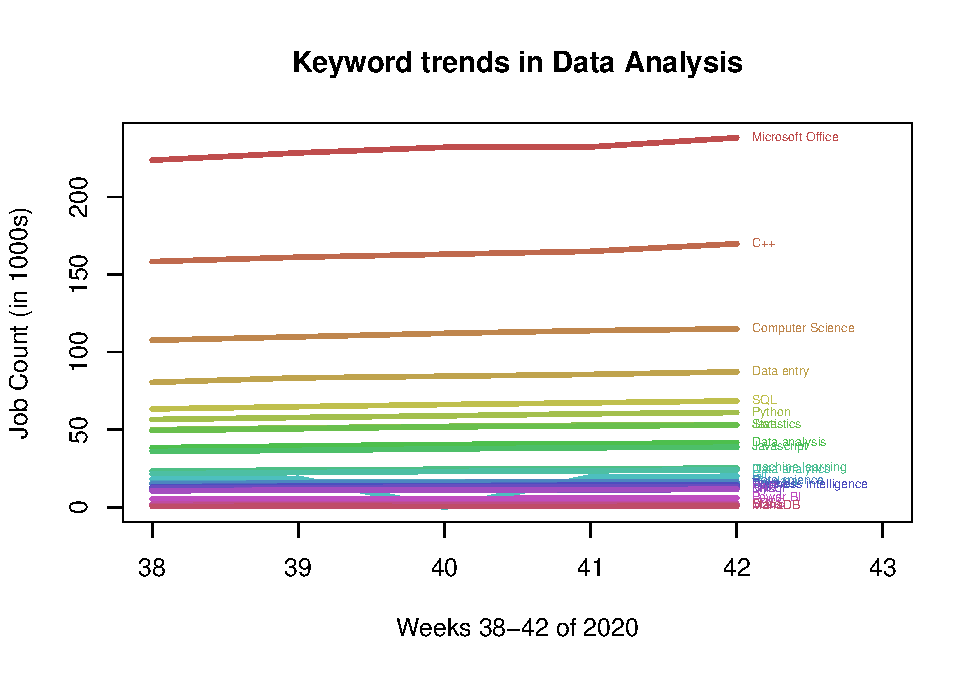
\includegraphics{graphics/chunk-plotting-jobs-trends-intro-1.pdf}

\begin{Shaded}
\begin{Highlighting}[]
\NormalTok{do.nothing =}\StringTok{ }\KeywordTok{plotJobs}\NormalTok{(jobs.subset, }\DataTypeTok{myy.lim =} \KeywordTok{c}\NormalTok{(}\DecValTok{0}\NormalTok{,}\DecValTok{42}\NormalTok{) );}
\end{Highlighting}
\end{Shaded}

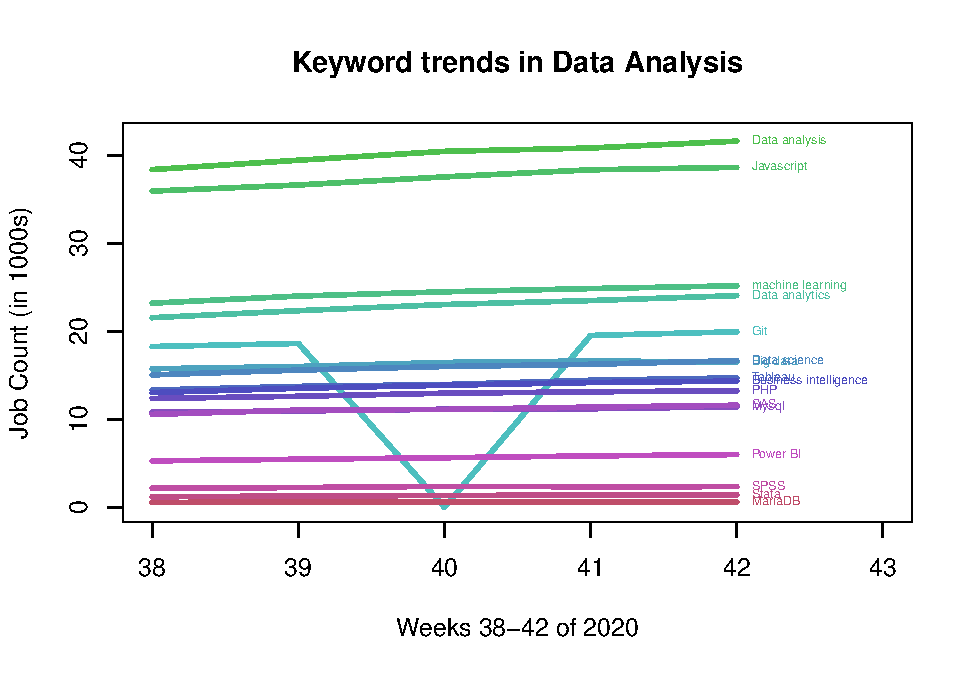
\includegraphics{graphics/chunk-plotting-jobs-trends-intro-2.pdf}

\hypertarget{initial-perspective}{%
\paragraph{Initial Perspective}\label{initial-perspective}}

{[}What is your initial ``perspective'' of this data, now that you see
it? Why are the lines ``parallel-ish''? What kind of a trend is that?

Now comment on the line of data for ``Data analysis''. How is it
trending? How does it compare to other Search-Query Words?

What is your first perspective?

{]}

\hypertarget{missing-data-git-week-40}{%
\paragraph{Missing Data ``Git'' Week
40?}\label{missing-data-git-week-40}}

\begin{Shaded}
\begin{Highlighting}[]
\NormalTok{do.nothing =}\StringTok{ }\KeywordTok{plotJobs}\NormalTok{(jobs.subset, }\DataTypeTok{myy.lim =} \KeywordTok{c}\NormalTok{(}\DecValTok{0}\NormalTok{,}\DecValTok{20}\NormalTok{) );}
\end{Highlighting}
\end{Shaded}

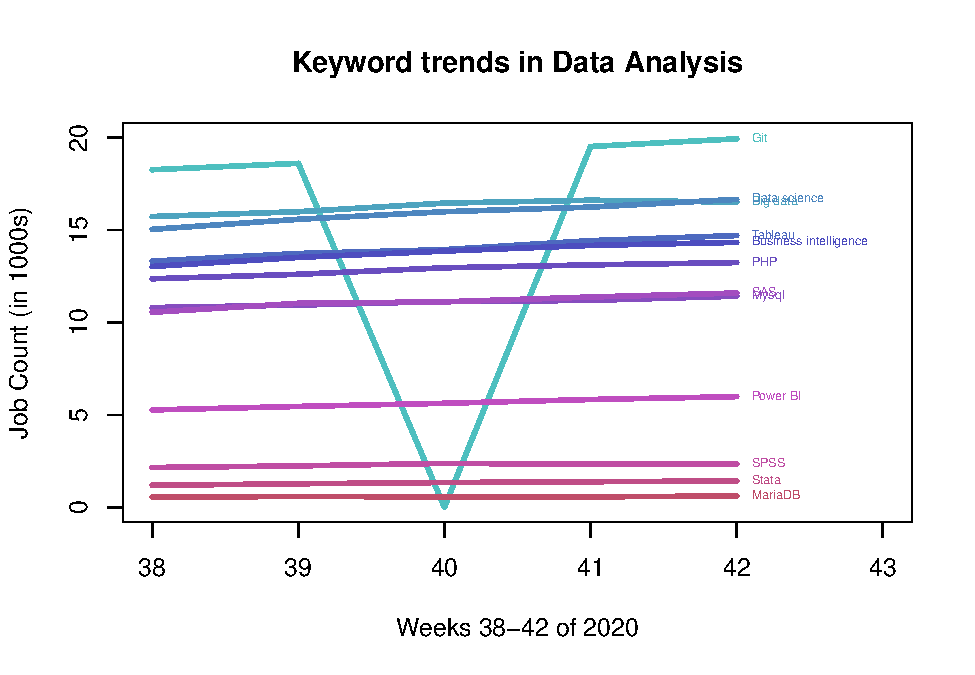
\includegraphics{graphics/chunk-plotting-jobs-trends-github-problem-1.pdf}

\textbf{Git-40/Git-41 data history, notice the date-time and file sizes
\ldots{}}

\textbf{Source: Data provenance history}

\textbf{Source: Data provenance history}

{[}Is this data missing or did it just drop to zero that week? How does
this relate to the other data (remember the idea of ``continuity'' in
mathematics)? What should you do about it?{]}

\begin{Shaded}
\begin{Highlighting}[]
\NormalTok{idxs.week}\FloatTok{.40}\NormalTok{ =}\StringTok{ }\KeywordTok{which}\NormalTok{(jobs.subset}\OperatorTok{$}\NormalTok{year.week }\OperatorTok{==}\StringTok{ }\FloatTok{2020.40}\NormalTok{);}
\NormalTok{idxs.Git     =}\StringTok{ }\KeywordTok{which}\NormalTok{(jobs.subset}\OperatorTok{$}\NormalTok{search.query }\OperatorTok{==}\StringTok{ "Git"}\NormalTok{);}

\CommentTok{\# set notation}
\NormalTok{my.idx =}\StringTok{ }\KeywordTok{intersect}\NormalTok{(idxs.Git,idxs.week}\FloatTok{.40}\NormalTok{);}

\NormalTok{jobs.subset[idxs.Git,];}
\end{Highlighting}
\end{Shaded}

\begin{verbatim}
##     year.week search.query job.count job.count.k
## 30    2020.38          Git     18270      18.270
## 211   2020.39          Git     18617      18.617
## 542   2020.40          Git         0       0.000
## 573   2020.41          Git     19528      19.528
## 753   2020.42          Git     19945      19.945
\end{verbatim}

\begin{Shaded}
\begin{Highlighting}[]
\NormalTok{jobs.subset[my.idx,];}
\end{Highlighting}
\end{Shaded}

\begin{verbatim}
##     year.week search.query job.count job.count.k
## 542    2020.4          Git         0           0
\end{verbatim}

\begin{Shaded}
\begin{Highlighting}[]
\CommentTok{\#\# change this if you feel appropriate?  To what number? }
\NormalTok{jobs.subset[my.idx,}\DecValTok{3}\NormalTok{] =}\StringTok{ }\DecValTok{0}\NormalTok{;         }\CommentTok{\# job.count}
\NormalTok{jobs.subset[my.idx,}\DecValTok{3}\NormalTok{] =}\StringTok{ }\DecValTok{0}\OperatorTok{/}\DecValTok{1000}\NormalTok{;    }\CommentTok{\# job.count.k (in thousands) ...}

\NormalTok{do.nothing =}\StringTok{ }\KeywordTok{plotJobs}\NormalTok{(jobs.subset, }\DataTypeTok{myy.lim =} \KeywordTok{c}\NormalTok{(}\DecValTok{0}\NormalTok{,}\DecValTok{20}\NormalTok{) );}
\end{Highlighting}
\end{Shaded}

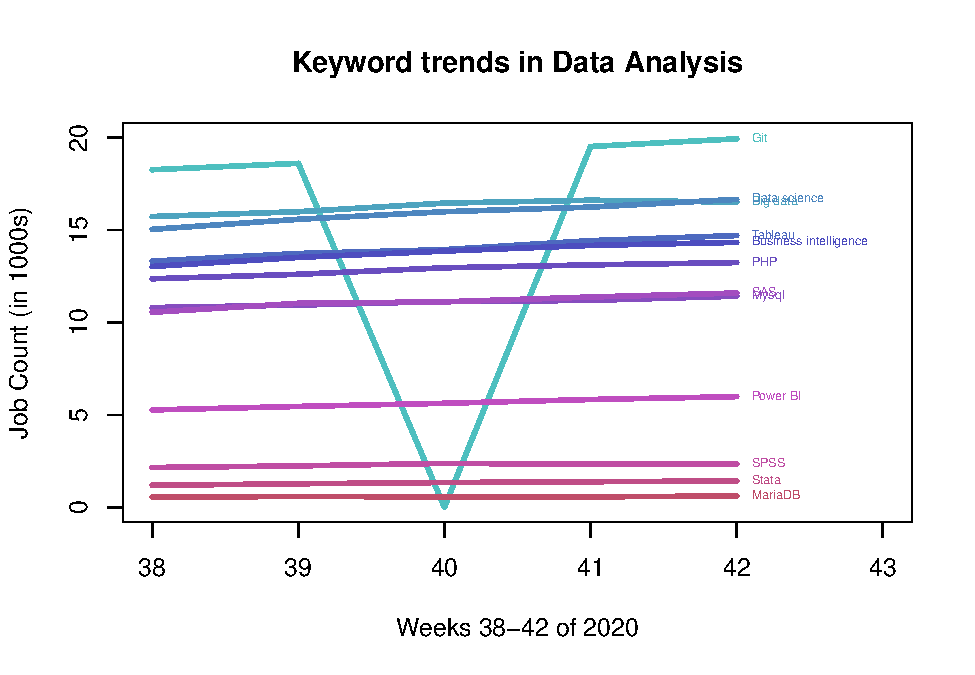
\includegraphics{graphics/chunk-plotting-jobs-trends-github-solution-1.pdf}

\hypertarget{is-microsoft-office-bigger-than-c}{%
\paragraph{Is ``Microsoft Office'' bigger than
``C++''?}\label{is-microsoft-office-bigger-than-c}}

I use the term ``bigger'' or ``better'' intentionally. We are comparing
two items, and these are generic ways of communicating such a
comparison. In context of this data problem, a formalized form of the
question would be something like: ``Utilizing job count for a given
search query, determine if the query `Microsoft Office' has a larger job
count than the query `C++'?'' This question will need to be formalized
if we are trying to draw specific conclusions, but the initiation of
analysis ``which is bigger'' allows us to understand what the data says
or does not say, through exploration.

To answer the question:

Mathematically, if two lines are parallel, and one is above the other,
can we use \textbf{distance} to draw a conclusion? Now, many times in
statistics we deal with noise in the data, it is not ``deterministic''
but ``stochastic'' \ldots{} so we need to understand the variability.
Based on the data we see, can we not use ``parallel-line'' logic to
conclude that they are different? This is one dimension of EDA, use
mathematics. (``mathematics'')

\begin{Shaded}
\begin{Highlighting}[]
\NormalTok{do.nothing =}\StringTok{ }\KeywordTok{plotJobs}\NormalTok{(jobs.subset, }\DataTypeTok{myy.lim =} \KeywordTok{c}\NormalTok{(}\DecValTok{80}\NormalTok{,}\DecValTok{250}\NormalTok{) );}
\end{Highlighting}
\end{Shaded}

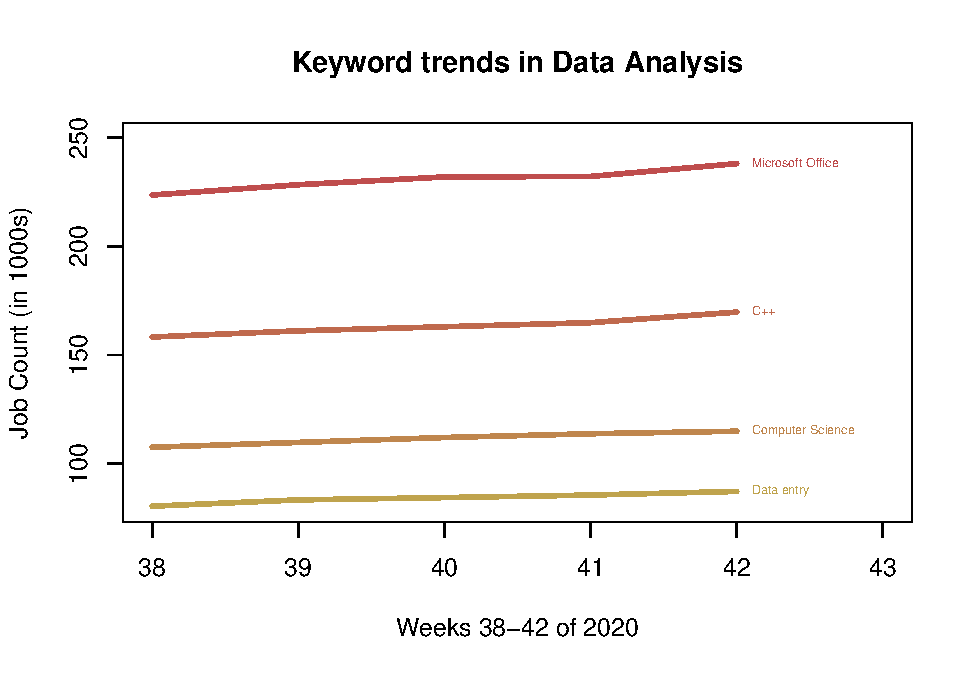
\includegraphics{graphics/chunk-plotting-jobs-trends-microsoft-1.pdf}

\begin{Shaded}
\begin{Highlighting}[]
\KeywordTok{boxplotJobQueryComparison}\NormalTok{(jobs.subset, }\StringTok{"Microsoft Office"}\NormalTok{, }\StringTok{"C++"}\NormalTok{);}
\end{Highlighting}
\end{Shaded}

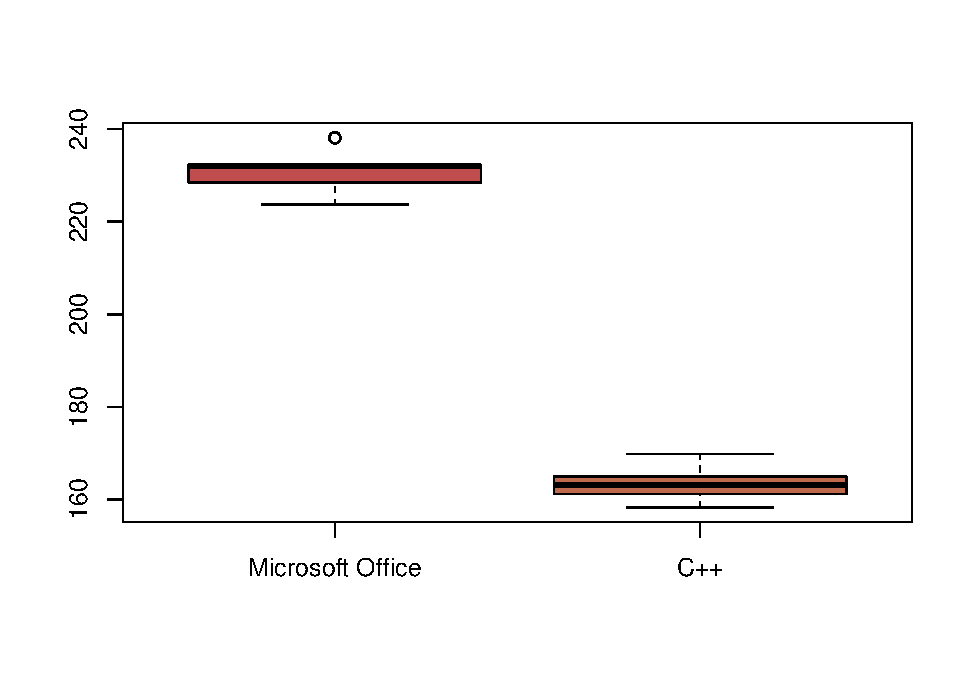
\includegraphics{graphics/chunk-plotting-jobs-trends-microsoft-2.pdf}
Tukey invented the boxplot as a nice EDA representation of the data.
What logical inference can we make about the distances between the
boxplots and the fact that no data is overlapping. This is another
dimension of EDA, use ``distance'' and the boxplot ``IQR'' to compare
two elements. What conclusion would we make? (``boxplot'')

{[}Can we conclude the data are different based on ``mathematics'' or
``boxplot''?

Would a formal ``inferential statistical test'' tell us something
different than logical inference?

How do you think ``formal tests'' were derived if not from
``mathematics'' and ``boxplot'' (EDA)?{]}

\begin{Shaded}
\begin{Highlighting}[]
\CommentTok{\# courage in trusting your intuition may require a fall{-}back ... for those that need it ...}

\KeywordTok{t.test.jobs}\NormalTok{(jobs.subset, }\StringTok{"Microsoft Office"}\NormalTok{, }\StringTok{"C++"}\NormalTok{); }
\end{Highlighting}
\end{Shaded}

\begin{verbatim}
## 
##  Welch Two Sample t-test
## 
## data:  x and y
## t = 22.016, df = 7.6613, p-value = 0.00000003332
## alternative hypothesis: true difference in means is not equal to 0
## 95 percent confidence interval:
##  60.31098 74.54582
## sample estimates:
## mean of x mean of y 
##  230.8730  163.4446
\end{verbatim}

\hypertarget{is-statistics-bigger-than-java}{%
\paragraph{Is ``Statistics'' bigger than
``Java''?}\label{is-statistics-bigger-than-java}}

\begin{Shaded}
\begin{Highlighting}[]
\NormalTok{do.nothing =}\StringTok{ }\KeywordTok{plotJobs}\NormalTok{(jobs.subset, }\DataTypeTok{myy.lim =} \KeywordTok{c}\NormalTok{(}\DecValTok{49}\NormalTok{,}\DecValTok{53}\NormalTok{) );}
\end{Highlighting}
\end{Shaded}

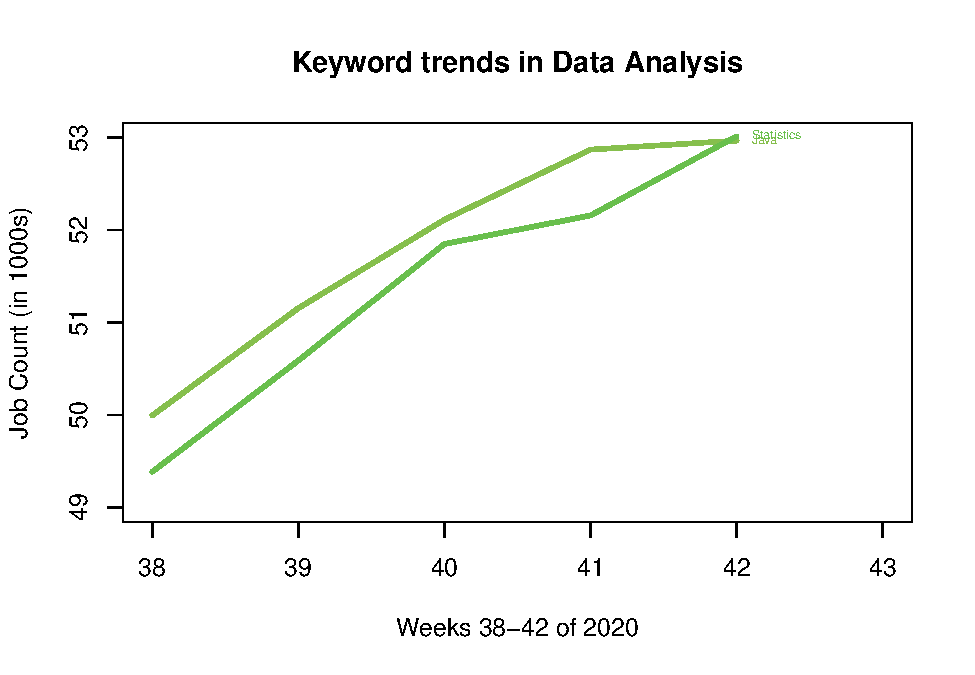
\includegraphics{graphics/chunk-plotting-jobs-trends-statistics-1.pdf}

\begin{Shaded}
\begin{Highlighting}[]
\NormalTok{do.nothing =}\StringTok{ }\KeywordTok{boxplotJobQueryComparison}\NormalTok{(jobs.subset, }\StringTok{"Statistics"}\NormalTok{, }\StringTok{"Java"}\NormalTok{);}
\end{Highlighting}
\end{Shaded}

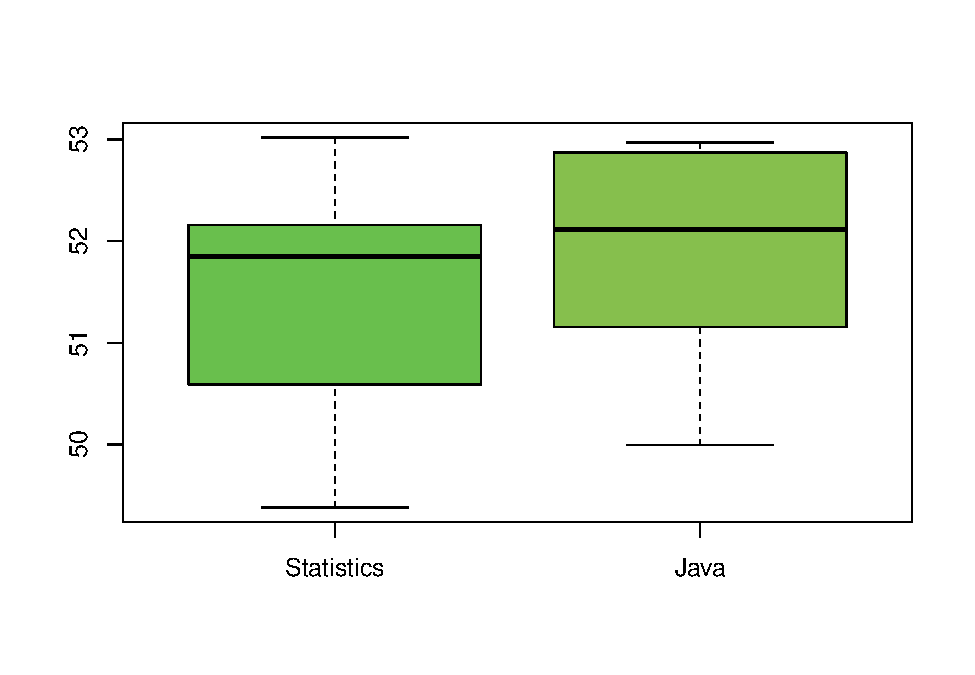
\includegraphics{graphics/chunk-plotting-jobs-trends-statistics-2.pdf}

For this data, I can descriptively report that the third-quartile
\texttt{Q3} of ``Statistics'' is about equal to the \texttt{median} of
``Java''. The inter-quartile range (\texttt{IQR}) of each overlap. The
minimum value of ``Java'' is larger than the minimum value of
``Statistics''. The maximum value of ``Java'' is slightly smaller than
the maximum value of ``Statistics''.

{[}Use ``mathematics'' and ``boxplot'' and ``ttest'' to answer the
question: Is ``Statistics'' bigger than ``Java''?{]}

\hypertarget{what-about-data-science-and-big-data}{%
\paragraph{What about ``Data science'' and ``Big
data''?}\label{what-about-data-science-and-big-data}}

\begin{Shaded}
\begin{Highlighting}[]
\NormalTok{do.nothing =}\StringTok{ }\KeywordTok{plotJobs}\NormalTok{(jobs.subset, }\DataTypeTok{myy.lim =} \KeywordTok{c}\NormalTok{(}\DecValTok{14}\NormalTok{,}\DecValTok{17}\NormalTok{) );}
\end{Highlighting}
\end{Shaded}

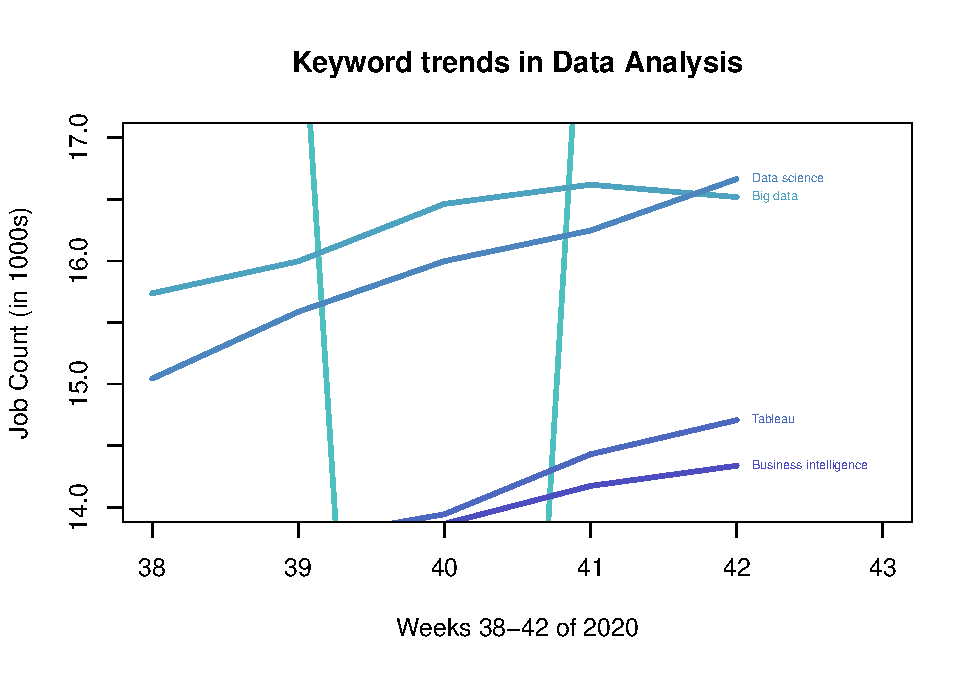
\includegraphics{graphics/chunk-plotting-jobs-trends-big-data-1.pdf}

\begin{Shaded}
\begin{Highlighting}[]
\KeywordTok{boxplotJobQueryComparison}\NormalTok{(jobs.subset, }\StringTok{"Data science"}\NormalTok{, }\StringTok{"Big data"}\NormalTok{);}
\end{Highlighting}
\end{Shaded}

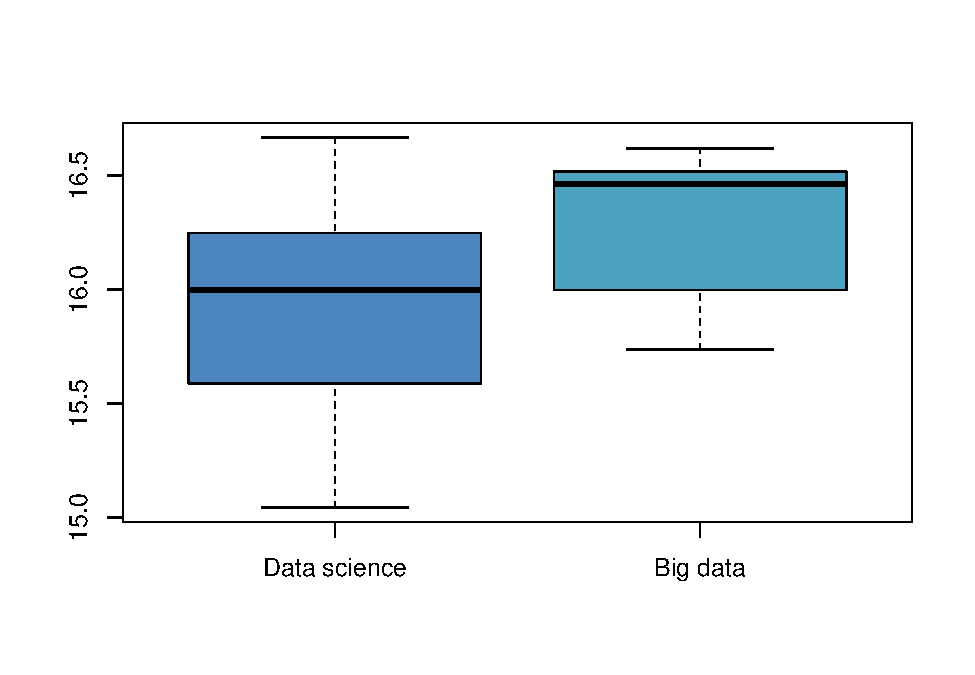
\includegraphics{graphics/chunk-plotting-jobs-trends-big-data-2.pdf}

{[}Use ``mathematics'' and ``boxplot'' and ``ttest'' to make a
conclusion.

Next, think carefully about the nature of the data. Is the
``collection-approach'' flawed to make a conclusion comparing job-counts
of these specific keywords? How likely is it that a single-job posting
may have both keywords?

This is an example where ``data-integrity'' knowledge would surpass the
other three logical conclusions.

This intuition requires an understanding of what mathematicians call
``set theory''. If I am doing an independent search on keywords, is it
possible that one job would show up in multiple searches. That is, being
counted twice or more.

Intuition and logic would also allow us to conclude that our other
comparisons are ``very likely okay''. Why?

What would be an improved approach to collecting the data that would
allow me to more accurately compare these two keywords?

This is representative of why exploratory data analysis is essential. It
provides us insight into the domain and highlights the need for better
data, if we can find it.

{]}

\hypertarget{conclusions-on-logical-inference}{%
\subsubsection{Conclusions on logical
inference}\label{conclusions-on-logical-inference}}

Distance is a fundamental unit of comparison. We can use our
``mathematical'' understanding of distance. We can use an ``EDA''
understanding of the data (e.g., the boxplot). We need to understand the
data sourcing and how that will relate to the logical conclusions we are
trying to draw.

When we transition to ``confirmatory inferential statistics'', we cannot
leave our understanding of ``maths'' and ``EDA'' behind. They are the
foundation from which ``inferential statistics'' is built. They are
``logical inference''.

\hypertarget{computing-distances}{%
\subsection{COMPUTING DISTANCES}\label{computing-distances}}

If you recall, we had a notebook on collecting data from Wikipedia. We
documented the ``data-provenance'' protocols to make this happen. We
have documented and can replicate our data-collection strategies.

\hypertarget{points-data-provenance-defined}{%
\subsubsection{(10 points) Data Provenance
defined}\label{points-data-provenance-defined}}

Imagine you are preparing for a job interview. Write a 90-second blurb
describing ``what is data provenance'' and ``why it matters''. I would
suggest the STAR(S) approach mentioned in one of the notebooks.
Reference the ``Wikipedia'' project as an example of how one can
implement the features.

{[}What is data provenance?

Probably about 200-250 words (with the 90 second limit) {]}

\hypertarget{geospatial-distances}{%
\subsubsection{Geospatial distances}\label{geospatial-distances}}

``Geo-spatial'' studies are becoming much more common in the ``data
analytics'' community, so let's use basic ``latitude/longitude'' data to
formally talk about ``distance.''

So we will look at the 50 state capitals of America (USA). Before that,
let's examine some basic principles of distances using my hometown.

\hypertarget{points-distance-from-one-input-to-multiple-outputs}{%
\subsubsection{(5 points) Distance from one input to multiple
outputs}\label{points-distance-from-one-input-to-multiple-outputs}}

\hypertarget{my-hometown-columbia-falls-montana-cfalls}{%
\paragraph{\texorpdfstring{My Hometown ``Columbia Falls, Montana''
\texttt{cfalls}}{My Hometown ``Columbia Falls, Montana'' cfalls}}\label{my-hometown-columbia-falls-montana-cfalls}}

\begin{itemize}
\tightlist
\item
  Find all ZIP codes within 22 miles of Columbia Falls, MT
  \texttt{cfalls} (use lat/long provide from the Wikipedia
  lookup)\ldots{} build the bounding ``box'' and perform the post-hoc
  ``radial distance'' computations (as we did in the homework).
\end{itemize}

\begin{Shaded}
\begin{Highlighting}[]
\CommentTok{\# copy/paste \_\_student\_access\_\_/\_SECRET\_/\_SECRET\_database\_.txt into console...  or this won\textquotesingle{}t work}

\NormalTok{cfalls.latitude =}\StringTok{ }\FloatTok{48.37028}\NormalTok{; }
\NormalTok{cfalls.longitude =}\StringTok{ }\FloatTok{{-}114.18889}\NormalTok{;}
\NormalTok{my.radius =}\StringTok{ }\DecValTok{22}\NormalTok{; my.units =}\StringTok{ "mi"}\NormalTok{; }\CommentTok{\#miles}

\CommentTok{\# THIS is where these exam functions live ...}
\CommentTok{\# source\_url( paste0(path.github,"misc/functions{-}midterm{-}F2000.R") );  \# should be 2020 ... oh well}




\NormalTok{cfalls.info =}\StringTok{ }\KeywordTok{getNeighborsFromLatLong}\NormalTok{(}\DecValTok{22}\NormalTok{, }\FloatTok{48.37028}\NormalTok{, }\FloatTok{{-}114.18889}\NormalTok{, }\StringTok{"mi"}\NormalTok{);}
\end{Highlighting}
\end{Shaded}

\begin{verbatim}
## [1] "The QUERY returned ...  13  ... NEIGHBORS"
\end{verbatim}

\begin{Shaded}
\begin{Highlighting}[]
\NormalTok{cfalls.info}\OperatorTok{$}\NormalTok{neighbors;}
\end{Highlighting}
\end{Shaded}

\begin{verbatim}
##    zipcode latitude longitude           city state_long state
## 1    59901 48.21124 -114.2939      KALISPELL    MONTANA    MT
## 2    59903 48.19303 -114.3579      KALISPELL    MONTANA    MT
## 3    59904 48.19452 -114.3123      KALISPELL    MONTANA    MT
## 4    59912 48.36531 -114.1927 COLUMBIA FALLS    MONTANA    MT
## 5    59913 48.43674 -114.0507          CORAM    MONTANA    MT
## 6    59916 48.61750 -113.9095          ESSEX    MONTANA    MT
## 7    59919 48.38969 -114.0630   HUNGRY HORSE    MONTANA    MT
## 8    59920 48.06516 -114.5023           KILA    MONTANA    MT
## 9    59921 48.62189 -113.8739 LAKE MC DONALD    MONTANA    MT
## 10   59926 48.39134 -114.0393    MARTIN CITY    MONTANA    MT
## 11   59932 48.07931 -114.2389         SOMERS    MONTANA    MT
## 12   59936 48.49720 -113.9892   WEST GLACIER    MONTANA    MT
## 13   59937 48.40834 -114.3522      WHITEFISH    MONTANA    MT
\end{verbatim}

\begin{Shaded}
\begin{Highlighting}[]
\CommentTok{\#\#\#\#\#\#\#\#\#\#\#\#\#\# plotting \#\#\#\#\#\#\#\#\#\#\#\#\#\#}
\NormalTok{brown =}\StringTok{ "\#ffe4c4"}\NormalTok{;}
\NormalTok{green =}\StringTok{ "\#014421"}\NormalTok{;}

\NormalTok{my.state =}\StringTok{ "montana"}\NormalTok{;}
\NormalTok{my.state.color =}\StringTok{ "\#ffe4c4"}\NormalTok{;}

\NormalTok{my.county =}\StringTok{ "flathead"}\NormalTok{;}
\NormalTok{my.county.color =}\StringTok{ "\#014421"}\NormalTok{; }

\NormalTok{my.nearby.states =}\StringTok{ }\KeywordTok{c}\NormalTok{(}\StringTok{"idaho"}\NormalTok{, }\StringTok{"washington"}\NormalTok{, }\StringTok{"oregon"}\NormalTok{);}


\KeywordTok{plotNeighbors}\NormalTok{(cfalls.info, }
                    \DataTypeTok{state          =}\NormalTok{ my.state, }
                    \DataTypeTok{state.color    =}\NormalTok{ my.state.color,}
                    \DataTypeTok{state.border   =} \FloatTok{0.05}\NormalTok{,}
                    \DataTypeTok{county         =}\NormalTok{ my.county, }
                    \DataTypeTok{county.border   =} \FloatTok{0.05}\NormalTok{,  }\CommentTok{\# if you don\textquotesingle{}t see the box, increase this to like 0.75}
                    \DataTypeTok{county.color   =}\NormalTok{ my.county.color, }
                    \DataTypeTok{nearby.states  =}\NormalTok{ my.nearby.states); }
\end{Highlighting}
\end{Shaded}

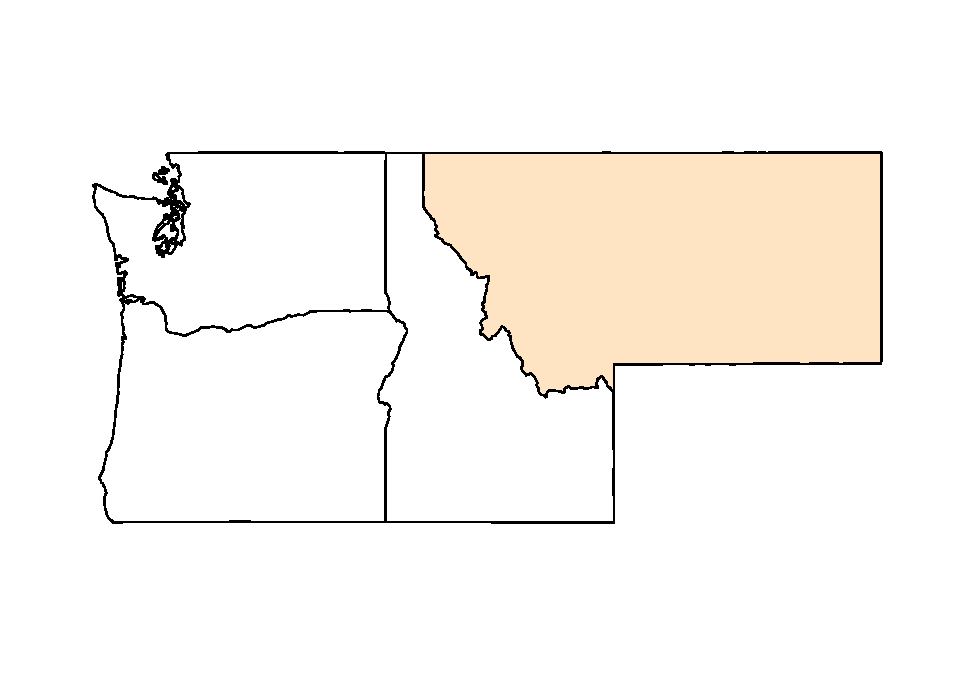
\includegraphics{graphics/chunk-distances-compute-cfalls-1.pdf}
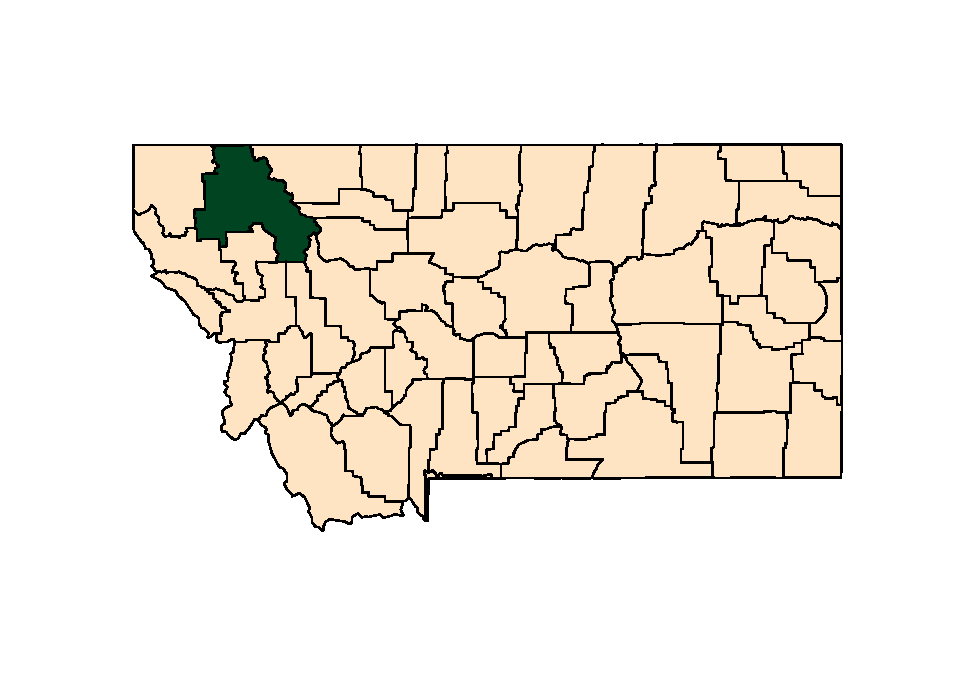
\includegraphics{graphics/chunk-distances-compute-cfalls-2.pdf}
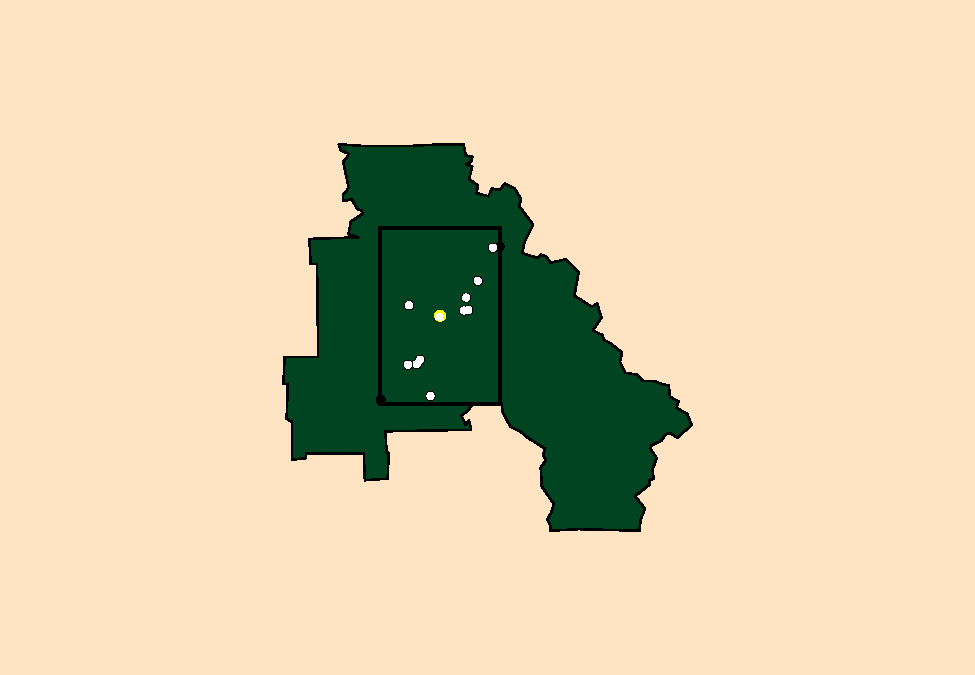
\includegraphics{graphics/chunk-distances-compute-cfalls-3.pdf}

{[} - why is the box not a square, but a rectangle? \ldots{} see
\texttt{factor.lat} and \texttt{factor.long} in function
\texttt{buildBoundingBoxFromRadiusAndGivenLatitudeLongitude} - critique
the visualization \ldots{} what do you like? what would make it
better?{]}

\hypertarget{your-hometown-of-something-like-it}{%
\paragraph{Your Hometown of something like
it}\label{your-hometown-of-something-like-it}}

Instead of \texttt{cfalls.info}, you do \texttt{hometown.info}

\begin{itemize}
\tightlist
\item
  a location in the continental US of your choosing (not in Montana,
  Alaska, or Hawaii). {[}Graphing will not work for Alaska/Hawaii,
  Alaska has ``boroughs'' not counties.{]}
\item
  find the latitude/longitude of the location you have selected (how and
  where to look that up?)
\item
  Initially start with a radius of \texttt{13\ miles}
\item
  When you run the code, note how many total ``neighbors''; if it is
  less than 20; increase the ``miles'' so at least 20 results are
  returned.
\item
  In the end, you should select a location and radius that works for
  you. And its visualization also works.
\item
  Be certain to review and update the parameters before calling these
  functions.
\end{itemize}

hometown.latitude = 00.00000; hometown.longitude = -000.00000; my.radius
= 13; my.units = ``mi''; \#miles hometown.info =
getNeighborsFromLatLong( ???? ); plotNeighbors(hometown.info, ????); \#
you are going to have to change some of these parameters \ldots{}

\begin{Shaded}
\begin{Highlighting}[]
\NormalTok{hometown.latitude =}\StringTok{ }\FloatTok{00.000}\NormalTok{; }
\NormalTok{hometown.longitude =}\StringTok{ }\FloatTok{{-}000.000}\NormalTok{;}
\NormalTok{my.radius =}\StringTok{ }\DecValTok{13}\NormalTok{; my.units =}\StringTok{ "mi"}\NormalTok{; }\CommentTok{\#miles}


\CommentTok{\# hometown.info = getNeighborsFromLatLong( ???? );}
\CommentTok{\# hometown.info$neighbors;}
\CommentTok{\# plotNeighbors(hometown.info, ????);  \# you are going to have to change some of these parameters ... }
\end{Highlighting}
\end{Shaded}

\hypertarget{u.s.-state-capitals-cities}{%
\subsubsection{U.S. State Capitals
(cities)}\label{u.s.-state-capitals-cities}}

From Wikipedia, we grabbed one page that listed the 50 U.S. cities that
are designated the capitals of each individual state in America (United
States of America).

Using the power of a \texttt{for-loop} we make our functions work for
us. We now have the data ready to go.

\begin{Shaded}
\begin{Highlighting}[]
\NormalTok{capitals =}\StringTok{ }\NormalTok{utils}\OperatorTok{::}\KeywordTok{read.csv}\NormalTok{( }\KeywordTok{paste0}\NormalTok{(path.mshaffer, }\StringTok{"\_data\_/state{-}capitals/final/state{-}capitals.txt"}\NormalTok{), }\DataTypeTok{header=}\OtherTok{TRUE}\NormalTok{, }\DataTypeTok{quote=}\StringTok{""}\NormalTok{, }\DataTypeTok{sep=}\StringTok{"|"}\NormalTok{);}

\KeywordTok{colnames}\NormalTok{(capitals) =}\StringTok{ }\KeywordTok{c}\NormalTok{(}\StringTok{"state"}\NormalTok{, }\StringTok{"capital"}\NormalTok{, }\StringTok{"latitude"}\NormalTok{, }\StringTok{"longitude"}\NormalTok{, }\StringTok{"capital.since"}\NormalTok{, }\StringTok{"area.sq.miles"}\NormalTok{, }\StringTok{"population.2019.est"}\NormalTok{, }\StringTok{"population.2019.est.MSA"}\NormalTok{, }\StringTok{"population.2019.est.CSA"}\NormalTok{, }\StringTok{"city.rank.in.state"}\NormalTok{, }\StringTok{"url"}\NormalTok{);}

\CommentTok{\# hack{-}add from https://en.wikipedia.org/wiki/ISO\_3166{-}2:US}
\CommentTok{\# }\AlertTok{TODO}\CommentTok{, grab this table "appropriately" as a new function}
\CommentTok{\# Is there a dictionary for shortened city names?}
\CommentTok{\# the long{-}field names is also an issue that needs to be improved upon in the next iteration.}

\NormalTok{capitals}\OperatorTok{$}\NormalTok{st =}\StringTok{ }\KeywordTok{c}\NormalTok{(}\StringTok{"AL"}\NormalTok{,}\StringTok{"AK"}\NormalTok{,}\StringTok{"AZ"}\NormalTok{,}\StringTok{"AR"}\NormalTok{,}\StringTok{"CA"}\NormalTok{,}\StringTok{"CO"}\NormalTok{,}\StringTok{"CT"}\NormalTok{,}\StringTok{"DE"}\NormalTok{,}\StringTok{"FL"}\NormalTok{,}\StringTok{"GA"}\NormalTok{,}\StringTok{"HI"}\NormalTok{,}\StringTok{"ID"}\NormalTok{,}\StringTok{"IL"}\NormalTok{,}\StringTok{"IN"}\NormalTok{,}\StringTok{"IA"}\NormalTok{,}\StringTok{"KS"}\NormalTok{,}\StringTok{"KY"}\NormalTok{,}\StringTok{"LA"}\NormalTok{,}\StringTok{"ME"}\NormalTok{,}\StringTok{"MD"}\NormalTok{,}\StringTok{"MA"}\NormalTok{,}\StringTok{"MI"}\NormalTok{,}\StringTok{"MN"}\NormalTok{,}\StringTok{"MS"}\NormalTok{,}\StringTok{"MO"}\NormalTok{,}\StringTok{"MT"}\NormalTok{,}\StringTok{"NE"}\NormalTok{,}\StringTok{"NV"}\NormalTok{,}\StringTok{"NH"}\NormalTok{,}\StringTok{"NJ"}\NormalTok{,}\StringTok{"NM"}\NormalTok{,}\StringTok{"NY"}\NormalTok{,}\StringTok{"NC"}\NormalTok{,}\StringTok{"ND"}\NormalTok{,}\StringTok{"OH"}\NormalTok{,}\StringTok{"OK"}\NormalTok{,}\StringTok{"OR"}\NormalTok{,}\StringTok{"PA"}\NormalTok{,}\StringTok{"RI"}\NormalTok{,}\StringTok{"SC"}\NormalTok{,}\StringTok{"SD"}\NormalTok{,}\StringTok{"TN"}\NormalTok{,}\StringTok{"TX"}\NormalTok{,}\StringTok{"UT"}\NormalTok{,}\StringTok{"VT"}\NormalTok{,}\StringTok{"VA"}\NormalTok{,}\StringTok{"WA"}\NormalTok{,}\StringTok{"WV"}\NormalTok{,}\StringTok{"WI"}\NormalTok{,}\StringTok{"WY"}\NormalTok{); }\CommentTok{\# ,"DC","AS","GU","MP","PR","UM","VI");}

\NormalTok{myLabels =}\StringTok{ }\KeywordTok{paste0}\NormalTok{(capitals}\OperatorTok{$}\NormalTok{capital, }\StringTok{", "}\NormalTok{, capitals}\OperatorTok{$}\NormalTok{st);}

\NormalTok{capitals;}
\end{Highlighting}
\end{Shaded}

\begin{verbatim}
##             state        capital latitude  longitude capital.since
## 1         Alabama     Montgomery 32.36167  -86.27917          1846
## 2          Alaska         Juneau 58.30000 -134.41600          1906
## 3         Arizona        Phoenix 33.45000 -112.06700          1912
## 4        Arkansas    Little Rock 34.73611  -92.33111          1821
## 5      California     Sacramento 38.58167 -121.49444          1854
## 6        Colorado         Denver 39.73917 -104.99028          1867
## 7     Connecticut       Hartford 41.76250  -72.67417          1875
## 8        Delaware          Dover 39.15806  -75.52444          1777
## 9         Florida    Tallahassee 30.45500  -84.25333          1824
## 10        Georgia        Atlanta 33.75500  -84.39000          1868
## 11         Hawaii       Honolulu 21.30694 -157.85833          1845
## 12          Idaho          Boise 43.61583 -116.20167          1865
## 13       Illinois    Springfield 39.79944  -89.65500          1837
## 14        Indiana   Indianapolis 39.76861  -86.15806          1825
## 15           Iowa     Des Moines 41.59083  -93.62083          1857
## 16         Kansas         Topeka 39.05583  -95.68944          1856
## 17       Kentucky      Frankfort 38.20000  -84.86700          1792
## 18      Louisiana    Baton Rouge 30.44750  -91.17861          1880
## 19          Maine        Augusta 44.31056  -69.77944          1832
## 20       Maryland      Annapolis 38.97306  -76.50111          1694
## 21  Massachusetts         Boston 42.35806  -71.06361          1630
## 22       Michigan        Lansing 42.73361  -84.54667          1847
## 23      Minnesota     Saint Paul 44.94417  -93.09361          1849
## 24    Mississippi        Jackson 32.29889  -90.18472          1821
## 25       Missouri Jefferson City 38.57667  -92.17361          1826
## 26        Montana         Helena 46.59111 -112.02028          1875
## 27       Nebraska        Lincoln 40.80889  -96.67889          1867
## 28         Nevada    Carson City 39.16444 -119.76694          1861
## 29  New Hampshire        Concord 43.20667  -71.53806          1808
## 30     New Jersey        Trenton 40.22384  -74.76362          1784
## 31     New Mexico       Santa Fe 35.66722 -105.96444          1610
## 32       New York         Albany 42.65250  -73.75722          1797
## 33 North Carolina        Raleigh 35.76700  -78.63300          1792
## 34   North Dakota       Bismarck 46.80833 -100.78361          1883
## 35           Ohio       Columbus 39.96222  -83.00056          1816
## 36       Oklahoma  Oklahoma City 35.46861  -97.52139          1910
## 37         Oregon          Salem 44.93917 -123.03944          1855
## 38   Pennsylvania     Harrisburg 40.26972  -76.87556          1812
## 39   Rhode Island     Providence 41.82361  -71.42222          1900
## 40 South Carolina       Columbia 34.00056  -81.03472          1786
## 41   South Dakota         Pierre 44.37250 -100.32000          1889
## 42      Tennessee      Nashville 36.16667  -86.78333          1826
## 43          Texas         Austin 30.26722  -97.74306          1839
## 44           Utah Salt Lake City 40.76083 -111.89111          1858
## 45        Vermont     Montpelier 44.25944  -72.57583          1805
## 46       Virginia       Richmond 37.53300  -77.46700          1780
## 47     Washington        Olympia 47.03778 -122.90083          1853
## 48  West Virginia     Charleston 38.34722  -81.63333          1885
## 49      Wisconsin        Madison 43.07472  -89.38417          1838
## 50        Wyoming       Cheyenne 41.14000 -104.82028          1869
##    area.sq.miles population.2019.est population.2019.est.MSA
## 1         159.80              198525                  373290
## 2        2716.70               32113                   32113
## 3         517.60             1680992                 4948203
## 4         116.20              197312                  742384
## 5          97.90              513624                 2363730
## 6         153.30              727211                 2967239
## 7          17.30              122105                 1204877
## 8          22.40               38079                  180786
## 9          95.70              194500                  387227
## 10        133.50              506811                 6020364
## 11         68.40              345064                  974563
## 12         63.80              228959                  749202
## 13         54.00              114230                  206868
## 14        361.50              876384                 2074537
## 15         75.80              214237                  699292
## 16         56.00              125310                  231969
## 17         14.70               27679                   73663
## 18         76.80              220236                  854884
## 19         55.40               18681                  122302
## 20          6.73               39174                 2800053
## 21         89.60              692600                 4873019
## 22         35.00              118210                  550391
## 23         52.80              308096                 3654908
## 24        104.90              160628                  594806
## 25         27.30               42838                  151235
## 26         14.00               32315                   77414
## 27         74.60              289102                  336374
## 28        143.40               55916                   55916
## 29         64.30               43627                  151391
## 30          7.66               83203                  367430
## 31         37.30               84683                  150358
## 32         21.40               96460                  880381
## 33        114.60              474069                 1390785
## 34         26.90               73529                  128949
## 35        210.30              898553                 2122271
## 36        620.30              655057                 1408950
## 37         45.70              174365                  433903
## 38          8.11               49528                  577941
## 39         18.50              179883                 1624578
## 40        125.20              131674                  838433
## 41         13.00               13646                   20672
## 42        525.90              670820                 1934317
## 43        305.10              978908                 2227083
## 44        109.10              200567                 1232696
## 45         10.20                7855                      NA
## 46         60.10              230436                 1291900
## 47         16.70               46478                  290536
## 48         31.60               46536                  257074
## 49         68.70              259680                  664865
## 50         21.10               64235                   99500
##    population.2019.est.CSA city.rank.in.state
## 1                   461516                  2
## 2                       NA                  3
## 3                  5002221                  1
## 4                   908941                  1
## 5                  2639124                  6
## 6                  3617927                  1
## 7                  1470083                  3
## 8                  7209620                  2
## 9                       NA                  7
## 10                 6853392                  1
## 11                      NA                  1
## 12                  831235                  1
## 13                  306399                  6
## 14                 2457286                  1
## 15                  877991                  1
## 16                      NA                  4
## 17                  745033                 15
## 18                      NA                  2
## 19                      NA                  8
## 20                 9814928                  7
## 21                 8287710                  1
## 22                      NA                  5
## 23                 4027861                  2
## 24                  674340                  1
## 25                      NA                 15
## 26                      NA                  6
## 27                  357887                  2
## 28                  637973                  6
## 29                 8287710                  3
## 30                22589036                 10
## 31                 1158464                  4
## 32                 1167594                  6
## 33                 2079687                  2
## 34                      NA                  2
## 35                 2525639                  1
## 36                 1481542                  1
## 37                 3259710                  3
## 38                 1271801                  9
## 39                 8287710                  1
## 40                  963048                  2
## 41                      NA                  8
## 42                 2062547                  1
## 43                      NA                  4
## 44                 2641048                  1
## 45                      NA                  6
## 46                      NA                  4
## 47                 4903675                 24
## 48                  776694                  1
## 49                  892661                  2
## 50                      NA                  1
##                                                        url st
## 1        https://en.wikipedia.org/wiki/Montgomery,_Alabama AL
## 2             https://en.wikipedia.org/wiki/Juneau,_Alaska AK
## 3           https://en.wikipedia.org/wiki/Phoenix,_Arizona AZ
## 4      https://en.wikipedia.org/wiki/Little_Rock,_Arkansas AR
## 5     https://en.wikipedia.org/wiki/Sacramento,_California CA
## 6                     https://en.wikipedia.org/wiki/Denver CO
## 7      https://en.wikipedia.org/wiki/Hartford,_Connecticut CT
## 8            https://en.wikipedia.org/wiki/Dover,_Delaware DE
## 9       https://en.wikipedia.org/wiki/Tallahassee,_Florida FL
## 10                   https://en.wikipedia.org/wiki/Atlanta GA
## 11                  https://en.wikipedia.org/wiki/Honolulu HI
## 12              https://en.wikipedia.org/wiki/Boise,_Idaho ID
## 13     https://en.wikipedia.org/wiki/Springfield,_Illinois IL
## 14              https://en.wikipedia.org/wiki/Indianapolis IN
## 15          https://en.wikipedia.org/wiki/Des_Moines,_Iowa IA
## 16            https://en.wikipedia.org/wiki/Topeka,_Kansas KS
## 17       https://en.wikipedia.org/wiki/Frankfort,_Kentucky KY
## 18    https://en.wikipedia.org/wiki/Baton_Rouge,_Louisiana LA
## 19            https://en.wikipedia.org/wiki/Augusta,_Maine ME
## 20       https://en.wikipedia.org/wiki/Annapolis,_Maryland MD
## 21                    https://en.wikipedia.org/wiki/Boston MA
## 22         https://en.wikipedia.org/wiki/Lansing,_Michigan MI
## 23     https://en.wikipedia.org/wiki/Saint_Paul,_Minnesota MN
## 24      https://en.wikipedia.org/wiki/Jackson,_Mississippi MS
## 25  https://en.wikipedia.org/wiki/Jefferson_City,_Missouri MO
## 26           https://en.wikipedia.org/wiki/Helena,_Montana MT
## 27         https://en.wikipedia.org/wiki/Lincoln,_Nebraska NE
## 28       https://en.wikipedia.org/wiki/Carson_City,_Nevada NV
## 29    https://en.wikipedia.org/wiki/Concord,_New_Hampshire NH
## 30       https://en.wikipedia.org/wiki/Trenton,_New_Jersey NJ
## 31      https://en.wikipedia.org/wiki/Santa_Fe,_New_Mexico NM
## 32          https://en.wikipedia.org/wiki/Albany,_New_York NY
## 33   https://en.wikipedia.org/wiki/Raleigh,_North_Carolina NC
## 34    https://en.wikipedia.org/wiki/Bismarck,_North_Dakota ND
## 35            https://en.wikipedia.org/wiki/Columbus,_Ohio OH
## 36             https://en.wikipedia.org/wiki/Oklahoma_City OK
## 37             https://en.wikipedia.org/wiki/Salem,_Oregon OR
## 38  https://en.wikipedia.org/wiki/Harrisburg,_Pennsylvania PA
## 39  https://en.wikipedia.org/wiki/Providence,_Rhode_Island RI
## 40  https://en.wikipedia.org/wiki/Columbia,_South_Carolina SC
## 41      https://en.wikipedia.org/wiki/Pierre,_South_Dakota SD
## 42      https://en.wikipedia.org/wiki/Nashville,_Tennessee TN
## 43             https://en.wikipedia.org/wiki/Austin,_Texas TX
## 44            https://en.wikipedia.org/wiki/Salt_Lake_City UT
## 45       https://en.wikipedia.org/wiki/Montpelier,_Vermont VT
## 46        https://en.wikipedia.org/wiki/Richmond,_Virginia VA
## 47       https://en.wikipedia.org/wiki/Olympia,_Washington WA
## 48 https://en.wikipedia.org/wiki/Charleston,_West_Virginia WV
## 49        https://en.wikipedia.org/wiki/Madison,_Wisconsin WI
## 50         https://en.wikipedia.org/wiki/Cheyenne,_Wyoming WY
\end{verbatim}

\hypertarget{initial-plotting}{%
\paragraph{Initial Plotting}\label{initial-plotting}}

\begin{itemize}
\tightlist
\item
  Plot the data on \texttt{usmap} (ggplot2)
\end{itemize}

\begin{Shaded}
\begin{Highlighting}[]
\NormalTok{latlong =}\StringTok{ }\KeywordTok{removeAllColumnsBut}\NormalTok{(capitals,}\KeywordTok{c}\NormalTok{( }\StringTok{"state"}\NormalTok{, }\StringTok{"st"}\NormalTok{, }\StringTok{"capital"}\NormalTok{, }\StringTok{"latitude"}\NormalTok{, }\StringTok{"longitude"}\NormalTok{, }\StringTok{"population.2019.est"}\NormalTok{) );}

\CommentTok{\# first two elements have to be this}
\NormalTok{latlong =}\StringTok{ }\KeywordTok{moveColumnsInDataFrame}\NormalTok{(latlong, }\KeywordTok{c}\NormalTok{(}\StringTok{"longitude"}\NormalTok{,}\StringTok{"latitude"}\NormalTok{), }\StringTok{"before"}\NormalTok{, }\StringTok{"state"}\NormalTok{);}

\CommentTok{\# for transform to work}
\KeywordTok{library}\NormalTok{(usmap);    }
\NormalTok{latlong.transform =}\StringTok{ }\KeywordTok{usmap\_transform}\NormalTok{(latlong);}
\KeywordTok{library}\NormalTok{(ggplot2);}

\CommentTok{\#\#\# plot\_usmap ...  }

\KeywordTok{plot\_usmap}\NormalTok{(}\DataTypeTok{fill =} \StringTok{"\#53565A"}\NormalTok{, }\DataTypeTok{alpha =} \FloatTok{0.25}\NormalTok{) }\OperatorTok{+}
\StringTok{  }\NormalTok{ggrepel}\OperatorTok{::}\KeywordTok{geom\_label\_repel}\NormalTok{(}\DataTypeTok{data =}\NormalTok{ latlong.transform,}
             \KeywordTok{aes}\NormalTok{(}\DataTypeTok{x =}\NormalTok{ longitude}\FloatTok{.1}\NormalTok{, }\DataTypeTok{y =}\NormalTok{ latitude}\FloatTok{.1}\NormalTok{, }\DataTypeTok{label =}\NormalTok{ capital),}
             \DataTypeTok{size =} \DecValTok{3}\NormalTok{, }\DataTypeTok{alpha =} \FloatTok{0.8}\NormalTok{,}
             \DataTypeTok{label.r =} \KeywordTok{unit}\NormalTok{(}\FloatTok{0.5}\NormalTok{, }\StringTok{"lines"}\NormalTok{), }\DataTypeTok{label.size =} \FloatTok{0.5}\NormalTok{,}
             \DataTypeTok{segment.color =} \StringTok{"\#981E32"}\NormalTok{, }\DataTypeTok{segment.size =} \DecValTok{1}\NormalTok{,}
             \DataTypeTok{seed =} \DecValTok{1002}\NormalTok{) }\OperatorTok{+}
\StringTok{  }\KeywordTok{scale\_size\_continuous}\NormalTok{(}\DataTypeTok{range =} \KeywordTok{c}\NormalTok{(}\DecValTok{1}\NormalTok{, }\DecValTok{16}\NormalTok{),}
                        \DataTypeTok{label =}\NormalTok{ scales}\OperatorTok{::}\NormalTok{comma) }\OperatorTok{+}
\StringTok{  }\KeywordTok{labs}\NormalTok{(}\DataTypeTok{title =} \StringTok{"U.S. State Capitals"}\NormalTok{,}
       \DataTypeTok{subtitle =} \StringTok{"Source: Wikipedia (October 2020)"}\NormalTok{) }\OperatorTok{+}
\StringTok{  }\KeywordTok{theme}\NormalTok{(}\DataTypeTok{legend.position =} \StringTok{"right"}\NormalTok{)}
\end{Highlighting}
\end{Shaded}

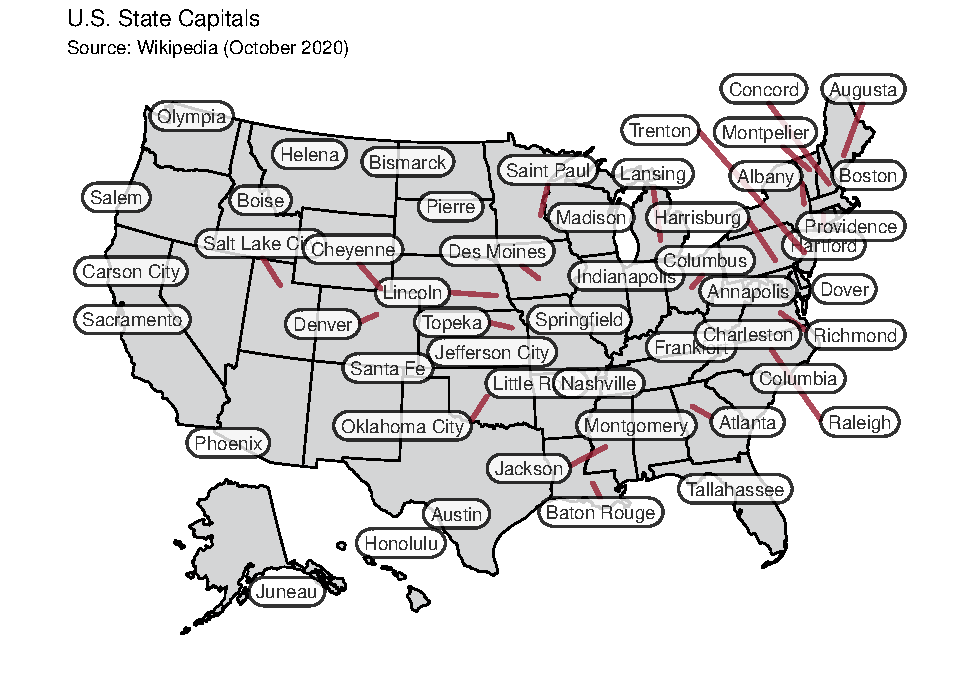
\includegraphics{graphics/chunk-distances-plot_usmap-1.pdf}

\begin{itemize}
\tightlist
\item
  Plot the data using maths \texttt{voronoi} (tripack)
\end{itemize}

\begin{Shaded}
\begin{Highlighting}[]
\NormalTok{colors =}\StringTok{ }\KeywordTok{rainbow}\NormalTok{(}\DecValTok{50}\NormalTok{, }\DataTypeTok{s =} \FloatTok{0.6}\NormalTok{, }\DataTypeTok{v =} \FloatTok{0.75}\NormalTok{);}

\CommentTok{\#\# initial visualization ...}
\KeywordTok{library}\NormalTok{(tripack);}
\CommentTok{\# plot( voronoi.mosaic(latlong[,4:3], duplicate="remove"), col=colors, xlab="");}
\KeywordTok{plot}\NormalTok{( }\KeywordTok{voronoi.mosaic}\NormalTok{(}\DataTypeTok{x =}\NormalTok{ latlong}\OperatorTok{$}\NormalTok{longitude, }\DataTypeTok{y =}\NormalTok{ latlong}\OperatorTok{$}\NormalTok{latitude), }\DataTypeTok{col=}\NormalTok{colors, }\DataTypeTok{xlab=}\StringTok{""}\NormalTok{);}
\KeywordTok{text}\NormalTok{(}\DataTypeTok{x =}\NormalTok{ latlong}\OperatorTok{$}\NormalTok{longitude, }\DataTypeTok{y =}\NormalTok{ latlong}\OperatorTok{$}\NormalTok{latitude, }\DataTypeTok{labels =}\NormalTok{ latlong}\OperatorTok{$}\NormalTok{capital, }\DataTypeTok{col=}\NormalTok{colors, }\DataTypeTok{cex=}\FloatTok{0.5}\NormalTok{);}
\end{Highlighting}
\end{Shaded}

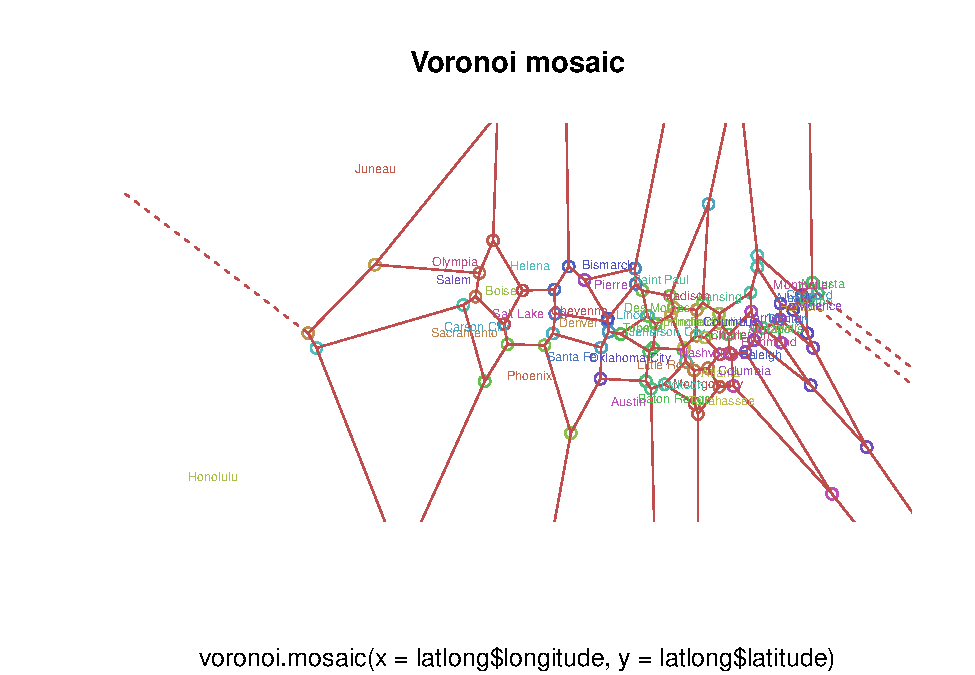
\includegraphics{graphics/chunk-distances-map-1.pdf}

\begin{itemize}
\tightlist
\item
  Plot the data on \texttt{map} (base)
\end{itemize}

\begin{Shaded}
\begin{Highlighting}[]
\CommentTok{\#\#\# how is any of the other visualizations really any better than a simple map ... with actual locations for Alaska/Hawaii?}
\KeywordTok{library}\NormalTok{(maps); }
\KeywordTok{map}\NormalTok{(}\StringTok{\textquotesingle{}state\textquotesingle{}}\NormalTok{, }\DataTypeTok{plot =} \OtherTok{TRUE}\NormalTok{, }\DataTypeTok{fill =} \OtherTok{FALSE}\NormalTok{, }
    \DataTypeTok{col =} \StringTok{"blue"}\NormalTok{, }\DataTypeTok{myborder =} \FloatTok{0.5}
\NormalTok{    );}
\KeywordTok{points}\NormalTok{(}\DataTypeTok{x =}\NormalTok{ latlong}\OperatorTok{$}\NormalTok{longitude, }\DataTypeTok{y =}\NormalTok{ latlong}\OperatorTok{$}\NormalTok{latitude, }
                  \DataTypeTok{col =} \StringTok{"red"}\NormalTok{, }\DataTypeTok{pch =} \StringTok{"*"}\NormalTok{, }\DataTypeTok{cex =} \DecValTok{1}\NormalTok{);}
\end{Highlighting}
\end{Shaded}

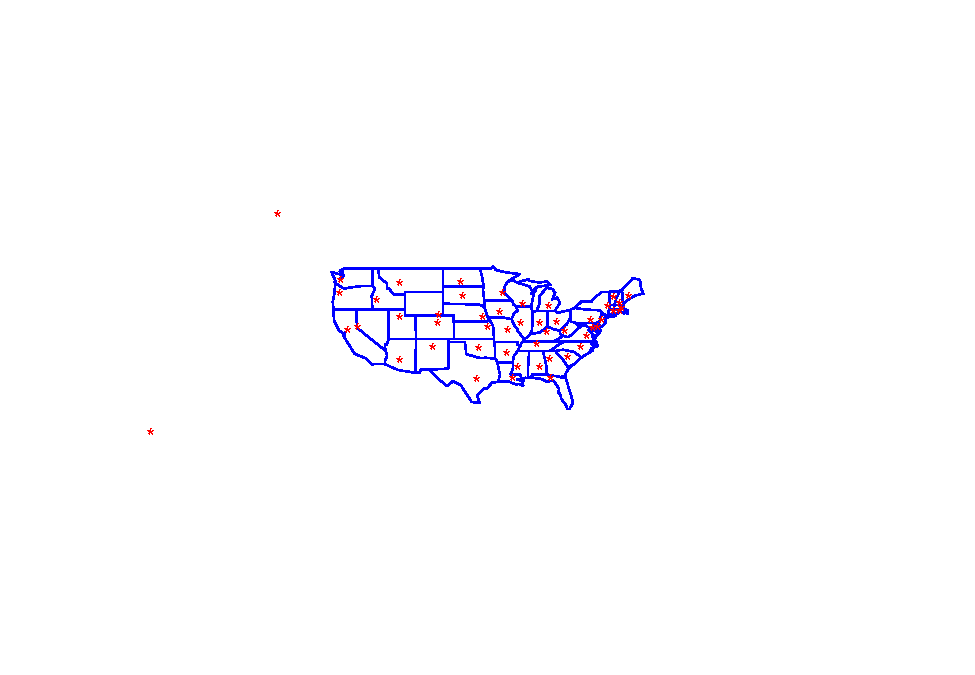
\includegraphics{graphics/chunk-distances-map-base-1.pdf}

\hypertarget{points-comparing-visualization-options}{%
\paragraph{(5 points) Comparing ``Visualization
Options''}\label{points-comparing-visualization-options}}

Above, the data was displayed using three different visualization
packages.

The first \texttt{plot\_usmap} uses the `\texttt{ggplot2} methodology
which is tied to the ``tidyverse'' landscape of the \texttt{R}
community.

The second \texttt{voronoi.mosaic} uses the graph-theory topology known
as Voroni partitioning
\url{https://en.wikipedia.org/wiki/Voronoi_diagram} with the ``base''
plot function to visualize the topology.

The last one \texttt{map} is from the ``base'' environment.

{[} Visually, which is the most appealing to you? Why?

Functionally, which presents the data most effectively? Why?

When we create visualizations, it is essential to portray the data
accurately. For example, there are times when putting Alaska/Hawaii next
to California might be appropriate, and other times it might not be.

What is a one key factor that would determine this appropriateness?

{]}

\hypertarget{points-building-the-distance-matrix}{%
\paragraph{(5 points) Building the distance
matrix}\label{points-building-the-distance-matrix}}

The dataframe we are using has been named \texttt{latlong} to represent
the latitudes and longitudes of the 50 U.S. cities in America.

\begin{Shaded}
\begin{Highlighting}[]
\CommentTok{\# manual conversion}
\CommentTok{\# how many miles is 1 degree of latitude}
\NormalTok{latitude.factor =}\StringTok{ }\DecValTok{69}\NormalTok{;  }\CommentTok{\# rough mile estimate  \# 68.703 ?}
\NormalTok{latlong}\OperatorTok{$}\NormalTok{x.lat =}\StringTok{ }\NormalTok{latlong}\OperatorTok{$}\NormalTok{latitude }\OperatorTok{*}\StringTok{ }\NormalTok{latitude.factor;}

\NormalTok{longitude.factor =}\StringTok{ }\FloatTok{54.6}\NormalTok{;  }\CommentTok{\# rough mile estimate  }
\NormalTok{latlong}\OperatorTok{$}\NormalTok{y.long =}\StringTok{ }\NormalTok{latlong}\OperatorTok{$}\NormalTok{longitude }\OperatorTok{*}\StringTok{ }\NormalTok{longitude.factor;}

\NormalTok{latlong =}\StringTok{ }\KeywordTok{moveColumnsInDataFrame}\NormalTok{(latlong, }\KeywordTok{c}\NormalTok{(}\StringTok{"y.long"}\NormalTok{,}\StringTok{"x.lat"}\NormalTok{), }\StringTok{"before"}\NormalTok{, }\StringTok{"longitude"}\NormalTok{);}
\end{Highlighting}
\end{Shaded}

Let's start with geo-spatial distances. I will do \texttt{distMeeus} and
you will do \texttt{distHaversine}

\hypertarget{meeus}{%
\subparagraph{\texorpdfstring{\textbf{Meeus}}{Meeus}}\label{meeus}}

These distance formulas can utilize the true geo-spatial coordinates.
The distance table is getting large, so there is a helper function to
lookup a certain value.

\begin{Shaded}
\begin{Highlighting}[]
\KeywordTok{library}\NormalTok{(geosphere);}
\KeywordTok{library}\NormalTok{(measurements);}


\NormalTok{dist.meeus =}\StringTok{ }\KeywordTok{conv\_unit}\NormalTok{(  }\KeywordTok{distm}\NormalTok{( latlong[,}\DecValTok{3}\OperatorTok{:}\DecValTok{4}\NormalTok{],}
                  \DataTypeTok{fun=}\NormalTok{distMeeus),  }\StringTok{"m"}\NormalTok{, }\StringTok{"mi"}\NormalTok{);  }\CommentTok{\# default meters to miles}

\NormalTok{dist.meeus.m =}\StringTok{ }\KeywordTok{as.matrix}\NormalTok{( dist.meeus );}
  \KeywordTok{rownames}\NormalTok{(dist.meeus.m) =}\StringTok{ }
\StringTok{  }\KeywordTok{colnames}\NormalTok{(dist.meeus.m) =}\StringTok{ }\NormalTok{myLabels;}

\NormalTok{dist.meeus.df =}\StringTok{ }\KeywordTok{as.data.frame}\NormalTok{( }\KeywordTok{round}\NormalTok{( dist.meeus.m, }\DataTypeTok{digits=}\DecValTok{1}\NormalTok{) );}

\NormalTok{dist.meeus.df;  }\CommentTok{\#\# too big}
\end{Highlighting}
\end{Shaded}

\begin{verbatim}
##                    Montgomery, AL Juneau, AK Phoenix, AZ Little Rock, AR
## Montgomery, AL                0.0     2855.6      1497.1           385.6
## Juneau, AK                 2855.6        0.0      2005.8          2516.3
## Phoenix, AZ                1497.1     2005.8         0.0          1133.4
## Little Rock, AR             385.6     2516.3      1133.4             0.0
## Sacramento, CA             2018.8     1480.3       635.1          1634.7
## Denver, CO                 1161.4     1825.6       585.2           777.6
## Hartford, CT                990.5     2855.1      2215.2          1170.3
## Dover, DE                   763.8     2881.2      2062.7           977.2
## Tallahassee, FL             177.7     3032.3      1642.0           555.6
## Atlanta, GA                 145.7     2845.3      1591.5           459.4
## Honolulu, HI               4408.0     2809.0      2910.9          4040.4
## Boise, ID                  1795.1     1280.7       735.9          1413.7
## Springfield, IL             546.4     2338.4      1316.1           379.0
## Indianapolis, IN            510.7     2464.8      1498.7           485.8
## Des Moines, IA              754.3     2106.8      1154.9           478.0
## Topeka, KS                  701.4     2167.1       991.0           351.1
## Frankfort, KY               410.3     2591.8      1556.0           479.2
## Baton Rouge, LA             318.1     2796.7      1242.3           303.1
## Augusta, ME                1213.3     2836.7      2370.3          1367.5
## Annapolis, MD               713.6     2855.0      2010.2           923.1
## Boston, MA                 1081.8     2884.4      2299.3          1261.7
## Lansing, MI                 721.6     2375.7      1621.6           693.0
## Saint Paul, MN              942.1     1961.5      1285.2           705.4
## Jackson, MS                 228.5     2725.0      1272.6           208.7
## Jefferson City, MO          542.0     2313.6      1166.3           265.0
## Helena, MT                 1677.8     1234.8       906.7          1312.5
## Lincoln, NE                 819.6     2040.7       987.5           481.6
## Carson City, NV            1927.5     1474.7       582.6          1542.6
## Concord, NH                1097.1     2826.1      2277.8          1258.1
## Trenton, NJ                 839.5     2855.3      2103.4          1034.8
## Santa Fe, NM               1150.5     2031.7       380.0           773.5
## Albany, NY                  986.3     2772.4      2162.9          1139.4
## Raleigh, NC                 497.2     2943.7      1903.0           777.2
## Bismarck, ND               1257.7     1600.9      1095.9           942.4
## Columbus, OH                555.1     2568.8      1666.8           626.9
## Oklahoma City, OK           680.1     2303.0       841.2           298.3
## Salem, OR                  2146.1     1042.2       985.5          1764.9
## Harrisburg, PA              755.8     2776.0      1991.9           929.3
## Providence, RI             1045.8     2897.5      2279.9          1233.3
## Columbia, SC                324.2     2951.4      1780.7           647.3
## Pierre, SD                 1122.7     1733.9       982.0           789.0
## Nashville, TN               263.8     2630.7      1445.5           328.1
## Austin, TX                  692.9     2596.4       869.6           441.1
## Salt Lake City, UT         1530.8     1564.2       504.3          1145.8
## Montpelier, VT             1105.1     2738.3      2231.8          1238.6
## Richmond, VA                613.7     2893.7      1959.9           852.4
## Olympia, WA                2171.6      914.1      1096.3          1795.8
## Charleston, WV              488.8     2700.6      1732.1           644.7
## Madison, WI                 758.0     2184.2      1394.4           596.6
## Cheyenne, WY               1190.0     1753.3       663.3           811.4
##                    Sacramento, CA Denver, CO Hartford, CT Dover, DE
## Montgomery, AL             2018.8     1161.4        990.5     763.8
## Juneau, AK                 1480.3     1825.6       2855.1    2881.2
## Phoenix, AZ                 635.1      585.2       2215.2    2062.7
## Little Rock, AR            1634.7      777.6       1170.3     977.2
## Sacramento, CA                0.0      888.7       2558.5    2452.1
## Denver, CO                  888.7        0.0       1691.6    1569.4
## Hartford, CT               2558.5     1691.6          0.0     234.2
## Dover, DE                  2452.1     1569.4        234.2       0.0
## Tallahassee, FL            2181.2     1333.2       1011.7     777.8
## Atlanta, GA                2086.5     1211.9        845.0     618.1
## Honolulu, HI               2461.8     3343.9       5018.8    4912.6
## Boise, ID                   443.7      638.1       2194.7    2114.9
## Springfield, IL            1702.3      815.5        899.4     756.0
## Indianapolis, IN           1886.8     1001.0        719.9     569.8
## Des Moines, IA             1485.1      610.4       1081.2     967.7
## Topeka, KS                 1388.2      499.8       1224.4    1081.6
## Frankfort, KY              1975.1     1086.5        691.5     509.2
## Baton Rouge, LA            1808.7     1009.1       1291.6    1071.2
## Augusta, ME                2669.3     1824.8        228.9     463.1
## Annapolis, MD              2404.2     1520.3        278.9      54.1
## Boston, MA                 2631.2     1769.7         92.5     321.7
## Lansing, MI                1946.8     1082.0        612.0     532.2
## Saint Paul, MN             1522.9      706.2       1048.8     985.4
## Jackson, MS                1809.3      973.2       1163.9     948.4
## Jefferson City, MO         1580.7      692.4       1052.8     897.5
## Helena, MT                  733.2      591.0       1962.3    1903.8
## Lincoln, NE                1327.0      445.2       1247.2    1125.8
## Carson City, NV             101.5      790.4       2457.2    2351.7
## Concord, NH                2596.2     1740.9        115.3     348.1
## Trenton, NJ                2474.4     1596.8        152.3      84.0
## Santa Fe, NM                879.6      285.9       1835.3    1683.7
## Albany, NY                 2492.3     1631.0         82.8     258.3
## Raleigh, NC                2351.8     1463.5        523.7     289.6
## Bismarck, ND               1192.5      531.9       1428.7    1377.1
## Columbus, OH               2050.2     1166.5        554.7     402.9
## Oklahoma City, OK          1338.8      504.4       1407.2    1234.8
## Salem, OR                   445.9      988.8       2505.8    2441.0
## Harrisburg, PA             2364.7     1485.9        242.5     105.2
## Providence, RI             2620.9     1755.3         64.8     283.7
## Columbia, SC               2262.0     1380.1        703.1     469.2
## Pierre, SD                 1165.3      399.8       1404.0    1325.0
## Nashville, TN              1906.3     1022.4        850.8     650.3
## Austin, TX                 1467.2      770.9       1603.7    1400.2
## Salt Lake City, UT          533.3      371.5       2025.4    1920.1
## Montpelier, VT             2533.0     1686.2        172.4     383.6
## Richmond, VA               2378.8     1490.9        387.8     153.9
## Olympia, WA                 588.0     1029.5       2469.5    2418.7
## Charleston, WV             2144.4     1256.6        529.9     334.6
## Madison, WI                1700.6      841.4        857.9     771.0
## Cheyenne, WY                902.5       97.1       1659.8    1549.8
##                    Tallahassee, FL Atlanta, GA Honolulu, HI Boise, ID
## Montgomery, AL               177.7       145.7       4408.0    1795.1
## Juneau, AK                  3032.3      2845.3       2809.0    1280.7
## Phoenix, AZ                 1642.0      1591.5       2910.9     735.9
## Little Rock, AR              555.6       459.4       4040.4    1413.7
## Sacramento, CA              2181.2      2086.5       2461.8     443.7
## Denver, CO                  1333.2      1211.9       3343.9     638.1
## Hartford, CT                1011.7       845.0       5018.8    2194.7
## Dover, DE                    777.8       618.1       4912.6    2114.9
## Tallahassee, FL                0.0       227.5       4549.8    1968.8
## Atlanta, GA                  227.5         0.0       4499.8    1835.5
## Honolulu, HI                4549.8      4499.8          0.0    2835.4
## Boise, ID                   1968.8      1835.5       2835.4       0.0
## Springfield, IL              712.8       508.7       4159.3    1391.7
## Indianapolis, IN             651.0       426.1       4344.9    1567.8
## Des Moines, IA               928.6       739.4       3946.6    1156.3
## Topeka, KS                   878.9       727.3       3838.8    1109.0
## Frankfort, KY                535.0       307.6       4426.8    1671.8
## Baton Rouge, LA              413.2       458.6       4142.8    1644.5
## Augusta, ME                 1240.0      1068.5       5118.9    2284.0
## Annapolis, MD                733.8       567.9       4864.0    2070.8
## Boston, MA                  1099.1       936.2       5089.5    2260.7
## Lansing, MI                  846.8       619.3       4407.8    1590.8
## Saint Paul, MN              1108.9       900.5       3975.7    1146.0
## Jackson, MS                  372.8       351.0       4182.9    1611.2
## Jefferson City, MO           718.8       547.3       4029.5    1296.5
## Helena, MT                  1855.1      1696.3       3095.1     289.8
## Lincoln, NE                  997.3       832.4       3786.8    1017.8
## Carson City, NV             2091.5      1992.4       2562.8     358.7
## Concord, NH                 1124.2       952.1       5052.0    2220.3
## Trenton, NJ                  859.6       693.9       4936.2    2126.5
## Santa Fe, NM                1306.9      1232.6       3268.4     772.7
## Albany, NY                  1022.0       842.1       4951.0    2123.3
## Raleigh, NC                  490.0       355.6       4795.1    2055.2
## Bismarck, ND                1433.3      1244.7       3617.5     782.7
## Columbus, OH                 659.2       434.9       4510.0    1721.6
## Oklahoma City, OK            843.7       757.0       3743.7    1141.4
## Salem, OR                   2319.9      2184.7       2560.8     351.2
## Harrisburg, PA               793.9       611.5       4826.3    2020.4
## Providence, RI              1060.3       900.2       5080.7    2254.7
## Columbia, SC                 308.5       193.6       4686.2    1993.1
## Pierre, SD                  1299.9      1123.5       3617.8     792.1
## Nashville, TN                419.9       214.7       4340.3    1635.7
## Austin, TX                   805.4       819.2       3755.2    1369.4
## Salt Lake City, UT          1701.0      1583.4       2995.0     296.2
## Montpelier, VT              1146.1       962.0       4984.9    2150.9
## Richmond, VA                 623.9       468.4       4833.2    2061.3
## Olympia, WA                 2347.5      2200.4       2636.9     402.7
## Charleston, WV               564.1       352.2       4599.2    1830.1
## Madison, WI                  915.1       697.3       4161.3    1345.8
## Cheyenne, WY                1364.7      1229.4       3364.0     606.4
##                    Springfield, IL Indianapolis, IN Des Moines, IA Topeka, KS
## Montgomery, AL               546.4            510.7          754.3      701.4
## Juneau, AK                  2338.4           2464.8         2106.8     2167.1
## Phoenix, AZ                 1316.1           1498.7         1154.9      991.0
## Little Rock, AR              379.0            485.8          478.0      351.1
## Sacramento, CA              1702.3           1886.8         1485.1     1388.2
## Denver, CO                   815.5           1001.0          610.4      499.8
## Hartford, CT                 899.4            719.9         1081.2     1224.4
## Dover, DE                    756.0            569.8          967.7     1081.6
## Tallahassee, FL              712.8            651.0          928.6      878.9
## Atlanta, GA                  508.7            426.1          739.4      727.3
## Honolulu, HI                4159.3           4344.9         3946.6     3838.8
## Boise, ID                   1391.7           1567.8         1156.3     1109.0
## Springfield, IL                0.0            186.1          242.2      326.8
## Indianapolis, IN             186.1              0.0          411.5      512.2
## Des Moines, IA               242.2            411.5            0.0      206.2
## Topeka, KS                   326.8            512.2          206.2        0.0
## Frankfort, KY                280.3            128.6          520.4      588.2
## Baton Rouge, LA              650.4            702.4          780.3      646.3
## Augusta, ME                 1065.6            897.2         1219.0     1382.2
## Annapolis, MD                705.8            519.7          920.9     1030.7
## Boston, MA                   984.6            807.2         1159.5     1308.2
## Lansing, MI                  334.2            221.1          472.3      635.6
## Saint Paul, MN               396.2            503.3          233.0      427.7
## Jackson, MS                  518.0            562.1          668.2      559.1
## Jefferson City, MO           159.4            333.2          221.6      192.6
## Helena, MT                  1217.7           1381.2          975.7      976.4
## Lincoln, NE                  377.4            560.2          168.3      131.9
## Carson City, NV             1602.8           1787.0         1384.4     1290.2
## Concord, NH                  966.7            793.7         1131.9     1287.4
## Trenton, NJ                  789.6            605.0          989.7     1116.5
## Santa Fe, NM                 936.1           1118.8          781.8      611.5
## Albany, NY                   850.0            675.4         1020.9     1172.1
## Raleigh, NC                  663.7            495.6          902.8      963.7
## Bismarck, ND                 739.6            881.1          505.9      593.9
## Columbus, OH                 353.8            168.4          567.9      680.4
## Oklahoma City, OK            524.4            689.6          472.1      267.2
## Salem, OR                   1732.2           1904.5         1493.6     1457.6
## Harrisburg, PA               677.9            493.4          879.7     1004.8
## Providence, RI               964.2            784.6         1144.9     1289.1
## Columbia, SC                 622.2            488.4          863.6      885.5
## Pierre, SD                   631.9            793.2          389.9      438.0
## Nashville, TN                295.5            250.8          524.9      527.4
## Austin, TX                   800.5            926.1          814.0      617.0
## Salt Lake City, UT          1173.8           1357.0          952.5      867.6
## Montpelier, VT               929.1            763.5         1080.3     1244.2
## Richmond, VA                 676.8            494.5          905.3      994.4
## Olympia, WA                 1731.3           1897.1         1489.9     1474.3
## Charleston, WV               442.6            262.3          673.9      760.6
## Madison, WI                  226.5            283.0          239.9      430.3
## Cheyenne, WY                 803.4            986.3          582.7      504.4
##                    Frankfort, KY Baton Rouge, LA Augusta, ME Annapolis, MD
## Montgomery, AL             410.3           318.1      1213.3         713.6
## Juneau, AK                2591.8          2796.7      2836.7        2855.0
## Phoenix, AZ               1556.0          1242.3      2370.3        2010.2
## Little Rock, AR            479.2           303.1      1367.5         923.1
## Sacramento, CA            1975.1          1808.7      2669.3        2404.2
## Denver, CO                1086.5          1009.1      1824.8        1520.3
## Hartford, CT               691.5          1291.6       228.9         278.9
## Dover, DE                  509.2          1071.2       463.1          54.1
## Tallahassee, FL            535.0           413.2      1240.0         733.8
## Atlanta, GA                307.6           458.6      1068.5         567.9
## Honolulu, HI              4426.8          4142.8      5118.9        4864.0
## Boise, ID                 1671.8          1644.5      2284.0        2070.8
## Springfield, IL            280.3           650.4      1065.6         705.8
## Indianapolis, IN           128.6           702.4       897.2         519.7
## Des Moines, IA             520.4           780.3      1219.0         920.9
## Topeka, KS                 588.2           646.3      1382.2        1030.7
## Frankfort, KY                0.0           644.4       889.8         455.9
## Baton Rouge, LA            644.4             0.0      1508.7        1019.3
## Augusta, ME                889.8          1508.7         0.0         506.4
## Annapolis, MD              455.9          1019.3       506.4           0.0
## Boston, MA                 782.7          1383.8       149.5         368.9
## Lansing, MI                313.3           923.2       748.7         494.7
## Saint Paul, MN             630.5          1005.2      1146.5         946.5
## Jackson, MS                505.7           140.4      1377.8         895.6
## Jefferson City, MO         397.4           563.2      1223.7         845.7
## Helena, MT                1495.5          1576.5      2034.6        1863.4
## Lincoln, NE                655.8           778.1      1387.2        1077.4
## Carson City, NV           1876.4          1724.1      2567.9        2304.0
## Concord, NH                779.3          1393.6       116.4         390.3
## Trenton, NJ                559.5          1143.2       380.4         126.7
## Santa Fe, NM              1178.3           929.1      1992.5        1631.4
## Albany, NY                 660.7          1278.9       230.4         291.8
## Raleigh, NC                383.4           813.8       752.6         250.3
## Bismarck, ND              1003.8          1240.2      1504.1        1338.8
## Columbus, OH               157.6           801.9       741.4         354.1
## Oklahoma City, OK          725.6           505.3      1585.8        1181.3
## Salem, OR                 2012.5          1993.0      2578.2        2398.9
## Harrisburg, PA             451.7          1051.6       458.0          91.7
## Providence, RI             754.8          1349.6       190.7         332.3
## Columbia, SC               360.2           642.2       931.6         425.6
## Pierre, SD                 908.1          1082.3      1504.5        1282.3
## Nashville, TN              175.6           468.9      1057.0         596.3
## Austin, TX                 916.3           392.3      1806.0        1346.5
## Salt Lake City, UT        1449.7          1360.6      2139.8        1872.8
## Montpelier, VT             763.5          1392.4       138.7         417.5
## Richmond, VA               407.1           924.9       616.4         112.4
## Olympia, WA               2010.2          2038.6      2529.0        2378.9
## Charleston, WV             176.1           769.8       740.2         280.9
## Madison, WI                411.6           876.3       983.4         729.3
## Cheyenne, WY              1080.5          1060.8      1782.9        1502.2
##                    Boston, MA Lansing, MI Saint Paul, MN Jackson, MS
## Montgomery, AL         1081.8       721.6          942.1       228.5
## Juneau, AK             2884.4      2375.7         1961.5      2725.0
## Phoenix, AZ            2299.3      1621.6         1285.2      1272.6
## Little Rock, AR        1261.7       693.0          705.4       208.7
## Sacramento, CA         2631.2      1946.8         1522.9      1809.3
## Denver, CO             1769.7      1082.0          706.2       973.2
## Hartford, CT             92.5       612.0         1048.8      1163.9
## Dover, DE               321.7       532.2          985.4       948.4
## Tallahassee, FL        1099.1       846.8         1108.9       372.8
## Atlanta, GA             936.2       619.3          900.5       351.0
## Honolulu, HI           5089.5      4407.8         3975.7      4182.9
## Boise, ID              2260.7      1590.8         1146.0      1611.2
## Springfield, IL         984.6       334.2          396.2       518.0
## Indianapolis, IN        807.2       221.1          503.3       562.1
## Des Moines, IA         1159.5       472.3          233.0       668.2
## Topeka, KS             1308.2       635.6          427.7       559.1
## Frankfort, KY           782.7       313.3          630.5       505.7
## Baton Rouge, LA        1383.8       923.2         1005.2       140.4
## Augusta, ME             149.5       748.7         1146.5      1377.8
## Annapolis, MD           368.9       494.7          946.5       895.6
## Boston, MA                0.0       687.9         1115.1      1256.3
## Lansing, MI             687.9         0.0          453.3       783.0
## Saint Paul, MN         1115.1       453.3            0.0       886.2
## Jackson, MS            1256.3       783.0          886.2         0.0
## Jefferson City, MO     1139.4       492.5          442.0       447.1
## Helena, MT             2022.6      1372.5          919.6      1519.2
## Lincoln, NE            1326.5       640.1          338.5       688.6
## Carson City, NV        2529.8      1845.5         1421.5      1720.4
## Concord, NH              63.4       659.6         1076.4      1263.4
## Trenton, NJ             242.4       536.1          987.5      1017.6
## Santa Fe, NM           1919.6      1244.2          931.6       934.1
## Albany, NY              139.1       549.0          977.4      1147.5
## Raleigh, NC             609.8       575.5          989.1       704.1
## Bismarck, ND           1489.0       844.9          392.5      1147.5
## Columbus, OH            643.5       207.5          619.3       663.3
## Oklahoma City, OK      1495.8       857.2          694.2       474.8
## Salem, OR              2566.7      1911.6         1460.2      1962.0
## Harrisburg, PA          334.9       432.6          885.7       922.4
## Providence, RI           41.2       674.9         1108.7      1223.3
## Columbia, SC            790.7       631.7          990.6       543.0
## Pierre, SD             1472.2       798.7          358.2       996.6
## Nashville, TN           943.0       468.5          690.2       330.1
## Austin, TX             1695.8      1127.9         1043.4       468.5
## Salt Lake City, UT     2098.7      1413.6          994.8      1336.5
## Montpelier, VT          151.8       610.2         1010.6      1258.9
## Richmond, VA            475.6       518.6          958.8       806.3
## Olympia, WA            2526.2      1886.7         1433.5      1997.7
## Charleston, WV          622.2       339.2          746.6       637.7
## Madison, WI             932.0       246.6          225.4       744.5
## Cheyenne, WY           1735.2      1048.0          648.4      1013.4
##                    Jefferson City, MO Helena, MT Lincoln, NE Carson City, NV
## Montgomery, AL                  542.0     1677.8       819.6          1927.5
## Juneau, AK                     2313.6     1234.8      2040.7          1474.7
## Phoenix, AZ                    1166.3      906.7       987.5           582.6
## Little Rock, AR                 265.0     1312.5       481.6          1542.6
## Sacramento, CA                 1580.7      733.2      1327.0           101.5
## Denver, CO                      692.4      591.0       445.2           790.4
## Hartford, CT                   1052.8     1962.3      1247.2          2457.2
## Dover, DE                       897.5     1903.8      1125.8          2351.7
## Tallahassee, FL                 718.8     1855.1       997.3          2091.5
## Atlanta, GA                     547.3     1696.3       832.4          1992.4
## Honolulu, HI                   4029.5     3095.1      3786.8          2562.8
## Boise, ID                      1296.5      289.8      1017.8           358.7
## Springfield, IL                 159.4     1217.7       377.4          1602.8
## Indianapolis, IN                333.2     1381.2       560.2          1787.0
## Des Moines, IA                  221.6      975.7       168.3          1384.4
## Topeka, KS                      192.6      976.4       131.9          1290.2
## Frankfort, KY                   397.4     1495.5       655.8          1876.4
## Baton Rouge, LA                 563.2     1576.5       778.1          1724.1
## Augusta, ME                    1223.7     2034.6      1387.2          2567.9
## Annapolis, MD                   845.7     1863.4      1077.4          2304.0
## Boston, MA                     1139.4     2022.6      1326.5          2529.8
## Lansing, MI                     492.5     1372.5       640.1          1845.5
## Saint Paul, MN                  442.0      919.6       338.5          1421.5
## Jackson, MS                     447.1     1519.2       688.6          1720.4
## Jefferson City, MO                0.0     1149.0       285.2          1482.8
## Helena, MT                     1149.0        0.0       863.9           645.4
## Lincoln, NE                     285.2      863.9         0.0          1227.0
## Carson City, NV                1482.8      645.4      1227.0             0.0
## Concord, NH                    1123.5     1978.5      1299.7          2494.8
## Trenton, NJ                     937.2     1907.0      1151.7          2373.6
## Santa Fe, NM                    786.7      816.7       616.6           795.7
## Albany, NY                     1006.1     1887.5      1188.1          2390.9
## Raleigh, NC                     771.1     1876.3      1038.5          2253.9
## Bismarck, ND                    716.7      533.8       462.1          1093.2
## Columbus, OH                    500.8     1523.6       723.3          1950.0
## Oklahoma City, OK               365.1     1075.1       371.2          1248.1
## Salem, OR                      1643.3      544.2      1362.0           432.6
## Harrisburg, PA                  825.7     1805.1      1040.9          2263.9
## Providence, RI                 1117.6     2020.0      1311.2          2519.5
## Columbia, SC                    696.6     1836.5       978.3          2166.4
## Pierre, SD                      581.5      588.1       308.1          1064.0
## Nashville, TN                   340.0     1486.7       624.2          1810.0
## Austin, TX                      654.8     1361.9       729.2          1390.5
## Salt Lake City, UT             1059.7      402.6       796.9           432.2
## Montpelier, VT                 1087.6     1904.8      1248.5          2431.6
## Richmond, VA                    804.4     1866.2      1053.8          2279.4
## Olympia, WA                    1654.4      516.5      1369.8           566.0
## Charleston, WV                  571.5     1641.4       819.9          2045.1
## Madison, WI                     343.0     1134.2       406.9          1599.3
## Cheyenne, WY                    694.6      520.1       426.2           801.9
##                    Concord, NH Trenton, NJ Santa Fe, NM Albany, NY Raleigh, NC
## Montgomery, AL          1097.1       839.5       1150.5      986.3       497.2
## Juneau, AK              2826.1      2855.3       2031.7     2772.4      2943.7
## Phoenix, AZ             2277.8      2103.4        380.0     2162.9      1903.0
## Little Rock, AR         1258.1      1034.8        773.5     1139.4       777.2
## Sacramento, CA          2596.2      2474.4        879.6     2492.3      2351.8
## Denver, CO              1740.9      1596.8        285.9     1631.0      1463.5
## Hartford, CT             115.3       152.3       1835.3       82.8       523.7
## Dover, DE                348.1        84.0       1683.7      258.3       289.6
## Tallahassee, FL         1124.2       859.6       1306.9     1022.0       490.0
## Atlanta, GA              952.1       693.9       1232.6      842.1       355.6
## Honolulu, HI            5052.0      4936.2       3268.4     4951.0      4795.1
## Boise, ID               2220.3      2126.5        772.7     2123.3      2055.2
## Springfield, IL          966.7       789.6        936.1      850.0       663.7
## Indianapolis, IN         793.7       605.0       1118.8      675.4       495.6
## Des Moines, IA          1131.9       989.7        781.8     1020.9       902.8
## Topeka, KS              1287.4      1116.5        611.5     1172.1       963.7
## Frankfort, KY            779.3       559.5       1178.3      660.7       383.4
## Baton Rouge, LA         1393.6      1143.2        929.1     1278.9       813.8
## Augusta, ME              116.4       380.4       1992.5      230.4       752.6
## Annapolis, MD            390.3       126.7       1631.4      291.8       250.3
## Boston, MA                63.4       242.4       1919.6      139.1       609.8
## Lansing, MI              659.6       536.1       1244.2      549.0       575.5
## Saint Paul, MN          1076.4       987.5        931.6      977.4       989.1
## Jackson, MS             1263.4      1017.6        934.1     1147.5       704.1
## Jefferson City, MO      1123.5       937.2        786.7     1006.1       771.1
## Helena, MT              1978.5      1907.0        816.7     1887.5      1876.3
## Lincoln, NE             1299.7      1151.7        616.6     1188.1      1038.5
## Carson City, NV         2494.8      2373.6        795.7     2390.9      2253.9
## Concord, NH                0.0       264.9       1898.8      118.9       637.6
## Trenton, NJ              264.9         0.0       1723.6      175.6       372.9
## Santa Fe, NM            1898.8      1723.6          0.0     1783.6      1531.7
## Albany, NY               118.9       175.6       1783.6        0.0       542.1
## Raleigh, NC              637.6       372.9       1531.7      542.1         0.0
## Bismarck, ND            1445.4      1376.4        814.4     1353.7      1374.4
## Columbus, OH             634.1       436.7       1287.0      515.2       375.0
## Oklahoma City, OK       1483.3      1283.1        475.6     1365.0      1061.9
## Salem, OR               2522.7      2447.3       1102.1     2431.4      2395.7
## Harrisburg, PA           342.2       111.7       1612.0      230.7       325.0
## Providence, RI            95.6       206.6       1900.1      132.7       570.6
## Columbia, SC             815.8       551.1       1417.8      715.2       182.9
## Pierre, SD              1434.3      1334.6        670.7     1334.0      1288.3
## Nashville, TN            944.5       710.8       1074.6      826.9       457.5
## Austin, TX              1695.2      1463.5        605.0     1576.8      1170.1
## Salt Lake City, UT      2064.6      1941.4        476.7     1959.7      1829.7
## Montpelier, VT            89.3       300.3       1854.2      125.8       667.8
## Richmond, VA             500.9       236.0       1583.5      404.1       137.9
## Olympia, WA             2479.6      2419.7       1174.9     2393.0      2391.8
## Charleston, WV           626.1       390.2       1354.2      509.9       243.2
## Madison, WI              900.5       780.8       1021.6      792.9       763.8
## Cheyenne, WY            1703.4      1572.3        382.6     1596.1      1461.8
##                    Bismarck, ND Columbus, OH Oklahoma City, OK Salem, OR
## Montgomery, AL           1257.7        555.1             680.1    2146.1
## Juneau, AK               1600.9       2568.8            2303.0    1042.2
## Phoenix, AZ              1095.9       1666.8             841.2     985.5
## Little Rock, AR           942.4        626.9             298.3    1764.9
## Sacramento, CA           1192.5       2050.2            1338.8     445.9
## Denver, CO                531.9       1166.5             504.4     988.8
## Hartford, CT             1428.7        554.7            1407.2    2505.8
## Dover, DE                1377.1        402.9            1234.8    2441.0
## Tallahassee, FL          1433.3        659.2             843.7    2319.9
## Atlanta, GA              1244.7        434.9             757.0    2184.7
## Honolulu, HI             3617.5       4510.0            3743.7    2560.8
## Boise, ID                 782.7       1721.6            1141.4     351.2
## Springfield, IL           739.6        353.8             524.4    1732.2
## Indianapolis, IN          881.1        168.4             689.6    1904.5
## Des Moines, IA            505.9        567.9             472.1    1493.6
## Topeka, KS                593.9        680.4             267.2    1457.6
## Frankfort, KY            1003.8        157.6             725.6    2012.5
## Baton Rouge, LA          1240.2        801.9             505.3    1993.0
## Augusta, ME              1504.1        741.4            1585.8    2578.2
## Annapolis, MD            1338.8        354.1            1181.3    2398.9
## Boston, MA               1489.0        643.5            1495.8    2566.7
## Lansing, MI               844.9        207.5             857.2    1911.6
## Saint Paul, MN            392.5        619.3             694.2    1460.2
## Jackson, MS              1147.5        663.3             474.8    1962.0
## Jefferson City, MO        716.7        500.8             365.1    1643.3
## Helena, MT                533.8       1523.6            1075.1     544.2
## Lincoln, NE               462.1        723.3             371.2    1362.0
## Carson City, NV          1093.2       1950.0            1248.1     432.6
## Concord, NH              1445.4        634.1            1483.3    2522.7
## Trenton, NJ              1376.4        436.7            1283.1    2447.3
## Santa Fe, NM              814.4       1287.0             475.6    1102.1
## Albany, NY               1353.7        515.2            1365.0    2431.4
## Raleigh, NC              1374.4        375.0            1061.9    2395.7
## Bismarck, ND                0.0       1009.2             800.6    1077.7
## Columbus, OH             1009.2          0.0             852.5    2053.9
## Oklahoma City, OK         800.6        852.5               0.0    1491.2
## Salem, OR                1077.7       2053.9            1491.2       0.0
## Harrisburg, PA           1276.6        325.1            1173.2    2343.8
## Providence, RI           1486.3        619.2            1471.7    2563.8
## Columbia, SC             1359.1        425.2             942.5    2339.6
## Pierre, SD                169.7        937.8             631.9    1116.8
## Nashville, TN            1030.0        333.2             604.6    1983.1
## Austin, TX               1152.6       1067.1             358.7    1705.6
## Salt Lake City, UT        693.9       1518.9             862.5     634.7
## Montpelier, VT           1372.8        611.7            1450.7    2448.9
## Richmond, VA             1350.2        342.6            1123.3    2395.5
## Olympia, WA              1043.4       2040.1            1533.7     145.1
## Charleston, WV           1133.7        133.4             900.7    2166.6
## Madison, WI               614.9        394.5             681.7    1670.0
## Cheyenne, WY              439.9       1148.3             556.7     956.7
##                    Harrisburg, PA Providence, RI Columbia, SC Pierre, SD
## Montgomery, AL              755.8         1045.8        324.2     1122.7
## Juneau, AK                 2776.0         2897.5       2951.4     1733.9
## Phoenix, AZ                1991.9         2279.9       1780.7      982.0
## Little Rock, AR             929.3         1233.3        647.3      789.0
## Sacramento, CA             2364.7         2620.9       2262.0     1165.3
## Denver, CO                 1485.9         1755.3       1380.1      399.8
## Hartford, CT                242.5           64.8        703.1     1404.0
## Dover, DE                   105.2          283.7        469.2     1325.0
## Tallahassee, FL             793.9         1060.3        308.5     1299.9
## Atlanta, GA                 611.5          900.2        193.6     1123.5
## Honolulu, HI               4826.3         5080.7       4686.2     3617.8
## Boise, ID                  2020.4         2254.7       1993.1      792.1
## Springfield, IL             677.9          964.2        622.2      631.9
## Indianapolis, IN            493.4          784.6        488.4      793.2
## Des Moines, IA              879.7         1144.9        863.6      389.9
## Topeka, KS                 1004.8         1289.1        885.5      438.0
## Frankfort, KY               451.7          754.8        360.2      908.1
## Baton Rouge, LA            1051.6         1349.6        642.2     1082.3
## Augusta, ME                 458.0          190.7        931.6     1504.5
## Annapolis, MD                91.7          332.3        425.6     1282.3
## Boston, MA                  334.9           41.2        790.7     1472.2
## Lansing, MI                 432.6          674.9        631.7      798.7
## Saint Paul, MN              885.7         1108.7        990.6      358.2
## Jackson, MS                 922.4         1223.3        543.0      996.6
## Jefferson City, MO          825.7         1117.6        696.6      581.5
## Helena, MT                 1805.1         2020.0       1836.5      588.1
## Lincoln, NE                1040.9         1311.2        978.3      308.1
## Carson City, NV            2263.9         2519.5       2166.4     1064.0
## Concord, NH                 342.2           95.6        815.8     1434.3
## Trenton, NJ                 111.7          206.6        551.1     1334.6
## Santa Fe, NM               1612.0         1900.1       1417.8      670.7
## Albany, NY                  230.7          132.7        715.2     1334.0
## Raleigh, NC                 325.0          570.6        182.9     1288.3
## Bismarck, ND               1276.6         1486.3       1359.1      169.7
## Columbus, OH                325.1          619.2        425.2      937.8
## Oklahoma City, OK          1173.2         1471.7        942.5      631.9
## Salem, OR                  2343.8         2563.8       2339.6     1116.8
## Harrisburg, PA                0.0          304.3        489.4     1229.2
## Providence, RI              304.3            0.0        752.0     1464.7
## Columbia, SC                489.4          752.0          0.0     1253.4
## Pierre, SD                 1229.2         1464.7       1253.4        0.0
## Nashville, TN               608.4          912.6        358.3      910.3
## Austin, TX                 1361.4         1665.6       1011.5      982.9
## Salt Lake City, UT         1831.9         2087.9       1750.9      640.1
## Montpelier, VT              352.6          178.0        840.0     1368.7
## Richmond, VA                191.5          437.3        315.4     1280.0
## Olympia, WA                2319.1         2525.7       2347.0     1104.0
## Charleston, WV              287.4          591.4        301.6     1053.7
## Madison, WI                 674.8          920.4        771.4      554.4
## Cheyenne, WY               1462.3         1722.9       1389.9      319.6
##                    Nashville, TN Austin, TX Salt Lake City, UT Montpelier, VT
## Montgomery, AL             263.8      692.9             1530.8         1105.1
## Juneau, AK                2630.7     2596.4             1564.2         2738.3
## Phoenix, AZ               1445.5      869.6              504.3         2231.8
## Little Rock, AR            328.1      441.1             1145.8         1238.6
## Sacramento, CA            1906.3     1467.2              533.3         2533.0
## Denver, CO                1022.4      770.9              371.5         1686.2
## Hartford, CT               850.8     1603.7             2025.4          172.4
## Dover, DE                  650.3     1400.2             1920.1          383.6
## Tallahassee, FL            419.9      805.4             1701.0         1146.1
## Atlanta, GA                214.7      819.2             1583.4          962.0
## Honolulu, HI              4340.3     3755.2             2995.0         4984.9
## Boise, ID                 1635.7     1369.4              296.2         2150.9
## Springfield, IL            295.5      800.5             1173.8          929.1
## Indianapolis, IN           250.8      926.1             1357.0          763.5
## Des Moines, IA             524.9      814.0              952.5         1080.3
## Topeka, KS                 527.4      617.0              867.6         1244.2
## Frankfort, KY              175.6      916.3             1449.7          763.5
## Baton Rouge, LA            468.9      392.3             1360.6         1392.4
## Augusta, ME               1057.0     1806.0             2139.8          138.7
## Annapolis, MD              596.3     1346.5             1872.8          417.5
## Boston, MA                 943.0     1695.8             2098.7          151.8
## Lansing, MI                468.5     1127.9             1413.6          610.2
## Saint Paul, MN             690.2     1043.4              994.8         1010.6
## Jackson, MS                330.1      468.5             1336.5         1258.9
## Jefferson City, MO         340.0      654.8             1059.7         1087.6
## Helena, MT                1486.7     1361.9              402.6         1904.8
## Lincoln, NE                624.2      729.2              796.9         1248.5
## Carson City, NV           1810.0     1390.5              432.2         2431.6
## Concord, NH                944.5     1695.2             2064.6           89.3
## Trenton, NJ                710.8     1463.5             1941.4          300.3
## Santa Fe, NM              1074.6      605.0              476.7         1854.2
## Albany, NY                 826.9     1576.8             1959.7          125.8
## Raleigh, NC                457.5     1170.1             1829.7          667.8
## Bismarck, ND              1030.0     1152.6              693.9         1372.8
## Columbus, OH               333.2     1067.1             1518.9          611.7
## Oklahoma City, OK          604.6      358.7              862.5         1450.7
## Salem, OR                 1983.1     1705.6              634.7         2448.9
## Harrisburg, PA             608.4     1361.4             1831.9          352.6
## Providence, RI             912.6     1665.6             2087.9          178.0
## Columbia, SC               358.3     1011.5             1750.9          840.0
## Pierre, SD                 910.3      982.9              640.1         1368.7
## Nashville, TN                0.0      753.1             1392.8          934.0
## Austin, TX                 753.1        0.0             1074.1         1678.6
## Salt Lake City, UT        1392.8     1074.1                0.0         2002.8
## Montpelier, VT             934.0     1678.6             2002.8            0.0
## Richmond, VA               524.6     1264.9             1850.5          529.9
## Olympia, WA               1993.9     1771.8              698.8         2402.9
## Charleston, WV             321.2     1074.3             1616.4          622.7
## Madison, WI                496.3      996.5             1167.5          844.8
## Cheyenne, WY              1031.8      848.0              370.8         1645.0
##                    Richmond, VA Olympia, WA Charleston, WV Madison, WI
## Montgomery, AL            613.7      2171.6          488.8       758.0
## Juneau, AK               2893.7       914.1         2700.6      2184.2
## Phoenix, AZ              1959.9      1096.3         1732.1      1394.4
## Little Rock, AR           852.4      1795.8          644.7       596.6
## Sacramento, CA           2378.8       588.0         2144.4      1700.6
## Denver, CO               1490.9      1029.5         1256.6       841.4
## Hartford, CT              387.8      2469.5          529.9       857.9
## Dover, DE                 153.9      2418.7          334.6       771.0
## Tallahassee, FL           623.9      2347.5          564.1       915.1
## Atlanta, GA               468.4      2200.4          352.2       697.3
## Honolulu, HI             4833.2      2636.9         4599.2      4161.3
## Boise, ID                2061.3       402.7         1830.1      1345.8
## Springfield, IL           676.8      1731.3          442.6       226.5
## Indianapolis, IN          494.5      1897.1          262.3       283.0
## Des Moines, IA            905.3      1489.9          673.9       239.9
## Topeka, KS                994.4      1474.3          760.6       430.3
## Frankfort, KY             407.1      2010.2          176.1       411.6
## Baton Rouge, LA           924.9      2038.6          769.8       876.3
## Augusta, ME               616.4      2529.0          740.2       983.4
## Annapolis, MD             112.4      2378.9          280.9       729.3
## Boston, MA                475.6      2526.2          622.2       932.0
## Lansing, MI               518.6      1886.7          339.2       246.6
## Saint Paul, MN            958.8      1433.5          746.6       225.4
## Jackson, MS               806.3      1997.7          637.7       744.5
## Jefferson City, MO        804.4      1654.4          571.5       343.0
## Helena, MT               1866.2       516.5         1641.4      1134.2
## Lincoln, NE              1053.8      1369.8          819.9       406.9
## Carson City, NV          2279.4       566.0         2045.1      1599.3
## Concord, NH               500.9      2479.6          626.1       900.5
## Trenton, NJ               236.0      2419.7          390.2       780.8
## Santa Fe, NM             1583.5      1174.9         1354.2      1021.6
## Albany, NY                404.1      2393.0          509.9       792.9
## Raleigh, NC               137.9      2391.8          243.2       763.8
## Bismarck, ND             1350.2      1043.4         1133.7       614.9
## Columbus, OH              342.6      2040.1          133.4       394.5
## Oklahoma City, OK        1123.3      1533.7          900.7       681.7
## Salem, OR                2395.5       145.1         2166.6      1670.0
## Harrisburg, PA            191.5      2319.1          287.4       674.8
## Providence, RI            437.3      2525.7          591.4       920.4
## Columbia, SC              315.4      2347.0          301.6       771.4
## Pierre, SD               1280.0      1104.0         1053.7       554.4
## Nashville, TN             524.6      1993.9          321.2       496.3
## Austin, TX               1264.9      1771.8         1074.3       996.5
## Salt Lake City, UT       1850.5       698.8         1616.4      1167.5
## Montpelier, VT            529.9      2402.9          622.7       844.8
## Richmond, VA                0.0      2382.7          234.4       735.5
## Olympia, WA              2382.7         0.0         2157.7      1650.1
## Charleston, WV            234.4      2157.7            0.0       521.2
## Madison, WI               735.5      1650.1          521.2         0.0
## Cheyenne, WY             1480.0       984.6         1246.1       803.3
##                    Cheyenne, WY
## Montgomery, AL           1190.0
## Juneau, AK               1753.3
## Phoenix, AZ               663.3
## Little Rock, AR           811.4
## Sacramento, CA            902.5
## Denver, CO                 97.1
## Hartford, CT             1659.8
## Dover, DE                1549.8
## Tallahassee, FL          1364.7
## Atlanta, GA              1229.4
## Honolulu, HI             3364.0
## Boise, ID                 606.4
## Springfield, IL           803.4
## Indianapolis, IN          986.3
## Des Moines, IA            582.7
## Topeka, KS                504.4
## Frankfort, KY            1080.5
## Baton Rouge, LA          1060.8
## Augusta, ME              1782.9
## Annapolis, MD            1502.2
## Boston, MA               1735.2
## Lansing, MI              1048.0
## Saint Paul, MN            648.4
## Jackson, MS              1013.4
## Jefferson City, MO        694.6
## Helena, MT                520.1
## Lincoln, NE               426.2
## Carson City, NV           801.9
## Concord, NH              1703.4
## Trenton, NJ              1572.3
## Santa Fe, NM              382.6
## Albany, NY               1596.1
## Raleigh, NC              1461.8
## Bismarck, ND              439.9
## Columbus, OH             1148.3
## Oklahoma City, OK         556.7
## Salem, OR                 956.7
## Harrisburg, PA           1462.3
## Providence, RI           1722.9
## Columbia, SC             1389.9
## Pierre, SD                319.6
## Nashville, TN            1031.8
## Austin, TX                848.0
## Salt Lake City, UT        370.8
## Montpelier, VT           1645.0
## Richmond, VA             1480.0
## Olympia, WA               984.6
## Charleston, WV           1246.1
## Madison, WI               803.3
## Cheyenne, WY                0.0
\end{verbatim}

\begin{Shaded}
\begin{Highlighting}[]
\KeywordTok{lookupPairwiseValue}\NormalTok{(dist.meeus.df, }\StringTok{"Juneau, AK"}\NormalTok{, }\StringTok{"Montgomery, AL"}\NormalTok{);}
\end{Highlighting}
\end{Shaded}

\begin{verbatim}
## [1] 2855.6
\end{verbatim}

\hypertarget{haversine}{%
\subparagraph{\texorpdfstring{\textbf{Haversine}}{Haversine}}\label{haversine}}

You can compare the two with the code below (currently in comments).

\begin{Shaded}
\begin{Highlighting}[]
\CommentTok{\# }
\CommentTok{\# x = dist.meeus.df[,2]; \# Juneau ... pick one location}
\CommentTok{\# y = dist.haversine.df[,2];}
\CommentTok{\# }
\CommentTok{\# my.lim = c(0, 4000 );}
\CommentTok{\# }
\CommentTok{\# plot(x, y,  }
\CommentTok{\#             xlab="Meeus", }
\CommentTok{\#             ylab="Haversine", }
\CommentTok{\#             main="dist( Juneau, AK )",}
\CommentTok{\#             xlim=my.lim, }
\CommentTok{\#             ylim=my.lim);}
\CommentTok{\# }
\CommentTok{\# plotXYwithBoxPlots(x, y,  }
\CommentTok{\#             xlab="Meeus", }
\CommentTok{\#             ylab="Haversine", }
\CommentTok{\#             main="dist( Juneau, AK )",}
\CommentTok{\#             xlim=my.lim, }
\CommentTok{\#             ylim=my.lim);}
\end{Highlighting}
\end{Shaded}

{[} Examining the data above, is there much difference between these two
calculations?

What is the conceptual difference between these two calculations? Try
\texttt{?distMeeus} or \texttt{?distHaversine}

Are the results similar?

Is there a more accurate distance algorithm for geo-spatial
calculations? If so, what is it?

{]}

Let's now do \texttt{manhattan} and \texttt{euclidean} which are more
common in the ``statistical clustering'' domain. I will do
\texttt{euclidean}.

\hypertarget{manhattan}{%
\subparagraph{\texorpdfstring{\textbf{Manhattan}}{Manhattan}}\label{manhattan}}

\hypertarget{euclidean}{%
\subparagraph{\texorpdfstring{\textbf{Euclidean}}{Euclidean}}\label{euclidean}}

We have converted the true latitude/longitude to a miles-type format, so
the resulting table will report miles.

\begin{Shaded}
\begin{Highlighting}[]
\NormalTok{dist.euclidean =}\StringTok{ }\KeywordTok{dist}\NormalTok{( latlong[,}\DecValTok{1}\OperatorTok{:}\DecValTok{2}\NormalTok{],}
                      \DataTypeTok{method=}\StringTok{"euclidean"}\NormalTok{, }\DataTypeTok{diag=}\OtherTok{TRUE}\NormalTok{, }\DataTypeTok{upper=}\OtherTok{TRUE}\NormalTok{);}
\NormalTok{dist.euclidean.m =}\StringTok{ }\KeywordTok{as.matrix}\NormalTok{( dist.euclidean );}
  \KeywordTok{rownames}\NormalTok{(dist.euclidean.m) =}\StringTok{ }
\StringTok{  }\KeywordTok{colnames}\NormalTok{(dist.euclidean.m) =}\StringTok{ }\NormalTok{myLabels;}

\NormalTok{dist.euclidean.df =}\StringTok{ }\KeywordTok{as.data.frame}\NormalTok{( }\KeywordTok{round}\NormalTok{( dist.euclidean.m, }\DataTypeTok{digits=}\DecValTok{1}\NormalTok{) );}

\NormalTok{dist.euclidean.df;  }\CommentTok{\#\# too big}
\end{Highlighting}
\end{Shaded}

\begin{verbatim}
##                    Montgomery, AL Juneau, AK Phoenix, AZ Little Rock, AR
## Montgomery, AL                0.0     3179.8      1410.0           368.8
## Juneau, AK                 3179.8        0.0      2104.5          2814.9
## Phoenix, AZ                1410.0     2104.5         0.0          1081.2
## Little Rock, AR             368.8     2814.9      1081.2             0.0
## Sacramento, CA             1970.1     1532.6       624.8          1614.3
## Denver, CO                 1141.4     2054.6       581.0           772.6
## Hartford, CT                986.2     3559.0      2226.0          1177.7
## Dover, DE                   751.5     3476.2      2033.7           967.0
## Tallahassee, FL             171.9     3345.6      1532.6           530.8
## Atlanta, GA                 141.0     3213.9      1511.3           438.8
## Honolulu, HI               3982.0     2855.5      2636.9          3695.8
## Boise, ID                  1808.9     1419.7       736.9          1440.2
## Springfield, IL             545.3     2757.3      1299.8           378.7
## Indianapolis, IN            511.1     2928.8      1480.3           483.9
## Des Moines, IA              752.5     2508.1      1153.2           478.2
## Topeka, KS                  690.9     2496.8       974.3           349.9
## Frankfort, KY               410.2     3040.2      1520.9           472.5
## Baton Rouge, LA             298.3     3044.1      1159.2           302.5
## Augusta, ME                1221.2     3658.8      2427.5          1397.4
## Annapolis, MD               702.2     3431.8      1978.9           912.4
## Boston, MA                 1079.8     3629.7      2321.6          1274.7
## Lansing, MI                 721.9     2927.1      1633.5           696.5
## Saint Paul, MN              944.6     2437.2      1304.7           705.6
## Jackson, MS                 213.3     3008.5      1197.4           205.0
## Jefferson City, MO          536.2     2678.0      1142.3           265.1
## Helena, MT                 1714.4     1465.6       906.7          1350.9
## Lincoln, NE                 813.7     2387.9       981.7           481.6
## Carson City, NV            1887.7     1543.7       576.4          1528.8
## Concord, NH                1099.0     3587.6      2313.0          1276.9
## Trenton, NJ                 830.4     3487.7      2089.7          1031.2
## Santa Fe, NM               1098.7     2202.7       366.6           747.1
## Albany, NY                  985.7     3483.5      2186.0          1151.9
## Raleigh, NC                 479.1     3419.6      1832.5           751.3
## Bismarck, ND               1273.1     2000.2      1108.7           952.3
## Columbus, OH                554.1     3079.3      1649.4           624.2
## Oklahoma City, OK           650.2     2557.3       806.3           287.9
## Salem, OR                  2186.7     1111.6       993.7          1818.5
## Harrisburg, PA              749.2     3379.1      1978.2           926.2
## Providence, RI             1041.3     3622.5      2293.2          1242.0
## Columbia, SC                307.9     3362.5      1694.8           618.9
## Pierre, SD                 1129.0     2095.0       989.6           795.2
## Nashville, TN               264.0     3016.0      1393.2           318.6
## Austin, TX                  642.4     2784.0       812.3           427.1
## Salt Lake City, UT         1513.7     1725.4       504.5          1146.0
## Montpelier, VT             1110.7     3512.7      2281.6          1263.0
## Richmond, VA                599.0     3423.7      1910.1           834.2
## Olympia, WA                2241.3      999.6      1108.6          1872.5
## Charleston, WV              484.7     3193.9      1695.7           635.0
## Madison, WI                 758.4     2673.8      1405.3           597.4
## Cheyenne, WY               1179.7     2003.3       661.9           812.6
##                    Sacramento, CA Denver, CO Hartford, CT Dover, DE
## Montgomery, AL             1970.1     1141.4        986.2     751.5
## Juneau, AK                 1532.6     2054.6       3559.0    3476.2
## Phoenix, AZ                 624.8      581.0       2226.0    2033.7
## Little Rock, AR            1614.3      772.6       1177.7     967.0
## Sacramento, CA                0.0      904.7       2674.6    2510.3
## Denver, CO                  904.7        0.0       1770.0    1609.3
## Hartford, CT               2674.6     1770.0          0.0     237.7
## Dover, DE                  2510.3     1609.3        237.7       0.0
## Tallahassee, FL            2109.3     1300.9       1004.2     766.7
## Atlanta, GA                2053.1     1198.2        845.3     611.0
## Honolulu, HI               2315.8     3154.4       4860.5    4661.1
## Boise, ID                   451.9      668.0       2380.0    2242.2
## Springfield, IL            1740.5      837.3        937.0     772.8
## Indianapolis, IN           1931.1     1028.2        749.0     582.1
## Des Moines, IA             1536.0      633.8       1143.7    1002.2
## Topeka, KS                 1409.3      510.0       1270.4    1101.0
## Frankfort, KY              2000.0     1103.9        709.7     514.4
## Baton Rouge, LA            1747.8      989.8       1276.8    1044.9
## Augusta, ME                2851.2     1948.2        236.4     474.1
## Annapolis, MD              2456.8     1556.4        284.1      54.8
## Boston, MA                 2765.8     1861.2         97.1     328.7
## Lansing, MI                2037.6     1135.2        651.7     550.9
## Saint Paul, MN             1611.6      742.2       1136.3    1039.0
## Jackson, MS                1763.6      957.6       1157.8     929.9
## Jefferson City, MO         1600.9      704.4       1087.1     909.9
## Helena, MT                  757.0      609.0       2174.0    2057.6
## Lincoln, NE                1363.6      459.8       1312.3    1160.6
## Carson City, NV             102.5      807.8       2577.5    2415.6
## Concord, NH                2746.2     1842.1        117.4     354.1
## Trenton, NJ                2554.0     1650.7        155.8      84.5
## Santa Fe, NM                871.5      286.0       1865.7    1679.4
## Albany, NY                 2621.5     1717.1         85.3     259.7
## Raleigh, NC                2348.3     1465.0        526.3     289.1
## Bismarck, ND               1265.3      539.1       1573.8    1476.7
## Columbus, OH               2103.9     1200.7        577.3     412.0
## Oklahoma City, OK          1326.4      503.1       1424.5    1227.7
## Salem, OR                   446.7     1048.8       2758.7    2624.8
## Harrisburg, PA             2439.0     1535.5        251.5     106.4
## Providence, RI             2743.1     1838.5         68.5     289.8
## Columbia, SC               2231.6     1366.6        703.7     466.0
## Pierre, SD                 1223.2      408.9       1520.2    1400.8
## Nashville, TN              1902.5     1024.2        861.7     648.5
## Austin, TX                 1418.1      764.0       1582.0    1359.4
## Salt Lake City, UT          545.5      383.3       2142.4    1988.7
## Montpelier, VT             2699.5     1797.1        172.4     387.1
## Richmond, VA               2405.0     1510.5        392.0     154.3
## Olympia, WA                 588.5     1100.0       2766.4    2643.3
## Charleston, WV             2176.5     1278.9        543.0     338.2
## Madison, WI                1780.4      882.6        916.8     803.5
## Cheyenne, WY                927.4       97.1       1755.7    1605.4
##                    Tallahassee, FL Atlanta, GA Honolulu, HI Boise, ID
## Montgomery, AL               171.9       141.0       3982.0    1808.9
## Juneau, AK                  3345.6      3213.9       2855.5    1419.7
## Phoenix, AZ                 1532.6      1511.3       2636.9     736.9
## Little Rock, AR              530.8       438.8       3695.8    1440.2
## Sacramento, CA              2109.3      2053.1       2315.8     451.9
## Denver, CO                  1300.9      1198.2       3154.4     668.0
## Hartford, CT                1004.2       845.3       4860.5    2380.0
## Dover, DE                    766.7       611.0       4661.1    2242.2
## Tallahassee, FL                0.0       227.8       4068.1    1966.6
## Atlanta, GA                  227.8         0.0       4102.3    1865.4
## Honolulu, HI                4068.1      4102.3          0.0    2746.4
## Boise, ID                   1966.6      1865.4       2746.4       0.0
## Springfield, IL              709.0       506.5       3936.4    1473.2
## Indianapolis, IN             651.0       426.0       4116.9    1661.7
## Des Moines, IA               923.0       739.2       3776.3    1240.8
## Topeka, KS                   861.4       717.2       3608.6    1163.3
## Frankfort, KY                535.5       307.8       4152.3    1751.2
## Baton Rouge, LA              378.1       435.3       3694.9    1640.8
## Augusta, ME                 1240.4      1080.2       5064.3    2535.1
## Annapolis, MD                724.3       561.4       4606.3    2191.2
## Boston, MA                  1092.3       939.0       4956.6    2466.1
## Lansing, MI                  847.4       619.6       4267.1    1729.4
## Saint Paul, MN              1110.2       906.6       3894.2    1265.0
## Jackson, MS                  347.9       332.0       3772.0    1621.0
## Jefferson City, MO           707.9       539.7       3779.2    1357.2
## Helena, MT                  1881.0      1749.4       3050.8     307.0
## Lincoln, NE                  985.2       828.9       3601.2    1083.4
## Carson City, NV             2030.0      1967.3       2417.4     363.6
## Concord, NH                 1120.8       958.0       4949.4    2438.8
## Trenton, NJ                  850.2       689.6       4721.0    2274.6
## Santa Fe, NM                1238.8      1185.3       3001.7     783.1
## Albany, NY                  1018.2       845.0       4822.3    2318.4
## Raleigh, NC                  478.0       343.6       4439.3    2121.5
## Bismarck, ND                1444.9      1269.8       3578.7     870.2
## Columbus, OH                 659.6       435.0       4285.1    1830.2
## Oklahoma City, OK            802.8       726.7       3436.3    1164.6
## Salem, OR                   2341.7      2246.9       2504.6     384.3
## Harrisburg, PA               788.0       608.6       4611.2    2159.6
## Providence, RI              1051.7       900.7       4927.2    2448.1
## Columbia, SC                 301.2       184.0       4285.0    2031.5
## Pierre, SD                  1300.7      1137.2       3521.7     868.7
## Nashville, TN                417.6       211.6       4013.9    1686.5
## Austin, TX                   736.7       767.8       3340.0    1365.3
## Salt Lake City, UT          1668.2      1577.5       2846.2     306.9
## Montpelier, VT              1146.2       970.3       4918.4    2382.4
## Richmond, VA                 613.0       459.2       4529.9    2156.2
## Olympia, WA                 2400.4      2293.8       2606.8     435.4
## Charleston, WV               563.0       350.8       4324.8    1922.1
## Madison, WI                  914.7       698.5       4029.1    1464.7
## Cheyenne, WY                1343.3      1226.4       3202.9     644.5
##                    Springfield, IL Indianapolis, IN Des Moines, IA Topeka, KS
## Montgomery, AL               545.3            511.1          752.5      690.9
## Juneau, AK                  2757.3           2928.8         2508.1     2496.8
## Phoenix, AZ                 1299.8           1480.3         1153.2      974.3
## Little Rock, AR              378.7            483.9          478.2      349.9
## Sacramento, CA              1740.5           1931.1         1536.0     1409.3
## Denver, CO                   837.3           1028.2          633.8      510.0
## Hartford, CT                 937.0            749.0         1143.7     1270.4
## Dover, DE                    772.8            582.1         1002.2     1101.0
## Tallahassee, FL              709.0            651.0          923.0      861.4
## Atlanta, GA                  506.5            426.0          739.2      717.2
## Honolulu, HI                3936.4           4116.9         3776.3     3608.6
## Boise, ID                   1473.2           1661.7         1240.8     1163.3
## Springfield, IL                0.0            190.9          249.3      333.5
## Indianapolis, IN             190.9              0.0          426.4      522.7
## Des Moines, IA               249.3            426.4            0.0      208.2
## Topeka, KS                   333.5            522.7          208.2        0.0
## Frankfort, KY                283.8            129.2          532.2      593.8
## Baton Rouge, LA              650.6            699.1          780.4      643.0
## Augusta, ME                 1129.0            947.6         1315.2     1460.4
## Annapolis, MD                720.5            530.1          952.0     1047.7
## Boston, MA                  1030.3            843.3         1232.8     1363.7
## Lansing, MI                  344.6            222.7          501.7      659.2
## Saint Paul, MN               401.6            520.5          233.2      430.3
## Jackson, MS                  518.3            560.3          668.0      554.7
## Jefferson City, MO           161.3            338.6          222.5      194.8
## Helena, MT                  1308.0           1488.5         1062.2     1032.2
## Lincoln, NE                  389.8            578.9          175.5      132.5
## Carson City, NV             1644.7           1835.5         1437.4     1314.7
## Concord, NH                 1016.7            832.8         1210.9     1349.4
## Trenton, NJ                  813.6            622.9         1033.9     1145.4
## Santa Fe, NM                 935.0           1117.8          788.2      607.8
## Albany, NY                   890.1            705.7         1087.0     1222.9
## Raleigh, NC                  663.0            495.0          911.7      958.5
## Bismarck, ND                 776.6            934.7          531.6      602.9
## Columbus, OH                 363.5            172.9          590.7      695.6
## Oklahoma City, OK            523.2            687.7          473.1      267.0
## Salem, OR                   1857.0           2045.1         1622.8     1547.5
## Harrisburg, PA               698.5            508.0          918.8     1030.6
## Providence, RI              1005.3            817.0         1212.2     1338.7
## Columbia, SC                 617.8            486.5          864.0      872.9
## Pierre, SD                   662.3            836.0          413.1      445.5
## Nashville, TN                295.7            250.9          528.6      525.6
## Austin, TX                   792.2            911.0          813.1      616.7
## Salt Lake City, UT          1215.9           1406.7          999.2      892.4
## Montpelier, VT               982.0            803.7         1163.7     1312.1
## Richmond, VA                 683.6            499.0          925.4     1000.5
## Olympia, WA                 1882.7           2067.9         1642.3     1584.5
## Charleston, WV               449.3            265.8          691.7      769.0
## Madison, WI                  226.5            288.2          253.0      442.1
## Cheyenne, WY                 833.2           1023.3          612.3      518.9
##                    Frankfort, KY Baton Rouge, LA Augusta, ME Annapolis, MD
## Montgomery, AL             410.2           298.3      1221.2         702.2
## Juneau, AK                3040.2          3044.1      3658.8        3431.8
## Phoenix, AZ               1520.9          1159.2      2427.5        1978.9
## Little Rock, AR            472.5           302.5      1397.4         912.4
## Sacramento, CA            2000.0          1747.8      2851.2        2456.8
## Denver, CO                1103.9           989.8      1948.2        1556.4
## Hartford, CT               709.7          1276.8       236.4         284.1
## Dover, DE                  514.4          1044.9       474.1          54.8
## Tallahassee, FL            535.5           378.1      1240.4         724.3
## Atlanta, GA                307.8           435.3      1080.2         561.4
## Honolulu, HI              4152.3          3694.9      5064.3        4606.3
## Boise, ID                 1751.2          1640.8      2535.1        2191.2
## Springfield, IL            283.8           650.6      1129.0         720.5
## Indianapolis, IN           129.2           699.1       947.6         530.1
## Des Moines, IA             532.2           780.4      1315.2         952.0
## Topeka, KS                 593.8           643.0      1460.4        1047.7
## Frankfort, KY                0.0           636.3       925.4         459.9
## Baton Rouge, LA            636.3             0.0      1510.0         994.1
## Augusta, ME                925.4          1510.0         0.0         519.9
## Annapolis, MD              459.9           994.1       519.9           0.0
## Boston, MA                 806.4          1371.7       151.9         377.7
## Lansing, MI                313.3           921.8       813.6         510.2
## Saint Paul, MN             646.8          1005.7      1273.7         995.2
## Jackson, MS                500.1           138.8      1388.6         877.7
## Jefferson City, MO         399.8           563.5      1285.1         856.2
## Helena, MT                1591.6          1592.4      2311.7        2009.3
## Lincoln, NE                669.6           775.4      1488.5        1109.0
## Carson City, NV           1906.7          1672.8      2752.3        2362.4
## Concord, NH                805.6          1387.5       122.6         398.5
## Trenton, NJ                569.0          1121.7       391.9         128.2
## Santa Fe, NM              1165.1           884.0      2063.8        1624.8
## Albany, NY                 680.0          1270.4       245.5         294.8
## Raleigh, NC                379.5           777.1       762.4         250.0
## Bismarck, ND              1052.6          1244.8      1701.6        1431.8
## Columbus, OH               158.7           794.0       781.7         361.4
## Oklahoma City, OK          716.2           489.9      1633.0        1172.9
## Salem, OR                 2135.5          2006.5      2908.3        2574.1
## Harrisburg, PA             459.1          1034.0       477.3          91.8
## Providence, RI             775.5          1334.1       193.6         340.0
## Columbia, SC               357.4           605.7       940.1         423.1
## Pierre, SD                 945.1          1082.7      1667.5        1352.8
## Nashville, TN              175.0           461.9      1085.2         593.9
## Austin, TX                 891.0           358.6      1808.3        1306.1
## Salt Lake City, UT        1486.1          1336.2      2312.3        1936.2
## Montpelier, VT             790.7          1392.8       152.7         423.1
## Richmond, VA               406.7           894.2       628.4         112.5
## Olympia, WA               2164.3          2076.1      2906.5        2593.8
## Charleston, WV             176.9           754.1       766.9         283.5
## Madison, WI                417.1           876.8      1073.8         758.2
## Cheyenne, WY              1108.2          1048.4      1925.7        1553.4
##                    Boston, MA Lansing, MI Saint Paul, MN Jackson, MS
## Montgomery, AL         1079.8       721.9          944.6       213.3
## Juneau, AK             3629.7      2927.1         2437.2      3008.5
## Phoenix, AZ            2321.6      1633.5         1304.7      1197.4
## Little Rock, AR        1274.7       696.5          705.6       205.0
## Sacramento, CA         2765.8      2037.6         1611.6      1763.6
## Denver, CO             1861.2      1135.2          742.2       957.6
## Hartford, CT             97.1       651.7         1136.3      1157.8
## Dover, DE               328.7       550.9         1039.0       929.9
## Tallahassee, FL        1092.3       847.4         1110.2       347.9
## Atlanta, GA             939.0       619.6          906.6       332.0
## Honolulu, HI           4956.6      4267.1         3894.2      3772.0
## Boise, ID              2466.1      1729.4         1265.0      1621.0
## Springfield, IL        1030.3       344.6          401.6       518.3
## Indianapolis, IN        843.3       222.7          520.5       560.3
## Des Moines, IA         1232.8       501.7          233.2       668.0
## Topeka, KS             1363.7       659.2          430.3       554.7
## Frankfort, KY           806.4       313.3          646.8       500.1
## Baton Rouge, LA        1371.7       921.8         1005.7       138.8
## Augusta, ME             151.9       813.6         1273.7      1388.6
## Annapolis, MD           377.7       510.2          995.2       877.7
## Boston, MA                0.0       736.6         1216.0      1253.7
## Lansing, MI             736.6         0.0          491.0       783.0
## Saint Paul, MN         1216.0       491.0            0.0       886.9
## Jackson, MS            1253.7       783.0          886.9         0.0
## Jefferson City, MO     1181.8       505.7          442.2       446.6
## Helena, MT             2255.2      1523.5         1039.6      1547.2
## Lincoln, NE            1402.7       675.6          346.0       685.9
## Carson City, NV        2668.3      1938.7         1510.0      1683.2
## Concord, NH              64.0       711.0         1183.0      1266.1
## Trenton, NJ             250.0       561.5         1052.5      1004.0
## Santa Fe, NM           1960.7      1267.0          950.6       892.4
## Albany, NY              148.5       589.1         1067.5      1146.7
## Raleigh, NC             614.5       579.1         1012.1       674.6
## Bismarck, ND           1651.5       930.1          439.1      1156.4
## Columbus, OH            672.4       209.0          649.5       658.4
## Oklahoma City, OK      1520.8       867.8          697.1       456.4
## Salem, OR              2843.5      2107.2         1635.0      1994.7
## Harrisburg, PA          348.5       452.0          942.4       911.3
## Providence, RI           41.8       719.3         1202.7      1217.1
## Columbia, SC            793.1       632.4         1001.8       513.2
## Pierre, SD             1603.4       868.6          396.5      1000.1
## Nashville, TN           958.7       469.3          696.8       325.1
## Austin, TX             1678.7      1122.1         1044.0       435.8
## Salt Lake City, UT     2231.9      1499.2         1066.2      1321.2
## Montpelier, VT          155.0       662.0         1121.3      1267.1
## Richmond, VA            482.8       527.4          994.7       782.7
## Olympia, WA            2848.7      2115.1         1633.9      2055.5
## Charleston, WV          640.0       341.9          773.8       626.2
## Madison, WI            1001.5       265.2          240.1       744.8
## Cheyenne, WY           1845.0      1112.4          692.0      1005.3
##                    Jefferson City, MO Helena, MT Lincoln, NE Carson City, NV
## Montgomery, AL                  536.2     1714.4       813.7          1887.7
## Juneau, AK                     2678.0     1465.6      2387.9          1543.7
## Phoenix, AZ                    1142.3      906.7       981.7           576.4
## Little Rock, AR                 265.1     1350.9       481.6          1528.8
## Sacramento, CA                 1600.9      757.0      1363.6           102.5
## Denver, CO                      704.4      609.0       459.8           807.8
## Hartford, CT                   1087.1     2174.0      1312.3          2577.5
## Dover, DE                       909.9     2057.6      1160.6          2415.6
## Tallahassee, FL                 707.9     1881.0       985.2          2030.0
## Atlanta, GA                     539.7     1749.4       828.9          1967.3
## Honolulu, HI                   3779.2     3050.8      3601.2          2417.4
## Boise, ID                      1357.2      307.0      1083.4           363.6
## Springfield, IL                 161.3     1308.0       389.8          1644.7
## Indianapolis, IN                338.6     1488.5       578.9          1835.5
## Des Moines, IA                  222.5     1062.2       175.5          1437.4
## Topeka, KS                      194.8     1032.2       132.5          1314.7
## Frankfort, KY                   399.8     1591.6       669.6          1906.7
## Baton Rouge, LA                 563.5     1592.4       775.4          1672.8
## Augusta, ME                    1285.1     2311.7      1488.5          2752.3
## Annapolis, MD                   856.2     2009.3      1109.0          2362.4
## Boston, MA                     1181.8     2255.2      1402.7          2668.3
## Lansing, MI                     505.7     1523.5       675.6          1938.7
## Saint Paul, MN                  442.2     1039.6       346.0          1510.0
## Jackson, MS                     446.6     1547.2       685.9          1683.2
## Jefferson City, MO                0.0     1216.6       290.2          1507.1
## Helena, MT                     1216.6        0.0       927.8           664.5
## Lincoln, NE                     290.2      927.8         0.0          1265.7
## Carson City, NV                1507.1      664.5      1265.7             0.0
## Concord, NH                    1171.1     2222.6      1382.6          2648.0
## Trenton, NJ                     957.4     2081.1      1197.3          2458.3
## Santa Fe, NM                    779.3      823.1       618.8           791.3
## Albany, NY                     1044.1     2106.8      1258.0          2523.6
## Raleigh, NC                     764.3     1970.0      1044.9          2258.1
## Bismarck, ND                    737.3      613.7       470.7          1163.0
## Columbus, OH                    509.9     1649.2       749.1          2008.2
## Oklahoma City, OK               362.3     1102.6       371.3          1241.1
## Salem, OR                      1741.5      612.3      1467.2           436.7
## Harrisburg, PA                  843.4     1967.8      1081.9          2343.1
## Providence, RI                 1155.0     2240.9      1380.8          2646.0
## Columbia, SC                    685.3     1901.8       974.8          2144.6
## Pierre, SD                      598.1      656.9       316.2          1121.0
## Nashville, TN                   338.0     1554.4       628.1          1812.7
## Austin, TX                      649.0     1369.8       729.7          1350.1
## Salt Lake City, UT             1087.1      402.4       830.6           443.9
## Montpelier, VT                 1139.6     2159.7      1337.4          2600.5
## Richmond, VA                    806.2     1987.4      1073.0          2312.3
## Olympia, WA                    1776.4      594.9      1494.8           569.6
## Charleston, WV                  575.7     1753.9       838.9          2082.9
## Madison, WI                     345.7     1259.5       427.9          1680.7
## Cheyenne, WY                    712.8      544.1       445.1           827.4
##                    Concord, NH Trenton, NJ Santa Fe, NM Albany, NY Raleigh, NC
## Montgomery, AL          1099.0       830.4       1098.7      985.7       479.1
## Juneau, AK              3587.6      3487.7       2202.7     3483.5      3419.6
## Phoenix, AZ             2313.0      2089.7        366.6     2186.0      1832.5
## Little Rock, AR         1276.9      1031.2        747.1     1151.9       751.3
## Sacramento, CA          2746.2      2554.0        871.5     2621.5      2348.3
## Denver, CO              1842.1      1650.7        286.0     1717.1      1465.0
## Hartford, CT             117.4       155.8       1865.7       85.3       526.3
## Dover, DE                354.1        84.5       1679.4      259.7       289.1
## Tallahassee, FL         1120.8       850.2       1238.8     1018.2       478.0
## Atlanta, GA              958.0       689.6       1185.3      845.0       343.6
## Honolulu, HI            4949.4      4721.0       3001.7     4822.3      4439.3
## Boise, ID               2438.8      2274.6        783.1     2318.4      2121.5
## Springfield, IL         1016.7       813.6        935.0      890.1       663.0
## Indianapolis, IN         832.8       622.9       1117.8      705.7       495.0
## Des Moines, IA          1210.9      1033.9        788.2     1087.0       911.7
## Topeka, KS              1349.4      1145.4        607.8     1222.9       958.5
## Frankfort, KY            805.6       569.0       1165.1      680.0       379.5
## Baton Rouge, LA         1387.5      1121.7        884.0     1270.4       777.1
## Augusta, ME              122.6       391.9       2063.8      245.5       762.4
## Annapolis, MD            398.5       128.2       1624.8      294.8       250.0
## Boston, MA                64.0       250.0       1960.7      148.5       614.5
## Lansing, MI              711.0       561.5       1267.0      589.1       579.1
## Saint Paul, MN          1183.0      1052.5        950.6     1067.5      1012.1
## Jackson, MS             1266.1      1004.0        892.4     1146.7       674.6
## Jefferson City, MO      1171.1       957.4        779.3     1044.1       764.3
## Helena, MT              2222.6      2081.1        823.1     2106.8      1970.0
## Lincoln, NE             1382.6      1197.3        618.8     1258.0      1044.9
## Carson City, NV         2648.0      2458.3        791.3     2523.6      2258.1
## Concord, NH                0.0       270.9       1950.3      127.1       643.1
## Trenton, NJ              270.9         0.0       1732.3      176.4       373.1
## Santa Fe, NM            1950.3      1732.3          0.0     1823.4      1492.3
## Albany, NY               127.1       176.4       1823.4        0.0       544.6
## Raleigh, NC              643.1       373.1       1492.3      544.6         0.0
## Bismarck, ND            1616.0      1491.6        819.1     1503.2      1429.4
## Columbus, OH             664.7       450.1       1288.4      537.7       375.0
## Oklahoma City, OK       1515.8      1285.2        461.2     1389.0      1031.5
## Salem, OR               2814.5      2655.9       1130.7     2695.4      2505.8
## Harrisburg, PA           355.0       115.4       1619.7      236.7       325.2
## Providence, RI            95.6       213.2       1933.3      139.7       574.2
## Columbia, SC             820.0       549.2       1366.0      717.1       179.0
## Pierre, SD              1573.6      1424.4        675.1     1455.2      1324.6
## Nashville, TN            963.8       713.5       1047.9      840.3       445.9
## Austin, TX              1686.5      1430.5        583.4     1563.8      1110.3
## Salt Lake City, UT      2209.7      2027.5        477.7     2086.2      1848.3
## Montpelier, VT            92.1       303.0       1917.0      128.3       672.9
## Richmond, VA             508.0       237.2       1561.3      407.2       137.5
## Olympia, WA             2816.8      2670.0       1212.7     2700.2      2539.1
## Charleston, WV           645.2       396.8       1341.3      522.7       241.9
## Madison, WI              974.4       822.2       1039.6      853.7       773.8
## Cheyenne, WY            1822.8      1642.3        382.8     1699.3      1477.1
##                    Bismarck, ND Columbus, OH Oklahoma City, OK Salem, OR
## Montgomery, AL           1273.1        554.1             650.2    2186.7
## Juneau, AK               2000.2       3079.3            2557.3    1111.6
## Phoenix, AZ              1108.7       1649.4             806.3     993.7
## Little Rock, AR           952.3        624.2             287.9    1818.5
## Sacramento, CA           1265.3       2103.9            1326.4     446.7
## Denver, CO                539.1       1200.7             503.1    1048.8
## Hartford, CT             1573.8        577.3            1424.5    2758.7
## Dover, DE                1476.7        412.0            1227.7    2624.8
## Tallahassee, FL          1444.9        659.6             802.8    2341.7
## Atlanta, GA              1269.8        435.0             726.7    2246.9
## Honolulu, HI             3578.7       4285.1            3436.3    2504.6
## Boise, ID                 870.2       1830.2            1164.6     384.3
## Springfield, IL           776.6        363.5             523.2    1857.0
## Indianapolis, IN          934.7        172.9             687.7    2045.1
## Des Moines, IA            531.6        590.7             473.1    1622.8
## Topeka, KS                602.9        695.6             267.0    1547.5
## Frankfort, KY            1052.6        158.7             716.2    2135.5
## Baton Rouge, LA          1244.8        794.0             489.9    2006.5
## Augusta, ME              1701.6        781.7            1633.0    2908.3
## Annapolis, MD            1431.8        361.4            1172.9    2574.1
## Boston, MA               1651.5        672.4            1520.8    2843.5
## Lansing, MI               930.1        209.0             867.8    2107.2
## Saint Paul, MN            439.1        649.5             697.1    1635.0
## Jackson, MS              1156.4        658.4             456.4    1994.7
## Jefferson City, MO        737.3        509.9             362.3    1741.5
## Helena, MT                613.7       1649.2            1102.6     612.3
## Lincoln, NE               470.7        749.1             371.3    1467.2
## Carson City, NV          1163.0       2008.2            1241.1     436.7
## Concord, NH              1616.0        664.7            1515.8    2814.5
## Trenton, NJ              1491.6        450.1            1285.2    2655.9
## Santa Fe, NM              819.1       1288.4             461.2    1130.7
## Albany, NY               1503.2        537.7            1389.0    2695.4
## Raleigh, NC              1429.4        375.0            1031.5    2505.8
## Bismarck, ND                0.0       1079.8             802.5    1222.0
## Columbus, OH             1079.8          0.0             851.3    2212.9
## Oklahoma City, OK         802.5        851.3               0.0    1538.9
## Salem, OR                1222.0       2212.9            1538.9       0.0
## Harrisburg, PA           1381.1        335.1            1174.9    2541.1
## Providence, RI           1639.6        645.1            1491.0    2826.5
## Columbia, SC             1394.2        425.1             905.9    2414.5
## Pierre, SD                170.0        993.4             633.1    1241.1
## Nashville, TN            1059.9        333.5             588.3    2070.1
## Austin, TX               1153.3       1046.6             359.1    1712.5
## Salt Lake City, UT        736.2       1578.4             865.4     673.5
## Montpelier, VT           1550.2        641.8            1491.0    2755.7
## Richmond, VA             1424.9        345.5            1104.2    2540.2
## Olympia, WA              1207.7       2232.6            1599.2     145.0
## Charleston, WV           1197.6        134.1             889.9    2306.1
## Madison, WI               673.6        409.4             687.6    1842.1
## Cheyenne, WY              448.9       1194.1             558.5    1028.7
##                    Harrisburg, PA Providence, RI Columbia, SC Pierre, SD
## Montgomery, AL              749.2         1041.3        307.9     1129.0
## Juneau, AK                 3379.1         3622.5       3362.5     2095.0
## Phoenix, AZ                1978.2         2293.2       1694.8      989.6
## Little Rock, AR             926.2         1242.0        618.9      795.2
## Sacramento, CA             2439.0         2743.1       2231.6     1223.2
## Denver, CO                 1535.5         1838.5       1366.6      408.9
## Hartford, CT                251.5           68.5        703.7     1520.2
## Dover, DE                   106.4          289.8        466.0     1400.8
## Tallahassee, FL             788.0         1051.7        301.2     1300.7
## Atlanta, GA                 608.6          900.7        184.0     1137.2
## Honolulu, HI               4611.2         4927.2       4285.0     3521.7
## Boise, ID                  2159.6         2448.1       2031.5      868.7
## Springfield, IL             698.5         1005.3        617.8      662.3
## Indianapolis, IN            508.0          817.0        486.5      836.0
## Des Moines, IA              918.8         1212.2        864.0      413.1
## Topeka, KS                 1030.6         1338.7        872.9      445.5
## Frankfort, KY               459.1          775.5        357.4      945.1
## Baton Rouge, LA            1034.0         1334.1        605.7     1082.7
## Augusta, ME                 477.3          193.6        940.1     1667.5
## Annapolis, MD                91.8          340.0        423.1     1352.8
## Boston, MA                  348.5           41.8        793.1     1603.4
## Lansing, MI                 452.0          719.3        632.4      868.6
## Saint Paul, MN              942.4         1202.7       1001.8      396.5
## Jackson, MS                 911.3         1217.1        513.2     1000.1
## Jefferson City, MO          843.4         1155.0        685.3      598.1
## Helena, MT                 1967.8         2240.9       1901.8      656.9
## Lincoln, NE                1081.9         1380.8        974.8      316.2
## Carson City, NV            2343.1         2646.0       2144.6     1121.0
## Concord, NH                 355.0           95.6        820.0     1573.6
## Trenton, NJ                 115.4          213.2        549.2     1424.4
## Santa Fe, NM               1619.7         1933.3       1366.0      675.1
## Albany, NY                  236.7          139.7        717.1     1455.2
## Raleigh, NC                 325.2          574.2        179.0     1324.6
## Bismarck, ND               1381.1         1639.6       1394.2      170.0
## Columbus, OH                335.1          645.1        425.1      993.4
## Oklahoma City, OK          1174.9         1491.0        905.9      633.1
## Salem, OR                  2541.1         2826.5       2414.5     1241.1
## Harrisburg, PA                0.0          316.5        488.6     1311.0
## Providence, RI              316.5            0.0        752.9     1587.6
## Columbia, SC                488.6          752.9          0.0     1273.2
## Pierre, SD                 1311.0         1587.6       1273.2        0.0
## Nashville, TN               610.6          925.1        347.6      931.1
## Austin, TX                 1332.1         1643.5        947.9      983.4
## Salt Lake City, UT         1912.1         2210.8       1748.1      679.2
## Montpelier, VT              361.8          179.5        845.2     1514.9
## Richmond, VA                191.6          443.4        312.0     1334.0
## Olympia, WA                2556.0         2833.7       2456.5     1246.6
## Charleston, WV              291.7          606.9        301.7     1101.7
## Madison, WI                 709.9          984.5        774.5      603.8
## Cheyenne, WY               1527.0         1824.1       1389.0      331.8
##                    Nashville, TN Austin, TX Salt Lake City, UT Montpelier, VT
## Montgomery, AL             264.0      642.4             1513.7         1110.7
## Juneau, AK                3016.0     2784.0             1725.4         3512.7
## Phoenix, AZ               1393.2      812.3              504.5         2281.6
## Little Rock, AR            318.6      427.1             1146.0         1263.0
## Sacramento, CA            1902.5     1418.1              545.5         2699.5
## Denver, CO                1024.2      764.0              383.3         1797.1
## Hartford, CT               861.7     1582.0             2142.4          172.4
## Dover, DE                  648.5     1359.4             1988.7          387.1
## Tallahassee, FL            417.6      736.7             1668.2         1146.2
## Atlanta, GA                211.6      767.8             1577.5          970.3
## Honolulu, HI              4013.9     3340.0             2846.2         4918.4
## Boise, ID                 1686.5     1365.3              306.9         2382.4
## Springfield, IL            295.7      792.2             1215.9          982.0
## Indianapolis, IN           250.9      911.0             1406.7          803.7
## Des Moines, IA             528.6      813.1              999.2         1163.7
## Topeka, KS                 525.6      616.7              892.4         1312.1
## Frankfort, KY              175.0      891.0             1486.1          790.7
## Baton Rouge, LA            461.9      358.6             1336.2         1392.8
## Augusta, ME               1085.2     1808.3             2312.3          152.7
## Annapolis, MD              593.9     1306.1             1936.2          423.1
## Boston, MA                 958.7     1678.7             2231.9          155.0
## Lansing, MI                469.3     1122.1             1499.2          662.0
## Saint Paul, MN             696.8     1044.0             1066.2         1121.3
## Jackson, MS                325.1      435.8             1321.2         1267.1
## Jefferson City, MO         338.0      649.0             1087.1         1139.6
## Helena, MT                1554.4     1369.8              402.4         2159.7
## Lincoln, NE                628.1      729.7              830.6         1337.4
## Carson City, NV           1812.7     1350.1              443.9         2600.5
## Concord, NH                963.8     1686.5             2209.7           92.1
## Trenton, NJ                713.5     1430.5             2027.5          303.0
## Santa Fe, NM              1047.9      583.4              477.7         1917.0
## Albany, NY                 840.3     1563.8             2086.2          128.3
## Raleigh, NC                445.9     1110.3             1848.3          672.9
## Bismarck, ND              1059.9     1153.3              736.2         1550.2
## Columbus, OH               333.5     1046.6             1578.4          641.8
## Oklahoma City, OK          588.3      359.1              865.4         1491.0
## Salem, OR                 2070.1     1712.5              673.5         2755.7
## Harrisburg, PA             610.6     1332.1             1912.1          361.8
## Providence, RI             925.1     1643.5             2210.8          179.5
## Columbia, SC               347.6      947.9             1748.1          845.2
## Pierre, SD                 931.1      983.4              679.2         1514.9
## Nashville, TN                0.0      723.7             1407.1          955.8
## Austin, TX                 723.7        0.0             1058.8         1679.4
## Salt Lake City, UT        1407.1     1058.8                0.0         2160.1
## Montpelier, VT             955.8     1679.4             2160.1            0.0
## Richmond, VA               517.3     1215.3             1892.7          535.5
## Olympia, WA               2109.9     1796.1              740.9         2754.4
## Charleston, WV             318.9     1041.4             1660.4          641.1
## Madison, WI                497.4      994.6             1239.2          921.4
## Cheyenne, WY              1042.9      843.9              387.0         1773.7
##                    Richmond, VA Olympia, WA Charleston, WV Madison, WI
## Montgomery, AL            599.0      2241.3          484.7       758.4
## Juneau, AK               3423.7       999.6         3193.9      2673.8
## Phoenix, AZ              1910.1      1108.6         1695.7      1405.3
## Little Rock, AR           834.2      1872.5          635.0       597.4
## Sacramento, CA           2405.0       588.5         2176.5      1780.4
## Denver, CO               1510.5      1100.0         1278.9       882.6
## Hartford, CT              392.0      2766.4          543.0       916.8
## Dover, DE                 154.3      2643.3          338.2       803.5
## Tallahassee, FL           613.0      2400.4          563.0       914.7
## Atlanta, GA               459.2      2293.8          350.8       698.5
## Honolulu, HI             4529.9      2606.8         4324.8      4029.1
## Boise, ID                2156.2       435.4         1922.1      1464.7
## Springfield, IL           683.6      1882.7          449.3       226.5
## Indianapolis, IN          499.0      2067.9          265.8       288.2
## Des Moines, IA            925.4      1642.3          691.7       253.0
## Topeka, KS               1000.5      1584.5          769.0       442.1
## Frankfort, KY             406.7      2164.3          176.9       417.1
## Baton Rouge, LA           894.2      2076.1          754.1       876.8
## Augusta, ME               628.4      2906.5          766.9      1073.8
## Annapolis, MD             112.5      2593.8          283.5       758.2
## Boston, MA                482.8      2848.7          640.0      1001.5
## Lansing, MI               527.4      2115.1          341.9       265.2
## Saint Paul, MN            994.7      1633.9          773.8       240.1
## Jackson, MS               782.7      2055.5          626.2       744.8
## Jefferson City, MO        806.2      1776.4          575.7       345.7
## Helena, MT               1987.4       594.9         1753.9      1259.5
## Lincoln, NE              1073.0      1494.8          838.9       427.9
## Carson City, NV          2312.3       569.6         2082.9      1680.7
## Concord, NH               508.0      2816.8          645.2       974.4
## Trenton, NJ               237.2      2670.0          396.8       822.2
## Santa Fe, NM             1561.3      1212.7         1341.3      1039.6
## Albany, NY                407.2      2700.2          522.7       853.7
## Raleigh, NC               137.5      2539.1          241.9       773.8
## Bismarck, ND             1424.9      1207.7         1197.6       673.6
## Columbus, OH              345.5      2232.6          134.1       409.4
## Oklahoma City, OK        1104.2      1599.2          889.9       687.6
## Salem, OR                2540.2       145.0         2306.1      1842.1
## Harrisburg, PA            191.6      2556.0          291.7       709.9
## Providence, RI            443.4      2833.7          606.9       984.5
## Columbia, SC              312.0      2456.5          301.7       774.5
## Pierre, SD               1334.0      1246.6         1101.7       603.8
## Nashville, TN             517.3      2109.9          318.9       497.4
## Austin, TX               1215.3      1796.1         1041.4       994.6
## Salt Lake City, UT       1892.7       740.9         1660.4      1239.2
## Montpelier, VT            535.5      2754.4          641.1       921.4
## Richmond, VA                0.0      2565.9          234.3       754.7
## Olympia, WA              2565.9         0.0         2331.6      1850.3
## Charleston, WV            234.3      2331.6            0.0       534.3
## Madison, WI               754.7      1850.3          534.3         0.0
## Cheyenne, WY             1514.1      1067.8         1280.6       853.3
##                    Cheyenne, WY
## Montgomery, AL           1179.7
## Juneau, AK               2003.3
## Phoenix, AZ               661.9
## Little Rock, AR           812.6
## Sacramento, CA            927.4
## Denver, CO                 97.1
## Hartford, CT             1755.7
## Dover, DE                1605.4
## Tallahassee, FL          1343.3
## Atlanta, GA              1226.4
## Honolulu, HI             3202.9
## Boise, ID                 644.5
## Springfield, IL           833.2
## Indianapolis, IN         1023.3
## Des Moines, IA            612.3
## Topeka, KS                518.9
## Frankfort, KY            1108.2
## Baton Rouge, LA          1048.4
## Augusta, ME              1925.7
## Annapolis, MD            1553.4
## Boston, MA               1845.0
## Lansing, MI              1112.4
## Saint Paul, MN            692.0
## Jackson, MS              1005.3
## Jefferson City, MO        712.8
## Helena, MT                544.1
## Lincoln, NE               445.1
## Carson City, NV           827.4
## Concord, NH              1822.8
## Trenton, NJ              1642.3
## Santa Fe, NM              382.8
## Albany, NY               1699.3
## Raleigh, NC              1477.1
## Bismarck, ND              448.9
## Columbus, OH             1194.1
## Oklahoma City, OK         558.5
## Salem, OR                1028.7
## Harrisburg, PA           1527.0
## Providence, RI           1824.1
## Columbia, SC             1389.0
## Pierre, SD                331.8
## Nashville, TN            1042.9
## Austin, TX                843.9
## Salt Lake City, UT        387.0
## Montpelier, VT           1773.7
## Richmond, VA             1514.1
## Olympia, WA              1067.8
## Charleston, WV           1280.6
## Madison, WI               853.3
## Cheyenne, WY                0.0
\end{verbatim}

\begin{Shaded}
\begin{Highlighting}[]
\KeywordTok{lookupPairwiseValue}\NormalTok{(dist.euclidean.df, }\StringTok{"Juneau, AK"}\NormalTok{, }\StringTok{"Montgomery, AL"}\NormalTok{);}
\end{Highlighting}
\end{Shaded}

\begin{verbatim}
## [1] 3179.8
\end{verbatim}

You can compare the two with the code below (currently in comments).

\begin{Shaded}
\begin{Highlighting}[]
\CommentTok{\# }
\CommentTok{\# x = dist.manhattan.df[,2]; \# Juneau ... pick one location}
\CommentTok{\# y = dist.euclidean.df[,2];}
\CommentTok{\# }
\CommentTok{\# my.lim = c(0, 4000 );}
\CommentTok{\# }
\CommentTok{\# plot(x, y,}
\CommentTok{\#             xlab="Manhattan",}
\CommentTok{\#             ylab="Euclidean",}
\CommentTok{\#             main="dist( Juneau, AK )",}
\CommentTok{\#             xlim=my.lim,}
\CommentTok{\#             ylim=my.lim);}
\CommentTok{\# }
\CommentTok{\# plotXYwithBoxPlots(x, y,}
\CommentTok{\#             xlab="Manhattan",}
\CommentTok{\#             ylab="Euclidean",}
\CommentTok{\#             main="dist( Juneau, AK )",}
\CommentTok{\#             xlim=my.lim,}
\CommentTok{\#             ylim=my.lim);}
\end{Highlighting}
\end{Shaded}

{[} What is the difference between these two calculations?

Are the results similar?

{]}

\hypertarget{hierarchical-clustering-as-a-function-of-distance}{%
\subsection{HIERARCHICAL clustering as a function of
distance}\label{hierarchical-clustering-as-a-function-of-distance}}

Aggregating or agglomerating data is typically called ``clustering'' and
is generally considered to be a ``unsupervised learning'' method.

\hypertarget{introduction-1}{%
\subsubsection{Introduction}\label{introduction-1}}

We use \texttt{hclust} to perform Hierarchical Clustering. The word
``hierarchical'' is used because the nature of the data is organized
like a family genealogy. The bottom of the tree represents the
descendants that eventually ``link'' to a common ancestor.

If you type \texttt{?hclust} you can review the parameter options which
we explored in a notebook. \texttt{hclust} is primarily a function of
\texttt{dist()} {[}distance{]}, and we have just computed some
distances, so we could try and apply \texttt{hclust} to our data to see
if our state capitals will cluster into meaningful regions.

There are several agglomeration methods (``linkage'') one could choose
from. Each method takes the \texttt{dist}
\url{https://en.wikipedia.org/wiki/Hierarchical_clustering\#Metric} and
performs some pairwise distance algorithm called a linkage criteria
\url{https://en.wikipedia.org/wiki/Hierarchical_clustering\#Linkage_criteria}.

I generally use either the ``complete'' linkage method or the
``ward.D2'' linkage method. You can read help \texttt{?hclust} to better
appreciate why: ``A number of different clustering methods are provided.
Ward's minimum variance method aims at finding compact, spherical
clusters. The complete linkage method finds similar clusters.''

If you are trying to link binary data (zeroes and ones) or genomic data
(where the distances were computed using a genetic-distance algorithm),
you may want to try the UPGMA approach: ``average'' or ``centroid''.

\hypertarget{analogy-of-family}{%
\subsubsection{Analogy of Family}\label{analogy-of-family}}

Since I am from a large family, I will make a family tree analogy. For
me, I am the 5th of 11 siblings (5 brothers, 5 sisters). If I wanted to
cluster the siblings in a pair-wise fashion, how would I begin?

First, I would ask, which other sibling is most like me? Since this is a
pair-wise approach, and there are 11 siblings, maybe at the initial
stage, I will not be paired with another sibling.

In fact, at least one will not be paired because the total number is 11.
And maybe more than one will not be paired in the initial stage.
Remember ``similarity'' is being defined based on some distance-linkage
method. And to use this approach, ``similarity'' needs to numerical
data.

At each stage, pair-wise joining occurs until there is nothing left to
join. The tree contains all of the elements. Every element (branch)
eventually joins the main branch (trunk) of the tree.

\hypertarget{clustering-u.s.-capital-cities-based-on-latitude-longitude}{%
\subsubsection{Clustering U.S. capital cities based on latitude,
longitude}\label{clustering-u.s.-capital-cities-based-on-latitude-longitude}}

We already have some data for the U.S. capitals and have computed a
Euclidean distance using a capital-city's longitude and latitude. Let's
choose to cut the result into \texttt{12} agglomerations. Why 12? It was
a choice based on my life experience and intuition. As I reflected on
why, I did some external searching that validates a choice in that range
\url{https://en.wikipedia.org/wiki/List_of_regions_of_the_United_States}.
You certainly could run this analysis with another choice It is
exploratory, and your intuition matters.

Geographically, I am saying the capital-city does represent the state.
An ideal representation may be in the center (centroid) of the state.
Remember this when we see the linkages with ``New York'', the city is
Albany, not Manhattan.

\begin{Shaded}
\begin{Highlighting}[]
\CommentTok{\#\# ward.D2}
\NormalTok{hclust.ward2.dist.euclidean =}\StringTok{ }\KeywordTok{hclust}\NormalTok{(dist.euclidean, }\DataTypeTok{method=}\StringTok{"ward.D2"}\NormalTok{);}

\KeywordTok{plot}\NormalTok{( hclust.ward2.dist.euclidean, }
      \DataTypeTok{labels=}\NormalTok{ myLabels );}
\KeywordTok{rect.hclust}\NormalTok{( hclust.ward2.dist.euclidean, }\DataTypeTok{k=}\DecValTok{12}\NormalTok{ );}
\end{Highlighting}
\end{Shaded}

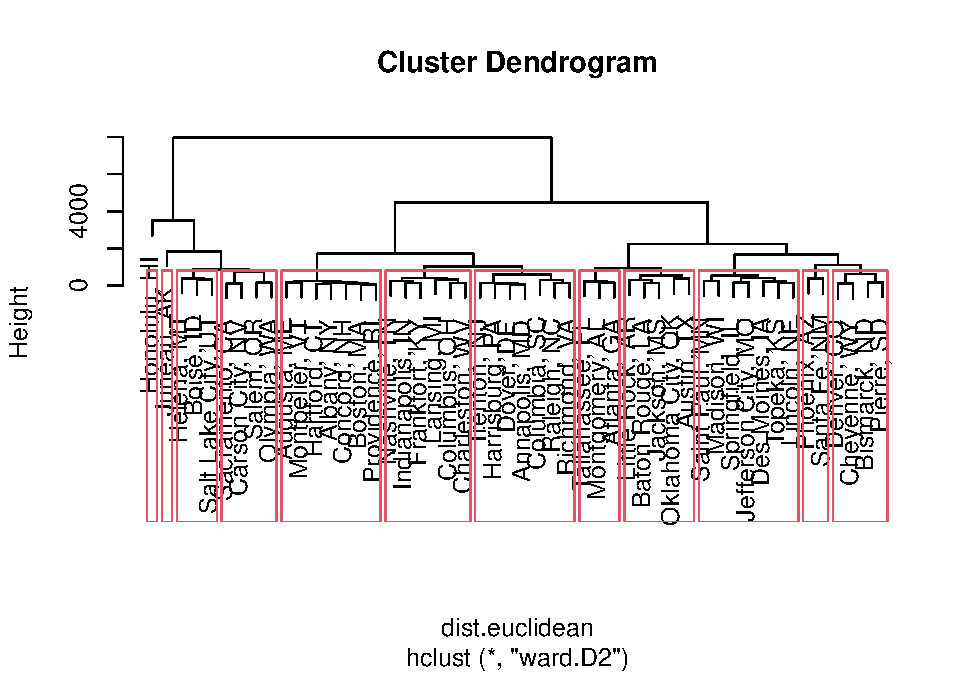
\includegraphics{graphics/chunk-distances-hclust-euclidean-1.pdf}

\begin{Shaded}
\begin{Highlighting}[]
\CommentTok{\#\# complete}
\CommentTok{\# }
\CommentTok{\# hclust.complete.dist.euclidean = hclust(dist.euclidean, method="complete");}
\CommentTok{\# }
\CommentTok{\# plot( hclust.ward2.dist.euclidean, }
\CommentTok{\#       labels= myLabels );}
\CommentTok{\# rect.hclust( hclust.ward2.dist.euclidean, k=12 );}
\CommentTok{\#   }
\end{Highlighting}
\end{Shaded}

\hypertarget{understanding-the-cutree}{%
\subsubsection{\texorpdfstring{Understanding the
\texttt{cutree}}{Understanding the cutree}}\label{understanding-the-cutree}}

In the above example, the tree was cut into 12 groups based on the
``distance'' formula used and based on the ``agglomeration'' linkage
technique invoice. I likely should have used a ``geo-spatial'' distance,
but we will see that mere ``euclidean'' distance seems to perform okay.

A fancy word for this statistical tree is a ``dendrogram''. I call each
element of the tree a branch. The smallest branches (twigs) are the
fundamental elements, in this case the cities. Over time, they merge
with other small branches, and so on.

The relative height when this smallest branch merges with another branch
demonstrates when the branch has found a similar pair-wise match (with
another smallest branch or a merging branch). I call ``Honolulu Hawaii''
an isolate because the vertical height when it merges with another
branch is the highest of all of the smallest branches (e.g., cities).
``Juneau Alaska'' is another isolate, but it does merge before
``Hawaii''.

It would be nice if we could decompose this information and look at one
\texttt{cutree} at a time. And color-code the distinctions. Using the
function \texttt{plot.hclust.sub} we can do this.

\begin{Shaded}
\begin{Highlighting}[]
\KeywordTok{source\_url}\NormalTok{( }\KeywordTok{paste0}\NormalTok{(path.github,}\StringTok{"humanVerseWSU/R/functions{-}EDA.R"}\NormalTok{) );  }\CommentTok{\# EDA functions ...}
\end{Highlighting}
\end{Shaded}

\begin{verbatim}
## SHA-1 hash of file is dd72e464241952b23d5b08d2213099eccf7a86f6
\end{verbatim}

\begin{Shaded}
\begin{Highlighting}[]
\NormalTok{hclust.ward2.dist.euclidean}\OperatorTok{$}\NormalTok{labels =}\StringTok{ }\NormalTok{myLabels;}
\KeywordTok{plot.hclust.sub}\NormalTok{(hclust.ward2.dist.euclidean, }\DataTypeTok{k=}\DecValTok{12}\NormalTok{);}
\end{Highlighting}
\end{Shaded}

\begin{verbatim}
## Registered S3 method overwritten by 'dendextend':
##   method       from   
##   text.pvclust pvclust
\end{verbatim}

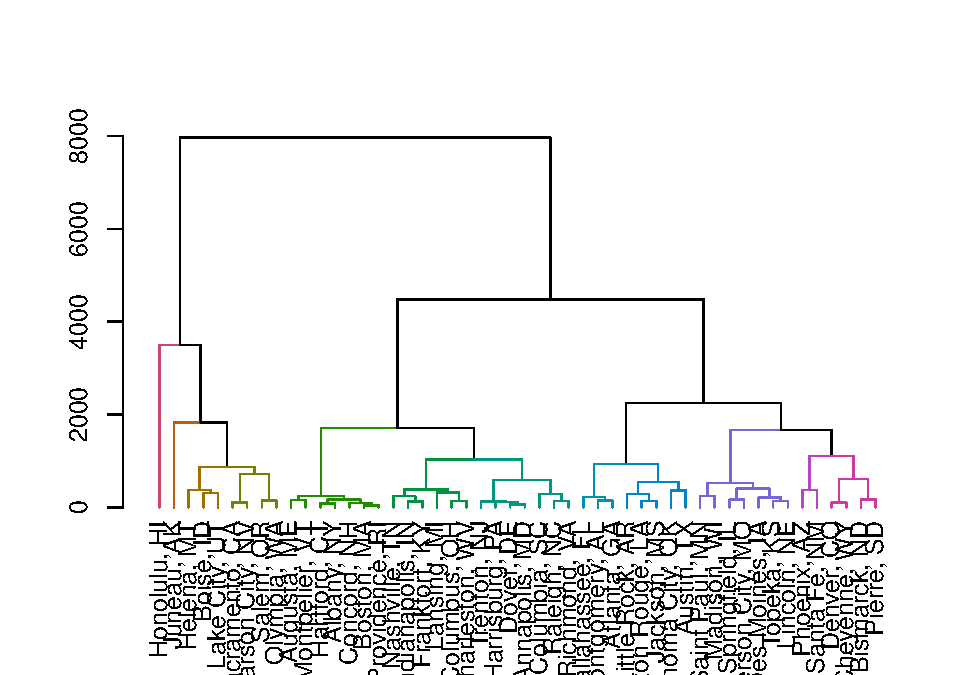
\includegraphics{graphics/chunk-distances-hclust-euclidean-sub-1.pdf}

\begin{verbatim}
## [1] "Pruning 1 of 12"
## [1] "Pruning 2 of 12"
## [1] "Pruning 3 of 12"
## [1] "Pruning 4 of 12"
## [1] "Pruning 5 of 12"
## [1] "Pruning 6 of 12"
## [1] "Pruning 7 of 12"
## [1] "Pruning 8 of 12"
## [1] "Pruning 9 of 12"
## [1] "Pruning 10 of 12"
## [1] "Pruning 11 of 12"
## [1] "Pruning 12 of 12"
\end{verbatim}

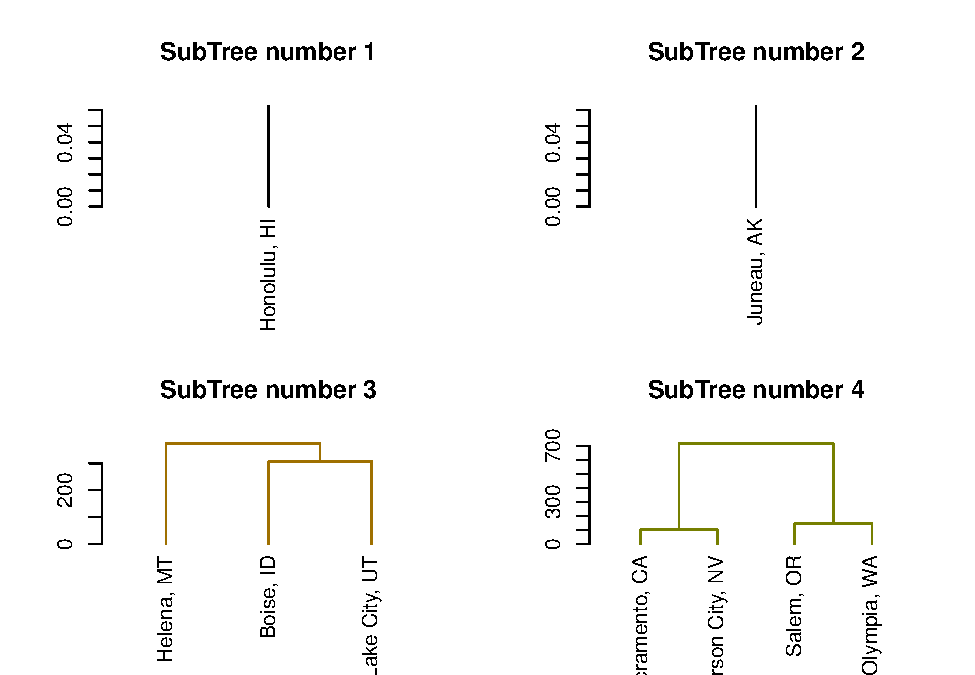
\includegraphics{graphics/chunk-distances-hclust-euclidean-sub-2.pdf}
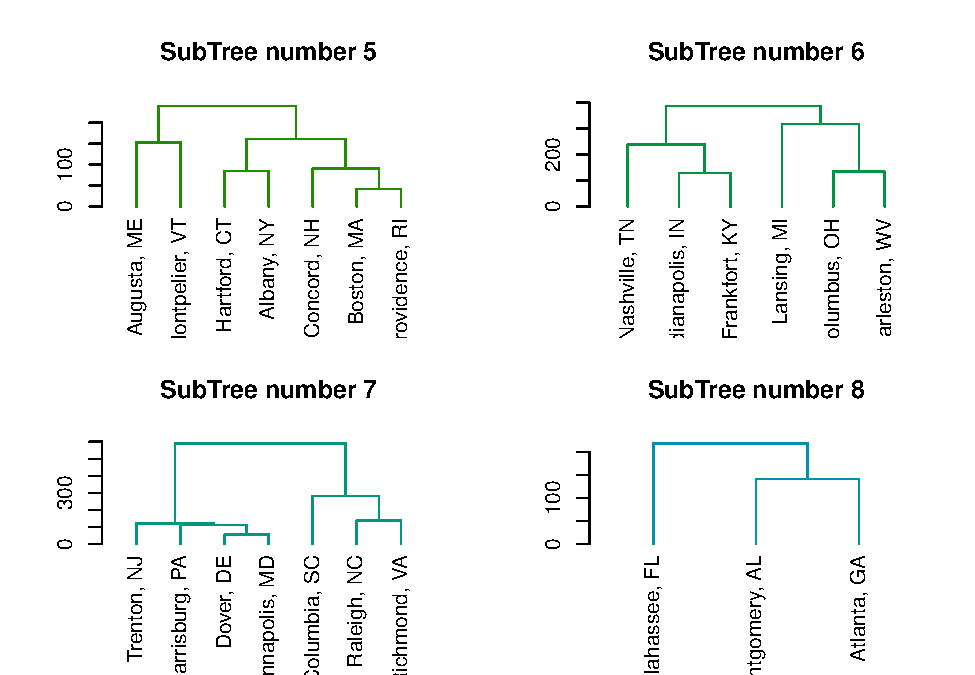
\includegraphics{graphics/chunk-distances-hclust-euclidean-sub-3.pdf}
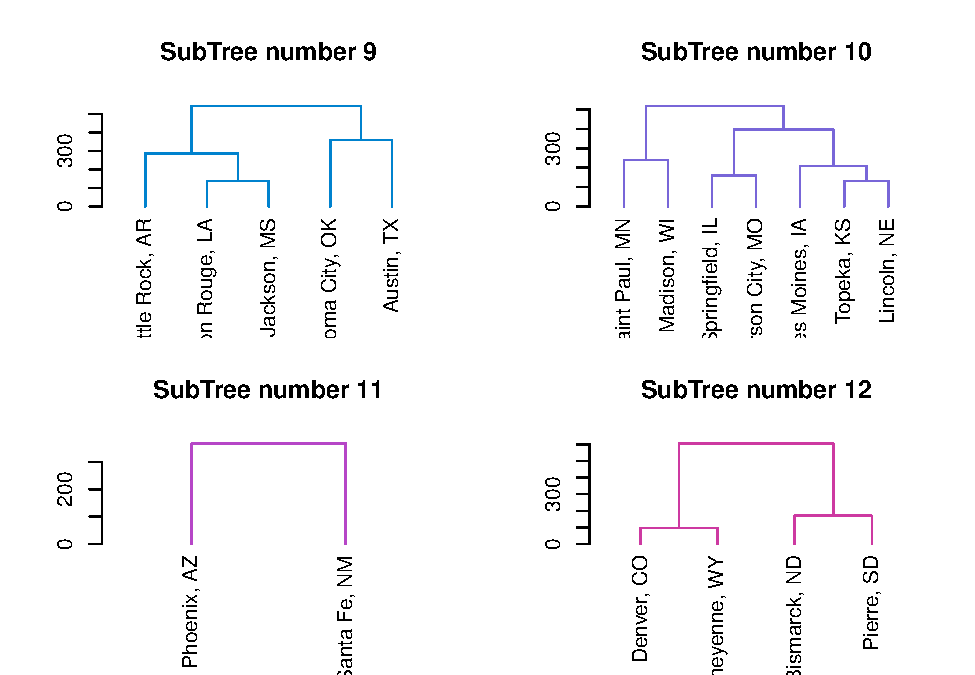
\includegraphics{graphics/chunk-distances-hclust-euclidean-sub-4.pdf}

\begin{Shaded}
\begin{Highlighting}[]
\CommentTok{\# plot.hclust.sub(hclust.complete.dist.euclidean, k=12);}
\end{Highlighting}
\end{Shaded}

\hypertarget{points-review-one-clustering-tree-dendrogram}{%
\subsubsection{(10 points) Review one clustering tree
(dendrogram)}\label{points-review-one-clustering-tree-dendrogram}}

Choose either \texttt{hclust.ward2.dist.euclidean} or
\texttt{hclust.complete.dist.euclidean} and review how the U.S. state
capitals are clustered. {[}I commented out one form, so you will have to
re-run if you want to select that one.{]}

Comment on the ``face validity'' of this approach based on your
understanding about how the U.S. regions are defined? Are the
North/South Dakotas together? What about the North/South Carolinas? What
about the Pacific Northwest? While living in Kentucky, some people
called the area ``Kentuckiana'' meaning Kentucky/Indiana. Does that show
up? Also note anything that seems peculiar.

\hypertarget{additional-remarks-about-hclust}{%
\subsubsection{\texorpdfstring{Additional remarks about
\texttt{hclust}}{Additional remarks about hclust}}\label{additional-remarks-about-hclust}}

I find \texttt{hclust} to be a nice initial perusal of the data.

If you want to understand the stability of a particular \texttt{hclust}
to use it for something other than an ``initial perusal of the data,'' I
would recommend \texttt{pvclust} which I introduced in the weekly
notebooks. It is often used in peer-reviewed research, as it provides a
\texttt{p-value} of sorts regarding the \textbf{stability} of the
\texttt{hclust} structure.

\hypertarget{generic-clustering}{%
\subsection{GENERIC clustering}\label{generic-clustering}}

Aggregating or agglomerating data is typically called ``clustering''. In
exploration, we can create some generic clustering techniques. Below we
will create two adhoc clustering rules.

\hypertarget{arbitrary-aggregation}{%
\subsubsection{Arbitrary Aggregation}\label{arbitrary-aggregation}}

Recall the ``movie dataset'' with ``Will Smith'' and ``Denzel
Washington''. We have a collection of movies, and how much money each
movie made at the box office. We could organize those movies by some
arbitrary rules. For example:

\begin{itemize}
\tightlist
\item
  Cluster 1: NA. We have missing data regarding the money. So let's put
  all movies that are NA into that cluster.
\item
  Cluster 2: Under a million dollars
\item
  Cluster 3: 1-4.99\ldots{} million dollars (greater than or equal to
  one, but less than 5)
\item
  Cluster 4: 5-49.99\ldots{}
\item
  Cluster 5: 50+
\end{itemize}

\hypertarget{points-movie-aggregation-arbitrary-for-will-and-denzel}{%
\paragraph{(5 points) Movie Aggregation {[}Arbitrary{]} for Will and
Denzel}\label{points-movie-aggregation-arbitrary-for-will-and-denzel}}

\begin{Shaded}
\begin{Highlighting}[]
\KeywordTok{library}\NormalTok{(devtools);}
\KeywordTok{source\_url}\NormalTok{( }\KeywordTok{paste0}\NormalTok{(path.mshaffer, }\StringTok{"will"}\NormalTok{) );}
\end{Highlighting}
\end{Shaded}

\begin{verbatim}
## SHA-1 hash of file is 3c1c97d961577e9b47a12faa20dca74bfe755c87
\end{verbatim}

\begin{Shaded}
\begin{Highlighting}[]
\KeywordTok{source\_url}\NormalTok{( }\KeywordTok{paste0}\NormalTok{(path.mshaffer, }\StringTok{"denzel"}\NormalTok{) );}
\end{Highlighting}
\end{Shaded}

\begin{verbatim}
## SHA-1 hash of file is 6692d8c5629db1ae023691bb55de2664a48cdde0
\end{verbatim}

\begin{Shaded}
\begin{Highlighting}[]
\NormalTok{movies}\FloatTok{.50}\NormalTok{ =}\StringTok{ }\KeywordTok{rbind}\NormalTok{(will}\OperatorTok{$}\NormalTok{movies}\FloatTok{.50}\NormalTok{, denzel}\OperatorTok{$}\NormalTok{movies}\FloatTok{.50}\NormalTok{);}

\KeywordTok{unique}\NormalTok{(movies}\FloatTok{.50}\OperatorTok{$}\NormalTok{ttid); }\CommentTok{\# are they in any shared movies ???}
\end{Highlighting}
\end{Shaded}

\begin{verbatim}
##   [1] "tt0480249" "tt1386697" "tt0116629" "tt0119654" "tt0343818" "tt0454921"
##   [7] "tt0448157" "tt0120912" "tt1409024" "tt0386588" "tt0814314" "tt0112442"
##  [13] "tt0172156" "tt0120660" "tt6139732" "tt0145660" "tt2381941" "tt1815862"
##  [19] "tt1596350" "tt1229340" "tt5519340" "tt0307453" "tt1155076" "tt0120891"
##  [25] "tt0120783" "tt1502397" "tt0248667" "tt4682786" "tt3322364" "tt1025100"
##  [31] "tt0114558" "tt0300051" "tt0284490" "tt0146984" "tt1837709" "tt0338466"
##  [37] "tt0947802" "tt1823664" "tt0268397" "tt1082886" "tt5814534" "tt3721964"
##  [43] "tt0416212" "tt0108149" "tt0328099" "tt0167427" "tt0466839" "tt0107478"
##  [49] "tt7255568" "tt0466856" "tt0765429" "tt0139654" "tt0454848" "tt0455944"
##  [55] "tt0328107" "tt1907668" "tt0453467" "tt1037705" "tt0107818" "tt1599348"
##  [61] "tt0210945" "tt1272878" "tt1111422" "tt0477080" "tt2404435" "tt0145681"
##  [67] "tt3766354" "tt0251160" "tt0097441" "tt0368008" "tt0112740" "tt2671706"
##  [73] "tt0174856" "tt0104797" "tt0107798" "tt0119099" "tt0133952" "tt0313443"
##  [79] "tt0427309" "tt0115956" "tt0107616" "tt0124718" "tt0168786" "tt6000478"
##  [85] "tt0114857" "tt0112857" "tt0102789" "tt0092804" "tt0100168" "tt0117372"
##  [91] "tt0088146" "tt0097880" "tt0102456" "tt0099750" "tt0091786" "tt0082138"
##  [97] "tt0097373" "tt4283892" "tt1698652" "tt0118783"
\end{verbatim}

\begin{Shaded}
\begin{Highlighting}[]
\KeywordTok{loadInflationData}\NormalTok{();}

\NormalTok{movies}\FloatTok{.50}\NormalTok{ =}\StringTok{ }\KeywordTok{standardizeDollarsInDataFrame}\NormalTok{(movies}\FloatTok{.50}\NormalTok{, }
                \DecValTok{2000}\NormalTok{, }
                \StringTok{"millions"}\NormalTok{, }
                \StringTok{"year"}\NormalTok{, }
                \StringTok{"millionsAdj2000"}\NormalTok{);}

\NormalTok{movies}\FloatTok{.50}\OperatorTok{$}\NormalTok{cluster.arbitrary =}\StringTok{ }\OtherTok{NA}\NormalTok{;}
\KeywordTok{str}\NormalTok{(movies}\FloatTok{.50}\NormalTok{);}
\end{Highlighting}
\end{Shaded}

\begin{verbatim}
## 'data.frame':    100 obs. of  13 variables:
##  $ rank             : num  1 2 3 4 5 6 7 8 9 10 ...
##  $ title            : chr  "I Am Legend" "Suicide Squad" "Independence Day" "Men in Black" ...
##  $ ttid             : chr  "tt0480249" "tt1386697" "tt0116629" "tt0119654" ...
##  $ year             : num  2007 2016 1996 1997 2004 ...
##  $ rated            : chr  "PG-13" "PG-13" "PG-13" "PG-13" ...
##  $ minutes          : num  101 123 145 98 115 117 92 88 106 118 ...
##  $ genre            : chr  "Action, Adventure, Drama" "Action, Adventure, Fantasy" "Action, Adventure, Sci-Fi" "Action, Adventure, Comedy" ...
##  $ ratings          : num  7.2 6 7 7.3 7.1 8 6.4 6.2 6.8 6.6 ...
##  $ metacritic       : num  65 40 59 71 59 64 49 49 58 58 ...
##  $ votes            : num  675193 588111 520657 507618 491489 ...
##  $ millions         : num  256 325 306 251 145 ...
##  $ millionsAdj2000  : num  213 233 336 269 132 ...
##  $ cluster.arbitrary: logi  NA NA NA NA NA NA ...
\end{verbatim}

\begin{Shaded}
\begin{Highlighting}[]
\CommentTok{\#\# you do something here ... }

\CommentTok{\# (1) populate cluster.arbitrary}
\CommentTok{\# (2) summarize how many movies live in each (table count)}
\end{Highlighting}
\end{Shaded}

\hypertarget{aggregating-using-quantiles}{%
\subsubsection{Aggregating using
Quantiles}\label{aggregating-using-quantiles}}

John Tukey emphasized that ordering the data and then splitting it based
on the ordering was a fundamental premise of exploratory data analysis.

\hypertarget{tukeys-summary-data}{%
\paragraph{Tukey's Summary Data}\label{tukeys-summary-data}}

John Tukey proposed five elements as primary data for analysis.

\begin{itemize}
\tightlist
\item
  the minimum \texttt{min}
\item
  the maximum \texttt{max}
\end{itemize}

Sorting the data makes it easiest to find these data, and will be useful
to find the other three exploratory summary features.

This is what I would call ``slice and dice''. The data is cut in half,
and the value of that middle ``cutting point'' is the \texttt{Q2} which
we call the \texttt{median}.

Next, the lower half could also be cut in half, and the value of that
middle ``cutting'' point is \texttt{Q1}.

Then, the upper half could also be cut in half, and the value of that
middle ``cutting'' point is \texttt{Q3}.

A common metric derived from this ``median-split'' procedure is called
the interquartile range \texttt{IQR} which is defined as the distance
between \texttt{Q3} and \texttt{Q1}. It literally represents the middle
50\% of the data; 50\% of the elements of the dataset are between
\texttt{Q3} and \texttt{Q1}.

\hypertarget{quartile-example}{%
\paragraph{Quartile Example}\label{quartile-example}}

\begin{Shaded}
\begin{Highlighting}[]
\NormalTok{x =}\StringTok{ }\DecValTok{1}\OperatorTok{:}\DecValTok{99}\NormalTok{;}
\KeywordTok{length}\NormalTok{(x);}
\end{Highlighting}
\end{Shaded}

\begin{verbatim}
## [1] 99
\end{verbatim}

\begin{Shaded}
\begin{Highlighting}[]
\KeywordTok{median}\NormalTok{(x);}
\end{Highlighting}
\end{Shaded}

\begin{verbatim}
## [1] 50
\end{verbatim}

\begin{Shaded}
\begin{Highlighting}[]
\NormalTok{x[}\DecValTok{50}\NormalTok{];}
\end{Highlighting}
\end{Shaded}

\begin{verbatim}
## [1] 50
\end{verbatim}

\begin{Shaded}
\begin{Highlighting}[]
\KeywordTok{median}\NormalTok{(x[}\DecValTok{1}\OperatorTok{:}\DecValTok{49}\NormalTok{]);}
\end{Highlighting}
\end{Shaded}

\begin{verbatim}
## [1] 25
\end{verbatim}

\begin{Shaded}
\begin{Highlighting}[]
\NormalTok{x[}\DecValTok{25}\NormalTok{];}
\end{Highlighting}
\end{Shaded}

\begin{verbatim}
## [1] 25
\end{verbatim}

\begin{Shaded}
\begin{Highlighting}[]
\KeywordTok{median}\NormalTok{(x[}\DecValTok{51}\OperatorTok{:}\DecValTok{99}\NormalTok{]);}
\end{Highlighting}
\end{Shaded}

\begin{verbatim}
## [1] 75
\end{verbatim}

\begin{Shaded}
\begin{Highlighting}[]
\NormalTok{x[}\DecValTok{75}\NormalTok{];}
\end{Highlighting}
\end{Shaded}

\begin{verbatim}
## [1] 75
\end{verbatim}

\begin{Shaded}
\begin{Highlighting}[]
\CommentTok{\# probability{-}approach ... }
\CommentTok{\# algorithm: the default type=7}
\NormalTok{stats}\OperatorTok{::}\KeywordTok{quantile}\NormalTok{(x, }\DataTypeTok{prob =} \KeywordTok{c}\NormalTok{(}\FloatTok{0.25}\NormalTok{, }\FloatTok{0.5}\NormalTok{, }\FloatTok{0.75}\NormalTok{), }\DataTypeTok{type=}\DecValTok{1}\NormalTok{);}
\end{Highlighting}
\end{Shaded}

\begin{verbatim}
## 25% 50% 75% 
##  25  50  75
\end{verbatim}

Algorithms address various issues associated with dividing numbers and
whether or not to include the dividing number in the subset division,
but the principle holds.

We can generalize this idea by not always cutting the data in half
(median-split as \texttt{n=2}, median-median-split as \texttt{n=4}).
Instead, we could cut by tens (we call them deciles). Or we could cut by
hundreds (we call them centiles). The function \texttt{quantile}
performs this operation, and if you dig into the \texttt{doStatsSummary}
function used in this course, you can see its application.

\hypertarget{points-movie-aggregation-decile-for-will-and-denzel}{%
\paragraph{(5 points) Movie Aggregation {[}Decile{]} for Will and
Denzel}\label{points-movie-aggregation-decile-for-will-and-denzel}}

\begin{Shaded}
\begin{Highlighting}[]
\NormalTok{movies}\FloatTok{.50}\OperatorTok{$}\NormalTok{cluster.deciles =}\StringTok{ }\OtherTok{NA}\NormalTok{;}
\KeywordTok{str}\NormalTok{(movies}\FloatTok{.50}\NormalTok{);}
\end{Highlighting}
\end{Shaded}

\begin{verbatim}
## 'data.frame':    100 obs. of  14 variables:
##  $ rank             : num  1 2 3 4 5 6 7 8 9 10 ...
##  $ title            : chr  "I Am Legend" "Suicide Squad" "Independence Day" "Men in Black" ...
##  $ ttid             : chr  "tt0480249" "tt1386697" "tt0116629" "tt0119654" ...
##  $ year             : num  2007 2016 1996 1997 2004 ...
##  $ rated            : chr  "PG-13" "PG-13" "PG-13" "PG-13" ...
##  $ minutes          : num  101 123 145 98 115 117 92 88 106 118 ...
##  $ genre            : chr  "Action, Adventure, Drama" "Action, Adventure, Fantasy" "Action, Adventure, Sci-Fi" "Action, Adventure, Comedy" ...
##  $ ratings          : num  7.2 6 7 7.3 7.1 8 6.4 6.2 6.8 6.6 ...
##  $ metacritic       : num  65 40 59 71 59 64 49 49 58 58 ...
##  $ votes            : num  675193 588111 520657 507618 491489 ...
##  $ millions         : num  256 325 306 251 145 ...
##  $ millionsAdj2000  : num  213 233 336 269 132 ...
##  $ cluster.arbitrary: logi  NA NA NA NA NA NA ...
##  $ cluster.deciles  : logi  NA NA NA NA NA NA ...
\end{verbatim}

\begin{Shaded}
\begin{Highlighting}[]
\CommentTok{\#\# you do something here ... }

\CommentTok{\# use \# stats::quantile(x, prob=seq(0.1,0.9,by=0.1), type=1 );}
\CommentTok{\# (1) how many NA\textquotesingle{}s are there ... keep them NA\textquotesingle{}s}
\CommentTok{\# (2) for the rest of the data, break it up into deciles}
\CommentTok{\# (3) $cluster.deciles for a given movie should be NA, 1, 2, 3, ... 10}
\CommentTok{\# (4) summarize how many movies live in each (table count)}
\end{Highlighting}
\end{Shaded}

\hypertarget{centroid-clustering-k-means-as-a-function-of-distance}{%
\subsection{CENTROID clustering (k-means) as a function of
distance}\label{centroid-clustering-k-means-as-a-function-of-distance}}

\hypertarget{introduction-2}{%
\subsubsection{Introduction}\label{introduction-2}}

Rather than clustering on distance-linkage in a pair-wise fashion, we
can cluster based on randomly selecting just \texttt{k} points in our
data and begin identifying their nearest neighbors using some distance
approach.

For example, if \texttt{k=3}, we would randomly select three of our data
points. We would then compute the distances from all of the remaining
points to these \texttt{3} anchor points. The points that are closest to
a given anchor will be assigned to that anchor. At the end of the stage,
we now have new data, so a new centroid is determined. At this point,
the centroid \url{https://en.wikipedia.org/wiki/Centroid} is likely not
one of our data points, but a location within the given centroid
cluster. In the ``naive'' approach, you merely take an average (mean) of
all the members of your cluster. More advanced approaches (the default
``Hartigan-Wong'' of \texttt{kmeans}) utilize deviations from the
average, called a sum-of-squares approach. This is why in our
\texttt{kmeans-notebook} we analyzed the \texttt{wss} to ascertain how
many clusters \texttt{k} should we use.

Regardless, after the new centroids (centers) for the clusters are
determined, the process iterates. All distances are computed from all
points to the new centroids; points are assigned to a given centroid
cluster (in this example: 1, 2, 3); a new centroid center is computed,
and we repeat the process until a stopping rule is reached: maybe we
have exhausted the number of iterations allowed (\texttt{iter.max}
parameter of \texttt{kmeans})? Or maybe we are not changing membership
of any of the data points? Or maybe we have met some objective (like
\texttt{wss})?

It is possible to get a \texttt{kmeans} result by merely starting with
\texttt{3\ different} random points. In general, \texttt{kmeans} is fast
(and our computers are so much faster than the computers of 1990: the
first computer I built in 1995 had 32MB of RAM, a Pentium processor
\url{https://en.wikipedia.org/wiki/Pentium\#Pentium} and a 900MB Cheetah
hard-drive).

Anyway, we can utilize the parameter \texttt{nstart} to try many
different starting values, and let the program identify the best, most
consistent solution.

\hypertarget{my-recommendations}{%
\subsubsection{My recommendations}\label{my-recommendations}}

I would recommend the default algorithm \texttt{Hartigan-Wong} with
\texttt{iter.max=100} and \texttt{nstart=100}. You can test the timings
from the default values: \texttt{iter.max=10} and \texttt{nstart=1}.
Since the data is likely multidimensional \texttt{stars} are the best
way to summary the results and membership of \texttt{kmeans}. Please see
the ``kmeans-notebook'' for examples.

\hypertarget{wikipedia-climate-data}{%
\subsubsection{WIKIPEDIA CLIMATE DATA}\label{wikipedia-climate-data}}

For the 50 U.S. cities, we harvested climate data. In the ``Wikipedia''
notebook, details of that data provenance were outlined. If we want to
compare the cities using the climate data, we have to build a matching
dataframe, which means we have to select features that exist in each
city's climate data set.

There are four temperature features that are always present:

\begin{itemize}
\tightlist
\item
  Record high F (C) \ldots{} we will call it ``high.max''
\item
  Average high F (C) \ldots{} we will call it ``high.avg''
\item
  Average low F (C) \ldots{} we will call it ``low.avg''
\item
  Record low F (C) \ldots{} we will call it ``low.max'' {[}probably not
  the best name choice, but it is parallel in form to the first
  element{]}
\end{itemize}

Additionally, for precipitation we have:

\begin{itemize}
\tightlist
\item
  Average precipitation inches (mm) \ldots{} we will call it ``rain''
\item
  Average snowfall inches (cm) \ldots{} we will call it ``snow''
\end{itemize}

For each of these features we have 12 months of data. This is a nice
dataset. Let's see what we can do with it.

\hypertarget{basic-background-research}{%
\paragraph{Basic Background Research}\label{basic-background-research}}

We should begin by doing a bit of peripheral research on the topic, to
gain ``domain knowledge'' so we know what to do with the data. A few
elements that would benefit.

\url{https://www.forbes.com/sites/brianbrettschneider/2018/07/08/when-does-the-hottest-day-of-the-year-usually-occur/\#78141f47548c}

\textbf{Source: \url{https://bit.ly/359HAnY}}

\url{https://www.climate.gov/news-features/featured-images/whats-coldest-day-year}

\hypertarget{one-graph}{%
\paragraph{One Graph}\label{one-graph}}

When graphing data to visualize, it is essential that you keep the
scales uniform so quick-visual comparisons are accurate. I gave you a
task to practice the idea of creation that ``one informative'' research
graphic. And I now present my version for you to use and critique based
on your efforts. I am a \texttt{plot} guy, so some of you may have a
different `\texttt{ggplot2} type solution. Ultimately, the intent of
this graphic is to best summarize the data in a meaninful way for
exploratory analysis.

\hypertarget{points-one-research-graph}{%
\subparagraph{(5 points) One Research
Graph}\label{points-one-research-graph}}

\begin{Shaded}
\begin{Highlighting}[]
\NormalTok{climate =}\StringTok{ }\NormalTok{utils}\OperatorTok{::}\KeywordTok{read.csv}\NormalTok{( }\KeywordTok{paste0}\NormalTok{(path.mshaffer, }\StringTok{"\_data\_/state{-}capitals/final/state{-}capitals{-}climatedata.txt"}\NormalTok{), }\DataTypeTok{header=}\OtherTok{TRUE}\NormalTok{, }\DataTypeTok{quote=}\StringTok{""}\NormalTok{, }\DataTypeTok{sep=}\StringTok{"|"}\NormalTok{);}


\KeywordTok{plotTemperatureFromWikipediaData}\NormalTok{(climate, }\DataTypeTok{city.key=}\StringTok{"capital"}\NormalTok{, }\DataTypeTok{city.val=}\StringTok{"Helena"}\NormalTok{);}
\end{Highlighting}
\end{Shaded}

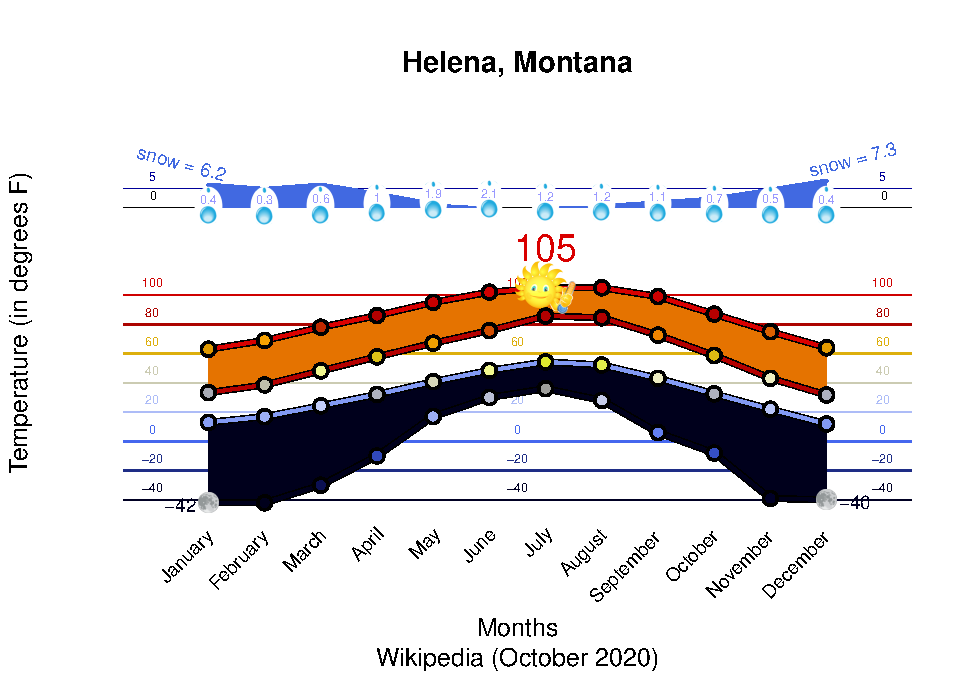
\includegraphics{graphics/chunk-hclust-climate-one-research-graph-1.pdf}

\begin{Shaded}
\begin{Highlighting}[]
\KeywordTok{plotTemperatureFromWikipediaData}\NormalTok{(climate, }\DataTypeTok{city.key=}\StringTok{"capital"}\NormalTok{, }\DataTypeTok{city.val=}\StringTok{"Baton Rouge"}\NormalTok{);}
\end{Highlighting}
\end{Shaded}

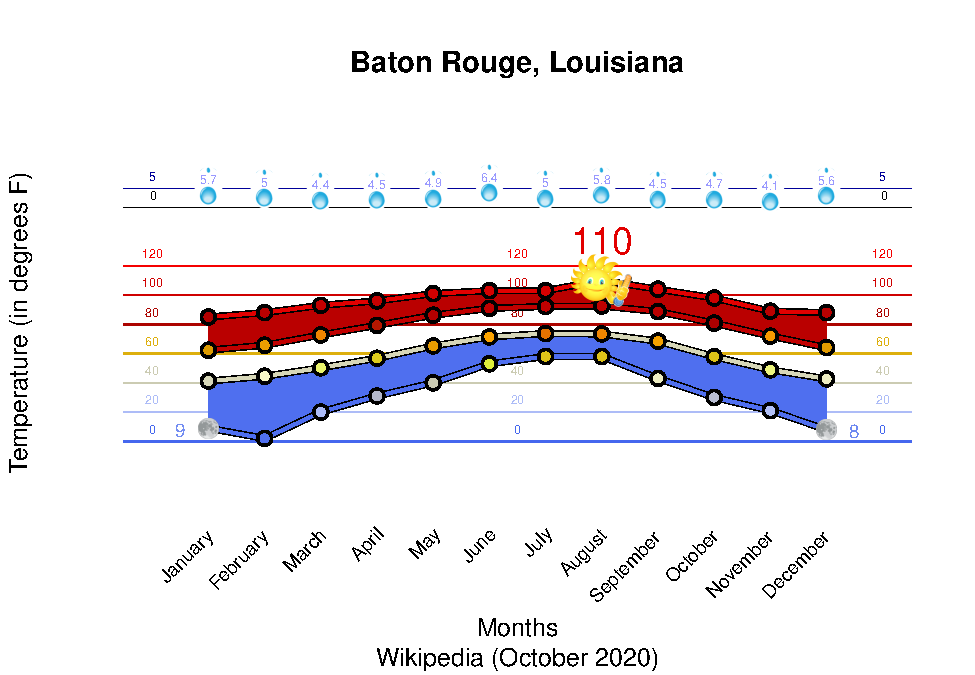
\includegraphics{graphics/chunk-hclust-climate-one-research-graph-2.pdf}

{[} What do you like about this graphic?

What do you dislike?

Is it aesthetically pleasing? Is it functional?

{]}

We can achieve a side-by-side comparison using the function described
below. The first city will be graphed on the left, the second city on
the right.

\begin{Shaded}
\begin{Highlighting}[]
\KeywordTok{compareTwoCitiesClimates}\NormalTok{(climate, }\DataTypeTok{city.key=}\StringTok{"capital"}\NormalTok{, }\DataTypeTok{city.1=}\StringTok{"Helena"}\NormalTok{, }\DataTypeTok{city.2=}\StringTok{"Baton Rouge"}\NormalTok{);}
\end{Highlighting}
\end{Shaded}

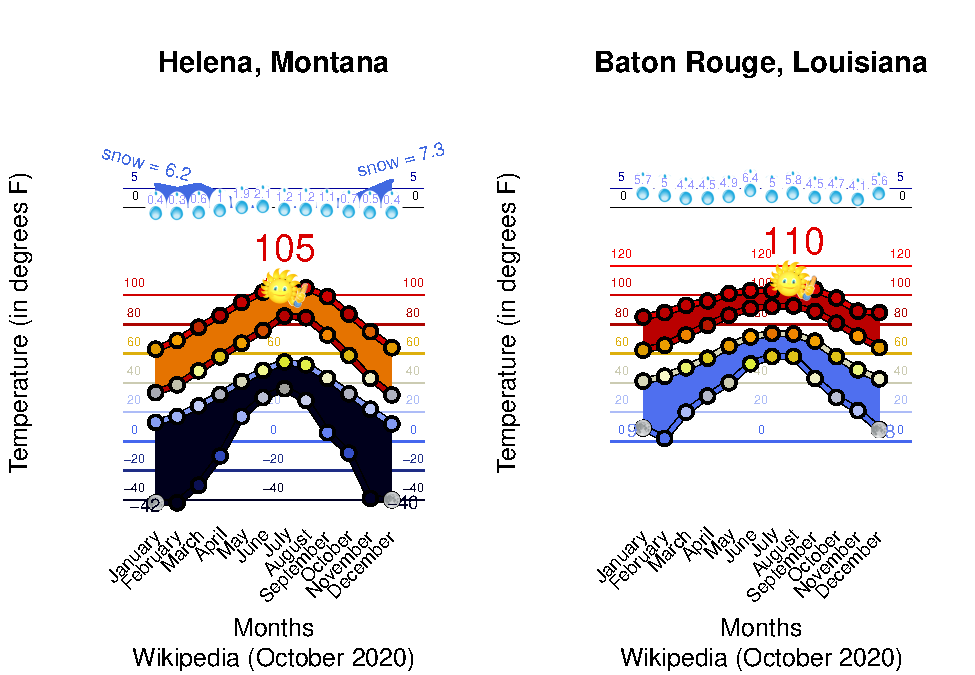
\includegraphics{graphics/chunk-hclust-climate-one-research-graph-comparison-1.pdf}

{[} What do you like about this graphic?

What do you dislike?

Are the y-axis the same scale? Are the visible gridlines for each the
same?

What is the difference between rain and snow on the graphic? Was that a
good approach? How would you have done it?

{]}

\hypertarget{points-one-publication-graph}{%
\subparagraph{(5 points) One Publication
Graph}\label{points-one-publication-graph}}

We are in exploration, so the ``one'' research graphic may be very
different than the ``one'' formal graphic designed for a client.
Typically, the final graphic needs to meet certain criteria:

\begin{itemize}
\tightlist
\item
  Very pleasing aesthetically
\item
  Interactive if possible
\item
  Live data feeds if possible
\item
  Served in a secure, safe, private location (if required by the client)
\end{itemize}

To demonstrate the differences, I created a mockup of our 50 U.S. cities
and put it into a nice finalized product form called ``highcharts''.

\url{http://md5.mshaffer.com/WSU_STATS419/_EXAMPLES_/fiddle_usmap/}

It pulls data in real time (using AJAX) to grab the weather at the
latitudes/longitudes we defined in our Wikipedia notebook.

\begin{itemize}
\tightlist
\item
  You can use your mouse to draw a box to zoom in.\\
\item
  The third-wheel on the mouse also helps you zoom in/out.
\item
  Hold down CNTRL with your left hand and use your mouse key to drag the
  map. It seems to only ``pan'' in the x-direction at the moment.\\
\item
  The data in the popup displayed can be customized. I report the
  temperature in Celsius/Fahrenheit and also display the population data
  we gathered from Wikipedia.
\end{itemize}

Once you have a template built, it is rather easy to modify it. Here I
changed the background map, and all of the data/features stay the same:

\url{http://md5.mshaffer.com/WSU_STATS419/_EXAMPLES_/fiddle_usmap/world.html}

\hypertarget{which-features-to-include-in-the-analysis}{%
\subsubsection{Which Features to Include in the
Analysis}\label{which-features-to-include-in-the-analysis}}

\begin{itemize}
\tightlist
\item
  months, you can pick all of them \texttt{1:12} or maybe just one month
  per season (April, July, October, January)
\item
  X, depending on what you chose for months, you can now select what
  climate columns you want to use

  \begin{itemize}
  \tightlist
  \item
    Some of Temperature Data
  \item
    All of Temperature Data
  \item
    Precipitation Data
  \item
    Everything (All of Temperature Data, Precipitation Data)
  \end{itemize}
\end{itemize}

If we want to cluster cities, which decisions seem best? Why? As you can
see from the code below, you just comment out two options, and can
quickly rerun the analysis.

\begin{itemize}
\tightlist
\item
  WHICH MONTHS
\item
  WHICH COLUMNS
\end{itemize}

\hypertarget{which-months-which-columns}{%
\paragraph{WHICH MONTHS \& WHICH
COLUMNS}\label{which-months-which-columns}}

\begin{Shaded}
\begin{Highlighting}[]
\NormalTok{climate =}\StringTok{ }\NormalTok{utils}\OperatorTok{::}\KeywordTok{read.csv}\NormalTok{( }\KeywordTok{paste0}\NormalTok{(path.mshaffer, }\StringTok{"\_data\_/state{-}capitals/final/state{-}capitals{-}climatedata.txt"}\NormalTok{), }\DataTypeTok{header=}\OtherTok{TRUE}\NormalTok{, }\DataTypeTok{quote=}\StringTok{""}\NormalTok{, }\DataTypeTok{sep=}\StringTok{"|"}\NormalTok{);}

\CommentTok{\#\#\#\#\#\#\#\#\#\#\#\#\#\#\#\#\#\#\#\#\# WHICH MONTHS \#\#\#\#\#\#\#\#\#\#\#\#\#\#\#\#\#\#\#\#\#}
\CommentTok{\#\#\#\#\#\#\#\#\#\#\#\#\#\#\#\#\#\#\#\#\#\#\#\#\#\#\#\#\#\#\#\#\#\#\#\#\#\#\#\#\#\#\#\#\#\#\#\#\#\#\#\#\#\#\#\#}
\NormalTok{months =}\StringTok{ }\DecValTok{1}\OperatorTok{:}\DecValTok{12}\NormalTok{; }\CommentTok{\# all the data}
\CommentTok{\#months = c(1,4,7,10); \# one month of each of the four seasons}
\CommentTok{\#\#\#\#\#\#\#\#\#\#\#\#\#\#\#\#\#\#\#\#\#\#\#\#\#\#\#\#\#\#\#\#\#\#\#\#\#\#\#\#\#\#\#\#\#\#\#\#\#\#\#\#\#\#\#\#}


\NormalTok{month.abb;  }\CommentTok{\# ?month.abb}
\end{Highlighting}
\end{Shaded}

\begin{verbatim}
##  [1] "Jan" "Feb" "Mar" "Apr" "May" "Jun" "Jul" "Aug" "Sep" "Oct" "Nov" "Dec"
\end{verbatim}

\begin{Shaded}
\begin{Highlighting}[]
\NormalTok{month.name;  }
\end{Highlighting}
\end{Shaded}

\begin{verbatim}
##  [1] "January"   "February"  "March"     "April"     "May"       "June"     
##  [7] "July"      "August"    "September" "October"   "November"  "December"
\end{verbatim}

\begin{Shaded}
\begin{Highlighting}[]
\NormalTok{month.name[months];  }\CommentTok{\# these are the names of the months you are selecting ...}
\end{Highlighting}
\end{Shaded}

\begin{verbatim}
##  [1] "January"   "February"  "March"     "April"     "May"       "June"     
##  [7] "July"      "August"    "September" "October"   "November"  "December"
\end{verbatim}

\begin{Shaded}
\begin{Highlighting}[]
\CommentTok{\# this function would allow us to use different months as criteria and different climate{-}data keys.  It is variadic and flexible.  \textasciigrave{}key.n\textasciigrave{} are the names we will use for our new columns ...}

\NormalTok{climate.df =}\StringTok{ }\KeywordTok{buildClimateDataFrame}\NormalTok{(climate, months, }\DataTypeTok{keys=}\KeywordTok{c}\NormalTok{(}\StringTok{"Record high F (C)"}\NormalTok{, }\StringTok{"Average high F (C)"}\NormalTok{, }\StringTok{"Average low F (C)"}\NormalTok{, }\StringTok{"Record low F (C)"}\NormalTok{, }\StringTok{"Average precipitation inches (mm)"}\NormalTok{, }\StringTok{"Average snowfall inches (cm)"}\NormalTok{), }\DataTypeTok{keys.n =} \KeywordTok{c}\NormalTok{(}\StringTok{"highmax"}\NormalTok{, }\StringTok{"highavg"}\NormalTok{,  }\StringTok{"lowavg"}\NormalTok{, }\StringTok{"lowmin"}\NormalTok{, }\StringTok{"rain"}\NormalTok{, }\StringTok{"snow"}\NormalTok{) );}

\NormalTok{climate.df;}
\end{Highlighting}
\end{Shaded}

\begin{verbatim}
##               state        capital st             labels highmax.Jan
## 1           Alabama     Montgomery AL     Montgomery, AL          83
## 23           Alaska         Juneau AK         Juneau, AK          60
## 39          Arizona        Phoenix AZ        Phoenix, AZ          88
## 59         Arkansas    Little Rock AR    Little Rock, AR          83
## 79       California     Sacramento CA     Sacramento, CA          79
## 94         Colorado         Denver CO         Denver, CO          76
## 117     Connecticut       Hartford CT       Hartford, CT          72
## 141        Delaware          Dover DE          Dover, DE          77
## 162         Florida    Tallahassee FL    Tallahassee, FL          83
## 182         Georgia        Atlanta GA        Atlanta, GA          79
## 205          Hawaii       Honolulu HI       Honolulu, HI          88
## 225           Idaho          Boise ID          Boise, ID          63
## 248        Illinois    Springfield IL    Springfield, IL          73
## 265         Indiana   Indianapolis IN   Indianapolis, IN          71
## 289            Iowa     Des Moines IA     Des Moines, IA          67
## 311          Kansas         Topeka KS         Topeka, KS          78
## 334        Kentucky      Frankfort KY      Frankfort, KY          80
## 350       Louisiana    Baton Rouge LA    Baton Rouge, LA          85
## 365           Maine        Augusta ME        Augusta, ME          61
## 381        Maryland      Annapolis MD      Annapolis, MD          77
## 399   Massachusetts         Boston MA         Boston, MA          74
## 423        Michigan        Lansing MI        Lansing, MI          66
## 446       Minnesota     Saint Paul MN     Saint Paul, MN          57
## 458     Mississippi        Jackson MS        Jackson, MS          85
## 476        Missouri Jefferson City MO Jefferson City, MO          79
## 490         Montana         Helena MT         Helena, MT          63
## 509        Nebraska        Lincoln NE        Lincoln, NE          73
## 532          Nevada    Carson City NV    Carson City, NV          72
## 552   New Hampshire        Concord NH        Concord, NH          72
## 574      New Jersey        Trenton NJ        Trenton, NJ          73
## 597      New Mexico       Santa Fe NM       Santa Fe, NM          65
## 617        New York         Albany NY         Albany, NY          71
## 641  North Carolina        Raleigh NC        Raleigh, NC          80
## 665    North Dakota       Bismarck ND       Bismarck, ND          63
## 688            Ohio       Columbus OH       Columbus, OH          74
## 712        Oklahoma  Oklahoma City OK  Oklahoma City, OK          83
## 734          Oregon          Salem OR          Salem, OR          68
## 754    Pennsylvania     Harrisburg PA     Harrisburg, PA          73
## 776    Rhode Island     Providence RI     Providence, RI          70
## 800  South Carolina       Columbia SC       Columbia, SC          84
## 823    South Dakota         Pierre SD         Pierre, SD          68
## 837       Tennessee      Nashville TN      Nashville, TN          78
## 861           Texas         Austin TX         Austin, TX          90
## 885            Utah Salt Lake City UT Salt Lake City, UT          63
## 908         Vermont     Montpelier VT     Montpelier, VT          66
## 925        Virginia       Richmond VA       Richmond, VA          81
## 949      Washington        Olympia WA        Olympia, WA          64
## 968   West Virginia     Charleston WV     Charleston, WV          81
## 986       Wisconsin        Madison WI        Madison, WI          58
## 1007        Wyoming       Cheyenne WY       Cheyenne, WY          70
##      highmax.Feb highmax.Mar highmax.Apr highmax.May highmax.Jun highmax.Jul
## 1             86          90          94          99         106         107
## 23            57          61          72          80          87          89
## 39            92         100         105         114         122         121
## 59            87          91          95          98         107         112
## 79            80          90          98         107         112         114
## 94            80          84          90          95         105         105
## 117           77          89          96          99         100         103
## 141           80          88          97          98         101         104
## 162           89          91          95         102         105         104
## 182           80          89          93          97         106         105
## 205           88          89          91          93          92          94
## 225           71          82          92         100         110         111
## 248           78          91          90         101         104         112
## 265           77          85          90          96         104         106
## 289           78          91          93         105         103         110
## 311           84          93          97         103         109         114
## 334           80          88          95          99         106         111
## 350           88          93          96         101         103         103
## 365           60          84          90          94          98          99
## 381           83          92          95          98         103         105
## 399           73          89          94          97         100         104
## 423           69          86          88          96          99         103
## 446           59          83          93          93         103         105
## 458           89          95          94         100         105         107
## 476           89          97          96         102         105         112
## 490           69          78          86          95         102         105
## 509           83          91          97         104         108         115
## 532           76          81          88          94         101         107
## 552           74          89          95          98         101         102
## 574           76          87          93          99         100         106
## 597           73          77          84          96          99         101
## 617           74          89          93          97         100         104
## 641           84          94          95          99         105         105
## 665           73          81          93         102         111         114
## 688           78          85          90          96         102         106
## 712           92          97         100         104         107         110
## 734           72          80          93         100         105         108
## 754           79          87          93          97         100         107
## 776           72          90          98          96          98         102
## 800           84          93          96         101         109         107
## 823           75          88          98         105         112         117
## 837           84          89          91          96         109         107
## 861           99          98          99         104         109         109
## 885           69          80          89          99         105         107
## 908           61          82          90          90          95          97
## 925           83          94          96         100         104         105
## 949           73          79          88          96          98         104
## 968           81          92          96          98         105         108
## 986           68          83          94         101         101         107
## 1007          71          77          84          91         100         100
##      highmax.Aug highmax.Sep highmax.Oct highmax.Nov highmax.Dec highavg.Jan
## 1            106         106         102          91          85        57.4
## 23            87          85          68          64          59        34.6
## 39           117         116         107          96          87        67.2
## 59           114         106          98          86          81        50.5
## 79           112         109         102          86          72        54.4
## 94           105         101          90          81          79        44.0
## 117          102         101          91          83          76        34.5
## 141          102          99          95          85          75        43.4
## 162          103         102          95          89          84        63.5
## 182          104         102          98          84          79        52.3
## 205           95          95          94          93          89        80.1
## 225          110         102          94          78          70        37.8
## 248          108         102          93          83          74        34.8
## 265          103         100          92          81          74        35.6
## 289          110         101          95          82          69        31.0
## 311          113         110          97          85          77        39.9
## 334          105         106          98          84          78        41.5
## 350          110         104          98          89          88        62.3
## 365          100          96          85          74          67        27.6
## 381          106          99          92          85          78        42.7
## 399          102         102          90          83          76        35.8
## 423          102          99          90          79          70        30.1
## 446          103          95          88          75          66        26.0
## 458          107         107          98          89          84        56.1
## 476          111         107          96          87          79        39.9
## 490          105          99          87          75          64        33.3
## 509          110         106          98          85          75        35.4
## 532          105         103          93          79          75        45.2
## 552          101          98          92          80          73        30.8
## 574          105         101          94          83          76        39.0
## 597           96          94          87          75          65        43.5
## 617          102         100          91          82          72        30.6
## 641          105         104         100          88          81        50.9
## 665          109         105          95          79          66        23.4
## 688          103         100          94          80          76        36.5
## 712          113         108          97          87          86        49.7
## 734          108         104          93          74          72        47.7
## 754          104         102          97          84          75        37.0
## 776          104         100          88          81          77        37.4
## 800          107         106         101          90          83        56.0
## 823          114         108          98          87          77        30.0
## 837          106         105          99          88          79        46.9
## 861          112         112         100          91          90        61.5
## 885          106         100          89          75          69        37.4
## 908           97          92          84          76          67        26.4
## 925          107         103          99          86          81        47.4
## 949          104          98          90          74          64        45.9
## 968          108         104          96          87          80        42.5
## 986          102          99          90          77          65        26.4
## 1007          98          95          85          75          69        39.5
##      highavg.Feb highavg.Mar highavg.Apr highavg.May highavg.Jun highavg.Jul
## 1           61.8        69.7        76.6        84.0        89.8        92.1
## 23          36.7        40.8        49.1        56.9        62.4        63.4
## 39          70.7        76.9        85.2        94.8       103.9       106.1
## 59          55.1        64.0        73.1        81.1        88.9        92.5
## 79          61.2        66.8        72.7        80.9        87.9        93.3
## 94          46.2        54.4        61.5        71.5        82.4        89.4
## 117         38.5        47.7        60.5        71.2        79.6        84.5
## 141         47.0        54.9        65.7        74.7        83.2        87.0
## 162         67.5        73.8        79.9        87.0        91.0        92.1
## 182         56.6        64.6        72.5        79.9        86.4        89.1
## 205         80.2        81.2        82.7        84.6        87.0        87.9
## 225         44.7        54.6        62.3        71.6        81.3        91.2
## 248         39.9        52.1        64.6        74.8        83.1        86.2
## 265         40.2        51.7        63.4        72.8        81.9        85.0
## 289         36.1        49.0        62.3        72.4        81.6        85.7
## 311         45.0        56.4        66.7        75.9        84.7        89.5
## 334         46.0        55.8        66.5        75.2        83.6        87.3
## 350         65.7        72.7        79.3        86.2        90.9        92.2
## 365         31.8        40.4        53.1        65.2        73.8        79.2
## 381         45.5        53.2        63.9        72.9        81.6        85.8
## 399         38.7        45.4        55.6        66.0        75.9        81.4
## 423         33.3        44.1        57.8        68.8        78.4        82.4
## 446         31.0        43.0        58.0        71.0        80.0        85.0
## 458         60.5        68.5        75.9        83.1        89.5        91.6
## 476         45.3        55.8        66.7        75.1        83.5        88.3
## 490         38.6        48.2        57.8        67.1        75.7        85.7
## 509         40.1        52.3        64.3        74.2        84.2        89.0
## 532         49.9        56.7        62.7        71.4        81.1        89.6
## 552         34.9        43.8        57.4        68.9        77.4        82.3
## 574         42.2        50.9        61.4        71.8        80.8        85.3
## 597         48.2        55.9        64.7        74.2        83.5        85.9
## 617         34.6        44.4        58.3        69.4        77.9        82.3
## 641         55.2        63.4        72.4        79.6        87.1        90.2
## 665         28.3        40.4        57.0        68.4        77.2        84.7
## 688         40.6        51.1        63.5        72.9        81.6        84.9
## 712         54.6        63.4        72.3        80.2        88.1        93.9
## 734         51.6        56.5        61.1        67.8        73.9        82.0
## 754         40.7        50.4        62.4        72.1        81.0        85.5
## 776         40.3        47.8        58.6        68.4        77.5        82.8
## 800         60.3        68.2        76.3        83.8        90.0        92.7
## 823         34.9        45.4        59.7        70.2        80.0        88.8
## 837         51.8        61.0        70.5        78.2        86.0        89.3
## 861         65.2        72.2        79.8        86.5        92.1        95.6
## 885         43.2        53.7        61.6        71.9        83.0        92.6
## 908         30.3        39.0        53.3        65.7        74.3        78.5
## 925         51.3        60.0        70.3        77.9        86.1        89.7
## 949         49.3        53.9        58.9        65.3        70.6        76.8
## 968         46.6        56.2        67.7        74.8        82.2        85.2
## 986         31.1        43.1        57.3        68.4        77.9        81.6
## 1007        40.5        47.5        54.9        64.7        75.3        83.4
##      highavg.Aug highavg.Sep highavg.Oct highavg.Nov highavg.Dec lowavg.Jan
## 1           91.9        87.3        78.3        69.0        59.6       35.7
## 23          62.6        56.6        48.4        39.8        36.7       26.2
## 39         104.4        99.8        88.5        75.5        66.0       45.6
## 59          92.6        85.6        74.8        63.0        52.3       31.2
## 79          92.2        87.9        77.9        63.7        54.3       40.7
## 94          87.2        78.5        65.3        52.1        42.8       17.4
## 117         82.7        74.9        63.1        51.6        39.7       17.7
## 141         85.2        79.3        68.8        58.5        47.4       27.1
## 162         91.5        88.4        81.4        73.0        65.3       39.0
## 182         88.1        82.2        72.7        63.6        54.0       34.3
## 205         88.7        88.6        86.7        83.9        81.2       66.3
## 225         89.7        78.8        64.8        48.2        37.5       24.7
## 248         84.9        78.9        66.4        52.3        38.3       18.7
## 265         84.0        77.6        65.3        52.2        38.9       20.5
## 289         83.8        76.1        63.1        47.9        34.0       14.3
## 311         88.6        80.4        68.4        54.6        41.7       19.6
## 334         86.7        80.4        69.5        57.3        45.0       21.9
## 350         92.5        88.7        80.8        71.9        64.1       41.2
## 365         78.0        69.6        57.2        45.2        33.5       11.0
## 381         84.0        76.9        66.3        56.9        46.8       29.1
## 399         79.6        72.4        61.4        51.5        41.2       22.2
## 423         80.1        72.7        59.9        46.7        34.3       16.8
## 446         82.0        73.0        59.0        42.0        29.0        7.0
## 458         91.6        86.7        77.2        67.4        58.2       35.3
## 476         87.8        79.7        68.5        55.8        42.6       20.9
## 490         84.5        72.6        58.7        43.1        31.7       13.0
## 509         86.8        78.7        65.8        50.3        37.2       13.8
## 532         88.0        80.4        67.9        54.4        45.0       21.7
## 552         80.9        72.6        60.5        48.4        36.3       10.4
## 574         83.6        76.1        65.0        54.5        43.1       23.2
## 597         83.4        77.7        66.5        53.1        43.2       17.5
## 617         80.4        72.2        59.8        47.9        35.8       14.5
## 641         88.4        82.1        72.6        63.6        53.6       31.0
## 665         83.5        72.1        57.5        39.6        26.2        2.2
## 688         83.7        77.0        65.1        52.6        40.1       22.6
## 712         93.4        84.7        73.4        61.5        50.6       28.8
## 734         82.4        76.8        64.1        52.6        46.2       34.7
## 754         83.4        75.6        64.1        53.1        41.3       22.8
## 776         81.4        74.2        63.3        53.2        42.3       21.0
## 800         90.7        85.2        76.1        67.3        58.2       33.7
## 823         87.3        76.5        61.0        44.1        31.3        9.8
## 837         89.0        82.4        71.7        60.3        49.5       28.4
## 861         97.0        90.5        81.8        71.4        62.7       41.5
## 885         90.5        79.2        64.7        49.4        38.0       21.6
## 908         76.7        68.7        56.0        43.8        31.6        7.0
## 925         87.6        81.2        71.0        61.4        50.7       28.3
## 949         77.7        71.8        60.2        50.2        44.2       33.7
## 968         84.2        77.8        67.7        57.0        45.6       26.3
## 986         79.4        71.8        58.9        44.1        30.2       11.1
## 1007        81.2        71.8        58.8        46.5        38.2       18.0
##      lowavg.Feb lowavg.Mar lowavg.Apr lowavg.May lowavg.Jun lowavg.Jul
## 1          39.2       45.3       51.6       60.7       68.1       71.5
## 23         27.6       30.1       35.3       42.3       48.4       51.4
## 39         48.7       53.5       60.2       69.4       77.7       83.5
## 59         34.5       42.7       51.0       61.1       69.4       73.2
## 79         43.7       46.5       49.0       53.9       58.4       60.9
## 94         18.9       26.4       33.3       42.7       52.3       58.9
## 117        20.9       27.9       38.4       47.7       57.3       62.7
## 141        29.0       35.6       44.3       53.8       63.4       68.4
## 162        41.9       47.1       52.3       61.6       69.5       72.0
## 182        37.7       44.1       51.5       60.3       68.2       71.3
## 205        66.1       67.7       69.4       70.9       73.4       74.5
## 225        28.3       34.4       39.3       46.5       53.7       60.4
## 248        22.6       32.2       42.4       52.6       61.9       65.4
## 265        23.9       32.8       42.7       52.6       62.1       65.8
## 289        18.8       29.7       41.1       52.2       62.0       66.8
## 311        23.8       33.3       43.5       54.2       63.7       68.4
## 334        24.7       31.2       40.5       50.1       59.5       63.8
## 350        44.5       50.3       56.8       65.2       71.4       73.7
## 365        14.5       23.4       34.6       44.6       54.2       59.9
## 381        30.7       36.9       45.8       55.6       66.4       71.2
## 399        24.7       31.1       40.6       49.9       59.5       65.4
## 423        18.5       26.0       37.0       46.7       56.7       60.6
## 446        12.0       24.0       38.0       50.0       59.0       64.0
## 458        38.5       45.3       52.2       61.6       68.6       71.6
## 476        24.6       33.3       43.8       53.8       63.7       68.1
## 490        16.9       24.3       32.1       40.8       48.5       54.3
## 509        18.0       27.9       38.8       50.5       60.9       66.1
## 532        25.3       29.9       33.9       40.8       47.1       52.2
## 552        13.8       22.5       32.7       42.6       52.5       57.7
## 574        25.8       31.9       41.0       50.5       60.3       66.0
## 597        21.5       26.1       32.3       41.0       49.4       54.4
## 617        17.3       25.7       37.3       47.1       56.5       61.4
## 641        33.8       39.9       48.0       56.5       65.8       69.9
## 665         7.9       19.4       30.7       42.7       52.0       57.4
## 688        25.0       32.7       42.6       52.2       61.5       65.5
## 712        32.8       41.0       49.7       59.6       67.8       72.2
## 734        34.6       37.2       39.6       41.7       49.3       53.1
## 754        25.1       33.0       41.9       52.1       62.0       66.3
## 776        23.6       30.0       39.6       48.6       58.4       64.2
## 800        36.8       43.0       50.4       59.5       68.2       71.6
## 823        13.8       23.5       34.2       45.7       55.4       61.9
## 837        31.6       39.0       47.5       56.8       65.4       69.5
## 861        44.8       51.3       58.6       66.7       72.3       74.4
## 885        25.2       33.6       39.5       47.8       56.4       64.7
## 908         9.5       18.9       31.5       41.9       51.2       55.7
## 925        30.5       37.1       46.1       55.0       64.5       68.9
## 949        32.8       35.1       37.7       43.1       47.6       50.8
## 968        28.7       35.4       44.5       52.7       61.6       65.7
## 986        15.1       24.8       35.8       46.1       56.1       61.0
## 1007       18.6       24.4       30.8       40.2       48.9       55.5
##      lowavg.Aug lowavg.Sep lowavg.Oct lowavg.Nov lowavg.Dec lowmin.Jan
## 1          71.0       65.2       53.5       43.9       37.4          0
## 23         50.2       45.8       39.0       31.4       27.8        -20
## 39         82.7       76.9       64.8       52.7       44.8         16
## 59         72.4       64.5       52.6       42.2       33.7         -8
## 79         60.5       58.4       52.8       45.5       40.4         19
## 94         57.9       48.3       36.6       24.5       17.1        -29
## 117        61.1       52.7       41.1       33.2       23.4        -26
## 141        67.0       60.1       48.7       39.8       31.0         -7
## 162        72.1       68.1       57.3       47.5       41.1          6
## 182        70.7       64.8       54.0       44.5       36.5         -8
## 205        75.1       74.4       73.4       71.4       68.3         52
## 225        59.6       51.0       40.9       31.9       24.0        -28
## 248        63.6       54.6       43.8       33.9       22.5        -22
## 265        64.4       56.2       44.7       35.1       24.4        -27
## 289        64.8       55.2       43.0       30.5       18.0        -30
## 311        66.2       56.3       44.7       33.0       22.3        -23
## 334        62.5       54.6       43.0       34.0       25.9        -27
## 350        73.4       68.5       57.9       48.9       42.7          9
## 365        58.5       50.5       39.6       30.6       18.6        -33
## 381        69.1       62.8       50.5       41.8       31.9         -8
## 399        64.6       57.4       46.5       38.0       28.2        -13
## 423        59.4       51.2       40.7       32.4       22.3        -29
## 446        62.0       53.0       41.0       27.0       13.0        -29
## 458        70.9       64.6       53.1       44.0       37.3         -5
## 476        66.3       57.0       44.9       34.9       24.0        -23
## 490        52.2       43.1       32.5       22.0       11.9        -42
## 509        63.8       53.4       40.6       27.6       16.4        -33
## 532        50.6       43.4       34.6       27.1       21.9        -27
## 552        56.1       47.4       35.8       28.2       17.2        -35
## 574        64.2       56.4       44.2       36.9       27.6        -13
## 597        53.3       46.5       35.5       24.6       17.4        -14
## 617        59.9       51.6       39.6       31.5       21.2        -28
## 641        68.6       61.7       49.8       40.8       33.3         -9
## 665        55.5       44.9       32.2       18.8        6.1        -45
## 688        64.1       56.5       45.0       36.1       26.8        -22
## 712        71.3       63.2       51.6       40.0       30.6        -11
## 734        52.8       48.4       42.3       38.4       34.0        -10
## 754        64.5       56.2       44.6       35.1       26.6        -22
## 776        63.2       55.3       43.9       35.7       26.3        -13
## 800        71.0       64.2       52.1       42.3       35.3         -1
## 823        60.1       49.2       36.4       23.3       12.1        -33
## 837        68.4       60.7       48.9       39.4       31.3        -17
## 861        74.6       69.4       60.6       50.6       42.3         -2
## 885        63.4       53.0       41.3       30.6       22.6        -22
## 908        53.8       46.1       35.3       26.9       14.4        -34
## 925        67.4       60.1       48.3       39.4       31.4        -12
## 949        50.5       46.0       40.5       36.4       32.6         -8
## 968        64.5       56.9       45.4       36.9       29.2        -16
## 986        59.0       50.2       38.8       28.2       15.9        -37
## 1007       54.1       44.7       33.9       24.2       17.3        -38
##      lowmin.Feb lowmin.Mar lowmin.Apr lowmin.May lowmin.Jun lowmin.Jul
## 1            -5         17         28         40         48         59
## 23          -15         -5         12         26         32         39
## 39           24         25         35         39         49         63
## 59          -12         11         28         38         46         54
## 79           21         29         34         37         43         47
## 94          -25        -11         -2         19         30         42
## 117         -24         -6          9         28         37         44
## 141         -11          7         14         28         41         45
## 162          -2         20         29         34         46         57
## 182          -9         10         25         37         39         53
## 205          52         53         56         60         63         63
## 225         -15          5         11         22         30         35
## 248         -24        -12         16         28         39         48
## 265         -21         -7         18         27         37         46
## 289         -26        -22          9         26         37         47
## 311         -25         -7         10         26         36         43
## 334         -16         -3         16         27         36         48
## 350           2         20         31         40         53         58
## 365         -23        -11          9         26         36         43
## 381          -6         10         13         32         35         50
## 399         -18         -8         11         31         41         50
## 423         -37        -25         -6         19         27         31
## 446         -32        -25          3         21         36         45
## 458           1         15         27         36         47         51
## 476         -25        -16         13         24         38         42
## 490         -42        -30        -10         17         30         36
## 509         -26        -19          3         24         39         45
## 532         -22         -5          3         18         25         33
## 552         -37        -20          4         21         30         35
## 574         -14          1         11         33         41         48
## 597         -24         -6         10         19         28         37
## 617         -22        -21          9         26         35         40
## 641          -2         11         23         29         38         48
## 665         -45        -36        -12         13         30         32
## 688         -20         -6         14         25         35         43
## 712         -17          1         20         32         46         53
## 734          -4         12         23         25         32         35
## 754         -13         -1         11         30         40         49
## 776         -17          1         11         29         39         48
## 800          -2          4         26         34         44         54
## 823         -35        -19          1         21         34         42
## 837         -13          2         23         34         42         51
## 861          -1         18         30         40         51         57
## 885         -30          0         14         25         32         40
## 908         -29        -18          2         20         29         35
## 925         -10         10         19         31         40         51
## 949          -1          9         23         25         30         35
## 968         -12         -5         18         26         33         46
## 986         -29        -29          0         19         31         36
## 1007        -34        -21         -8          8         25         33
##      lowmin.Aug lowmin.Sep lowmin.Oct lowmin.Nov lowmin.Dec rain.Jan rain.Feb
## 1            56         39         26         13          5     4.65     5.28
## 23           32         28         13         -7        -10     7.98     6.71
## 39           58         47         34         27         22     0.91     0.92
## 59           52         37         27         10         -1     3.55     3.66
## 79           48         44         34         27         17     3.63     3.90
## 94           40         17         -2        -18        -25     0.41     0.37
## 117          36         30         17          1        -18     3.23     2.89
## 141          35         30         25         11         -3     3.41     3.07
## 162          57         40         29         13         10     4.34     4.85
## 182          55         36         28          3          0     4.20     4.67
## 205          63         65         61         57         54     0.00     0.00
## 225          32         23         11        -10        -25     1.24     0.99
## 248          43         31         13         -3        -21     1.82     1.81
## 265          41         30         20         -5        -23     2.66     2.32
## 289          40         26          7        -10        -22     1.00     1.28
## 311          40         29         16         -5        -26     0.86     1.32
## 334          41         30         20         -1        -17     3.70     3.07
## 350          58         43         30         21          8     5.72     5.04
## 365          39         28         21          4        -15     2.61     2.43
## 381          46         37         26         13         -1     3.32     2.94
## 399          46         34         25         -2        -17     3.36     3.25
## 423          26         19         10         -5        -25     1.65     1.47
## 446          42         26         15        -14        -29     0.79     0.67
## 458          54         35         26         15          4     4.97     4.76
## 476          41         29         14          1        -21     1.93     2.29
## 490          28          6         -8        -39        -40     0.36     0.30
## 509          39         26          3        -15        -27     0.64     0.77
## 532          26         17          6         -5        -26     1.59     1.50
## 552          29         20         10        -17        -24     2.70     2.62
## 574          41         31         22         12         -7     3.16     2.31
## 597          36         26          5        -12        -17     0.60     0.53
## 617          34         24         16        -11        -22     2.59     2.20
## 641          46         37         19         11          0     3.50     3.23
## 665          32         10        -10        -30        -43     0.43     0.51
## 688          39         31         17         -5        -17     2.73     2.25
## 712          49         35         16          9         -8     1.39     1.58
## 734          30         26         19          9        -12     5.96     4.56
## 754          45         30         23         10         -8     2.88     2.39
## 776          40         32         20          6        -12     3.86     3.29
## 800          53         40         23         12          4     3.58     3.61
## 823          39         21          4        -18        -31     0.42     0.59
## 837          47         36         26         -1        -10     3.75     3.94
## 861          58         41         30         20          4     2.22     2.02
## 885          37         27         14        -14        -21     1.25     1.25
## 908          31         20         14         -7        -27     2.45     2.04
## 925          46         35         21         10         -2     3.04     2.76
## 949          33         25         14         -1         -7     7.84     5.27
## 968          41         32         17          6        -17     3.00     3.19
## 986          35         25         12        -14        -28     1.23     1.45
## 1007         25          8         -5        -21        -28     0.33     0.47
##      rain.Mar rain.Apr rain.May rain.Jun rain.Jul rain.Aug rain.Sep rain.Oct
## 1        5.95     4.02     3.54     4.07     5.24     3.96     3.97     2.92
## 23       6.29     4.64     4.96     4.42     5.44     8.16    12.72    13.23
## 39       0.99     0.28     0.11     0.02     1.05     1.00     0.64     0.58
## 59       4.68     5.14     4.87     3.65     3.27     2.59     3.18     4.91
## 79       2.86     1.36     0.75     0.21     0.02     0.04     0.35     1.06
## 94       0.92     1.71     2.12     1.98     2.16     1.69     0.96     1.02
## 117      3.62     3.72     4.35     4.35     4.18     3.93     3.88     4.37
## 141      4.31     3.88     4.25     4.00     4.09     4.36     4.13     3.42
## 162      5.94     3.06     3.47     7.73     7.17     7.35     4.69     3.23
## 182      4.81     3.36     3.67     3.95     5.27     3.90     4.47     3.41
## 205      0.00     0.00     0.00     0.00     0.00     0.00     0.00     0.00
## 225      1.39     1.23     1.39     0.69     0.33     0.24     0.58     0.75
## 248      2.63     3.51     4.24     4.46     3.94     3.24     2.90     3.15
## 265      3.56     3.81     5.05     4.25     4.55     3.13     3.12     3.12
## 289      2.30     3.86     4.74     4.94     4.47     4.13     3.05     2.64
## 311      2.49     3.53     4.91     5.40     3.82     4.24     3.66     3.03
## 334      4.39     3.74     4.01     4.06     4.14     3.45     2.90     2.53
## 350      4.41     4.46     4.89     6.41     4.96     5.82     4.54     4.70
## 365      3.36     3.78     3.69     3.55     3.41     3.31     3.74     4.36
## 381      4.53     3.66     4.20     4.17     4.56     3.88     4.76     3.89
## 399      4.32     3.74     3.49     3.68     3.43     3.35     3.44     3.94
## 423      2.06     3.03     3.36     3.45     2.84     3.23     3.50     2.53
## 446      1.54     2.87     3.70     4.21     4.41     4.76     3.27     2.91
## 458      5.04     4.96     4.38     4.12     4.81     4.24     3.03     3.92
## 476      3.00     4.16     5.18     4.39     4.31     3.99     4.15     3.35
## 490      0.59     0.98     1.87     2.06     1.19     1.20     1.10     0.68
## 509      1.93     2.71     4.29     4.35     3.40     3.49     3.02     1.97
## 532      1.15     0.43     0.43     0.40     0.19     0.21     0.39     0.77
## 552      3.27     3.41     3.66     3.69     3.74     3.18     3.38     4.04
## 574      4.14     3.54     4.37     4.41     4.95     4.10     4.27     4.18
## 597      0.94     0.77     0.94     1.29     2.33     2.23     1.54     1.33
## 617      3.21     3.17     3.61     3.79     4.12     3.46     3.30     3.68
## 641      4.11     2.92     3.27     3.52     4.73     4.26     4.36     3.25
## 665      0.87     1.26     2.40     3.17     2.89     2.28     1.59     1.25
## 688      3.02     3.40     4.17     4.01     4.79     3.32     2.84     2.61
## 712      3.06     3.07     4.65     4.93     2.93     3.28     4.06     3.71
## 734      3.99     2.81     2.22     1.54     0.46     0.44     1.28     3.03
## 754      3.37     3.10     3.79     3.60     4.61     3.20     4.07     3.27
## 776      5.01     4.36     3.55     3.64     3.29     3.60     3.92     3.93
## 800      3.73     2.62     2.97     4.69     5.46     5.26     3.54     3.17
## 823      1.23     1.81     3.15     3.57     2.61     1.80     1.87     1.65
## 837      4.11     4.00     5.50     4.14     3.64     3.17     3.41     3.04
## 861      2.76     2.09     4.44     4.33     1.88     2.35     2.99     3.88
## 885      1.79     1.99     1.95     0.98     0.61     0.69     1.21     1.52
## 908      2.39     2.66     3.37     3.80     4.08     4.01     3.12     3.44
## 925      4.04     3.27     3.78     3.93     4.51     4.66     4.13     2.98
## 949      5.29     3.54     2.33     1.76     0.63     0.94     1.71     4.60
## 968      3.91     3.24     4.80     4.29     4.94     3.74     3.25     2.67
## 986      2.20     3.40     3.55     4.54     4.18     4.27     3.13     2.40
## 1007     1.05     1.78     2.34     2.34     2.19     1.95     1.48     0.93
##      rain.Nov rain.Dec snow.Jan snow.Feb snow.Mar snow.Apr snow.May snow.Jun
## 1        4.61     4.86      0.0      0.0      0.0      0.0      0.0        0
## 23       8.44     9.23     24.2     15.9      5.4      0.9      0.0        0
## 39       0.65     0.88      0.0      0.0      0.0      0.0      0.0        0
## 59       5.28     4.97      1.6      1.3      0.4      0.0      0.0        0
## 79       2.46     3.43      0.0      0.0      0.0      0.0      0.0        0
## 94       0.61     0.35      7.0      5.7     10.7      6.8      1.1        0
## 117      3.89     3.44     12.3     11.0      6.4      1.4      0.0        0
## 141      3.48     3.65      4.6      7.7      0.3      0.0      0.0        0
## 162      3.50     3.90      0.0      0.0      0.0      0.0      0.0        0
## 182      4.10     3.90      1.3      0.4      0.8      0.0      0.0        0
## 205      0.00     0.00      0.0      0.0      0.0      0.0      0.0        0
## 225      1.35     1.55      5.1      2.8      1.3      0.3      0.0        0
## 248      3.21     2.52      6.4      5.5      2.5      0.3      0.0        0
## 265      3.70     3.17      8.6      6.5      2.6      0.2      0.0        0
## 289      2.19     1.42      8.5      7.9      5.2      1.8      0.0        0
## 311      1.85     1.35      4.9      4.5      1.6      0.3      0.0        0
## 334      3.29     3.49      3.4      2.8      1.2      0.0      0.0        0
## 350      4.10     5.60      0.0      0.0      0.0      0.0      0.0        0
## 365      4.35     3.24     20.0     14.9     15.6      4.7      0.0        0
## 381      3.80     3.56      4.4      0.4      0.3      0.0      0.0        0
## 399      3.99     3.78     12.9     10.9      7.8      1.9      0.0        0
## 423      2.78     1.87     13.8     11.6      7.0      1.9      0.0        0
## 446      1.81     1.10      0.0      0.0      0.0      0.0      0.0        0
## 458      4.76     5.15      0.0      0.0      0.0      0.0      0.0        0
## 476      3.61     2.67      4.8      3.4      1.4      0.1      0.0        0
## 490      0.49     0.40      6.2      5.0      6.2      3.7      0.9        0
## 509      1.43     0.95      5.4      5.6      4.8      1.4      0.0        0
## 532      1.19     1.43      3.4      3.4      1.9      0.2      0.0        0
## 552      3.72     3.20     18.1     12.3     11.1      2.8      0.0        0
## 574      3.31     3.70      6.0      0.0      5.2      0.0      0.0        0
## 597      0.85     0.83      4.0      2.9      4.4      0.4      0.0        0
## 617      3.29     2.93     17.9     12.2     11.0      2.3      0.1        0
## 641      3.12     3.07      2.9      1.9      0.5      0.1      0.0        0
## 665      0.71     0.49      8.9      8.1      9.1      4.2      0.4        0
## 688      3.20     2.97      9.2      6.1      4.2      1.1      0.0        0
## 712      1.98     1.88      2.8      1.4      0.9      0.0      0.0        0
## 734      6.50     6.86      0.6      1.7      0.0      0.0      0.0        0
## 754      3.23     3.23      8.8     10.5      5.2      0.4      0.0        0
## 776      4.51     4.22      9.0      8.5      5.5      0.6      0.0        0
## 800      2.74     3.22      0.8      0.5      0.1      0.0      0.0        0
## 823      0.76     0.55      5.4      6.0      5.8      3.5      0.0        0
## 837      4.31     4.24      2.6      2.3      0.9      0.0      0.0        0
## 861      2.96     2.40      0.4      0.2      0.0      0.0      0.0        0
## 885      1.45     1.41     12.5     10.7      6.5      4.0      0.3        0
## 908      3.17     2.74     22.6     18.0     16.8      4.9      0.0        0
## 925      3.24     3.26      3.9      3.4      0.6      0.1      0.0        0
## 949      8.63     7.46      1.9      4.7      0.7      0.0      0.0        0
## 968      3.73     3.27     11.3      9.8      5.8      1.4      0.0        0
## 986      2.39     1.74     12.9     10.6      7.0      2.6      0.2        0
## 1007     0.59     0.49      5.9      7.9     11.3     10.2      2.3        0
##      snow.Jul snow.Aug snow.Sep snow.Oct snow.Nov snow.Dec
## 1           0      0.0      0.0      0.0      0.0      0.0
## 23          0      0.0      0.0      0.6      9.2     13.6
## 39          0      0.0      0.0      0.0      0.0      0.0
## 59          0      0.0      0.0      0.0      0.0      0.2
## 79          0      0.0      0.0      0.0      0.0      0.0
## 94          0      0.0      1.3      4.0      8.7      8.5
## 117         0      0.0      0.0      0.0      2.0      7.4
## 141         0      0.0      0.0      0.0      0.2      2.9
## 162         0      0.0      0.0      0.0      0.0      0.0
## 182         0      0.0      0.0      0.0      0.0      0.4
## 205         0      0.0      0.0      0.0      0.0      0.0
## 225         0      0.0      0.0      0.1      2.6      7.0
## 248         0      0.0      0.0      0.0      0.6      5.6
## 265         0      0.0      0.0      0.4      0.7      6.9
## 289         0      0.0      0.0      0.4      2.5      9.0
## 311         0      0.0      0.0      0.3      1.0      5.2
## 334         0      0.0      0.0      0.0      0.4      1.6
## 350         0      0.0      0.0      0.0      0.0      0.0
## 365         0      0.0      0.0      0.3      3.5     14.5
## 381         0      0.0      0.0      0.0      0.2      0.8
## 399         0      0.0      0.0      0.0      1.3      9.0
## 423         0      0.0      0.0      0.4      3.4     13.0
## 446         0      0.0      0.0      0.0      0.0      0.0
## 458         0      0.0      0.0      0.0      0.0      0.0
## 476         0      0.0      0.0      0.0      0.3      3.8
## 490         0      0.3      1.3      2.4      4.8      7.3
## 509         0      0.0      0.0      0.7      2.1      5.9
## 532         0      0.0      0.0      0.0      0.9      3.9
## 552         0      0.0      0.0      0.0      2.6     14.5
## 574         0      0.0      0.0      0.0      0.6      3.5
## 597         0      0.0      0.0      1.0      2.3      8.0
## 617         0      0.0      0.0      0.3      2.8     13.7
## 641         0      0.0      0.0      0.0      0.1      0.6
## 665         0      0.0      0.2      2.2      8.8      9.3
## 688         0      0.0      0.0      0.2      0.9      5.0
## 712         0      0.0      0.0      0.0      0.4      2.1
## 734         0      0.0      0.0      0.0      0.1      1.1
## 754         0      0.0      0.0      0.0      0.6      5.1
## 776         0      0.0      0.0      0.0      1.5      8.7
## 800         0      0.0      0.0      0.0      0.0      0.1
## 823         0      0.0      0.0      0.9      4.8      4.8
## 837         0      0.0      0.0      0.0      0.0      0.5
## 861         0      0.0      0.0      0.0      0.0      0.0
## 885         0      0.0      0.0      1.4      7.6     13.2
## 908         0      0.0      0.0      0.0      9.1     21.9
## 925         0      0.0      0.0      0.0      0.2      2.1
## 949         0      0.0      0.0      0.0      0.9      2.6
## 968         0      0.0      0.0      0.1      1.3      6.7
## 986         0      0.0      0.0      0.5      3.6     13.5
## 1007        0      0.0      1.3      5.0      8.0      8.4
\end{verbatim}

\begin{Shaded}
\begin{Highlighting}[]
\KeywordTok{names}\NormalTok{(climate.df); }\CommentTok{\# this helps you see the indexes ...}
\end{Highlighting}
\end{Shaded}

\begin{verbatim}
##  [1] "state"       "capital"     "st"          "labels"      "highmax.Jan"
##  [6] "highmax.Feb" "highmax.Mar" "highmax.Apr" "highmax.May" "highmax.Jun"
## [11] "highmax.Jul" "highmax.Aug" "highmax.Sep" "highmax.Oct" "highmax.Nov"
## [16] "highmax.Dec" "highavg.Jan" "highavg.Feb" "highavg.Mar" "highavg.Apr"
## [21] "highavg.May" "highavg.Jun" "highavg.Jul" "highavg.Aug" "highavg.Sep"
## [26] "highavg.Oct" "highavg.Nov" "highavg.Dec" "lowavg.Jan"  "lowavg.Feb" 
## [31] "lowavg.Mar"  "lowavg.Apr"  "lowavg.May"  "lowavg.Jun"  "lowavg.Jul" 
## [36] "lowavg.Aug"  "lowavg.Sep"  "lowavg.Oct"  "lowavg.Nov"  "lowavg.Dec" 
## [41] "lowmin.Jan"  "lowmin.Feb"  "lowmin.Mar"  "lowmin.Apr"  "lowmin.May" 
## [46] "lowmin.Jun"  "lowmin.Jul"  "lowmin.Aug"  "lowmin.Sep"  "lowmin.Oct" 
## [51] "lowmin.Nov"  "lowmin.Dec"  "rain.Jan"    "rain.Feb"    "rain.Mar"   
## [56] "rain.Apr"    "rain.May"    "rain.Jun"    "rain.Jul"    "rain.Aug"   
## [61] "rain.Sep"    "rain.Oct"    "rain.Nov"    "rain.Dec"    "snow.Jan"   
## [66] "snow.Feb"    "snow.Mar"    "snow.Apr"    "snow.May"    "snow.Jun"   
## [71] "snow.Jul"    "snow.Aug"    "snow.Sep"    "snow.Oct"    "snow.Nov"   
## [76] "snow.Dec"
\end{verbatim}

\begin{Shaded}
\begin{Highlighting}[]
\CommentTok{\#\#\#\#\#\#\#\#\#\#\#\#\#\#\#\#\#\#\#\#\# WHICH COLUMNS \#\#\#\#\#\#\#\#\#\#\#\#\#\#\#\#\#\#\#\#\#}
\CommentTok{\#\#\#\#\#\#\#\#\#\#\#\#\#\#\#\#\#\#\#\#\#\#\#\#\#\#\#\#\#\#\#\#\#\#\#\#\#\#\#\#\#\#\#\#\#\#\#\#\#\#\#\#\#\#\#\#}
\CommentTok{\#X = climate.df[,5:52];  \# temperature}
\NormalTok{X =}\StringTok{ }\NormalTok{climate.df[,}\DecValTok{5}\OperatorTok{:}\DecValTok{76}\NormalTok{];  }\CommentTok{\# everything (includes rain)}
\CommentTok{\#X = climate.df[,5:20];  \# temperature, 1 month per season}
\CommentTok{\#X = climate.df[,5:28];  \# everything (includes rain), 1 month per season}
\CommentTok{\#\#\#\#\#\#\#\#\#\#\#\#\#\#\#\#\#\#\#\#\#\#\#\#\#\#\#\#\#\#\#\#\#\#\#\#\#\#\#\#\#\#\#\#\#\#\#\#\#\#\#\#\#\#\#\#}


  \KeywordTok{rownames}\NormalTok{(X) =}\StringTok{ }\NormalTok{climate.df}\OperatorTok{$}\NormalTok{labels;}
\NormalTok{Xs =}\StringTok{ }\KeywordTok{scale}\NormalTok{(X);}
\end{Highlighting}
\end{Shaded}

\hypertarget{to-scale-or-not-to-scale-that-is-the-question}{%
\subsubsection{To scale or not to scale, that is the
question}\label{to-scale-or-not-to-scale-that-is-the-question}}

\begin{Shaded}
\begin{Highlighting}[]
\NormalTok{X =}\StringTok{ }\NormalTok{climate.df[,}\DecValTok{5}\OperatorTok{:}\DecValTok{76}\NormalTok{];  }\CommentTok{\# everything ... you have to change months above to get this dataframe to be the correct size ... months = 1:12}
  \KeywordTok{rownames}\NormalTok{(X) =}\StringTok{ }\NormalTok{climate.df}\OperatorTok{$}\NormalTok{labels;}
\NormalTok{Xs =}\StringTok{ }\KeywordTok{scale}\NormalTok{(X);}
\end{Highlighting}
\end{Shaded}

So let's do some analysis with all of the data available to us. Most of
the data is in Temperature, with ranges from -42 degrees Fahrenheit
(Helena, Montana) to 122 (Phoenix, Arizona).

The precipitation data (rain and snow) is measured in inches. So should
we scale the data. The answer in PCA and orthogonal projections is
absolutely YES, but for \texttt{hclust} and \texttt{kmeans} is that
always the case?

You can make a choice below, and observe how it influences your answers.

\hypertarget{which-x}{%
\paragraph{WHICH X}\label{which-x}}

\begin{Shaded}
\begin{Highlighting}[]
\NormalTok{whichX =}\StringTok{ }\NormalTok{X;}
\CommentTok{\# whichX = Xs;}
\end{Highlighting}
\end{Shaded}

\hypertarget{perform-k-means-on-all-climate-features}{%
\subsubsection{\texorpdfstring{Perform \texttt{k-means} on All Climate
Features}{Perform k-means on All Climate Features}}\label{perform-k-means-on-all-climate-features}}

With the selected features let's perform k-means. Let's select k=12. I
will select all of the features, but you can change that if you wish.

\hypertarget{descriptives-of-sample}{%
\paragraph{Descriptives of Sample}\label{descriptives-of-sample}}

\begin{Shaded}
\begin{Highlighting}[]
\NormalTok{colors =}\StringTok{ }\KeywordTok{rainbow}\NormalTok{(}\DecValTok{50}\NormalTok{, }\DataTypeTok{s =} \FloatTok{0.6}\NormalTok{, }\DataTypeTok{v =} \FloatTok{0.75}\NormalTok{); }\CommentTok{\# 50 colors for 50 states}

\CommentTok{\# descriptive star plot to start}
\KeywordTok{stars}\NormalTok{(whichX, }\DataTypeTok{len =} \FloatTok{0.5}\NormalTok{, }\DataTypeTok{key.loc=}\KeywordTok{c}\NormalTok{(}\DecValTok{12}\NormalTok{,}\DecValTok{2}\NormalTok{), }\DataTypeTok{draw.segments =} \OtherTok{TRUE}\NormalTok{);}
\end{Highlighting}
\end{Shaded}

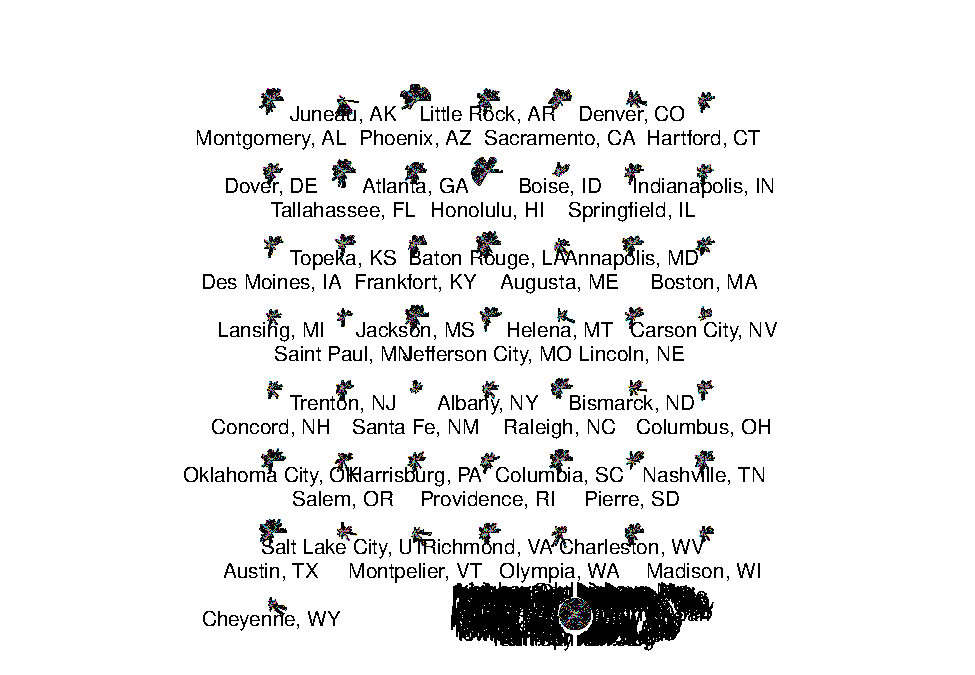
\includegraphics{graphics/chunk-distances-kmeans-setup-temp-1.pdf}

\begin{Shaded}
\begin{Highlighting}[]
\CommentTok{\#\# too busy, let\textquotesingle{}s group them}
\NormalTok{x.start =}\StringTok{ }\DecValTok{1}\NormalTok{;}
\NormalTok{x.end =}\StringTok{ }\DecValTok{10}\NormalTok{;}
\ControlFlowTok{for}\NormalTok{(i }\ControlFlowTok{in} \DecValTok{1}\OperatorTok{:}\DecValTok{5}\NormalTok{)}
\NormalTok{  \{}
  \KeywordTok{stars}\NormalTok{( whichX[x.start}\OperatorTok{:}\NormalTok{x.end,] , }
          \DataTypeTok{len =} \FloatTok{0.5}\NormalTok{, }\DataTypeTok{key.loc=}\KeywordTok{c}\NormalTok{(}\DecValTok{6}\NormalTok{,}\DecValTok{2}\NormalTok{), }\DataTypeTok{draw.segments =} \OtherTok{TRUE}\NormalTok{);}
\NormalTok{  x.start =}\StringTok{ }\DecValTok{1} \OperatorTok{+}\StringTok{ }\NormalTok{x.end;}
\NormalTok{  x.end =}\StringTok{ }\DecValTok{10} \OperatorTok{+}\StringTok{ }\NormalTok{x.end;}
\NormalTok{  \}}
\end{Highlighting}
\end{Shaded}

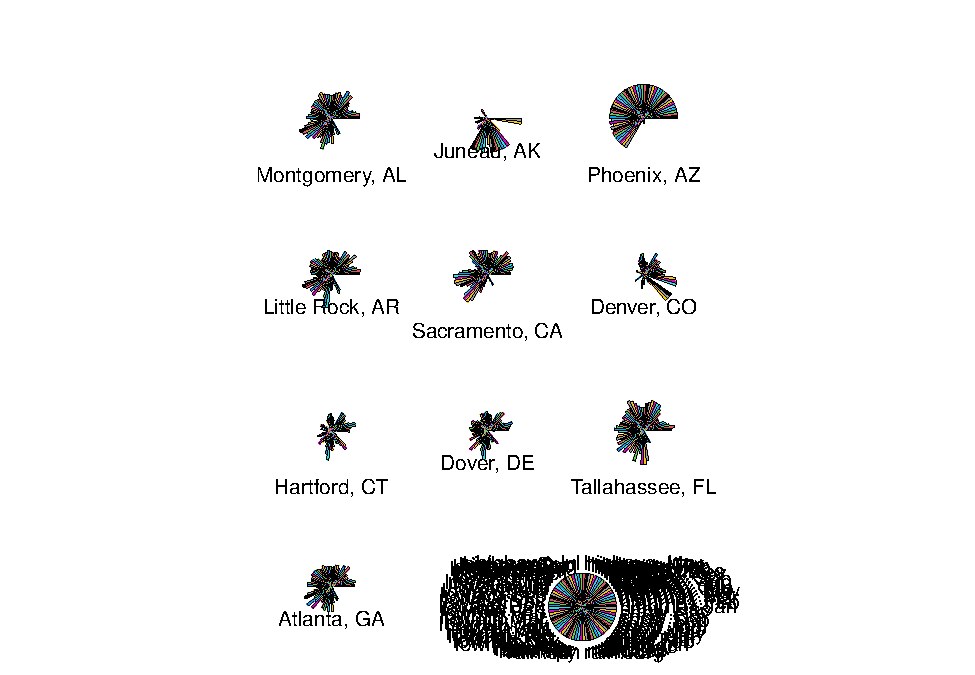
\includegraphics{graphics/chunk-distances-kmeans-setup-temp-2.pdf}
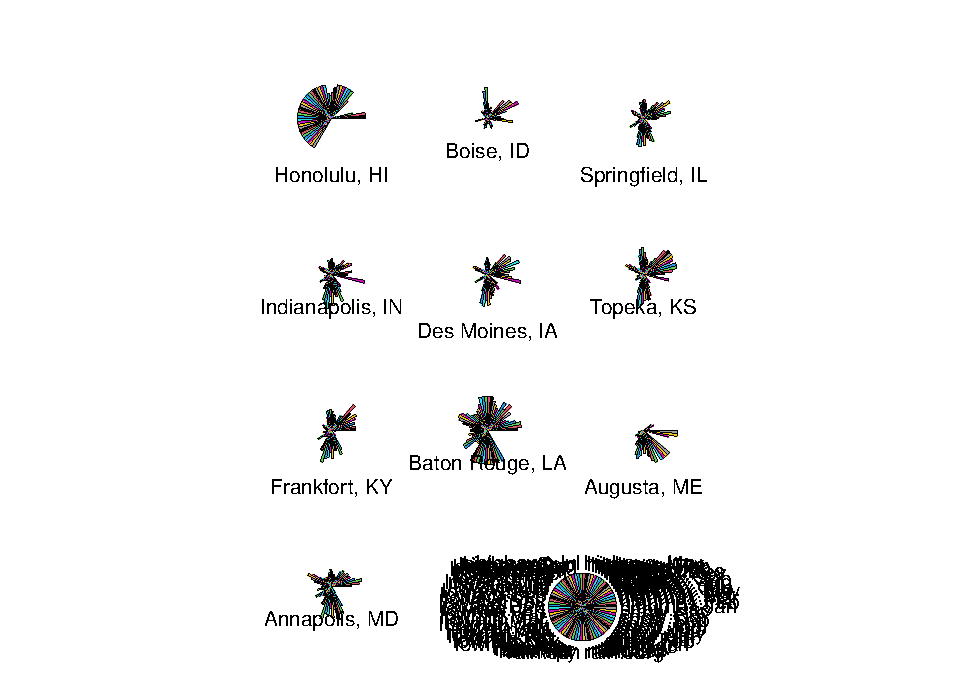
\includegraphics{graphics/chunk-distances-kmeans-setup-temp-3.pdf}
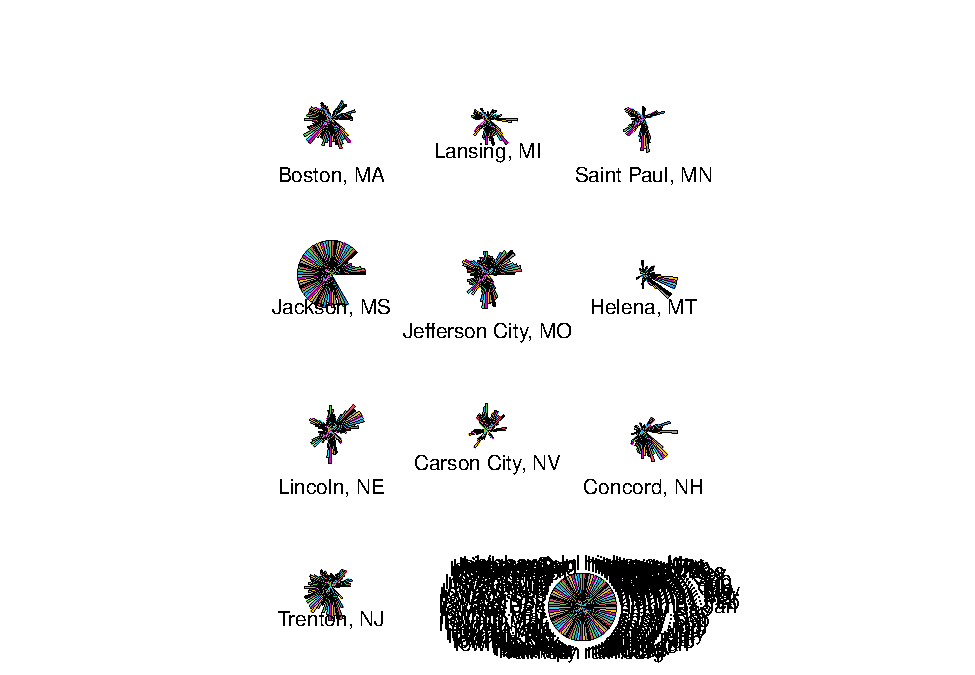
\includegraphics{graphics/chunk-distances-kmeans-setup-temp-4.pdf}
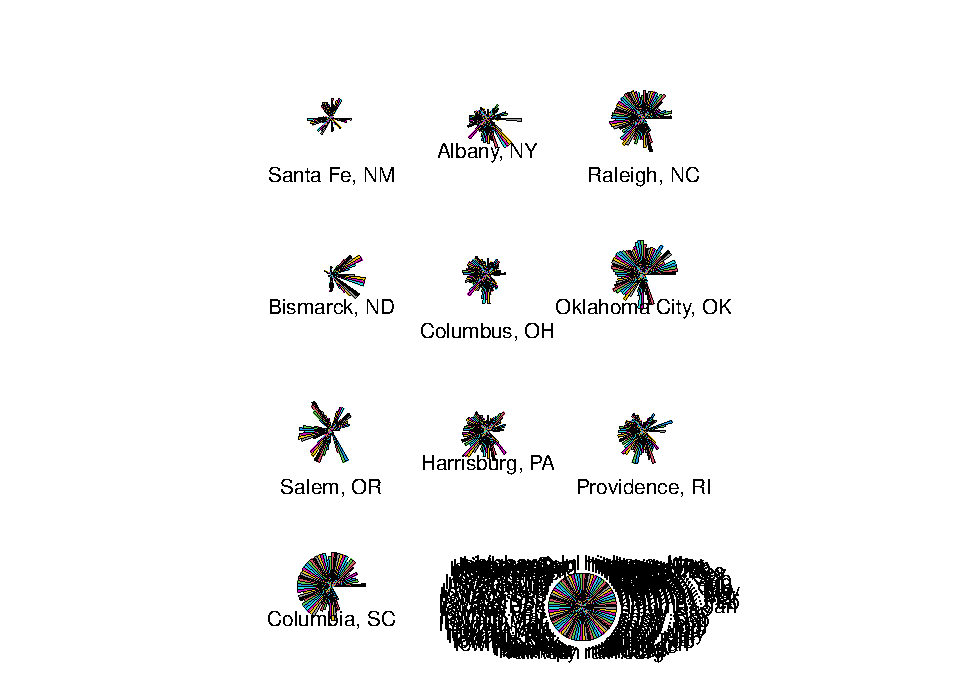
\includegraphics{graphics/chunk-distances-kmeans-setup-temp-5.pdf}
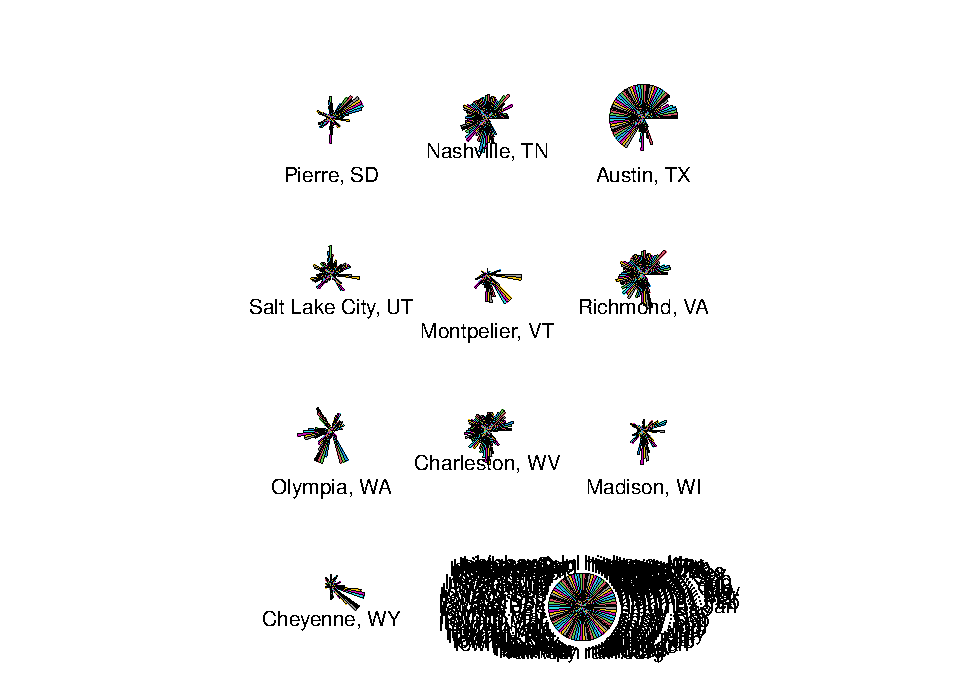
\includegraphics{graphics/chunk-distances-kmeans-setup-temp-6.pdf}

Above, you are just analyzing the general shapes. Which ones are
``fuller'' circles? Why?

Which ones are not very ``full circles''? Why?

\hypertarget{computation-of-clusterscentroids}{%
\paragraph{Computation of
Clusters/Centroids}\label{computation-of-clusterscentroids}}

\begin{Shaded}
\begin{Highlighting}[]
\NormalTok{k =}\StringTok{ }\DecValTok{12}\NormalTok{;}
\NormalTok{iterations =}\StringTok{ }\DecValTok{100}\NormalTok{;}
\NormalTok{number.starts =}\StringTok{ }\DecValTok{100}\NormalTok{;}

\NormalTok{whichX.kmeans =}\StringTok{ }\KeywordTok{kmeans}\NormalTok{(whichX, }\DecValTok{12}\NormalTok{, }
                    \DataTypeTok{iter.max=}\NormalTok{iterations, }
                    \DataTypeTok{nstart =}\NormalTok{ number.starts);  }\CommentTok{\# default algorithm}
\KeywordTok{stars}\NormalTok{(whichX.kmeans}\OperatorTok{$}\NormalTok{centers, }\DataTypeTok{len =} \FloatTok{0.5}\NormalTok{, }\DataTypeTok{key.loc =} \KeywordTok{c}\NormalTok{(}\DecValTok{10}\NormalTok{, }\DecValTok{3}\NormalTok{),}
        \DataTypeTok{main =} \StringTok{"Algorithm: DEFAULT [Hartigan{-}Wong] }\CharTok{\textbackslash{}n}\StringTok{ Stars of KMEANS=12"}\NormalTok{, }\DataTypeTok{draw.segments =} \OtherTok{TRUE}\NormalTok{);}
\end{Highlighting}
\end{Shaded}

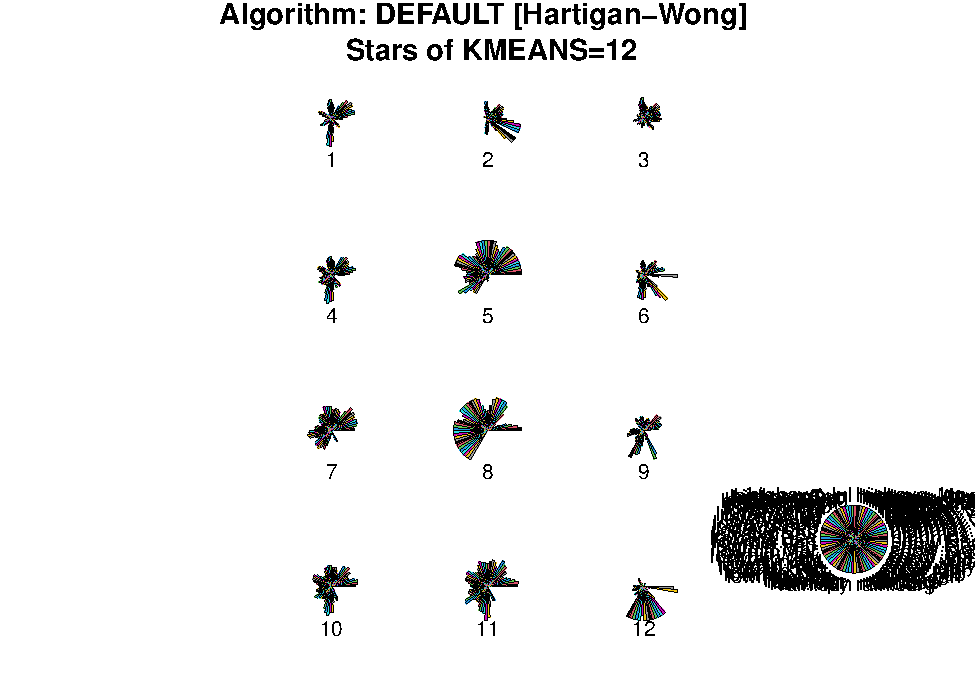
\includegraphics{graphics/chunk-distances-kmeans-run-temp-1.pdf}

\hypertarget{cluster-membership-and-centroid-attributes}{%
\paragraph{Cluster Membership and Centroid
Attributes}\label{cluster-membership-and-centroid-attributes}}

\begin{Shaded}
\begin{Highlighting}[]
\NormalTok{membership =}\StringTok{ }\KeywordTok{matrix}\NormalTok{( whichX.kmeans}\OperatorTok{$}\NormalTok{cluster, }\DataTypeTok{ncol=}\DecValTok{1}\NormalTok{);}
\NormalTok{membership =}\StringTok{ }\NormalTok{membership[}\KeywordTok{order}\NormalTok{(membership),];}
\NormalTok{membership =}\StringTok{ }\KeywordTok{as.data.frame}\NormalTok{(membership);}
        \KeywordTok{rownames}\NormalTok{(membership) =}\StringTok{ }\NormalTok{climate.df}\OperatorTok{$}\NormalTok{labels;}
        \KeywordTok{colnames}\NormalTok{(membership) =}\StringTok{ }\KeywordTok{c}\NormalTok{(}\StringTok{"Cluster"}\NormalTok{);}

\NormalTok{membership;}
\end{Highlighting}
\end{Shaded}

\begin{verbatim}
##                    Cluster
## Montgomery, AL           1
## Juneau, AK               1
## Phoenix, AZ              1
## Little Rock, AR          1
## Sacramento, CA           2
## Denver, CO               2
## Hartford, CT             2
## Dover, DE                3
## Tallahassee, FL          3
## Atlanta, GA              3
## Honolulu, HI             3
## Boise, ID                3
## Springfield, IL          4
## Indianapolis, IN         4
## Des Moines, IA           4
## Topeka, KS               4
## Frankfort, KY            4
## Baton Rouge, LA          4
## Augusta, ME              4
## Annapolis, MD            4
## Boston, MA               4
## Lansing, MI              4
## Saint Paul, MN           4
## Jackson, MS              4
## Jefferson City, MO       5
## Helena, MT               6
## Lincoln, NE              6
## Carson City, NV          6
## Concord, NH              6
## Trenton, NJ              6
## Santa Fe, NM             6
## Albany, NY               7
## Raleigh, NC              8
## Bismarck, ND             9
## Columbus, OH             9
## Oklahoma City, OK       10
## Salem, OR               10
## Harrisburg, PA          10
## Providence, RI          10
## Columbia, SC            10
## Pierre, SD              10
## Nashville, TN           10
## Austin, TX              10
## Salt Lake City, UT      11
## Montpelier, VT          11
## Richmond, VA            11
## Olympia, WA             11
## Charleston, WV          11
## Madison, WI             11
## Cheyenne, WY            12
\end{verbatim}

\begin{Shaded}
\begin{Highlighting}[]
\KeywordTok{print}\NormalTok{( }\KeywordTok{table}\NormalTok{(membership) ) ; }
\end{Highlighting}
\end{Shaded}

\begin{verbatim}
## membership
##  1  2  3  4  5  6  7  8  9 10 11 12 
##  4  3  5 12  1  6  1  1  2  8  6  1
\end{verbatim}

\begin{Shaded}
\begin{Highlighting}[]
\CommentTok{\# I believe in an older version of R these were called $centroids}
\NormalTok{attributes =}\StringTok{ }\KeywordTok{as.data.frame}\NormalTok{( whichX.kmeans}\OperatorTok{$}\NormalTok{centers );}
    \KeywordTok{rownames}\NormalTok{(attributes) =}\StringTok{ }\KeywordTok{paste0}\NormalTok{(}\StringTok{"Cluster."}\NormalTok{,}\DecValTok{1}\OperatorTok{:}\DecValTok{12}\NormalTok{);}
\NormalTok{  attributes;}
\end{Highlighting}
\end{Shaded}

\begin{verbatim}
##            highmax.Jan highmax.Feb highmax.Mar highmax.Apr highmax.May
## Cluster.1     66.25000    73.75000    88.25000    95.25000   101.75000
## Cluster.2     65.33333    71.00000    78.66667    87.66667    96.00000
## Cluster.3     67.80000    73.80000    80.80000    88.60000    96.80000
## Cluster.4     74.83333    78.66667    89.41667    94.00000    98.58333
## Cluster.5     88.00000    92.00000   100.00000   105.00000   114.00000
## Cluster.6     65.66667    67.66667    85.50000    91.66667    96.00000
## Cluster.7     79.00000    80.00000    90.00000    98.00000   107.00000
## Cluster.8     88.00000    88.00000    89.00000    91.00000    93.00000
## Cluster.9     66.00000    72.50000    79.50000    90.50000    98.00000
## Cluster.10    79.75000    84.12500    91.75000    95.25000    98.75000
## Cluster.11    85.00000    89.16667    93.33333    95.66667   101.16667
## Cluster.12    60.00000    57.00000    61.00000    72.00000    80.00000
##            highmax.Jun highmax.Jul highmax.Aug highmax.Sep highmax.Oct
## Cluster.1     106.5000    111.7500    109.2500   102.50000    94.75000
## Cluster.2     104.3333    106.3333    104.0000    99.66667    89.00000
## Cluster.3     104.0000    106.2000    104.4000   100.00000    90.60000
## Cluster.4     102.7500    107.5833    105.6667   102.91667    93.83333
## Cluster.5     122.0000    121.0000    117.0000   116.00000   107.00000
## Cluster.6      99.0000    102.0000    100.6667    97.33333    88.66667
## Cluster.7     112.0000    114.0000    112.0000   109.00000   102.00000
## Cluster.8      92.0000     94.0000     95.0000    95.00000    94.00000
## Cluster.9     101.5000    106.0000    106.0000   101.00000    91.50000
## Cluster.10    105.2500    106.6250    107.1250   103.25000    97.25000
## Cluster.11    106.1667    106.1667    107.5000   106.16667    99.00000
## Cluster.12     87.0000     89.0000     87.0000    85.00000    68.00000
##            highmax.Nov highmax.Dec highavg.Jan highavg.Feb highavg.Mar
## Cluster.1     82.25000    71.75000    30.60000    35.52500    47.42500
## Cluster.2     76.33333    66.33333    32.06667    35.80000    45.36667
## Cluster.3     77.60000    71.60000    41.58000    46.44000    55.06000
## Cluster.4     83.41667    76.50000    37.86667    42.00000    51.77500
## Cluster.5     96.00000    87.00000    67.20000    70.70000    76.90000
## Cluster.6     78.00000    69.00000    28.65000    32.66667    42.46667
## Cluster.7     86.00000    72.00000    54.40000    61.20000    66.80000
## Cluster.8     93.00000    89.00000    80.10000    80.20000    81.20000
## Cluster.9     74.00000    68.00000    46.80000    50.45000    55.20000
## Cluster.10    86.12500    80.00000    47.97500    52.13750    60.56250
## Cluster.11    89.83333    85.66667    59.46667    63.50000    70.85000
## Cluster.12    64.00000    59.00000    34.60000    36.70000    40.80000
##            highavg.Apr highavg.May highavg.Jun highavg.Jul highavg.Aug
## Cluster.1     61.07500    71.95000    81.45000    87.12500    84.97500
## Cluster.2     56.56667    66.73333    76.06667    84.60000    83.06667
## Cluster.3     62.56000    72.12000    82.26000    89.74000    87.76000
## Cluster.4     63.13333    72.58333    81.28333    85.49167    84.21667
## Cluster.5     85.20000    94.80000   103.90000   106.10000   104.40000
## Cluster.6     56.20000    67.73333    76.61667    81.05000    79.25000
## Cluster.7     72.70000    80.90000    87.90000    93.30000    92.20000
## Cluster.8     82.70000    84.60000    87.00000    87.90000    88.70000
## Cluster.9     60.00000    66.55000    72.25000    79.40000    80.05000
## Cluster.10    70.08750    78.06250    85.92500    89.68750    88.53750
## Cluster.11    77.96667    85.10000    90.55000    92.71667    92.53333
## Cluster.12    49.10000    56.90000    62.40000    63.40000    62.60000
##            highavg.Sep highavg.Oct highavg.Nov highavg.Dec lowavg.Jan
## Cluster.1     76.07500    62.22500    46.07500    32.87500   11.22500
## Cluster.2     72.16667    58.33333    43.06667    32.03333   11.06667
## Cluster.3     78.92000    65.84000    51.44000    41.30000   20.58000
## Cluster.4     77.08333    65.65000    53.80833    41.65000   21.45000
## Cluster.5     99.80000    88.50000    75.50000    66.00000   45.60000
## Cluster.6     71.26667    58.71667    46.01667    33.61667   11.80000
## Cluster.7     87.90000    77.90000    63.70000    54.30000   40.70000
## Cluster.8     88.60000    86.70000    83.90000    81.20000   66.30000
## Cluster.9     74.30000    62.15000    51.40000    45.20000   34.20000
## Cluster.10    81.80000    71.41250    61.10000    50.61250   29.77500
## Cluster.11    87.80000    79.26667    70.00000    61.35000   37.73333
## Cluster.12    56.60000    48.40000    39.80000    36.70000   26.20000
##            lowavg.Feb lowavg.Mar lowavg.Apr lowavg.May lowavg.Jun lowavg.Jul
## Cluster.1    15.65000   26.27500   38.02500   49.60000   59.32500   64.70000
## Cluster.2    14.46667   22.70000   31.20000   41.23333   49.80000   55.73333
## Cluster.3    23.84000   30.08000   35.66000   43.76000   51.78000   58.12000
## Cluster.4    24.45000   32.06667   41.79167   51.41667   60.95833   65.60833
## Cluster.5    48.70000   53.50000   60.20000   69.40000   77.70000   83.50000
## Cluster.6    14.78333   23.55000   34.81667   44.83333   54.53333   59.38333
## Cluster.7    43.70000   46.50000   49.00000   53.90000   58.40000   60.90000
## Cluster.8    66.10000   67.70000   69.40000   70.90000   73.40000   74.50000
## Cluster.9    33.70000   36.15000   38.65000   42.40000   48.45000   51.95000
## Cluster.10   32.57500   39.53750   47.98750   57.33750   66.36250   70.57500
## Cluster.11   40.95000   47.05000   53.65000   62.55000   69.68333   72.46667
## Cluster.12   27.60000   30.10000   35.30000   42.30000   48.40000   51.40000
##            lowavg.Aug lowavg.Sep lowavg.Oct lowavg.Nov lowavg.Dec lowmin.Jan
## Cluster.1    62.67500   52.70000   40.25000   27.10000   14.87500 -31.250000
## Cluster.2    53.93333   44.23333   32.86667   21.66667   11.76667 -41.666667
## Cluster.3    56.96000   48.44000   37.78000   27.74000   20.60000 -24.000000
## Cluster.4    64.10000   55.84167   44.31667   35.23333   25.60000 -20.583333
## Cluster.5    82.70000   76.90000   64.80000   52.70000   44.80000  16.000000
## Cluster.6    57.78333   49.50000   38.30000   29.63333   18.26667 -32.666667
## Cluster.7    60.50000   58.40000   52.80000   45.50000   40.40000  19.000000
## Cluster.8    75.10000   74.40000   73.40000   71.40000   68.30000  52.000000
## Cluster.9    51.65000   47.20000   41.40000   37.40000   33.30000  -9.000000
## Cluster.10   69.36250   62.23750   50.55000   40.98750   32.46250 -10.000000
## Cluster.11   72.16667   66.66667   55.75000   46.20000   39.35000   1.166667
## Cluster.12   50.20000   45.80000   39.00000   31.40000   27.80000 -20.000000
##            lowmin.Feb lowmin.Mar lowmin.Apr lowmin.May lowmin.Jun lowmin.Jul
## Cluster.1  -29.750000  -21.25000    4.00000   23.00000   36.50000   44.75000
## Cluster.2  -40.333333  -29.00000  -10.00000   12.66667   28.33333   33.66667
## Cluster.3  -23.200000   -3.40000    7.20000   20.60000   29.00000   37.40000
## Cluster.4  -19.083333   -5.75000   13.16667   27.83333   37.66667   46.25000
## Cluster.5   24.000000   25.00000   35.00000   39.00000   49.00000   63.00000
## Cluster.6  -29.500000  -20.66667    3.00000   21.83333   31.33333   36.66667
## Cluster.7   21.000000   29.00000   34.00000   37.00000   43.00000   47.00000
## Cluster.8   52.000000   53.00000   56.00000   60.00000   63.00000   63.00000
## Cluster.9   -2.500000   10.50000   23.00000   25.00000   31.00000   35.00000
## Cluster.10 -10.000000    7.75000   20.62500   32.62500   40.87500   50.62500
## Cluster.11  -1.166667   15.66667   28.50000   37.33333   48.16667   56.00000
## Cluster.12 -15.000000   -5.00000   12.00000   26.00000   32.00000   39.00000
##            lowmin.Aug lowmin.Sep lowmin.Oct lowmin.Nov lowmin.Dec  rain.Jan
## Cluster.1    40.00000   24.75000   7.250000 -14.250000 -27.250000 0.7125000
## Cluster.2    28.33333    8.00000  -7.666667 -30.000000 -37.000000 0.3733333
## Cluster.3    34.20000   22.00000   6.800000 -11.800000 -22.800000 1.0180000
## Cluster.4    41.16667   30.75000  18.666667   1.250000 -17.000000 2.7658333
## Cluster.5    58.00000   47.00000  34.000000  27.000000  22.000000 0.9100000
## Cluster.6    32.33333   22.66667  13.833333  -8.333333 -23.500000 2.2050000
## Cluster.7    48.00000   44.00000  34.000000  27.000000  17.000000 3.6300000
## Cluster.8    63.00000   65.00000  61.000000  57.000000  54.000000 0.0000000
## Cluster.9    31.50000   25.50000  16.500000   4.000000  -9.500000 6.9000000
## Cluster.10   47.00000   35.37500  23.500000   8.250000  -3.125000 3.2700000
## Cluster.11   56.00000   39.66667  27.333333  15.666667   5.833333 4.2466667
## Cluster.12   32.00000   28.00000  13.000000  -7.000000 -10.000000 7.9800000
##             rain.Feb  rain.Mar rain.Apr rain.May rain.Jun rain.Jul rain.Aug
## Cluster.1  0.8275000 1.7500000 2.812500 3.970000 4.267500 3.722500 3.545000
## Cluster.2  0.4266667 0.8366667 1.340000 2.203333 2.523333 2.090000 1.810000
## Cluster.3  0.9280000 1.2380000 1.226000 1.366000 1.068000 1.124000 1.012000
## Cluster.4  2.5316667 3.6216667 3.654167 4.325833 4.211667 4.245833 3.607500
## Cluster.5  0.9200000 0.9900000 0.280000 0.110000 0.020000 1.050000 1.000000
## Cluster.6  2.0350000 2.7483333 3.241667 3.540000 3.803333 3.728333 3.576667
## Cluster.7  3.9000000 2.8600000 1.360000 0.750000 0.210000 0.020000 0.040000
## Cluster.8  0.0000000 0.0000000 0.000000 0.000000 0.000000 0.000000 0.000000
## Cluster.9  4.9150000 4.6400000 3.175000 2.275000 1.650000 0.545000 0.690000
## Cluster.10 3.2312500 4.2062500 3.662500 4.273750 4.036250 4.125000 3.762500
## Cluster.11 4.2600000 4.6383333 3.535000 3.948333 5.225000 4.920000 4.830000
## Cluster.12 6.7100000 6.2900000 4.640000 4.960000 4.420000 5.440000 8.160000
##             rain.Sep   rain.Oct  rain.Nov rain.Dec  snow.Jan   snow.Feb
## Cluster.1   2.802500  2.2925000 1.5475000 1.005000  4.825000  4.8750000
## Cluster.2   1.390000  0.9533333 0.5966667 0.460000  7.000000  7.0000000
## Cluster.3   0.936000  1.0780000 1.0900000 1.114000  6.400000  5.1000000
## Cluster.4   3.533333  3.3458333 3.4600000 3.150833  8.133333  6.6250000
## Cluster.5   0.640000  0.5800000 0.6500000 0.880000  0.000000  0.0000000
## Cluster.6   3.361667  3.4083333 3.2833333 2.620000 17.550000 13.2666667
## Cluster.7   0.350000  1.0600000 2.4600000 3.430000  0.000000  0.0000000
## Cluster.8   0.000000  0.0000000 0.0000000 0.000000  0.000000  0.0000000
## Cluster.9   1.495000  3.8150000 7.5650000 7.160000  1.250000  3.2000000
## Cluster.10  4.062500  3.5762500 3.6637500 3.566250  3.012500  2.3500000
## Cluster.11  3.793333  3.6366667 3.7783333 4.188333  0.200000  0.1166667
## Cluster.12 12.720000 13.2300000 8.4400000 9.230000 24.200000 15.9000000
##               snow.Mar  snow.Apr snow.May snow.Jun snow.Jul snow.Aug  snow.Sep
## Cluster.1   3.95000000 1.6750000     0.00        0        0      0.0 0.0000000
## Cluster.2   8.86666667 6.0333333     1.20        0        0      0.1 0.9333333
## Cluster.3   4.96000000 2.3400000     0.28        0        0      0.0 0.2600000
## Cluster.4   4.11666667 0.6416667     0.00        0        0      0.0 0.0000000
## Cluster.5   0.00000000 0.0000000     0.00        0        0      0.0 0.0000000
## Cluster.6  11.41666667 3.2000000     0.05        0        0      0.0 0.0000000
## Cluster.7   0.00000000 0.0000000     0.00        0        0      0.0 0.0000000
## Cluster.8   0.00000000 0.0000000     0.00        0        0      0.0 0.0000000
## Cluster.9   0.35000000 0.0000000     0.00        0        0      0.0 0.0000000
## Cluster.10  0.58750000 0.0250000     0.00        0        0      0.0 0.0000000
## Cluster.11  0.01666667 0.0000000     0.00        0        0      0.0 0.0000000
## Cluster.12  5.40000000 0.9000000     0.00        0        0      0.0 0.0000000
##              snow.Oct  snow.Nov    snow.Dec
## Cluster.1  0.50000000 2.3500000  4.92500000
## Cluster.2  3.20000000 7.2000000  8.33333333
## Cluster.3  1.30000000 4.4200000  8.12000000
## Cluster.4  0.08333333 0.9333333  5.70833333
## Cluster.5  0.00000000 0.0000000  0.00000000
## Cluster.6  0.25000000 4.1666667 15.18333333
## Cluster.7  0.00000000 0.0000000  0.00000000
## Cluster.8  0.00000000 0.0000000  0.00000000
## Cluster.9  0.00000000 0.5000000  1.85000000
## Cluster.10 0.00000000 0.1375000  1.20000000
## Cluster.11 0.00000000 0.0000000  0.01666667
## Cluster.12 0.60000000 9.2000000 13.60000000
\end{verbatim}

\hypertarget{points-summarize-findings}{%
\paragraph{(10 points) Summarize
Findings}\label{points-summarize-findings}}

\begin{itemize}
\tightlist
\item
  Identify which states share a common cluster.
\item
  For a given cluster, what are its primary characteristics
\end{itemize}

{[} Summarize your k-means findings for 12 clusters.{]}

\hypertarget{points-correlation}{%
\subsection{(15 points) Correlation}\label{points-correlation}}

Correlation, like distance, is an important feature of multivariate
analysis. So let's review some basic correlation related to our climate
data. For simplicity, let's consider ``Record High Temperature'' and
``Record Low Temperature'' and see how they correlate with other factors
we have gathered from Wikipedia.

Recall, in this table, ``Jan-Dec'' are different months of the same
temperature variable.

\begin{Shaded}
\begin{Highlighting}[]
\KeywordTok{library}\NormalTok{(Hmisc); }\CommentTok{\# p{-}values for correlation}
\end{Highlighting}
\end{Shaded}

\begin{verbatim}
## Loading required package: lattice
\end{verbatim}

\begin{verbatim}
## Loading required package: survival
\end{verbatim}

\begin{verbatim}
## Loading required package: Formula
\end{verbatim}

\begin{verbatim}
## 
## Attaching package: 'Hmisc'
\end{verbatim}

\begin{verbatim}
## The following object is masked from 'package:psych':
## 
##     describe
\end{verbatim}

\begin{verbatim}
## The following objects are masked from 'package:base':
## 
##     format.pval, units
\end{verbatim}

\begin{Shaded}
\begin{Highlighting}[]
\NormalTok{high =}\StringTok{ }\KeywordTok{subsetDataFrame}\NormalTok{(climate, }\KeywordTok{c}\NormalTok{(}\StringTok{"key"}\NormalTok{, }\StringTok{"units"}\NormalTok{), }\StringTok{"=="}\NormalTok{, }\KeywordTok{c}\NormalTok{(}\StringTok{"Record high F (C)"}\NormalTok{,}\DecValTok{1}\NormalTok{));}
\NormalTok{high =}\StringTok{ }\KeywordTok{merge}\NormalTok{(high, capitals, }\DataTypeTok{by=}\KeywordTok{c}\NormalTok{(}\StringTok{"capital"}\NormalTok{,}\StringTok{"state"}\NormalTok{));}

\NormalTok{high.X =}\StringTok{ }\NormalTok{high[,}\KeywordTok{c}\NormalTok{(}\DecValTok{5}\OperatorTok{:}\DecValTok{18}\NormalTok{,}\DecValTok{21}\NormalTok{)]; }\CommentTok{\# numeric data}
\NormalTok{high.cor =}\StringTok{ }\KeywordTok{round}\NormalTok{( }\KeywordTok{cor}\NormalTok{(high.X), }\DataTypeTok{digits=}\DecValTok{2}\NormalTok{);}
\CommentTok{\# high.cor.p = rcorr(as.matrix(high.X), type="pearson");  \# p{-}values for statistical significance ... \# str(high.cor.p);}

\CommentTok{\# examine July (idx = 7)}

\KeywordTok{as.data.frame}\NormalTok{( high.cor ) ; }\CommentTok{\# so it will render nicely in RStudio}
\end{Highlighting}
\end{Shaded}

\begin{verbatim}
##                       Jan   Feb   Mar   Apr   May   Jun   Jul   Aug   Sep   Oct
## Jan                  1.00  0.92  0.76  0.57  0.43  0.39  0.25  0.41  0.62  0.71
## Feb                  0.92  1.00  0.80  0.63  0.62  0.53  0.45  0.59  0.74  0.79
## Mar                  0.76  0.80  1.00  0.87  0.73  0.56  0.53  0.67  0.76  0.82
## Apr                  0.57  0.63  0.87  1.00  0.82  0.68  0.65  0.75  0.79  0.81
## May                  0.43  0.62  0.73  0.82  1.00  0.83  0.85  0.85  0.86  0.81
## Jun                  0.39  0.53  0.56  0.68  0.83  1.00  0.90  0.86  0.87  0.78
## Jul                  0.25  0.45  0.53  0.65  0.85  0.90  1.00  0.91  0.86  0.73
## Aug                  0.41  0.59  0.67  0.75  0.85  0.86  0.91  1.00  0.90  0.78
## Sep                  0.62  0.74  0.76  0.79  0.86  0.87  0.86  0.90  1.00  0.88
## Oct                  0.71  0.79  0.82  0.81  0.81  0.78  0.73  0.78  0.88  1.00
## Nov                  0.89  0.89  0.89  0.76  0.65  0.56  0.46  0.57  0.74  0.86
## Dec                  0.94  0.89  0.81  0.65  0.46  0.41  0.27  0.46  0.65  0.72
## latitude            -0.83 -0.80 -0.68 -0.49 -0.40 -0.30 -0.15 -0.29 -0.46 -0.67
## longitude            0.07  0.01  0.39  0.34  0.08  0.01  0.02  0.04  0.07  0.14
## population.2019.est  0.40  0.42  0.36  0.35  0.38  0.48  0.31  0.31  0.44  0.39
##                       Nov   Dec latitude longitude population.2019.est
## Jan                  0.89  0.94    -0.83      0.07                0.40
## Feb                  0.89  0.89    -0.80      0.01                0.42
## Mar                  0.89  0.81    -0.68      0.39                0.36
## Apr                  0.76  0.65    -0.49      0.34                0.35
## May                  0.65  0.46    -0.40      0.08                0.38
## Jun                  0.56  0.41    -0.30      0.01                0.48
## Jul                  0.46  0.27    -0.15      0.02                0.31
## Aug                  0.57  0.46    -0.29      0.04                0.31
## Sep                  0.74  0.65    -0.46      0.07                0.44
## Oct                  0.86  0.72    -0.67      0.14                0.39
## Nov                  1.00  0.91    -0.82      0.17                0.40
## Dec                  0.91  1.00    -0.85      0.12                0.42
## latitude            -0.82 -0.85     1.00      0.01               -0.34
## longitude            0.17  0.12     0.01      1.00               -0.10
## population.2019.est  0.40  0.42    -0.34     -0.10                1.00
\end{verbatim}

\begin{Shaded}
\begin{Highlighting}[]
\NormalTok{high.cor.july =}\StringTok{ }\NormalTok{high.cor[,}\DecValTok{7}\NormalTok{];}
\NormalTok{high.cor.july;}
\end{Highlighting}
\end{Shaded}

\begin{verbatim}
##                 Jan                 Feb                 Mar                 Apr 
##                0.25                0.45                0.53                0.65 
##                 May                 Jun                 Jul                 Aug 
##                0.85                0.90                1.00                0.91 
##                 Sep                 Oct                 Nov                 Dec 
##                0.86                0.73                0.46                0.27 
##            latitude           longitude population.2019.est 
##               -0.15                0.02                0.31
\end{verbatim}

Describe the correlation of July in ``Record high F (C)'' to the other
numeric factors printed above.

\textbf{x is correlated with y (0.00). This correlation is
positive/negative which means \ldots{} This correlation is strong/weak
because \ldots{} overall, this suggests \ldots{} }

\begin{itemize}
\item
  July perfectly correlates with July (1.00). This correlation is
  positive and very strong. This is because they are the same data.
\item
  With the months, you can note each, or plot a trend showing them, and
  discussing them briefly as a trend.
\item
  latitude is a measure of north/south, so be certain to apply the
  correlation value with some meaning. be certain you know which
  direction is positive or negative to correctly interpret the sign of
  the correlation.
\item
  longitude is a measure of east/west, so be certain \ldots{}
\item
  population is the size of the city
\item
  intuitively, which months do you think correlate most with latitude
  for this data? which correlate the least? is the correlation always
  the same sign (positive/negative), or does it change? {[}You can use
  the dataframe output to do this analysis, or create your own subset{]}
\end{itemize}

\begin{Shaded}
\begin{Highlighting}[]
\KeywordTok{library}\NormalTok{(Hmisc); }\CommentTok{\# p{-}values for correlation}

\NormalTok{low =}\StringTok{ }\KeywordTok{subsetDataFrame}\NormalTok{(climate, }\KeywordTok{c}\NormalTok{(}\StringTok{"key"}\NormalTok{, }\StringTok{"units"}\NormalTok{), }\StringTok{"=="}\NormalTok{, }\KeywordTok{c}\NormalTok{(}\StringTok{"Record low F (C)"}\NormalTok{,}\DecValTok{1}\NormalTok{));}
\NormalTok{low =}\StringTok{ }\KeywordTok{merge}\NormalTok{(low, capitals, }\DataTypeTok{by=}\KeywordTok{c}\NormalTok{(}\StringTok{"capital"}\NormalTok{,}\StringTok{"state"}\NormalTok{));}

\NormalTok{low.X =}\StringTok{ }\NormalTok{low[,}\KeywordTok{c}\NormalTok{(}\DecValTok{5}\OperatorTok{:}\DecValTok{18}\NormalTok{,}\DecValTok{21}\NormalTok{)]; }\CommentTok{\# numeric data}
\NormalTok{low.cor =}\StringTok{ }\KeywordTok{round}\NormalTok{( }\KeywordTok{cor}\NormalTok{(low.X), }\DataTypeTok{digits=}\DecValTok{2}\NormalTok{);}
\CommentTok{\# low.cor.p = rcorr(as.matrix(low.X), type="pearson");  \# p{-}values for statistical significance ... \# str(low.cor.p);}

\CommentTok{\# examine Jan (idx = 1)}

\KeywordTok{as.data.frame}\NormalTok{( low.cor ) ; }\CommentTok{\# so it will render nicely in RStudio}
\end{Highlighting}
\end{Shaded}

\begin{verbatim}
##                       Jan   Feb   Mar   Apr   May   Jun   Jul   Aug   Sep   Oct
## Jan                  1.00  0.95  0.93  0.92  0.89  0.80  0.74  0.77  0.90  0.87
## Feb                  0.95  1.00  0.94  0.92  0.86  0.75  0.70  0.72  0.88  0.86
## Mar                  0.93  0.94  1.00  0.92  0.85  0.73  0.71  0.72  0.85  0.85
## Apr                  0.92  0.92  0.92  1.00  0.91  0.82  0.78  0.81  0.93  0.89
## May                  0.89  0.86  0.85  0.91  1.00  0.93  0.88  0.88  0.95  0.93
## Jun                  0.80  0.75  0.73  0.82  0.93  1.00  0.92  0.91  0.88  0.82
## Jul                  0.74  0.70  0.71  0.78  0.88  0.92  1.00  0.96  0.87  0.77
## Aug                  0.77  0.72  0.72  0.81  0.88  0.91  0.96  1.00  0.87  0.77
## Sep                  0.90  0.88  0.85  0.93  0.95  0.88  0.87  0.87  1.00  0.94
## Oct                  0.87  0.86  0.85  0.89  0.93  0.82  0.77  0.77  0.94  1.00
## Nov                  0.91  0.92  0.90  0.89  0.89  0.81  0.75  0.75  0.92  0.93
## Dec                  0.97  0.95  0.93  0.92  0.91  0.82  0.78  0.79  0.91  0.90
## latitude            -0.72 -0.64 -0.69 -0.71 -0.72 -0.75 -0.75 -0.80 -0.72 -0.66
## longitude           -0.33 -0.36 -0.31 -0.25 -0.12 -0.05  0.09  0.02 -0.09 -0.04
## population.2019.est  0.34  0.37  0.32  0.37  0.35  0.39  0.46  0.46  0.40  0.32
##                       Nov   Dec latitude longitude population.2019.est
## Jan                  0.91  0.97    -0.72     -0.33                0.34
## Feb                  0.92  0.95    -0.64     -0.36                0.37
## Mar                  0.90  0.93    -0.69     -0.31                0.32
## Apr                  0.89  0.92    -0.71     -0.25                0.37
## May                  0.89  0.91    -0.72     -0.12                0.35
## Jun                  0.81  0.82    -0.75     -0.05                0.39
## Jul                  0.75  0.78    -0.75      0.09                0.46
## Aug                  0.75  0.79    -0.80      0.02                0.46
## Sep                  0.92  0.91    -0.72     -0.09                0.40
## Oct                  0.93  0.90    -0.66     -0.04                0.32
## Nov                  1.00  0.94    -0.70     -0.12                0.28
## Dec                  0.94  1.00    -0.71     -0.24                0.33
## latitude            -0.70 -0.71     1.00      0.01               -0.34
## longitude           -0.12 -0.24     0.01      1.00               -0.10
## population.2019.est  0.28  0.33    -0.34     -0.10                1.00
\end{verbatim}

\begin{Shaded}
\begin{Highlighting}[]
\NormalTok{low.cor.january =}\StringTok{ }\NormalTok{low.cor[,}\DecValTok{1}\NormalTok{];}
\NormalTok{low.cor.january;}
\end{Highlighting}
\end{Shaded}

\begin{verbatim}
##                 Jan                 Feb                 Mar                 Apr 
##                1.00                0.95                0.93                0.92 
##                 May                 Jun                 Jul                 Aug 
##                0.89                0.80                0.74                0.77 
##                 Sep                 Oct                 Nov                 Dec 
##                0.90                0.87                0.91                0.97 
##            latitude           longitude population.2019.est 
##               -0.72               -0.33                0.34
\end{verbatim}

Describe the correlation of January in ``Record low F (C)'' to the other
numeric factors printed above.

Similar to ``high'' writeup, but for the ``low'' data.

\hypertarget{so-what-is-data-analysis}{%
\subsection{``So What'' is DATA
ANALYSIS?}\label{so-what-is-data-analysis}}

In the social sciences (e.g., Karl Weick), the concept of ``sense
making'' refers to ``the process by which people give meaning to their
collective experiences''. I have used this framework in my
high-technology innovation research (See Figure 1 of
\url{http://www.mshaffer.com/arizona/pdf/LoneGenius.pdf}, my rubric
concept comes from learning-theory growth models: Nascent, Adolescent,
Mature.)

This final topic is reflective: we are thinking about how we think.

\hypertarget{statistics}{%
\subsubsection{Statistics}\label{statistics}}

The syllabus defined statistics as ``the discipline that concerns the
collection, organization, analysis, interpretation and presentation of
data.'' (See \url{https://en.wikipedia.org/wiki/Statistics})

There are 5 elements mentioned: collection, organization, analysis,
interpretation, and presentation of ``data''. Are those equally
weighted? That is, should we devote 20\% of our time to each of those?
Now, consider the ``analysis'' stage. I have suggested there are two
camps: exploratory and confirmatory data analysis. Are those equally
weighted? That is, should we devote 50\% of our time to each of those?
Now, in an ``equally-likely'' scenario, we would have.

\begin{Shaded}
\begin{Highlighting}[]
\NormalTok{x =}\StringTok{ }\KeywordTok{c}\NormalTok{(}\DecValTok{20}\NormalTok{,}\DecValTok{20}\NormalTok{,}\DecValTok{10}\NormalTok{,}\DecValTok{10}\NormalTok{,}\DecValTok{20}\NormalTok{,}\DecValTok{20}\NormalTok{);}
\NormalTok{x.labels =}\StringTok{ }\KeywordTok{c}\NormalTok{(}\StringTok{"collection"}\NormalTok{, }\StringTok{"organization"}\NormalTok{, }\StringTok{"EDA analysis"}\NormalTok{, }\StringTok{"CDA analysis"}\NormalTok{, }\StringTok{"interpretation"}\NormalTok{, }\StringTok{"presentation"}\NormalTok{);}
\NormalTok{x.colors =}\StringTok{ }\KeywordTok{c}\NormalTok{(}\StringTok{"blue"}\NormalTok{, }\StringTok{"lightgreen"}\NormalTok{, }\StringTok{"green"}\NormalTok{, }\StringTok{"darkgreen"}\NormalTok{, }\StringTok{"orange"}\NormalTok{, }\StringTok{"red"}\NormalTok{);}

\KeywordTok{barplot}\NormalTok{(x, }
        \DataTypeTok{col =}\NormalTok{ x.colors,}
        \DataTypeTok{ylim =} \KeywordTok{c}\NormalTok{(}\DecValTok{0}\NormalTok{, }\DecValTok{20}\NormalTok{),}
        \DataTypeTok{ylab =} \StringTok{"Proportion: (Sums to 100)"}\NormalTok{,}
        \DataTypeTok{main=}\StringTok{"Statistics as the Study of \textquotesingle{}Data\textquotesingle{}"}\NormalTok{);}


\KeywordTok{text}\NormalTok{(}\FloatTok{1.14}\OperatorTok{*}\StringTok{ }\NormalTok{(}\DecValTok{1}\OperatorTok{:}\DecValTok{6}\NormalTok{), }\KeywordTok{par}\NormalTok{(}\StringTok{"usr"}\NormalTok{)[}\DecValTok{3}\NormalTok{], }\DataTypeTok{col =}\NormalTok{ x.colors, }\DataTypeTok{labels =}\NormalTok{ x.labels, }\DataTypeTok{srt =} \DecValTok{45}\NormalTok{, }\DataTypeTok{adj =} \KeywordTok{c}\NormalTok{(}\FloatTok{1.1}\NormalTok{,}\FloatTok{1.1}\NormalTok{), }\DataTypeTok{xpd =} \OtherTok{TRUE}\NormalTok{, }\DataTypeTok{cex=}\NormalTok{.}\DecValTok{75}\NormalTok{);}
\end{Highlighting}
\end{Shaded}

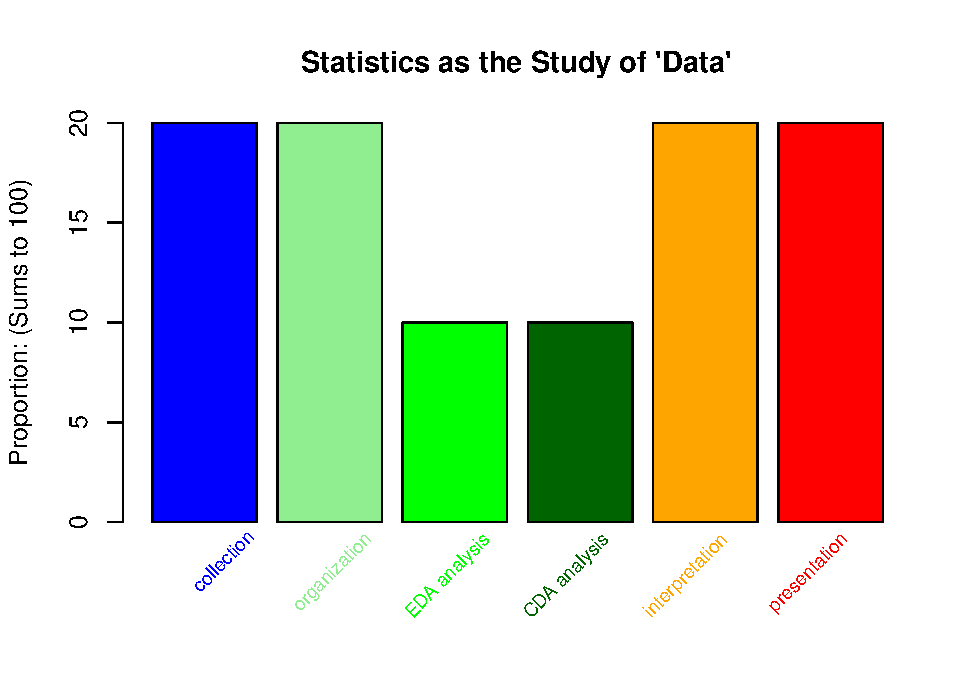
\includegraphics{graphics/chunk-conclusion-equally-likely-1.pdf}

\hypertarget{data-analytics}{%
\subsubsection{Data Analytics}\label{data-analytics}}

\textbf{Source: \url{https://data-analytics.wsu.edu/197-2/} } (Accessed
October 2010)

``Data analytics is the application of powerful new methods---drawn from
computer science, mathematics and statistics, and domain sciences---to
collect, curate, analyze, discover and communicate knowledge from `big
data'.'' \url{https://data-analytics.wsu.edu/} (Accessed October 2010)

\hypertarget{importance-of-data}{%
\paragraph{Importance of `Data'}\label{importance-of-data}}

I love data.

I also love math/physics. I also love exploratory data analysis. I also
love computational statistics or statistical computing
\url{https://en.wikipedia.org/wiki/Computational_statistics}. I also
love thinking about developing the one graphic to summarize data most
effectively.

\hypertarget{apprenticeship-as-learning-a-trade}{%
\paragraph{Apprenticeship as Learning a
Trade}\label{apprenticeship-as-learning-a-trade}}

The idea of sharing in the learning process is an important aspect of
the apprenticeship model. You are learning a trade (data analytics). I
have experience in this trade. My job as the instructor is to provide
you with a variety of ``situated-learning'' experiences To help you
understand the nature of the trade. This exam is an example of such an
experience.

\hypertarget{tools-of-the-trade}{%
\paragraph{Tools of the Trade}\label{tools-of-the-trade}}

Below are the core requirements for the data analytics program:

\begin{itemize}
\tightlist
\item
  Calculus and linear algebra (10 credits)
\item
  Computer science fundamentals (11 credits)
\item
  Machine learning and data management (9 credits)
\item
  Statistics (15 credits)
\item
  Data analytics introduction, ethics \& project-focused * capstone
  experience (9 credits)
\end{itemize}

These are not the tools of the trade, but hopefully, they introduce you
to key tools of the trade. What exactly are tools of the trade? {[}You
will have an opportunity to write a response below.{]}

\hypertarget{dimensional-reduction-an-axiomatic-view}{%
\paragraph{Dimensional Reduction, an Axiomatic
View}\label{dimensional-reduction-an-axiomatic-view}}

This video was recently shared with me that highlights some distinctions
among persons practicing various forms of data analysis
\url{https://www.youtube.com/watch?v=uHGlCi9jOWY}. As an orthogonal
projection, I would create two axes. On the horizontal axis (x-axis), I
would place ``theory of data'' to the left and ``application of data''
toward the right. On the vertical axis (y-axis), I would place ``care
for data integrity'' at the top and ``less care for data integrity'' at
the bottom.

\hypertarget{skills-of-the-trade}{%
\paragraph{Skills of the Trade}\label{skills-of-the-trade}}

As someone that is coming from industry, having hired young people like
you out of Computer Science, Electrical-Computer Engineering, I have
opinions related to skills of the trade.

\begin{itemize}
\tightlist
\item
  Can you acquire an appreciation for ``data intimacy''?
\item
  Can you track and document how data is curated?
\item
  Can you track and document the analyses you perform? Can you recreate
  them? Do you have basic version-control protocols in place?
\item
  Can you view data from multiple perspectives and synthesize those
  perspectives to identify the central them of the data? Can you be
  objective? Can you try and identify objective metrics to enlighten
  your understanding about the essence of data?
\item
  Can you experiment with different visualizations in search of an
  optimal ``one graphic'' result? Do you have practice using various
  visualization tools? Can you comprehend which visualization tool is
  appropriate for messaging (communicating results) to a particular
  audience?
\item
  Can you communicate and defend your findings to a particular audience?
  Are your communications professional? Is the final work product both
  simple and comprehensive: simple in its summary findings and
  comprehensive in its ability to be replicated and audited as
  necessary.
\end{itemize}

\hypertarget{points-your-opinion-of-data-analytics}{%
\subsection{(20 points) YOUR OPINION OF DATA
ANALYTICS}\label{points-your-opinion-of-data-analytics}}

{[}This is worth 20 points.

Specifically, address:

\begin{enumerate}
\def\labelenumi{(\arabic{enumi})}
\tightlist
\item
  what proportion of ``statistics'' should be divided among: collection,
  organization, analysis, interpretation, and presentation of ``data''
  \ldots{} providing a \texttt{barplot} of your opinion within your
  response would seem appropriate
\end{enumerate}

\begin{Shaded}
\begin{Highlighting}[]
\NormalTok{x =}\StringTok{ }\KeywordTok{c}\NormalTok{(}\DecValTok{20}\NormalTok{,}\DecValTok{20}\NormalTok{,}\DecValTok{10}\NormalTok{,}\DecValTok{10}\NormalTok{,}\DecValTok{20}\NormalTok{,}\DecValTok{20}\NormalTok{);  }\CommentTok{\#\# change these values and discuss ...}
\NormalTok{x.labels =}\StringTok{ }\KeywordTok{c}\NormalTok{(}\StringTok{"collection"}\NormalTok{, }\StringTok{"organization"}\NormalTok{, }\StringTok{"EDA analysis"}\NormalTok{, }\StringTok{"CDA analysis"}\NormalTok{, }\StringTok{"interpretation"}\NormalTok{, }\StringTok{"presentation"}\NormalTok{);}
\NormalTok{x.colors =}\StringTok{ }\KeywordTok{c}\NormalTok{(}\StringTok{"blue"}\NormalTok{, }\StringTok{"lightgreen"}\NormalTok{, }\StringTok{"green"}\NormalTok{, }\StringTok{"darkgreen"}\NormalTok{, }\StringTok{"orange"}\NormalTok{, }\StringTok{"red"}\NormalTok{);}

\KeywordTok{barplot}\NormalTok{(x, }
        \DataTypeTok{col =}\NormalTok{ x.colors,}
        \DataTypeTok{ylim =} \KeywordTok{c}\NormalTok{(}\DecValTok{0}\NormalTok{, }\KeywordTok{max}\NormalTok{(x)),}
        \DataTypeTok{ylab =} \StringTok{"Proportion: (Sums to 100)"}\NormalTok{,}
        \DataTypeTok{main=}\StringTok{"Statistics as the Study of \textquotesingle{}Data\textquotesingle{}"}\NormalTok{);}


\KeywordTok{text}\NormalTok{(}\FloatTok{1.14}\OperatorTok{*}\StringTok{ }\NormalTok{(}\DecValTok{1}\OperatorTok{:}\DecValTok{6}\NormalTok{), }\KeywordTok{par}\NormalTok{(}\StringTok{"usr"}\NormalTok{)[}\DecValTok{3}\NormalTok{], }\DataTypeTok{col =}\NormalTok{ x.colors, }\DataTypeTok{labels =}\NormalTok{ x.labels, }\DataTypeTok{srt =} \DecValTok{45}\NormalTok{, }\DataTypeTok{adj =} \KeywordTok{c}\NormalTok{(}\FloatTok{1.1}\NormalTok{,}\FloatTok{1.1}\NormalTok{), }\DataTypeTok{xpd =} \OtherTok{TRUE}\NormalTok{, }\DataTypeTok{cex=}\NormalTok{.}\DecValTok{75}\NormalTok{);}
\end{Highlighting}
\end{Shaded}

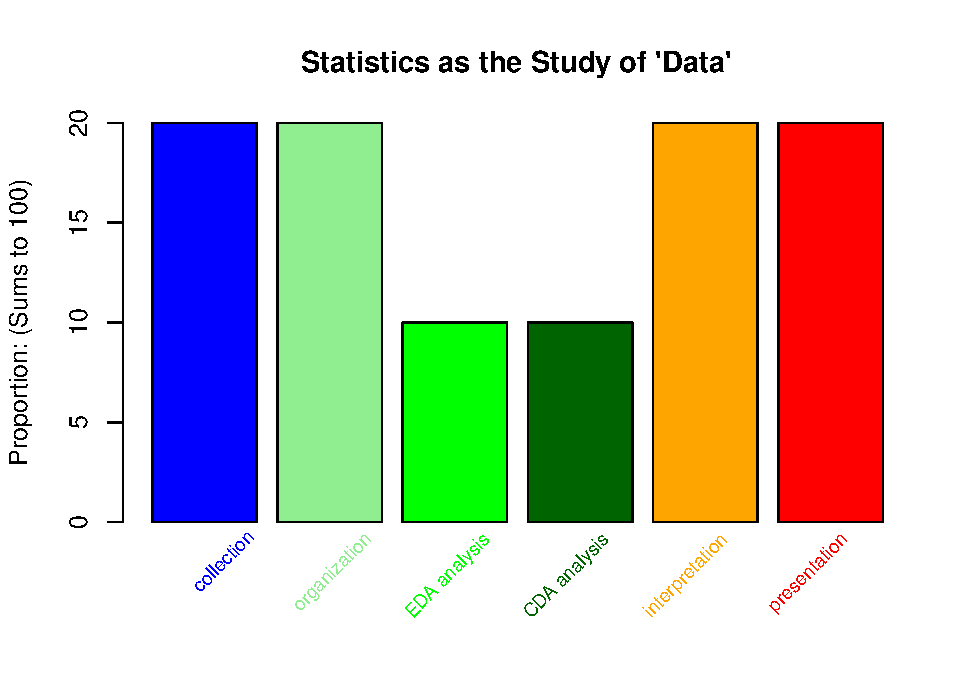
\includegraphics{graphics/chunk-conclusion-student-perspective-1.pdf}

\begin{enumerate}
\def\labelenumi{(\arabic{enumi})}
\setcounter{enumi}{1}
\item
  what tools of the trade should you be acquiring from the core courses?
  how are you doing in that acquisition process (e.g., tool X is
  \ldots{} and right now I feel like my understanding/proficiency of
  tool X \ldots{} ) \ldots{}
\item
  utilize the provided \texttt{plot} script to place the coure-course
  categories on the proposed x-y graph related to analytics practice
  (Applied vs Theoretical) and care of data integrity (Great Care vs
  Little Care) \ldots{} Also place your personal assessment on the plot
  script provided
\item
  evaluate your skill-level on the six ``skills of the trade'': Emerging
  (Nascent), Developing (Adolescent), Mastering (Mature). explain your
  evaluation and include other important skills you believe are relevant
  that are not included
\item
  Any other comments you would like to share.
\end{enumerate}

{]}

\begin{Shaded}
\begin{Highlighting}[]
\CommentTok{\# x is {-}1 for perfectly theoretical}
\CommentTok{\# x is 1 for perfectly applied}

\CommentTok{\# y is {-}1 for no care whatsoever for data integrity}
\CommentTok{\# y is 1 is perfect care for data integrity}

\CommentTok{\#\#\#\#\#\#\#\#\#\#\#\#\#\#\#\#\#\#\#\#\#\#\#\#\#\#\# basic plot setup \#\#\#\#\#}
\KeywordTok{plot}\NormalTok{(}\DecValTok{0}\NormalTok{,}\DecValTok{0}\NormalTok{, }\DataTypeTok{col=}\StringTok{"white"}\NormalTok{, }
  \DataTypeTok{ylim=}\KeywordTok{c}\NormalTok{(}\OperatorTok{{-}}\FloatTok{1.5}\NormalTok{,}\FloatTok{1.5}\NormalTok{), }\DataTypeTok{xlim=}\KeywordTok{c}\NormalTok{(}\OperatorTok{{-}}\FloatTok{1.5}\NormalTok{,}\FloatTok{1.5}\NormalTok{),}
  \DataTypeTok{xlab =} \StringTok{""}\NormalTok{,}
  \DataTypeTok{ylab =} \StringTok{""}\NormalTok{,}
  \DataTypeTok{xaxt =} \StringTok{\textquotesingle{}n\textquotesingle{}}\NormalTok{, }\DataTypeTok{bty =} \StringTok{\textquotesingle{}n\textquotesingle{}}\NormalTok{, }\DataTypeTok{yaxt =} \StringTok{\textquotesingle{}n\textquotesingle{}}\NormalTok{,}
  \DataTypeTok{main =} \StringTok{"Axiomatic Perspective on Practice/Care"}\NormalTok{,}
\NormalTok{  );}
\KeywordTok{segments}\NormalTok{(}\OperatorTok{{-}}\DecValTok{1}\NormalTok{,}\DecValTok{0}\NormalTok{,}\DecValTok{1}\NormalTok{,}\DecValTok{0}\NormalTok{, }\DataTypeTok{col=}\StringTok{"\#999999"}\NormalTok{);}
\KeywordTok{segments}\NormalTok{(}\DecValTok{0}\NormalTok{,}\OperatorTok{{-}}\DecValTok{1}\NormalTok{,}\DecValTok{0}\NormalTok{,}\DecValTok{1}\NormalTok{, }\DataTypeTok{col=}\StringTok{"\#999999"}\NormalTok{);}
\KeywordTok{text}\NormalTok{(}\OperatorTok{{-}}\FloatTok{1.1}\NormalTok{,}\DecValTok{0}\NormalTok{, }\StringTok{"Theoretical Data Practice"}\NormalTok{, }\DataTypeTok{cex=}\FloatTok{0.5}\NormalTok{, }\DataTypeTok{srt =} \DecValTok{90}\NormalTok{);}
\KeywordTok{text}\NormalTok{(}\FloatTok{1.1}\NormalTok{,}\DecValTok{0}\NormalTok{, }\StringTok{"Applied Data Practice"}\NormalTok{, }\DataTypeTok{cex=}\FloatTok{0.5}\NormalTok{, }\DataTypeTok{srt =} \DecValTok{{-}90}\NormalTok{);}
\KeywordTok{text}\NormalTok{(}\DecValTok{0}\NormalTok{,}\FloatTok{1.1}\NormalTok{, }\StringTok{"Great Care for Data Integrity"}\NormalTok{, }\DataTypeTok{cex=}\FloatTok{0.5}\NormalTok{, }\DataTypeTok{srt =} \DecValTok{0}\NormalTok{);}
\KeywordTok{text}\NormalTok{(}\DecValTok{0}\NormalTok{,}\OperatorTok{{-}}\FloatTok{1.1}\NormalTok{, }\StringTok{"Little Care for Data Integrity"}\NormalTok{, }\DataTypeTok{cex=}\FloatTok{0.5}\NormalTok{, }\DataTypeTok{srt =} \DecValTok{0}\NormalTok{);}
\CommentTok{\#\#\#\#\#\#\#\#\#\#\#\#\#\#\#\#\#\#\#\#\#\#\#\#\#\#\# basic plot setup \#\#\#\#\#}


\CommentTok{\#\#\#\#\#\#\#\#\#\#\#\#\#\#\#\#\#\#\#\#\#\#\#\#\#\#\# you can add elements here \#\#\#\#\#}
\CommentTok{\#\# this point represents the professor\textquotesingle{}s self{-}perception}
\KeywordTok{points}\NormalTok{(}\FloatTok{0.75}\NormalTok{, }\FloatTok{0.95}\NormalTok{, }\DataTypeTok{pch=}\DecValTok{20}\NormalTok{, }\DataTypeTok{col=}\StringTok{"blue"}\NormalTok{);}
\KeywordTok{text}\NormalTok{(}\FloatTok{0.75}\NormalTok{, }\FloatTok{0.95}\NormalTok{, }\StringTok{"Shaffer (self)"}\NormalTok{, }\DataTypeTok{col=}\StringTok{"blue"}\NormalTok{, }\DataTypeTok{cex=}\FloatTok{0.75}\NormalTok{, }\DataTypeTok{srt =} \DecValTok{45}\NormalTok{, }\DataTypeTok{pos=}\DecValTok{3}\NormalTok{);}
\end{Highlighting}
\end{Shaded}

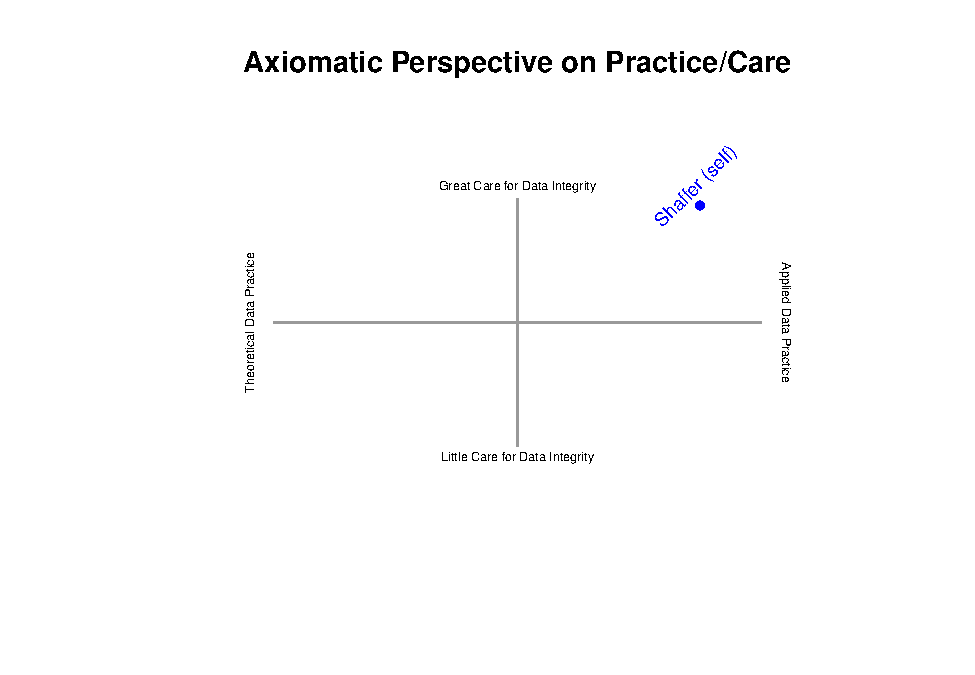
\includegraphics{graphics/chunk-conclusion-analysis-data-1.pdf}

\begin{Shaded}
\begin{Highlighting}[]
\CommentTok{\#\#\#\#\#\#\#\#\#\#\#\#\#  }\AlertTok{TODO}\CommentTok{ \#\#\#\#\#\# ... maybe change color for each data point}

\CommentTok{\# https://brand.wsu.edu/visual/colors/}
\CommentTok{\# crimson = \#981e32}
\CommentTok{\# you need to change the x,y from 0,0 ...}
\CommentTok{\# you can change col ... cex (font size), srt (angle), and pos = 1,2,3,4}
\CommentTok{\# }
\CommentTok{\# points(0, 0, pch=20, col="\#981e32");}
\CommentTok{\# text(0, 0, "Student (self)", col="\#981e32", cex=0.75, srt = 45, pos=3);}
\CommentTok{\# }
\CommentTok{\# \#\# evaluate the Course Categories of Tools of the Trade}
\CommentTok{\# \#\# give them a score}
\CommentTok{\# }
\CommentTok{\# points(0, 0, pch=20, col="\#981e32");}
\CommentTok{\# text(0, 0, "Math(s)", col="\#981e32", cex=0.5, srt = 45, pos=3);}
\CommentTok{\# }
\CommentTok{\# }
\CommentTok{\# points(0, 0, pch=20, col="\#981e32");}
\CommentTok{\# text(0, 0, "Computer Science", col="\#981e32", cex=0.5, srt = 45, pos=3);}
\CommentTok{\# }
\CommentTok{\# points(0, 0, pch=20, col="\#981e32");}
\CommentTok{\# text(0, 0, "Machine learning", col="\#981e32", cex=0.5, srt = 45, pos=3);}
\CommentTok{\# }
\CommentTok{\# points(0, 0, pch=20, col="\#981e32");}
\CommentTok{\# text(0, 0, "Statistics", col="\#981e32", cex=0.5, srt = 45, pos=3);}
\CommentTok{\# }
\CommentTok{\# points(0, 0, pch=20, col="\#981e32");}
\CommentTok{\# text(0, 0, "Data analytics", col="\#981e32", cex=0.5, srt = 45, pos=3);}
\CommentTok{\# }
\CommentTok{\# \# You have a track (e.g., Business)}
\CommentTok{\# points(0, 0, pch=20, col="\#981e32");}
\CommentTok{\# text(0, 0, "Core discipline", col="\#981e32", cex=0.5, srt = 45, pos=3);}
\end{Highlighting}
\end{Shaded}


\end{document}
